% Latex header for doxygen 1.8.13
\documentclass[twoside]{article}

% Packages required by doxygen
\usepackage{fixltx2e}
\usepackage{calc}
\usepackage{doxygen}
\usepackage[export]{adjustbox} % also loads graphicx
\usepackage{graphicx}
\usepackage[utf8]{inputenc}
\usepackage{makeidx}
\usepackage{multicol}
\usepackage{multirow}
\PassOptionsToPackage{warn}{textcomp}
\usepackage{textcomp}
\usepackage[nointegrals]{wasysym}
\usepackage[table]{xcolor}

% NLS support packages
\usepackage[french]{babel}

% Font selection
\usepackage[T1]{fontenc}
\usepackage[scaled=.90]{helvet}
\usepackage{courier}
\usepackage{amssymb}
\usepackage{sectsty}
\renewcommand{\familydefault}{\sfdefault}
\allsectionsfont{%
  \fontseries{bc}\selectfont%
  \color{darkgray}%
}
\renewcommand{\DoxyLabelFont}{%
  \fontseries{bc}\selectfont%
  \color{darkgray}%
}
\newcommand{\+}{\discretionary{\mbox{\scriptsize$\hookleftarrow$}}{}{}}

% Page & text layout
\usepackage{geometry}
\geometry{%
  a4paper,%
  top=2cm,%
  bottom=2cm,%
  left=1.2cm,%
  right=1.2cm%
}
\tolerance=750
\hfuzz=15pt
\hbadness=750
\setlength{\emergencystretch}{15pt}
\setlength{\parindent}{0cm}
\setlength{\parskip}{3ex plus 2ex minus 2ex}
\makeatletter
\renewcommand{\paragraph}{%
  \@startsection{paragraph}{4}{0ex}{-1.0ex}{1.0ex}{%
    \normalfont\normalsize\bfseries\SS@parafont%
  }%
}
\renewcommand{\subparagraph}{%
  \@startsection{subparagraph}{5}{0ex}{-1.0ex}{1.0ex}{%
    \normalfont\normalsize\bfseries\SS@subparafont%
  }%
}
\makeatother

% Headers & footers
\usepackage{fancyhdr}
\pagestyle{fancyplain}
\fancyhead[LE]{\fancyplain{}{\bfseries\thepage}}
\fancyhead[CE]{\fancyplain{}{}}
\fancyhead[RE]{\fancyplain{}{\bfseries\leftmark}}
\fancyhead[LO]{\fancyplain{}{\bfseries\rightmark}}
\fancyhead[CO]{\fancyplain{}{}}
\fancyhead[RO]{\fancyplain{}{\bfseries\thepage}}
\fancyfoot[LE]{\fancyplain{}{\bfseries\scriptsize Meeting 0.\+2}}
\fancyfoot[CE]{\fancyplain{}{}}
\fancyfoot[RE]{\fancyplain{}{\bfseries\scriptsize B\+T\+S S\+N\+I\+R La\+Salle Avignon 2020 }}
\fancyfoot[LO]{\fancyplain{}{\bfseries\scriptsize B\+T\+S S\+N\+I\+R La\+Salle Avignon 2020 }}
\fancyfoot[CO]{\fancyplain{}{}}
\fancyfoot[RO]{\fancyplain{}{\bfseries\scriptsize Meeting 0.\+2}}
\renewcommand{\footrulewidth}{0.4pt}
\renewcommand{\sectionmark}[1]{%
  \markright{\thesection\ #1}%
}

% Indices & bibliography
\usepackage{natbib}
\usepackage[titles]{tocloft}
\setcounter{tocdepth}{3}
\setcounter{secnumdepth}{5}
\makeindex

% Hyperlinks (required, but should be loaded last)
\usepackage{ifpdf}
\ifpdf
  \usepackage[pdftex,pagebackref=true]{hyperref}
\else
  \usepackage[ps2pdf,pagebackref=true]{hyperref}
\fi
\hypersetup{%
  colorlinks=true,%
  linkcolor=blue,%
  citecolor=blue,%
  unicode%
}

% Custom commands
\newcommand{\clearemptydoublepage}{%
  \newpage{\pagestyle{empty}\cleardoublepage}%
}

\usepackage{caption}
\captionsetup{labelsep=space,justification=centering,font={bf},singlelinecheck=off,skip=4pt,position=top}

%===== C O N T E N T S =====

\begin{document}

% Titlepage & ToC
\hypersetup{pageanchor=false,
             bookmarksnumbered=true,
             pdfencoding=unicode
            }
\pagenumbering{alph}
\begin{titlepage}
\vspace*{7cm}

\begin{center}%
{\LARGE Meeting}\\
\vspace*{1cm}
{\large version 0.\+2}\\
\vspace*{1cm}
{\large B\+T\+S S\+N\+I\+R La\+Salle Avignon 2020}\\
\end{center}
\end{titlepage}
\pagenumbering{roman}
\tableofcontents
\pagenumbering{arabic}
\hypersetup{pageanchor=true}

%--- Begin generated contents ---
\section{Le projet}
\label{index}\hypertarget{index}{}Placé à l\textquotesingle{}extérieur d\textquotesingle{}une pièce (salle de réunion ou de travail, ...), le système {\bfseries Meeting} permettra d\textquotesingle{}accéder en temps réel aux informations de l\textquotesingle{}espace concerné \+: il affichera la disponibilité et l\textquotesingle{}état de confort et permettra de réaliser sa réservation.\hypertarget{index_section_tdm}{}\subsection{Table des matières}\label{index_section_tdm}

\begin{DoxyItemize}
\item \hyperlink{page__r_e_a_d_m_e}{R\+E\+A\+D\+ME}
\item \hyperlink{page_changelog}{Changelog}
\item \hyperlink{page_about}{A propos}
\item \hyperlink{page_licence}{Licence G\+PL}
\end{DoxyItemize}\hypertarget{index_section_infos}{}\subsection{Informations}\label{index_section_infos}
\begin{DoxyAuthor}{Auteur}
Vincent Devine \href{mailto:vincentdevine84@gmail.com}{\tt vincentdevine84@gmail.\+com} 
\end{DoxyAuthor}
\begin{DoxyDate}{Date}
2020 
\end{DoxyDate}
\begin{DoxyVersion}{Version}
0.\+2 
\end{DoxyVersion}
\begin{DoxySeeAlso}{Voir également}
\href{https://svn.riouxsvn.com/meeting/}{\tt https\+://svn.\+riouxsvn.\+com/meeting/} 
\end{DoxySeeAlso}

\section{Changelog}
\label{page_changelog}
\Hypertarget{page_changelog}
r1 $\vert$ www-\/data $\vert$ 2020-\/02-\/01 15\+:03\+:29 +0100 (sam. 01 févr. 2020) $\vert$ 1 ligne

Creating initial repository structure 
\section{R\+E\+A\+D\+ME}
\label{page__r_e_a_d_m_e}
\Hypertarget{page__r_e_a_d_m_e}
\hypertarget{page__r_e_a_d_m_e_projet}{}\subsection{Projet}\label{page__r_e_a_d_m_e_projet}
\hypertarget{page__r_e_a_d_m_e_presentation}{}\subsubsection{Présentation}\label{page__r_e_a_d_m_e_presentation}
Placé à l\textquotesingle{}extérieur d\textquotesingle{}une pièce (salle de réunion ou de travail, ...), le système {\bfseries Meeting} permettra d\textquotesingle{}accéder en temps réel aux informations de l\textquotesingle{}espace concerné \+: il affichera la disponibilité et l\textquotesingle{}état de confort et permettra de réaliser sa réservation.

L\textquotesingle{}objectif est de proposer une solution simple, alliant flexibilité et ergonomie. Le système affiche de la disponibilité d\textquotesingle{}accès et le niveau de confort d\textquotesingle{}une salle de travail ou de réunion.

Le portier connecté est composé \+:


\begin{DoxyItemize}
\item d\textquotesingle{}un micro-\/contrôleur (E\+S\+P32, Z-\/duino,...)
\item d\textquotesingle{}un écran tactile
\item d\textquotesingle{}indicateurs lumineux (Leds)
\item d\textquotesingle{}une liaison Bluetooth vers une sonde permettant d\textquotesingle{}évaluer un “indice de confort”
\end{DoxyItemize}

La sonde est composée \+:


\begin{DoxyItemize}
\item d\textquotesingle{}un capteur de température
\item d\textquotesingle{}un capteur d\textquotesingle{}hygrométrie
\item d\textquotesingle{}un capteur de qualité d\textquotesingle{}air
\end{DoxyItemize}

A partir d\textquotesingle{}une application mobile sous Android et communiquant en U\+PD via le Wi\+Fi, l\textquotesingle{}utilisateur pourra \+:


\begin{DoxyItemize}
\item Lorsqu\textquotesingle{}une salle a été sélectionnée, visualiser les informations sur la salle (son nom et des informations complémentaires qu\textquotesingle{}il pourra associer à celle-\/ci comme sa localisation, sa surface ...), sa disponibilité et les mesures en provenance du module sonde ainsi que son indice de confort.
\item configurer les informations d\textquotesingle{}une salle.
\item la possibilité de prendre une salle en indiquant une durée estimée d\textquotesingle{}occupation de celle-\/ci. Dans ce cas, le portier lui enverra un code qu\textquotesingle{}il utilisera pour augmenter la durée d\textquotesingle{}occupation ou de libérer la salle.
\end{DoxyItemize}\hypertarget{page__r_e_a_d_m_e_informations}{}\subsubsection{Informations}\label{page__r_e_a_d_m_e_informations}
\begin{DoxyAuthor}{Auteur}
Vincent Devine \href{mailto:vincentdevine84@gmail.com}{\tt vincentdevine84@gmail.\+com} 
\end{DoxyAuthor}
\begin{DoxyDate}{Date}
2020 
\end{DoxyDate}
\begin{DoxyVersion}{Version}
0.\+2 
\end{DoxyVersion}
\begin{DoxySeeAlso}{Voir également}
\href{https://svn.riouxsvn.com/meeting/}{\tt https\+://svn.\+riouxsvn.\+com/meeting/} 
\end{DoxySeeAlso}

\section{A propos}
\label{page_about}
\Hypertarget{page_about}
\begin{DoxyAuthor}{Auteur}
Vincent Devine \href{mailto:vincentdevine84@gmail.com}{\tt vincentdevine84@gmail.\+com} 
\end{DoxyAuthor}
\begin{DoxyDate}{Date}
2020 
\end{DoxyDate}
\begin{DoxyVersion}{Version}
0.\+2 
\end{DoxyVersion}
\begin{DoxySeeAlso}{Voir également}
\href{https://svn.riouxsvn.com/meeting/}{\tt https\+://svn.\+riouxsvn.\+com/meeting/} 
\end{DoxySeeAlso}

\section{Licence G\+PL}
\label{page_licence}
\Hypertarget{page_licence}
This program is free software; you can redistribute it and/or modify it under the terms of the G\+NU General Public License as published by the Free Software Foundation; either version 2 of the License, or (at your option) any later version.

This program is distributed in the hope that it will be useful, but W\+I\+T\+H\+O\+UT A\+NY W\+A\+R\+R\+A\+N\+TY; without even the implied warranty of M\+E\+R\+C\+H\+A\+N\+T\+A\+B\+I\+L\+I\+TY or F\+I\+T\+N\+E\+SS F\+OR A P\+A\+R\+T\+I\+C\+U\+L\+AR P\+U\+R\+P\+O\+SE. See the G\+NU General Public License for more details.

You should have received a copy of the G\+NU General Public License along with this program; if not, write to the Free Software Foundation, Inc., 59 Temple Place, Suite 330, Boston, MA 02111-\/1307 U\+SA 
\section{Documentation des espaces de nommage}
\hypertarget{namespacecom}{}\subsection{Paquetage com}
\label{namespacecom}\index{com@{com}}
\subsubsection*{Paquetages}
\begin{DoxyCompactItemize}
\item 
package \hyperlink{namespacecom_1_1lasalle}{lasalle}
\end{DoxyCompactItemize}

\hypertarget{namespacecom_1_1lasalle}{}\subsection{Paquetage com.\+lasalle}
\label{namespacecom_1_1lasalle}\index{com.\+lasalle@{com.\+lasalle}}
\subsubsection*{Paquetages}
\begin{DoxyCompactItemize}
\item 
package \hyperlink{namespacecom_1_1lasalle_1_1meeting}{meeting}
\end{DoxyCompactItemize}

\hypertarget{namespacecom_1_1lasalle_1_1meeting}{}\subsection{Paquetage com.\+lasalle.\+meeting}
\label{namespacecom_1_1lasalle_1_1meeting}\index{com.\+lasalle.\+meeting@{com.\+lasalle.\+meeting}}
\subsubsection*{Classes}
\begin{DoxyCompactItemize}
\item 
class \hyperlink{classcom_1_1lasalle_1_1meeting_1_1_communication}{Communication}
\begin{DoxyCompactList}\small\item\em Déclaration de la classe \hyperlink{classcom_1_1lasalle_1_1meeting_1_1_communication}{Communication}. \end{DoxyCompactList}\item 
class \hyperlink{classcom_1_1lasalle_1_1meeting_1_1_configuration_salle_activity}{Configuration\+Salle\+Activity}
\begin{DoxyCompactList}\small\item\em Déclaration de la classe \hyperlink{classcom_1_1lasalle_1_1meeting_1_1_configuration_salle_activity}{Configuration\+Salle\+Activity}. \end{DoxyCompactList}\item 
class \hyperlink{classcom_1_1lasalle_1_1meeting_1_1_main_activity}{Main\+Activity}
\begin{DoxyCompactList}\small\item\em Déclaration de la classe \hyperlink{classcom_1_1lasalle_1_1meeting_1_1_main_activity}{Main\+Activity}. \end{DoxyCompactList}\item 
class \hyperlink{classcom_1_1lasalle_1_1meeting_1_1_salle}{Salle}
\begin{DoxyCompactList}\small\item\em Déclaration de la classe \hyperlink{classcom_1_1lasalle_1_1meeting_1_1_salle}{Salle}. \end{DoxyCompactList}\item 
class \hyperlink{classcom_1_1lasalle_1_1meeting_1_1_salle_activity}{Salle\+Activity}
\begin{DoxyCompactList}\small\item\em Déclaration de la classe \hyperlink{classcom_1_1lasalle_1_1meeting_1_1_salle_activity}{Salle\+Activity}. \end{DoxyCompactList}\item 
class \hyperlink{classcom_1_1lasalle_1_1meeting_1_1_salle_adapter}{Salle\+Adapter}
\begin{DoxyCompactList}\small\item\em Déclaration de la classe \hyperlink{classcom_1_1lasalle_1_1meeting_1_1_salle_adapter}{Salle\+Adapter}. \end{DoxyCompactList}\item 
class \hyperlink{classcom_1_1lasalle_1_1meeting_1_1_salle_view_holder}{Salle\+View\+Holder}
\begin{DoxyCompactList}\small\item\em Déclaration de la classe \hyperlink{classcom_1_1lasalle_1_1meeting_1_1_salle_view_holder}{Salle\+View\+Holder}. \end{DoxyCompactList}\end{DoxyCompactItemize}

\section{Documentation des classes}
\hypertarget{classcom_1_1lasalle_1_1meeting_1_1_communication}{}\subsection{Référence de la classe com.\+lasalle.\+meeting.\+Communication}
\label{classcom_1_1lasalle_1_1meeting_1_1_communication}\index{com.\+lasalle.\+meeting.\+Communication@{com.\+lasalle.\+meeting.\+Communication}}


Déclaration de la classe \hyperlink{classcom_1_1lasalle_1_1meeting_1_1_communication}{Communication}.  




Graphe de collaboration de com.\+lasalle.\+meeting.\+Communication\+:
\nopagebreak
\begin{figure}[H]
\begin{center}
\leavevmode
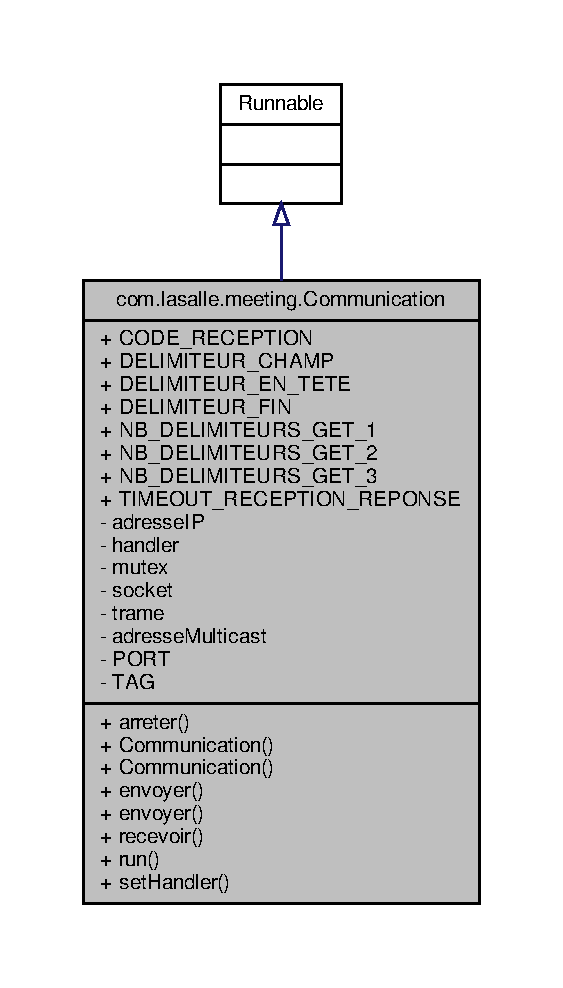
\includegraphics[width=270pt]{classcom_1_1lasalle_1_1meeting_1_1_communication__coll__graph}
\end{center}
\end{figure}
\subsubsection*{Fonctions membres publiques}
\begin{DoxyCompactItemize}
\item 
void \hyperlink{classcom_1_1lasalle_1_1meeting_1_1_communication_abf23e6b879122267b3fe10233b4010a8}{arreter} ()
\begin{DoxyCompactList}\small\item\em méthode arrétant la socket, donc la communication avec les portiers \end{DoxyCompactList}\item 
\hyperlink{classcom_1_1lasalle_1_1meeting_1_1_communication_a3d73554b2774d3274ad385b0faa27d14}{Communication} (Handler \hyperlink{classcom_1_1lasalle_1_1meeting_1_1_communication_a05fa5f360f28819a9e106e0265a74643}{handler})
\begin{DoxyCompactList}\small\item\em constructeur de communication \end{DoxyCompactList}\item 
\hyperlink{classcom_1_1lasalle_1_1meeting_1_1_communication_a38c93366f750b357d248572d85577d8f}{Communication} (int port, Handler \hyperlink{classcom_1_1lasalle_1_1meeting_1_1_communication_a05fa5f360f28819a9e106e0265a74643}{handler})
\begin{DoxyCompactList}\small\item\em constructeur de communication \end{DoxyCompactList}\item 
void \hyperlink{classcom_1_1lasalle_1_1meeting_1_1_communication_a1566200ca56ba63eec13d0ce37e6c7ee}{envoyer} (final String requete)
\begin{DoxyCompactList}\small\item\em méthode envoyant une requête à l\textquotesingle{}adresse de multicast \end{DoxyCompactList}\item 
void \hyperlink{classcom_1_1lasalle_1_1meeting_1_1_communication_a5dc5cc6c702a8d5da58c06afde637853}{envoyer} (final String requete, final String \hyperlink{classcom_1_1lasalle_1_1meeting_1_1_communication_a46e5fbc8ec97ad651d544e09121a6468}{adresse\+IP})
\begin{DoxyCompactList}\small\item\em méthode envoyant une requête à l\textquotesingle{}adresse de indiqué en paramètre \end{DoxyCompactList}\item 
void \hyperlink{classcom_1_1lasalle_1_1meeting_1_1_communication_a0344b79faa04dded3468fb8dda6baa81}{recevoir} ()
\begin{DoxyCompactList}\small\item\em méthode recevant les trames des portiers \end{DoxyCompactList}\item 
void \hyperlink{classcom_1_1lasalle_1_1meeting_1_1_communication_afe29bde1b4538990bd0a8c9b2d512efa}{run} ()
\begin{DoxyCompactList}\small\item\em méthode appelée automatiquement quand le socket reçois quelque chose \end{DoxyCompactList}\item 
void \hyperlink{classcom_1_1lasalle_1_1meeting_1_1_communication_a872d98a1793108557acccd0e695892af}{set\+Handler} (Handler \hyperlink{classcom_1_1lasalle_1_1meeting_1_1_communication_a05fa5f360f28819a9e106e0265a74643}{handler})
\begin{DoxyCompactList}\small\item\em change le handler par celui mis en paramètre \end{DoxyCompactList}\end{DoxyCompactItemize}
\subsubsection*{Attributs publics statiques}
\begin{DoxyCompactItemize}
\item 
static final int \hyperlink{classcom_1_1lasalle_1_1meeting_1_1_communication_a9cd85019614f2434af944c955519dfd1}{C\+O\+D\+E\+\_\+\+R\+E\+C\+E\+P\+T\+I\+ON} = 1
\begin{DoxyCompactList}\small\item\em code de reception correcte pour le portiers \end{DoxyCompactList}\item 
static final String \hyperlink{classcom_1_1lasalle_1_1meeting_1_1_communication_aeff38852b1f770d9a13cd5bf02090bb1}{D\+E\+L\+I\+M\+I\+T\+E\+U\+R\+\_\+\+C\+H\+A\+MP} = \char`\"{};\char`\"{}
\item 
static final String \hyperlink{classcom_1_1lasalle_1_1meeting_1_1_communication_a6560c39bb7ebc968e007e4dd98ec296c}{D\+E\+L\+I\+M\+I\+T\+E\+U\+R\+\_\+\+E\+N\+\_\+\+T\+E\+TE} = \char`\"{}\$\char`\"{}
\item 
static final String \hyperlink{classcom_1_1lasalle_1_1meeting_1_1_communication_a6f2e7cb2145496069cdf1b33d017be58}{D\+E\+L\+I\+M\+I\+T\+E\+U\+R\+\_\+\+F\+IN} = \char`\"{}\textbackslash{}r\textbackslash{}n\char`\"{}
\item 
static final int \hyperlink{classcom_1_1lasalle_1_1meeting_1_1_communication_a28886dc20c115ada2e1e3ee745805643}{N\+B\+\_\+\+D\+E\+L\+I\+M\+I\+T\+E\+U\+R\+S\+\_\+\+G\+E\+T\+\_\+1} = 6
\item 
static final int \hyperlink{classcom_1_1lasalle_1_1meeting_1_1_communication_a872d0590c8f9a71ed87484474a0c1070}{N\+B\+\_\+\+D\+E\+L\+I\+M\+I\+T\+E\+U\+R\+S\+\_\+\+G\+E\+T\+\_\+2} = 3
\item 
static final int \hyperlink{classcom_1_1lasalle_1_1meeting_1_1_communication_aa5881937f7ed66ade03b1eb16386ca9b}{N\+B\+\_\+\+D\+E\+L\+I\+M\+I\+T\+E\+U\+R\+S\+\_\+\+G\+E\+T\+\_\+3} = 1
\item 
static final int \hyperlink{classcom_1_1lasalle_1_1meeting_1_1_communication_a7cbfa2bdd8c4978f96abd43740050fe0}{T\+I\+M\+E\+O\+U\+T\+\_\+\+R\+E\+C\+E\+P\+T\+I\+O\+N\+\_\+\+R\+E\+P\+O\+N\+SE} = 30000
\begin{DoxyCompactList}\small\item\em temps maximum d\textquotesingle{}une réponse d\textquotesingle{}un portier \end{DoxyCompactList}\end{DoxyCompactItemize}
\subsubsection*{Attributs privés}
\begin{DoxyCompactItemize}
\item 
Inet\+Address \hyperlink{classcom_1_1lasalle_1_1meeting_1_1_communication_a46e5fbc8ec97ad651d544e09121a6468}{adresse\+IP} = null
\begin{DoxyCompactList}\small\item\em attribut récuperant l\textquotesingle{}adresse IP du portier \end{DoxyCompactList}\item 
Handler \hyperlink{classcom_1_1lasalle_1_1meeting_1_1_communication_a05fa5f360f28819a9e106e0265a74643}{handler}
\begin{DoxyCompactList}\small\item\em attribut permetant d\textquotesingle{}envoyer une requête par rapport a une autre activity \end{DoxyCompactList}\item 
final Reentrant\+Lock \hyperlink{classcom_1_1lasalle_1_1meeting_1_1_communication_af123afba8dcddc259017fb5c3b431dab}{mutex} = new Reentrant\+Lock()
\item 
Datagram\+Socket \hyperlink{classcom_1_1lasalle_1_1meeting_1_1_communication_a2a538f36640aecebbb833bbaf1f03858}{socket}
\begin{DoxyCompactList}\small\item\em attribut récuperant les informations de la socket \end{DoxyCompactList}\item 
String \hyperlink{classcom_1_1lasalle_1_1meeting_1_1_communication_a1c5c3782ce80717dab95ed5335929333}{trame}
\begin{DoxyCompactList}\small\item\em attribut récuperant la trame \end{DoxyCompactList}\end{DoxyCompactItemize}
\subsubsection*{Attributs privés statiques}
\begin{DoxyCompactItemize}
\item 
static final String \hyperlink{classcom_1_1lasalle_1_1meeting_1_1_communication_a6a2d2e62f87bef261a1999eb5acf8abb}{adresse\+Multicast} = \char`\"{}239.\+0.\+0.\+42\char`\"{}
\begin{DoxyCompactList}\small\item\em adresse de multicast des portiers \end{DoxyCompactList}\item 
static final int \hyperlink{classcom_1_1lasalle_1_1meeting_1_1_communication_abf48fd6a29d87d67f4941494404f1ea7}{P\+O\+RT} = 5000
\begin{DoxyCompactList}\small\item\em port d\textquotesingle{}ecoute des portiers \end{DoxyCompactList}\item 
static final String \hyperlink{classcom_1_1lasalle_1_1meeting_1_1_communication_a5d58f88df1f20b4d61edbed9a82eccab}{T\+AG} = \char`\"{}Communication\char`\"{}
\begin{DoxyCompactList}\small\item\em T\+AG utilisé dans les log. \end{DoxyCompactList}\end{DoxyCompactItemize}


\subsubsection{Description détaillée}
Déclaration de la classe \hyperlink{classcom_1_1lasalle_1_1meeting_1_1_communication}{Communication}. 

Définition à la ligne \hyperlink{_communication_8java_source_l00023}{23} du fichier \hyperlink{_communication_8java_source}{Communication.\+java}.



\subsubsection{Documentation des constructeurs et destructeur}
\mbox{\Hypertarget{classcom_1_1lasalle_1_1meeting_1_1_communication_a3d73554b2774d3274ad385b0faa27d14}\label{classcom_1_1lasalle_1_1meeting_1_1_communication_a3d73554b2774d3274ad385b0faa27d14}} 
\index{com\+::lasalle\+::meeting\+::\+Communication@{com\+::lasalle\+::meeting\+::\+Communication}!Communication@{Communication}}
\index{Communication@{Communication}!com\+::lasalle\+::meeting\+::\+Communication@{com\+::lasalle\+::meeting\+::\+Communication}}
\paragraph{\texorpdfstring{Communication()}{Communication()}\hspace{0.1cm}{\footnotesize\ttfamily [1/2]}}
{\footnotesize\ttfamily com.\+lasalle.\+meeting.\+Communication.\+Communication (\begin{DoxyParamCaption}\item[{Handler}]{handler }\end{DoxyParamCaption})}



constructeur de communication 


\begin{DoxyParams}{Paramètres}
{\em handler} & Handler \\
\hline
\end{DoxyParams}
\begin{DoxyReturn}{Renvoie}
void 
\end{DoxyReturn}


Définition à la ligne \hyperlink{_communication_8java_source_l00056}{56} du fichier \hyperlink{_communication_8java_source}{Communication.\+java}.



Références \hyperlink{_communication_8java_source_l00039}{com.\+lasalle.\+meeting.\+Communication.\+handler}, et \hyperlink{_communication_8java_source_l00031}{com.\+lasalle.\+meeting.\+Communication.\+T\+I\+M\+E\+O\+U\+T\+\_\+\+R\+E\+C\+E\+P\+T\+I\+O\+N\+\_\+\+R\+E\+P\+O\+N\+SE}.


\begin{DoxyCode}
00057     \{
00058         this.\hyperlink{classcom_1_1lasalle_1_1meeting_1_1_communication_a05fa5f360f28819a9e106e0265a74643}{handler} = \hyperlink{classcom_1_1lasalle_1_1meeting_1_1_communication_a05fa5f360f28819a9e106e0265a74643}{handler};
00059         \textcolor{keywordflow}{try}
00060         \{
00061             \hyperlink{classcom_1_1lasalle_1_1meeting_1_1_communication_a2a538f36640aecebbb833bbaf1f03858}{socket} = \textcolor{keyword}{new} DatagramSocket(\hyperlink{classcom_1_1lasalle_1_1meeting_1_1_communication_abf48fd6a29d87d67f4941494404f1ea7}{PORT});
00062             \hyperlink{classcom_1_1lasalle_1_1meeting_1_1_communication_a2a538f36640aecebbb833bbaf1f03858}{socket}.setSoTimeout(\hyperlink{classcom_1_1lasalle_1_1meeting_1_1_communication_a3d73554b2774d3274ad385b0faa27d14}{Communication}.TIMEOUT\_RECEPTION\_REPONSE);
00063         \}
00064         \textcolor{keywordflow}{catch} (SocketException se)
00065         \{
00066             se.printStackTrace();
00067         \}
00068 
00069         \textcolor{keywordflow}{try}
00070         \{
00071             this.\hyperlink{classcom_1_1lasalle_1_1meeting_1_1_communication_a46e5fbc8ec97ad651d544e09121a6468}{adresseIP} = InetAddress.getByName(\hyperlink{classcom_1_1lasalle_1_1meeting_1_1_communication_a6a2d2e62f87bef261a1999eb5acf8abb}{adresseMulticast});
00072         \}
00073         \textcolor{keywordflow}{catch} (UnknownHostException e)
00074         \{
00075             e.printStackTrace();
00076         \}
00077     \}
\end{DoxyCode}
\mbox{\Hypertarget{classcom_1_1lasalle_1_1meeting_1_1_communication_a38c93366f750b357d248572d85577d8f}\label{classcom_1_1lasalle_1_1meeting_1_1_communication_a38c93366f750b357d248572d85577d8f}} 
\index{com\+::lasalle\+::meeting\+::\+Communication@{com\+::lasalle\+::meeting\+::\+Communication}!Communication@{Communication}}
\index{Communication@{Communication}!com\+::lasalle\+::meeting\+::\+Communication@{com\+::lasalle\+::meeting\+::\+Communication}}
\paragraph{\texorpdfstring{Communication()}{Communication()}\hspace{0.1cm}{\footnotesize\ttfamily [2/2]}}
{\footnotesize\ttfamily com.\+lasalle.\+meeting.\+Communication.\+Communication (\begin{DoxyParamCaption}\item[{int}]{port,  }\item[{Handler}]{handler }\end{DoxyParamCaption})}



constructeur de communication 


\begin{DoxyParams}{Paramètres}
{\em handler} & Handler, port int \\
\hline
\end{DoxyParams}
\begin{DoxyReturn}{Renvoie}
void 
\end{DoxyReturn}


Définition à la ligne \hyperlink{_communication_8java_source_l00084}{84} du fichier \hyperlink{_communication_8java_source}{Communication.\+java}.



Références \hyperlink{_communication_8java_source_l00039}{com.\+lasalle.\+meeting.\+Communication.\+handler}, et \hyperlink{_communication_8java_source_l00031}{com.\+lasalle.\+meeting.\+Communication.\+T\+I\+M\+E\+O\+U\+T\+\_\+\+R\+E\+C\+E\+P\+T\+I\+O\+N\+\_\+\+R\+E\+P\+O\+N\+SE}.


\begin{DoxyCode}
00085     \{
00086         this.\hyperlink{classcom_1_1lasalle_1_1meeting_1_1_communication_a05fa5f360f28819a9e106e0265a74643}{handler} = \hyperlink{classcom_1_1lasalle_1_1meeting_1_1_communication_a05fa5f360f28819a9e106e0265a74643}{handler};
00087         \textcolor{keywordflow}{try}
00088         \{
00089             \hyperlink{classcom_1_1lasalle_1_1meeting_1_1_communication_a2a538f36640aecebbb833bbaf1f03858}{socket} = \textcolor{keyword}{new} DatagramSocket(port);
00090             \hyperlink{classcom_1_1lasalle_1_1meeting_1_1_communication_a2a538f36640aecebbb833bbaf1f03858}{socket}.setSoTimeout(\hyperlink{classcom_1_1lasalle_1_1meeting_1_1_communication_a3d73554b2774d3274ad385b0faa27d14}{Communication}.TIMEOUT\_RECEPTION\_REPONSE);
00091         \}
00092         \textcolor{keywordflow}{catch} (SocketException se)
00093         \{
00094             se.printStackTrace();
00095         \}
00096 
00097         \textcolor{keywordflow}{try}
00098         \{
00099             this.\hyperlink{classcom_1_1lasalle_1_1meeting_1_1_communication_a46e5fbc8ec97ad651d544e09121a6468}{adresseIP} = InetAddress.getByName(\hyperlink{classcom_1_1lasalle_1_1meeting_1_1_communication_a6a2d2e62f87bef261a1999eb5acf8abb}{adresseMulticast});
00100         \}
00101         \textcolor{keywordflow}{catch} (UnknownHostException e)
00102         \{
00103             e.printStackTrace();
00104         \}
00105     \}
\end{DoxyCode}


\subsubsection{Documentation des fonctions membres}
\mbox{\Hypertarget{classcom_1_1lasalle_1_1meeting_1_1_communication_abf23e6b879122267b3fe10233b4010a8}\label{classcom_1_1lasalle_1_1meeting_1_1_communication_abf23e6b879122267b3fe10233b4010a8}} 
\index{com\+::lasalle\+::meeting\+::\+Communication@{com\+::lasalle\+::meeting\+::\+Communication}!arreter@{arreter}}
\index{arreter@{arreter}!com\+::lasalle\+::meeting\+::\+Communication@{com\+::lasalle\+::meeting\+::\+Communication}}
\paragraph{\texorpdfstring{arreter()}{arreter()}}
{\footnotesize\ttfamily void com.\+lasalle.\+meeting.\+Communication.\+arreter (\begin{DoxyParamCaption}{ }\end{DoxyParamCaption})}



méthode arrétant la socket, donc la communication avec les portiers 

\begin{DoxyReturn}{Renvoie}
void 
\end{DoxyReturn}


Définition à la ligne \hyperlink{_communication_8java_source_l00235}{235} du fichier \hyperlink{_communication_8java_source}{Communication.\+java}.


\begin{DoxyCode}
00236     \{
00237         \textcolor{keywordflow}{if}(\hyperlink{classcom_1_1lasalle_1_1meeting_1_1_communication_a2a538f36640aecebbb833bbaf1f03858}{socket} == null)
00238             \textcolor{keywordflow}{return};
00239         \hyperlink{classcom_1_1lasalle_1_1meeting_1_1_communication_a2a538f36640aecebbb833bbaf1f03858}{socket}.close();
00240     \}
\end{DoxyCode}
\mbox{\Hypertarget{classcom_1_1lasalle_1_1meeting_1_1_communication_a1566200ca56ba63eec13d0ce37e6c7ee}\label{classcom_1_1lasalle_1_1meeting_1_1_communication_a1566200ca56ba63eec13d0ce37e6c7ee}} 
\index{com\+::lasalle\+::meeting\+::\+Communication@{com\+::lasalle\+::meeting\+::\+Communication}!envoyer@{envoyer}}
\index{envoyer@{envoyer}!com\+::lasalle\+::meeting\+::\+Communication@{com\+::lasalle\+::meeting\+::\+Communication}}
\paragraph{\texorpdfstring{envoyer()}{envoyer()}\hspace{0.1cm}{\footnotesize\ttfamily [1/2]}}
{\footnotesize\ttfamily void com.\+lasalle.\+meeting.\+Communication.\+envoyer (\begin{DoxyParamCaption}\item[{final String}]{requete }\end{DoxyParamCaption})}



méthode envoyant une requête à l\textquotesingle{}adresse de multicast 


\begin{DoxyParams}{Paramètres}
{\em requete} & String \\
\hline
\end{DoxyParams}
\begin{DoxyReturn}{Renvoie}
void 
\end{DoxyReturn}


Définition à la ligne \hyperlink{_communication_8java_source_l00161}{161} du fichier \hyperlink{_communication_8java_source}{Communication.\+java}.



Références \hyperlink{_communication_8java_source_l00247}{com.\+lasalle.\+meeting.\+Communication.\+run()}.



Référencé par \hyperlink{_main_activity_8java_source_l00330}{com.\+lasalle.\+meeting.\+Main\+Activity.\+rafraichir()}, \hyperlink{_salle_activity_8java_source_l00132}{com.\+lasalle.\+meeting.\+Salle\+Activity.\+set\+Listener()}, et \hyperlink{_configuration_salle_activity_8java_source_l00138}{com.\+lasalle.\+meeting.\+Configuration\+Salle\+Activity.\+set\+Listener()}.


\begin{DoxyCode}
00162     \{
00163         \textcolor{keywordflow}{if}(\hyperlink{classcom_1_1lasalle_1_1meeting_1_1_communication_a2a538f36640aecebbb833bbaf1f03858}{socket} == null)
00164             \textcolor{keywordflow}{return};
00165 
00166         \textcolor{keyword}{new} Thread()
00167         \{
00168             @Override \textcolor{keyword}{public} \textcolor{keywordtype}{void} \hyperlink{classcom_1_1lasalle_1_1meeting_1_1_communication_afe29bde1b4538990bd0a8c9b2d512efa}{run}()
00169             \{
00170                 byte[] emission = \textcolor{keyword}{new} byte[1024];
00171 
00172                 \textcolor{keywordflow}{try}
00173                 \{
00174                     emission = requete.getBytes();
00175                     DatagramPacket paquetRetour = \textcolor{keyword}{new} DatagramPacket(emission, emission.length, 
      \hyperlink{classcom_1_1lasalle_1_1meeting_1_1_communication_a46e5fbc8ec97ad651d544e09121a6468}{adresseIP}, \hyperlink{classcom_1_1lasalle_1_1meeting_1_1_communication_abf48fd6a29d87d67f4941494404f1ea7}{PORT});
00176                     \hyperlink{classcom_1_1lasalle_1_1meeting_1_1_communication_a2a538f36640aecebbb833bbaf1f03858}{socket}.send(paquetRetour);
00177                     Log.d(\hyperlink{classcom_1_1lasalle_1_1meeting_1_1_communication_a5d58f88df1f20b4d61edbed9a82eccab}{TAG}, \textcolor{stringliteral}{"send() = "} + requete);
00178                 \}
00179                 \textcolor{keywordflow}{catch} (IOException e)
00180                 \{
00181                     Log.d(\hyperlink{classcom_1_1lasalle_1_1meeting_1_1_communication_a5d58f88df1f20b4d61edbed9a82eccab}{TAG}, \textcolor{stringliteral}{"Erreur send() [socket.isClosed = "} + \hyperlink{classcom_1_1lasalle_1_1meeting_1_1_communication_a2a538f36640aecebbb833bbaf1f03858}{socket}.isClosed() + \textcolor{stringliteral}{"]"});
00182                     e.printStackTrace();
00183                 \}
00184             \}
00185         \}.start();
00186     \}
\end{DoxyCode}
\mbox{\Hypertarget{classcom_1_1lasalle_1_1meeting_1_1_communication_a5dc5cc6c702a8d5da58c06afde637853}\label{classcom_1_1lasalle_1_1meeting_1_1_communication_a5dc5cc6c702a8d5da58c06afde637853}} 
\index{com\+::lasalle\+::meeting\+::\+Communication@{com\+::lasalle\+::meeting\+::\+Communication}!envoyer@{envoyer}}
\index{envoyer@{envoyer}!com\+::lasalle\+::meeting\+::\+Communication@{com\+::lasalle\+::meeting\+::\+Communication}}
\paragraph{\texorpdfstring{envoyer()}{envoyer()}\hspace{0.1cm}{\footnotesize\ttfamily [2/2]}}
{\footnotesize\ttfamily void com.\+lasalle.\+meeting.\+Communication.\+envoyer (\begin{DoxyParamCaption}\item[{final String}]{requete,  }\item[{final String}]{adresse\+IP }\end{DoxyParamCaption})}



méthode envoyant une requête à l\textquotesingle{}adresse de indiqué en paramètre 


\begin{DoxyParams}{Paramètres}
{\em requete} & String, adresse\+IP String \\
\hline
\end{DoxyParams}
\begin{DoxyReturn}{Renvoie}
void 
\end{DoxyReturn}


Définition à la ligne \hyperlink{_communication_8java_source_l00193}{193} du fichier \hyperlink{_communication_8java_source}{Communication.\+java}.



Références \hyperlink{_communication_8java_source_l00247}{com.\+lasalle.\+meeting.\+Communication.\+run()}.


\begin{DoxyCode}
00194     \{
00195         \textcolor{keywordflow}{if}(\hyperlink{classcom_1_1lasalle_1_1meeting_1_1_communication_a2a538f36640aecebbb833bbaf1f03858}{socket} == null)
00196             \textcolor{keywordflow}{return};
00197 
00198         \textcolor{keyword}{final} InetAddress adresseIPDistante;
00199         \textcolor{keywordflow}{try}
00200         \{
00201             adresseIPDistante = InetAddress.getByName(\hyperlink{classcom_1_1lasalle_1_1meeting_1_1_communication_a46e5fbc8ec97ad651d544e09121a6468}{adresseIP});
00202         \}
00203         \textcolor{keywordflow}{catch} (UnknownHostException e)
00204         \{
00205             e.printStackTrace();
00206             \textcolor{keywordflow}{return};
00207         \}
00208 
00209         \textcolor{keyword}{new} Thread()
00210         \{
00211             @Override \textcolor{keyword}{public} \textcolor{keywordtype}{void} \hyperlink{classcom_1_1lasalle_1_1meeting_1_1_communication_afe29bde1b4538990bd0a8c9b2d512efa}{run}()
00212             \{
00213                 byte[] emission = \textcolor{keyword}{new} byte[1024];
00214 
00215                 \textcolor{keywordflow}{try}
00216                 \{
00217                     emission = requete.getBytes();
00218                     DatagramPacket paquetRetour = \textcolor{keyword}{new} DatagramPacket(emission, emission.length, 
      adresseIPDistante, \hyperlink{classcom_1_1lasalle_1_1meeting_1_1_communication_abf48fd6a29d87d67f4941494404f1ea7}{PORT});
00219                     \hyperlink{classcom_1_1lasalle_1_1meeting_1_1_communication_a2a538f36640aecebbb833bbaf1f03858}{socket}.send(paquetRetour);
00220                     Log.d(\hyperlink{classcom_1_1lasalle_1_1meeting_1_1_communication_a5d58f88df1f20b4d61edbed9a82eccab}{TAG}, \textcolor{stringliteral}{"send() "} + \hyperlink{classcom_1_1lasalle_1_1meeting_1_1_communication_a46e5fbc8ec97ad651d544e09121a6468}{adresseIP} + \textcolor{stringliteral}{" = "} + requete);
00221                 \}
00222                 \textcolor{keywordflow}{catch} (IOException e)
00223                 \{
00224                     Log.d(\hyperlink{classcom_1_1lasalle_1_1meeting_1_1_communication_a5d58f88df1f20b4d61edbed9a82eccab}{TAG}, \textcolor{stringliteral}{"Erreur send() [socket.isClosed = "} + \hyperlink{classcom_1_1lasalle_1_1meeting_1_1_communication_a2a538f36640aecebbb833bbaf1f03858}{socket}.isClosed() + \textcolor{stringliteral}{"]"});
00225                     e.printStackTrace();
00226                 \}
00227             \}
00228         \}.start();
00229     \}
\end{DoxyCode}
\mbox{\Hypertarget{classcom_1_1lasalle_1_1meeting_1_1_communication_a0344b79faa04dded3468fb8dda6baa81}\label{classcom_1_1lasalle_1_1meeting_1_1_communication_a0344b79faa04dded3468fb8dda6baa81}} 
\index{com\+::lasalle\+::meeting\+::\+Communication@{com\+::lasalle\+::meeting\+::\+Communication}!recevoir@{recevoir}}
\index{recevoir@{recevoir}!com\+::lasalle\+::meeting\+::\+Communication@{com\+::lasalle\+::meeting\+::\+Communication}}
\paragraph{\texorpdfstring{recevoir()}{recevoir()}}
{\footnotesize\ttfamily void com.\+lasalle.\+meeting.\+Communication.\+recevoir (\begin{DoxyParamCaption}{ }\end{DoxyParamCaption})}



méthode recevant les trames des portiers 

\begin{DoxyReturn}{Renvoie}
void 
\end{DoxyReturn}


Définition à la ligne \hyperlink{_communication_8java_source_l00123}{123} du fichier \hyperlink{_communication_8java_source}{Communication.\+java}.



Références \hyperlink{_communication_8java_source_l00032}{com.\+lasalle.\+meeting.\+Communication.\+C\+O\+D\+E\+\_\+\+R\+E\+C\+E\+P\+T\+I\+ON}, et \hyperlink{_communication_8java_source_l00040}{com.\+lasalle.\+meeting.\+Communication.\+trame}.



Référencé par \hyperlink{_communication_8java_source_l00247}{com.\+lasalle.\+meeting.\+Communication.\+run()}.


\begin{DoxyCode}
00124     \{
00125         byte[] reception = \textcolor{keyword}{new} byte[1024];
00126 
00127         \textcolor{keywordflow}{while} (\hyperlink{classcom_1_1lasalle_1_1meeting_1_1_communication_a2a538f36640aecebbb833bbaf1f03858}{socket} != null && !\hyperlink{classcom_1_1lasalle_1_1meeting_1_1_communication_a2a538f36640aecebbb833bbaf1f03858}{socket}.isClosed())
00128         \{
00129             \textcolor{keywordflow}{try}
00130             \{
00131                 \textcolor{keyword}{final} DatagramPacket paquetRecu = \textcolor{keyword}{new} DatagramPacket(reception, reception.length);
00132                 \hyperlink{classcom_1_1lasalle_1_1meeting_1_1_communication_a2a538f36640aecebbb833bbaf1f03858}{socket}.receive(paquetRecu);
00133 
00134                 \hyperlink{classcom_1_1lasalle_1_1meeting_1_1_communication_a1c5c3782ce80717dab95ed5335929333}{trame} = \textcolor{keyword}{new} String(paquetRecu.getData(), paquetRecu.getOffset(), paquetRecu.getLength(
      ));
00135                 Log.d(\hyperlink{classcom_1_1lasalle_1_1meeting_1_1_communication_a5d58f88df1f20b4d61edbed9a82eccab}{TAG}, \textcolor{stringliteral}{"Réception de "} + paquetRecu.getAddress().getHostAddress() + \textcolor{stringliteral}{":"} + paquetRecu
      .getPort() + \textcolor{stringliteral}{" -> "} + \hyperlink{classcom_1_1lasalle_1_1meeting_1_1_communication_a1c5c3782ce80717dab95ed5335929333}{trame});
00136 
00137                 Message msg = Message.obtain();
00138                 Bundle b = \textcolor{keyword}{new} Bundle();
00139                 b.putString(\textcolor{stringliteral}{"adresseIP"}, paquetRecu.getAddress().getHostAddress());
00140                 b.putInt(\textcolor{stringliteral}{"port"}, paquetRecu.getPort());
00141                 b.putInt(\textcolor{stringliteral}{"etat"}, \hyperlink{classcom_1_1lasalle_1_1meeting_1_1_communication_a3d73554b2774d3274ad385b0faa27d14}{Communication}.CODE\_RECEPTION);
00142                 b.putString(\textcolor{stringliteral}{"trame"}, \hyperlink{classcom_1_1lasalle_1_1meeting_1_1_communication_a1c5c3782ce80717dab95ed5335929333}{trame});
00143                 msg.setData(b);
00144                 \hyperlink{classcom_1_1lasalle_1_1meeting_1_1_communication_af123afba8dcddc259017fb5c3b431dab}{mutex}.lock();
00145                 \hyperlink{classcom_1_1lasalle_1_1meeting_1_1_communication_a05fa5f360f28819a9e106e0265a74643}{handler}.sendMessage(msg);
00146                 \hyperlink{classcom_1_1lasalle_1_1meeting_1_1_communication_af123afba8dcddc259017fb5c3b431dab}{mutex}.unlock();
00147             \}
00148             \textcolor{keywordflow}{catch} (Exception e)
00149             \{
00150                 Log.d(\hyperlink{classcom_1_1lasalle_1_1meeting_1_1_communication_a5d58f88df1f20b4d61edbed9a82eccab}{TAG}, \textcolor{stringliteral}{"Erreur recevoir() [socket.isClosed = "} + \hyperlink{classcom_1_1lasalle_1_1meeting_1_1_communication_a2a538f36640aecebbb833bbaf1f03858}{socket}.isClosed() + \textcolor{stringliteral}{"]"});
00151                 e.printStackTrace();
00152             \}
00153         \}
00154     \}
\end{DoxyCode}
\mbox{\Hypertarget{classcom_1_1lasalle_1_1meeting_1_1_communication_afe29bde1b4538990bd0a8c9b2d512efa}\label{classcom_1_1lasalle_1_1meeting_1_1_communication_afe29bde1b4538990bd0a8c9b2d512efa}} 
\index{com\+::lasalle\+::meeting\+::\+Communication@{com\+::lasalle\+::meeting\+::\+Communication}!run@{run}}
\index{run@{run}!com\+::lasalle\+::meeting\+::\+Communication@{com\+::lasalle\+::meeting\+::\+Communication}}
\paragraph{\texorpdfstring{run()}{run()}}
{\footnotesize\ttfamily void com.\+lasalle.\+meeting.\+Communication.\+run (\begin{DoxyParamCaption}{ }\end{DoxyParamCaption})}



méthode appelée automatiquement quand le socket reçois quelque chose 

\begin{DoxyReturn}{Renvoie}
void 
\end{DoxyReturn}


Définition à la ligne \hyperlink{_communication_8java_source_l00247}{247} du fichier \hyperlink{_communication_8java_source}{Communication.\+java}.



Références \hyperlink{_communication_8java_source_l00123}{com.\+lasalle.\+meeting.\+Communication.\+recevoir()}.



Référencé par \hyperlink{_communication_8java_source_l00161}{com.\+lasalle.\+meeting.\+Communication.\+envoyer()}.


\begin{DoxyCode}
00248     \{
00249         \hyperlink{classcom_1_1lasalle_1_1meeting_1_1_communication_a0344b79faa04dded3468fb8dda6baa81}{recevoir}();
00250     \}
\end{DoxyCode}
\mbox{\Hypertarget{classcom_1_1lasalle_1_1meeting_1_1_communication_a872d98a1793108557acccd0e695892af}\label{classcom_1_1lasalle_1_1meeting_1_1_communication_a872d98a1793108557acccd0e695892af}} 
\index{com\+::lasalle\+::meeting\+::\+Communication@{com\+::lasalle\+::meeting\+::\+Communication}!set\+Handler@{set\+Handler}}
\index{set\+Handler@{set\+Handler}!com\+::lasalle\+::meeting\+::\+Communication@{com\+::lasalle\+::meeting\+::\+Communication}}
\paragraph{\texorpdfstring{set\+Handler()}{setHandler()}}
{\footnotesize\ttfamily void com.\+lasalle.\+meeting.\+Communication.\+set\+Handler (\begin{DoxyParamCaption}\item[{Handler}]{handler }\end{DoxyParamCaption})}



change le handler par celui mis en paramètre 


\begin{DoxyParams}{Paramètres}
{\em handler} & Handler \\
\hline
\end{DoxyParams}
\begin{DoxyReturn}{Renvoie}
void 
\end{DoxyReturn}


Définition à la ligne \hyperlink{_communication_8java_source_l00112}{112} du fichier \hyperlink{_communication_8java_source}{Communication.\+java}.



Références \hyperlink{_communication_8java_source_l00039}{com.\+lasalle.\+meeting.\+Communication.\+handler}.


\begin{DoxyCode}
00113     \{
00114         \hyperlink{classcom_1_1lasalle_1_1meeting_1_1_communication_af123afba8dcddc259017fb5c3b431dab}{mutex}.lock();
00115         this.\hyperlink{classcom_1_1lasalle_1_1meeting_1_1_communication_a05fa5f360f28819a9e106e0265a74643}{handler} = \hyperlink{classcom_1_1lasalle_1_1meeting_1_1_communication_a05fa5f360f28819a9e106e0265a74643}{handler};
00116         \hyperlink{classcom_1_1lasalle_1_1meeting_1_1_communication_af123afba8dcddc259017fb5c3b431dab}{mutex}.unlock();
00117     \}
\end{DoxyCode}


\subsubsection{Documentation des données membres}
\mbox{\Hypertarget{classcom_1_1lasalle_1_1meeting_1_1_communication_a46e5fbc8ec97ad651d544e09121a6468}\label{classcom_1_1lasalle_1_1meeting_1_1_communication_a46e5fbc8ec97ad651d544e09121a6468}} 
\index{com\+::lasalle\+::meeting\+::\+Communication@{com\+::lasalle\+::meeting\+::\+Communication}!adresse\+IP@{adresse\+IP}}
\index{adresse\+IP@{adresse\+IP}!com\+::lasalle\+::meeting\+::\+Communication@{com\+::lasalle\+::meeting\+::\+Communication}}
\paragraph{\texorpdfstring{adresse\+IP}{adresseIP}}
{\footnotesize\ttfamily Inet\+Address com.\+lasalle.\+meeting.\+Communication.\+adresse\+IP = null\hspace{0.3cm}{\ttfamily [private]}}



attribut récuperant l\textquotesingle{}adresse IP du portier 



Définition à la ligne \hyperlink{_communication_8java_source_l00038}{38} du fichier \hyperlink{_communication_8java_source}{Communication.\+java}.

\mbox{\Hypertarget{classcom_1_1lasalle_1_1meeting_1_1_communication_a6a2d2e62f87bef261a1999eb5acf8abb}\label{classcom_1_1lasalle_1_1meeting_1_1_communication_a6a2d2e62f87bef261a1999eb5acf8abb}} 
\index{com\+::lasalle\+::meeting\+::\+Communication@{com\+::lasalle\+::meeting\+::\+Communication}!adresse\+Multicast@{adresse\+Multicast}}
\index{adresse\+Multicast@{adresse\+Multicast}!com\+::lasalle\+::meeting\+::\+Communication@{com\+::lasalle\+::meeting\+::\+Communication}}
\paragraph{\texorpdfstring{adresse\+Multicast}{adresseMulticast}}
{\footnotesize\ttfamily final String com.\+lasalle.\+meeting.\+Communication.\+adresse\+Multicast = \char`\"{}239.\+0.\+0.\+42\char`\"{}\hspace{0.3cm}{\ttfamily [static]}, {\ttfamily [private]}}



adresse de multicast des portiers 



Définition à la ligne \hyperlink{_communication_8java_source_l00029}{29} du fichier \hyperlink{_communication_8java_source}{Communication.\+java}.

\mbox{\Hypertarget{classcom_1_1lasalle_1_1meeting_1_1_communication_a9cd85019614f2434af944c955519dfd1}\label{classcom_1_1lasalle_1_1meeting_1_1_communication_a9cd85019614f2434af944c955519dfd1}} 
\index{com\+::lasalle\+::meeting\+::\+Communication@{com\+::lasalle\+::meeting\+::\+Communication}!C\+O\+D\+E\+\_\+\+R\+E\+C\+E\+P\+T\+I\+ON@{C\+O\+D\+E\+\_\+\+R\+E\+C\+E\+P\+T\+I\+ON}}
\index{C\+O\+D\+E\+\_\+\+R\+E\+C\+E\+P\+T\+I\+ON@{C\+O\+D\+E\+\_\+\+R\+E\+C\+E\+P\+T\+I\+ON}!com\+::lasalle\+::meeting\+::\+Communication@{com\+::lasalle\+::meeting\+::\+Communication}}
\paragraph{\texorpdfstring{C\+O\+D\+E\+\_\+\+R\+E\+C\+E\+P\+T\+I\+ON}{CODE\_RECEPTION}}
{\footnotesize\ttfamily final int com.\+lasalle.\+meeting.\+Communication.\+C\+O\+D\+E\+\_\+\+R\+E\+C\+E\+P\+T\+I\+ON = 1\hspace{0.3cm}{\ttfamily [static]}}



code de reception correcte pour le portiers 



Définition à la ligne \hyperlink{_communication_8java_source_l00032}{32} du fichier \hyperlink{_communication_8java_source}{Communication.\+java}.



Référencé par \hyperlink{_communication_8java_source_l00123}{com.\+lasalle.\+meeting.\+Communication.\+recevoir()}.

\mbox{\Hypertarget{classcom_1_1lasalle_1_1meeting_1_1_communication_aeff38852b1f770d9a13cd5bf02090bb1}\label{classcom_1_1lasalle_1_1meeting_1_1_communication_aeff38852b1f770d9a13cd5bf02090bb1}} 
\index{com\+::lasalle\+::meeting\+::\+Communication@{com\+::lasalle\+::meeting\+::\+Communication}!D\+E\+L\+I\+M\+I\+T\+E\+U\+R\+\_\+\+C\+H\+A\+MP@{D\+E\+L\+I\+M\+I\+T\+E\+U\+R\+\_\+\+C\+H\+A\+MP}}
\index{D\+E\+L\+I\+M\+I\+T\+E\+U\+R\+\_\+\+C\+H\+A\+MP@{D\+E\+L\+I\+M\+I\+T\+E\+U\+R\+\_\+\+C\+H\+A\+MP}!com\+::lasalle\+::meeting\+::\+Communication@{com\+::lasalle\+::meeting\+::\+Communication}}
\paragraph{\texorpdfstring{D\+E\+L\+I\+M\+I\+T\+E\+U\+R\+\_\+\+C\+H\+A\+MP}{DELIMITEUR\_CHAMP}}
{\footnotesize\ttfamily final String com.\+lasalle.\+meeting.\+Communication.\+D\+E\+L\+I\+M\+I\+T\+E\+U\+R\+\_\+\+C\+H\+A\+MP = \char`\"{};\char`\"{}\hspace{0.3cm}{\ttfamily [static]}}



Définition à la ligne \hyperlink{_communication_8java_source_l00045}{45} du fichier \hyperlink{_communication_8java_source}{Communication.\+java}.

\mbox{\Hypertarget{classcom_1_1lasalle_1_1meeting_1_1_communication_a6560c39bb7ebc968e007e4dd98ec296c}\label{classcom_1_1lasalle_1_1meeting_1_1_communication_a6560c39bb7ebc968e007e4dd98ec296c}} 
\index{com\+::lasalle\+::meeting\+::\+Communication@{com\+::lasalle\+::meeting\+::\+Communication}!D\+E\+L\+I\+M\+I\+T\+E\+U\+R\+\_\+\+E\+N\+\_\+\+T\+E\+TE@{D\+E\+L\+I\+M\+I\+T\+E\+U\+R\+\_\+\+E\+N\+\_\+\+T\+E\+TE}}
\index{D\+E\+L\+I\+M\+I\+T\+E\+U\+R\+\_\+\+E\+N\+\_\+\+T\+E\+TE@{D\+E\+L\+I\+M\+I\+T\+E\+U\+R\+\_\+\+E\+N\+\_\+\+T\+E\+TE}!com\+::lasalle\+::meeting\+::\+Communication@{com\+::lasalle\+::meeting\+::\+Communication}}
\paragraph{\texorpdfstring{D\+E\+L\+I\+M\+I\+T\+E\+U\+R\+\_\+\+E\+N\+\_\+\+T\+E\+TE}{DELIMITEUR\_EN\_TETE}}
{\footnotesize\ttfamily final String com.\+lasalle.\+meeting.\+Communication.\+D\+E\+L\+I\+M\+I\+T\+E\+U\+R\+\_\+\+E\+N\+\_\+\+T\+E\+TE = \char`\"{}\$\char`\"{}\hspace{0.3cm}{\ttfamily [static]}}

Protocole 

Définition à la ligne \hyperlink{_communication_8java_source_l00044}{44} du fichier \hyperlink{_communication_8java_source}{Communication.\+java}.

\mbox{\Hypertarget{classcom_1_1lasalle_1_1meeting_1_1_communication_a6f2e7cb2145496069cdf1b33d017be58}\label{classcom_1_1lasalle_1_1meeting_1_1_communication_a6f2e7cb2145496069cdf1b33d017be58}} 
\index{com\+::lasalle\+::meeting\+::\+Communication@{com\+::lasalle\+::meeting\+::\+Communication}!D\+E\+L\+I\+M\+I\+T\+E\+U\+R\+\_\+\+F\+IN@{D\+E\+L\+I\+M\+I\+T\+E\+U\+R\+\_\+\+F\+IN}}
\index{D\+E\+L\+I\+M\+I\+T\+E\+U\+R\+\_\+\+F\+IN@{D\+E\+L\+I\+M\+I\+T\+E\+U\+R\+\_\+\+F\+IN}!com\+::lasalle\+::meeting\+::\+Communication@{com\+::lasalle\+::meeting\+::\+Communication}}
\paragraph{\texorpdfstring{D\+E\+L\+I\+M\+I\+T\+E\+U\+R\+\_\+\+F\+IN}{DELIMITEUR\_FIN}}
{\footnotesize\ttfamily final String com.\+lasalle.\+meeting.\+Communication.\+D\+E\+L\+I\+M\+I\+T\+E\+U\+R\+\_\+\+F\+IN = \char`\"{}\textbackslash{}r\textbackslash{}n\char`\"{}\hspace{0.3cm}{\ttfamily [static]}}



Définition à la ligne \hyperlink{_communication_8java_source_l00046}{46} du fichier \hyperlink{_communication_8java_source}{Communication.\+java}.

\mbox{\Hypertarget{classcom_1_1lasalle_1_1meeting_1_1_communication_a05fa5f360f28819a9e106e0265a74643}\label{classcom_1_1lasalle_1_1meeting_1_1_communication_a05fa5f360f28819a9e106e0265a74643}} 
\index{com\+::lasalle\+::meeting\+::\+Communication@{com\+::lasalle\+::meeting\+::\+Communication}!handler@{handler}}
\index{handler@{handler}!com\+::lasalle\+::meeting\+::\+Communication@{com\+::lasalle\+::meeting\+::\+Communication}}
\paragraph{\texorpdfstring{handler}{handler}}
{\footnotesize\ttfamily Handler com.\+lasalle.\+meeting.\+Communication.\+handler\hspace{0.3cm}{\ttfamily [private]}}



attribut permetant d\textquotesingle{}envoyer une requête par rapport a une autre activity 



Définition à la ligne \hyperlink{_communication_8java_source_l00039}{39} du fichier \hyperlink{_communication_8java_source}{Communication.\+java}.



Référencé par \hyperlink{_communication_8java_source_l00056}{com.\+lasalle.\+meeting.\+Communication.\+Communication()}, et \hyperlink{_communication_8java_source_l00112}{com.\+lasalle.\+meeting.\+Communication.\+set\+Handler()}.

\mbox{\Hypertarget{classcom_1_1lasalle_1_1meeting_1_1_communication_af123afba8dcddc259017fb5c3b431dab}\label{classcom_1_1lasalle_1_1meeting_1_1_communication_af123afba8dcddc259017fb5c3b431dab}} 
\index{com\+::lasalle\+::meeting\+::\+Communication@{com\+::lasalle\+::meeting\+::\+Communication}!mutex@{mutex}}
\index{mutex@{mutex}!com\+::lasalle\+::meeting\+::\+Communication@{com\+::lasalle\+::meeting\+::\+Communication}}
\paragraph{\texorpdfstring{mutex}{mutex}}
{\footnotesize\ttfamily final Reentrant\+Lock com.\+lasalle.\+meeting.\+Communication.\+mutex = new Reentrant\+Lock()\hspace{0.3cm}{\ttfamily [private]}}



Définition à la ligne \hyperlink{_communication_8java_source_l00033}{33} du fichier \hyperlink{_communication_8java_source}{Communication.\+java}.

\mbox{\Hypertarget{classcom_1_1lasalle_1_1meeting_1_1_communication_a28886dc20c115ada2e1e3ee745805643}\label{classcom_1_1lasalle_1_1meeting_1_1_communication_a28886dc20c115ada2e1e3ee745805643}} 
\index{com\+::lasalle\+::meeting\+::\+Communication@{com\+::lasalle\+::meeting\+::\+Communication}!N\+B\+\_\+\+D\+E\+L\+I\+M\+I\+T\+E\+U\+R\+S\+\_\+\+G\+E\+T\+\_\+1@{N\+B\+\_\+\+D\+E\+L\+I\+M\+I\+T\+E\+U\+R\+S\+\_\+\+G\+E\+T\+\_\+1}}
\index{N\+B\+\_\+\+D\+E\+L\+I\+M\+I\+T\+E\+U\+R\+S\+\_\+\+G\+E\+T\+\_\+1@{N\+B\+\_\+\+D\+E\+L\+I\+M\+I\+T\+E\+U\+R\+S\+\_\+\+G\+E\+T\+\_\+1}!com\+::lasalle\+::meeting\+::\+Communication@{com\+::lasalle\+::meeting\+::\+Communication}}
\paragraph{\texorpdfstring{N\+B\+\_\+\+D\+E\+L\+I\+M\+I\+T\+E\+U\+R\+S\+\_\+\+G\+E\+T\+\_\+1}{NB\_DELIMITEURS\_GET\_1}}
{\footnotesize\ttfamily final int com.\+lasalle.\+meeting.\+Communication.\+N\+B\+\_\+\+D\+E\+L\+I\+M\+I\+T\+E\+U\+R\+S\+\_\+\+G\+E\+T\+\_\+1 = 6\hspace{0.3cm}{\ttfamily [static]}}



Définition à la ligne \hyperlink{_communication_8java_source_l00047}{47} du fichier \hyperlink{_communication_8java_source}{Communication.\+java}.

\mbox{\Hypertarget{classcom_1_1lasalle_1_1meeting_1_1_communication_a872d0590c8f9a71ed87484474a0c1070}\label{classcom_1_1lasalle_1_1meeting_1_1_communication_a872d0590c8f9a71ed87484474a0c1070}} 
\index{com\+::lasalle\+::meeting\+::\+Communication@{com\+::lasalle\+::meeting\+::\+Communication}!N\+B\+\_\+\+D\+E\+L\+I\+M\+I\+T\+E\+U\+R\+S\+\_\+\+G\+E\+T\+\_\+2@{N\+B\+\_\+\+D\+E\+L\+I\+M\+I\+T\+E\+U\+R\+S\+\_\+\+G\+E\+T\+\_\+2}}
\index{N\+B\+\_\+\+D\+E\+L\+I\+M\+I\+T\+E\+U\+R\+S\+\_\+\+G\+E\+T\+\_\+2@{N\+B\+\_\+\+D\+E\+L\+I\+M\+I\+T\+E\+U\+R\+S\+\_\+\+G\+E\+T\+\_\+2}!com\+::lasalle\+::meeting\+::\+Communication@{com\+::lasalle\+::meeting\+::\+Communication}}
\paragraph{\texorpdfstring{N\+B\+\_\+\+D\+E\+L\+I\+M\+I\+T\+E\+U\+R\+S\+\_\+\+G\+E\+T\+\_\+2}{NB\_DELIMITEURS\_GET\_2}}
{\footnotesize\ttfamily final int com.\+lasalle.\+meeting.\+Communication.\+N\+B\+\_\+\+D\+E\+L\+I\+M\+I\+T\+E\+U\+R\+S\+\_\+\+G\+E\+T\+\_\+2 = 3\hspace{0.3cm}{\ttfamily [static]}}



Définition à la ligne \hyperlink{_communication_8java_source_l00048}{48} du fichier \hyperlink{_communication_8java_source}{Communication.\+java}.

\mbox{\Hypertarget{classcom_1_1lasalle_1_1meeting_1_1_communication_aa5881937f7ed66ade03b1eb16386ca9b}\label{classcom_1_1lasalle_1_1meeting_1_1_communication_aa5881937f7ed66ade03b1eb16386ca9b}} 
\index{com\+::lasalle\+::meeting\+::\+Communication@{com\+::lasalle\+::meeting\+::\+Communication}!N\+B\+\_\+\+D\+E\+L\+I\+M\+I\+T\+E\+U\+R\+S\+\_\+\+G\+E\+T\+\_\+3@{N\+B\+\_\+\+D\+E\+L\+I\+M\+I\+T\+E\+U\+R\+S\+\_\+\+G\+E\+T\+\_\+3}}
\index{N\+B\+\_\+\+D\+E\+L\+I\+M\+I\+T\+E\+U\+R\+S\+\_\+\+G\+E\+T\+\_\+3@{N\+B\+\_\+\+D\+E\+L\+I\+M\+I\+T\+E\+U\+R\+S\+\_\+\+G\+E\+T\+\_\+3}!com\+::lasalle\+::meeting\+::\+Communication@{com\+::lasalle\+::meeting\+::\+Communication}}
\paragraph{\texorpdfstring{N\+B\+\_\+\+D\+E\+L\+I\+M\+I\+T\+E\+U\+R\+S\+\_\+\+G\+E\+T\+\_\+3}{NB\_DELIMITEURS\_GET\_3}}
{\footnotesize\ttfamily final int com.\+lasalle.\+meeting.\+Communication.\+N\+B\+\_\+\+D\+E\+L\+I\+M\+I\+T\+E\+U\+R\+S\+\_\+\+G\+E\+T\+\_\+3 = 1\hspace{0.3cm}{\ttfamily [static]}}



Définition à la ligne \hyperlink{_communication_8java_source_l00049}{49} du fichier \hyperlink{_communication_8java_source}{Communication.\+java}.

\mbox{\Hypertarget{classcom_1_1lasalle_1_1meeting_1_1_communication_abf48fd6a29d87d67f4941494404f1ea7}\label{classcom_1_1lasalle_1_1meeting_1_1_communication_abf48fd6a29d87d67f4941494404f1ea7}} 
\index{com\+::lasalle\+::meeting\+::\+Communication@{com\+::lasalle\+::meeting\+::\+Communication}!P\+O\+RT@{P\+O\+RT}}
\index{P\+O\+RT@{P\+O\+RT}!com\+::lasalle\+::meeting\+::\+Communication@{com\+::lasalle\+::meeting\+::\+Communication}}
\paragraph{\texorpdfstring{P\+O\+RT}{PORT}}
{\footnotesize\ttfamily final int com.\+lasalle.\+meeting.\+Communication.\+P\+O\+RT = 5000\hspace{0.3cm}{\ttfamily [static]}, {\ttfamily [private]}}



port d\textquotesingle{}ecoute des portiers 



Définition à la ligne \hyperlink{_communication_8java_source_l00030}{30} du fichier \hyperlink{_communication_8java_source}{Communication.\+java}.

\mbox{\Hypertarget{classcom_1_1lasalle_1_1meeting_1_1_communication_a2a538f36640aecebbb833bbaf1f03858}\label{classcom_1_1lasalle_1_1meeting_1_1_communication_a2a538f36640aecebbb833bbaf1f03858}} 
\index{com\+::lasalle\+::meeting\+::\+Communication@{com\+::lasalle\+::meeting\+::\+Communication}!socket@{socket}}
\index{socket@{socket}!com\+::lasalle\+::meeting\+::\+Communication@{com\+::lasalle\+::meeting\+::\+Communication}}
\paragraph{\texorpdfstring{socket}{socket}}
{\footnotesize\ttfamily Datagram\+Socket com.\+lasalle.\+meeting.\+Communication.\+socket\hspace{0.3cm}{\ttfamily [private]}}



attribut récuperant les informations de la socket 

Attributs 

Définition à la ligne \hyperlink{_communication_8java_source_l00037}{37} du fichier \hyperlink{_communication_8java_source}{Communication.\+java}.

\mbox{\Hypertarget{classcom_1_1lasalle_1_1meeting_1_1_communication_a5d58f88df1f20b4d61edbed9a82eccab}\label{classcom_1_1lasalle_1_1meeting_1_1_communication_a5d58f88df1f20b4d61edbed9a82eccab}} 
\index{com\+::lasalle\+::meeting\+::\+Communication@{com\+::lasalle\+::meeting\+::\+Communication}!T\+AG@{T\+AG}}
\index{T\+AG@{T\+AG}!com\+::lasalle\+::meeting\+::\+Communication@{com\+::lasalle\+::meeting\+::\+Communication}}
\paragraph{\texorpdfstring{T\+AG}{TAG}}
{\footnotesize\ttfamily final String com.\+lasalle.\+meeting.\+Communication.\+T\+AG = \char`\"{}Communication\char`\"{}\hspace{0.3cm}{\ttfamily [static]}, {\ttfamily [private]}}



T\+AG utilisé dans les log. 

Constantes 

Définition à la ligne \hyperlink{_communication_8java_source_l00028}{28} du fichier \hyperlink{_communication_8java_source}{Communication.\+java}.

\mbox{\Hypertarget{classcom_1_1lasalle_1_1meeting_1_1_communication_a7cbfa2bdd8c4978f96abd43740050fe0}\label{classcom_1_1lasalle_1_1meeting_1_1_communication_a7cbfa2bdd8c4978f96abd43740050fe0}} 
\index{com\+::lasalle\+::meeting\+::\+Communication@{com\+::lasalle\+::meeting\+::\+Communication}!T\+I\+M\+E\+O\+U\+T\+\_\+\+R\+E\+C\+E\+P\+T\+I\+O\+N\+\_\+\+R\+E\+P\+O\+N\+SE@{T\+I\+M\+E\+O\+U\+T\+\_\+\+R\+E\+C\+E\+P\+T\+I\+O\+N\+\_\+\+R\+E\+P\+O\+N\+SE}}
\index{T\+I\+M\+E\+O\+U\+T\+\_\+\+R\+E\+C\+E\+P\+T\+I\+O\+N\+\_\+\+R\+E\+P\+O\+N\+SE@{T\+I\+M\+E\+O\+U\+T\+\_\+\+R\+E\+C\+E\+P\+T\+I\+O\+N\+\_\+\+R\+E\+P\+O\+N\+SE}!com\+::lasalle\+::meeting\+::\+Communication@{com\+::lasalle\+::meeting\+::\+Communication}}
\paragraph{\texorpdfstring{T\+I\+M\+E\+O\+U\+T\+\_\+\+R\+E\+C\+E\+P\+T\+I\+O\+N\+\_\+\+R\+E\+P\+O\+N\+SE}{TIMEOUT\_RECEPTION\_REPONSE}}
{\footnotesize\ttfamily final int com.\+lasalle.\+meeting.\+Communication.\+T\+I\+M\+E\+O\+U\+T\+\_\+\+R\+E\+C\+E\+P\+T\+I\+O\+N\+\_\+\+R\+E\+P\+O\+N\+SE = 30000\hspace{0.3cm}{\ttfamily [static]}}



temps maximum d\textquotesingle{}une réponse d\textquotesingle{}un portier 



Définition à la ligne \hyperlink{_communication_8java_source_l00031}{31} du fichier \hyperlink{_communication_8java_source}{Communication.\+java}.



Référencé par \hyperlink{_communication_8java_source_l00056}{com.\+lasalle.\+meeting.\+Communication.\+Communication()}.

\mbox{\Hypertarget{classcom_1_1lasalle_1_1meeting_1_1_communication_a1c5c3782ce80717dab95ed5335929333}\label{classcom_1_1lasalle_1_1meeting_1_1_communication_a1c5c3782ce80717dab95ed5335929333}} 
\index{com\+::lasalle\+::meeting\+::\+Communication@{com\+::lasalle\+::meeting\+::\+Communication}!trame@{trame}}
\index{trame@{trame}!com\+::lasalle\+::meeting\+::\+Communication@{com\+::lasalle\+::meeting\+::\+Communication}}
\paragraph{\texorpdfstring{trame}{trame}}
{\footnotesize\ttfamily String com.\+lasalle.\+meeting.\+Communication.\+trame\hspace{0.3cm}{\ttfamily [private]}}



attribut récuperant la trame 



Définition à la ligne \hyperlink{_communication_8java_source_l00040}{40} du fichier \hyperlink{_communication_8java_source}{Communication.\+java}.



Référencé par \hyperlink{_communication_8java_source_l00123}{com.\+lasalle.\+meeting.\+Communication.\+recevoir()}.



La documentation de cette classe a été générée à partir du fichier suivant \+:\begin{DoxyCompactItemize}
\item 
\hyperlink{_communication_8java}{Communication.\+java}\end{DoxyCompactItemize}

\hypertarget{classcom_1_1lasalle_1_1meeting_1_1_configuration_salle_activity}{}\subsection{Référence de la classe com.\+lasalle.\+meeting.\+Configuration\+Salle\+Activity}
\label{classcom_1_1lasalle_1_1meeting_1_1_configuration_salle_activity}\index{com.\+lasalle.\+meeting.\+Configuration\+Salle\+Activity@{com.\+lasalle.\+meeting.\+Configuration\+Salle\+Activity}}


Déclaration de la classe \hyperlink{classcom_1_1lasalle_1_1meeting_1_1_configuration_salle_activity}{Configuration\+Salle\+Activity}.  




Graphe de collaboration de com.\+lasalle.\+meeting.\+Configuration\+Salle\+Activity\+:
\nopagebreak
\begin{figure}[H]
\begin{center}
\leavevmode
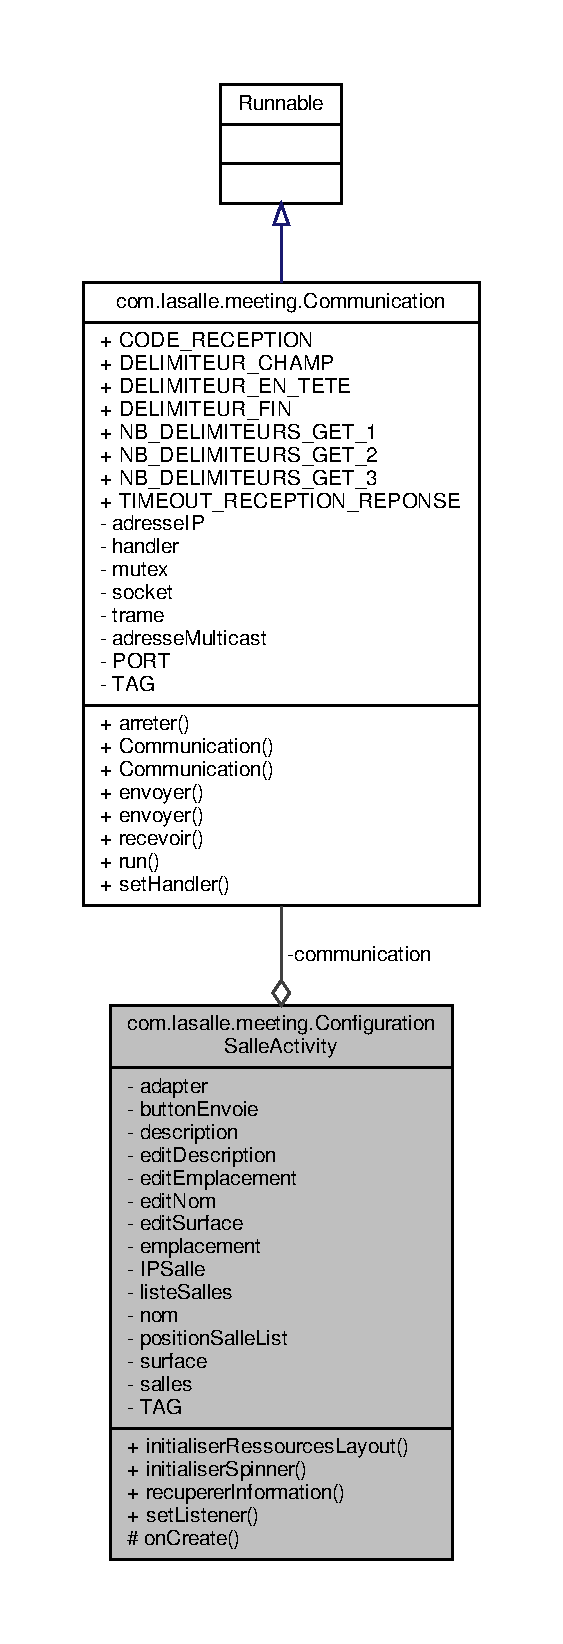
\includegraphics[height=550pt]{classcom_1_1lasalle_1_1meeting_1_1_configuration_salle_activity__coll__graph}
\end{center}
\end{figure}
\subsubsection*{Fonctions membres publiques}
\begin{DoxyCompactItemize}
\item 
void \hyperlink{classcom_1_1lasalle_1_1meeting_1_1_configuration_salle_activity_a24314b86f87df50bb933484d1d1435ac}{initialiser\+Ressources\+Layout} ()
\begin{DoxyCompactList}\small\item\em Récupère et initialise les widgets du layout activity\+\_\+configuration\+\_\+salle. \end{DoxyCompactList}\item 
void \hyperlink{classcom_1_1lasalle_1_1meeting_1_1_configuration_salle_activity_ac0b88ac36a5ee40988f3ee8fea7c54ee}{initialiser\+Spinner} ()
\begin{DoxyCompactList}\small\item\em initialise la vue \end{DoxyCompactList}\item 
void \hyperlink{classcom_1_1lasalle_1_1meeting_1_1_configuration_salle_activity_a6c5c3c9c513b13eb9182573732d392f5}{recuperer\+Information} ()
\begin{DoxyCompactList}\small\item\em recuepe et applique les informations mis dans les layouts \end{DoxyCompactList}\item 
void \hyperlink{classcom_1_1lasalle_1_1meeting_1_1_configuration_salle_activity_a8d3eea01718b9535c88caa796d8b6377}{set\+Listener} ()
\begin{DoxyCompactList}\small\item\em applique les listener sur les layouts approprié \end{DoxyCompactList}\end{DoxyCompactItemize}
\subsubsection*{Fonctions membres protégées}
\begin{DoxyCompactItemize}
\item 
void \hyperlink{classcom_1_1lasalle_1_1meeting_1_1_configuration_salle_activity_a202931e45bdc0f81c3f0518a6b28e712}{on\+Create} (Bundle saved\+Instance\+State)
\begin{DoxyCompactList}\small\item\em Méthode appelée à la création de l\textquotesingle{}activité \hyperlink{classcom_1_1lasalle_1_1meeting_1_1_configuration_salle_activity}{Configuration\+Salle\+Activity}. \end{DoxyCompactList}\end{DoxyCompactItemize}
\subsubsection*{Attributs privés}
\begin{DoxyCompactItemize}
\item 
Array\+Adapter$<$ String $>$ \hyperlink{classcom_1_1lasalle_1_1meeting_1_1_configuration_salle_activity_a168dba575f6638ba8c9081dad1b55a6e}{adapter}
\begin{DoxyCompactList}\small\item\em l\textquotesingle{}adaptateur \end{DoxyCompactList}\item 
Button \hyperlink{classcom_1_1lasalle_1_1meeting_1_1_configuration_salle_activity_a1222b15c71483d1b48ed0eb78724db91}{button\+Envoie}
\begin{DoxyCompactList}\small\item\em layout du bouton envoie \end{DoxyCompactList}\item 
\hyperlink{classcom_1_1lasalle_1_1meeting_1_1_communication}{Communication} \hyperlink{classcom_1_1lasalle_1_1meeting_1_1_configuration_salle_activity_a8ad9ee754954c8bc7d9c3f8313e48a2c}{communication} = null
\begin{DoxyCompactList}\small\item\em attribut permetant d\textquotesingle{}envoyer une requête \end{DoxyCompactList}\item 
String \hyperlink{classcom_1_1lasalle_1_1meeting_1_1_configuration_salle_activity_a2cdfb9a7b34f5d63e346a535411337cc}{description} =\char`\"{}\char`\"{}
\begin{DoxyCompactList}\small\item\em attribut de la description de la salle \end{DoxyCompactList}\item 
Edit\+Text \hyperlink{classcom_1_1lasalle_1_1meeting_1_1_configuration_salle_activity_a13e08adff1d4f5317a239a0eb9013bd6}{edit\+Description}
\begin{DoxyCompactList}\small\item\em layout récuperant la description donné \end{DoxyCompactList}\item 
Edit\+Text \hyperlink{classcom_1_1lasalle_1_1meeting_1_1_configuration_salle_activity_aed6844bdfcc65ccf7b9b9ca1960c6773}{edit\+Emplacement}
\begin{DoxyCompactList}\small\item\em layout récuperant l\textquotesingle{}emplacement donné \end{DoxyCompactList}\item 
Edit\+Text \hyperlink{classcom_1_1lasalle_1_1meeting_1_1_configuration_salle_activity_a79f6eb0127fb0182880b9f1eefda39c8}{edit\+Nom}
\begin{DoxyCompactList}\small\item\em layout récuperant le nom donné \end{DoxyCompactList}\item 
Edit\+Text \hyperlink{classcom_1_1lasalle_1_1meeting_1_1_configuration_salle_activity_a75bd76c0944c831ff00668299d8db929}{edit\+Surface}
\begin{DoxyCompactList}\small\item\em layout récuperant la surface donné \end{DoxyCompactList}\item 
String \hyperlink{classcom_1_1lasalle_1_1meeting_1_1_configuration_salle_activity_aeaee855a9fd72ad17519c287f2dcc322}{emplacement} =\char`\"{}\char`\"{}
\begin{DoxyCompactList}\small\item\em attribut de l\textquotesingle{}emplacement de la salle \end{DoxyCompactList}\item 
List$<$ String $>$ \hyperlink{classcom_1_1lasalle_1_1meeting_1_1_configuration_salle_activity_a74bb868ae39746bae6533c1735207abf}{I\+P\+Salle}
\begin{DoxyCompactList}\small\item\em les données traité \end{DoxyCompactList}\item 
Spinner \hyperlink{classcom_1_1lasalle_1_1meeting_1_1_configuration_salle_activity_ac1fa67c33882d1f181ba80a061ad097a}{liste\+Salles}
\begin{DoxyCompactList}\small\item\em la vue \end{DoxyCompactList}\item 
String \hyperlink{classcom_1_1lasalle_1_1meeting_1_1_configuration_salle_activity_ae7ae98c2c6e8e8d42260100ecc70aabc}{nom} =\char`\"{}\char`\"{}
\begin{DoxyCompactList}\small\item\em attribut du nom de la salle \end{DoxyCompactList}\item 
int \hyperlink{classcom_1_1lasalle_1_1meeting_1_1_configuration_salle_activity_ae76edfdd5b57cd474cccb830950f864a}{position\+Salle\+List} = 0
\begin{DoxyCompactList}\small\item\em position dans la vue \end{DoxyCompactList}\item 
String \hyperlink{classcom_1_1lasalle_1_1meeting_1_1_configuration_salle_activity_a3d27df453e9f461eb7402a8f69ca7ae1}{surface} =\char`\"{}\char`\"{}
\begin{DoxyCompactList}\small\item\em attribut de la surface de la salle \end{DoxyCompactList}\end{DoxyCompactItemize}
\subsubsection*{Attributs privés statiques}
\begin{DoxyCompactItemize}
\item 
static Vector$<$ \hyperlink{classcom_1_1lasalle_1_1meeting_1_1_salle}{Salle} $>$ \hyperlink{classcom_1_1lasalle_1_1meeting_1_1_configuration_salle_activity_afe3082468b9dd31ba0ec92e22bf27ab8}{salles}
\begin{DoxyCompactList}\small\item\em les données non traité \end{DoxyCompactList}\item 
static final String \hyperlink{classcom_1_1lasalle_1_1meeting_1_1_configuration_salle_activity_a55224a88c619aa44eb96c0febc3f1857}{T\+AG} = \char`\"{}Configuration\+Salle\+Activity\char`\"{}
\begin{DoxyCompactList}\small\item\em T\+AG utilisé pour les logs. \end{DoxyCompactList}\end{DoxyCompactItemize}


\subsubsection{Description détaillée}
Déclaration de la classe \hyperlink{classcom_1_1lasalle_1_1meeting_1_1_configuration_salle_activity}{Configuration\+Salle\+Activity}. 

Définition à la ligne \hyperlink{_configuration_salle_activity_8java_source_l00032}{32} du fichier \hyperlink{_configuration_salle_activity_8java_source}{Configuration\+Salle\+Activity.\+java}.



\subsubsection{Documentation des fonctions membres}
\mbox{\Hypertarget{classcom_1_1lasalle_1_1meeting_1_1_configuration_salle_activity_a24314b86f87df50bb933484d1d1435ac}\label{classcom_1_1lasalle_1_1meeting_1_1_configuration_salle_activity_a24314b86f87df50bb933484d1d1435ac}} 
\index{com\+::lasalle\+::meeting\+::\+Configuration\+Salle\+Activity@{com\+::lasalle\+::meeting\+::\+Configuration\+Salle\+Activity}!initialiser\+Ressources\+Layout@{initialiser\+Ressources\+Layout}}
\index{initialiser\+Ressources\+Layout@{initialiser\+Ressources\+Layout}!com\+::lasalle\+::meeting\+::\+Configuration\+Salle\+Activity@{com\+::lasalle\+::meeting\+::\+Configuration\+Salle\+Activity}}
\paragraph{\texorpdfstring{initialiser\+Ressources\+Layout()}{initialiserRessourcesLayout()}}
{\footnotesize\ttfamily void com.\+lasalle.\+meeting.\+Configuration\+Salle\+Activity.\+initialiser\+Ressources\+Layout (\begin{DoxyParamCaption}{ }\end{DoxyParamCaption})}



Récupère et initialise les widgets du layout activity\+\_\+configuration\+\_\+salle. 

\begin{DoxyReturn}{Renvoie}
void 
\end{DoxyReturn}


Définition à la ligne \hyperlink{_configuration_salle_activity_8java_source_l00084}{84} du fichier \hyperlink{_configuration_salle_activity_8java_source}{Configuration\+Salle\+Activity.\+java}.



Référencé par \hyperlink{_configuration_salle_activity_8java_source_l00066}{com.\+lasalle.\+meeting.\+Configuration\+Salle\+Activity.\+on\+Create()}.


\begin{DoxyCode}
00085     \{
00086         Log.d(\hyperlink{classcom_1_1lasalle_1_1meeting_1_1_configuration_salle_activity_a55224a88c619aa44eb96c0febc3f1857}{TAG}, \textcolor{stringliteral}{"initialiserRessourcesLayout()"});
00087 
00088         \hyperlink{classcom_1_1lasalle_1_1meeting_1_1_configuration_salle_activity_ac1fa67c33882d1f181ba80a061ad097a}{listeSalles} = (Spinner)findViewById(R.id.listeSalles);
00089         \hyperlink{classcom_1_1lasalle_1_1meeting_1_1_configuration_salle_activity_a79f6eb0127fb0182880b9f1eefda39c8}{editNom} = (EditText)findViewById(R.id.EditNom);
00090         \hyperlink{classcom_1_1lasalle_1_1meeting_1_1_configuration_salle_activity_aed6844bdfcc65ccf7b9b9ca1960c6773}{editEmplacement}= (EditText)findViewById(R.id.EditEmplacement);
00091         \hyperlink{classcom_1_1lasalle_1_1meeting_1_1_configuration_salle_activity_a13e08adff1d4f5317a239a0eb9013bd6}{editDescription}= (EditText)findViewById(R.id.EditDescription);
00092         \hyperlink{classcom_1_1lasalle_1_1meeting_1_1_configuration_salle_activity_a75bd76c0944c831ff00668299d8db929}{editSurface}= (EditText)findViewById(R.id.EditSurface);
00093         \hyperlink{classcom_1_1lasalle_1_1meeting_1_1_configuration_salle_activity_a1222b15c71483d1b48ed0eb78724db91}{buttonEnvoie}= (Button)findViewById(R.id.buttonEnvoie);
00094     \}
\end{DoxyCode}
\mbox{\Hypertarget{classcom_1_1lasalle_1_1meeting_1_1_configuration_salle_activity_ac0b88ac36a5ee40988f3ee8fea7c54ee}\label{classcom_1_1lasalle_1_1meeting_1_1_configuration_salle_activity_ac0b88ac36a5ee40988f3ee8fea7c54ee}} 
\index{com\+::lasalle\+::meeting\+::\+Configuration\+Salle\+Activity@{com\+::lasalle\+::meeting\+::\+Configuration\+Salle\+Activity}!initialiser\+Spinner@{initialiser\+Spinner}}
\index{initialiser\+Spinner@{initialiser\+Spinner}!com\+::lasalle\+::meeting\+::\+Configuration\+Salle\+Activity@{com\+::lasalle\+::meeting\+::\+Configuration\+Salle\+Activity}}
\paragraph{\texorpdfstring{initialiser\+Spinner()}{initialiserSpinner()}}
{\footnotesize\ttfamily void com.\+lasalle.\+meeting.\+Configuration\+Salle\+Activity.\+initialiser\+Spinner (\begin{DoxyParamCaption}{ }\end{DoxyParamCaption})}



initialise la vue 

\begin{DoxyReturn}{Renvoie}
void 
\end{DoxyReturn}


Définition à la ligne \hyperlink{_configuration_salle_activity_8java_source_l00100}{100} du fichier \hyperlink{_configuration_salle_activity_8java_source}{Configuration\+Salle\+Activity.\+java}.



Références \hyperlink{_main_activity_8java_source_l00470}{com.\+lasalle.\+meeting.\+Main\+Activity.\+get\+Mes\+Salles()}, et \hyperlink{_configuration_salle_activity_8java_source_l00042}{com.\+lasalle.\+meeting.\+Configuration\+Salle\+Activity.\+I\+P\+Salle}.



Référencé par \hyperlink{_configuration_salle_activity_8java_source_l00066}{com.\+lasalle.\+meeting.\+Configuration\+Salle\+Activity.\+on\+Create()}.


\begin{DoxyCode}
00101     \{
00102         Log.d(\hyperlink{classcom_1_1lasalle_1_1meeting_1_1_configuration_salle_activity_a55224a88c619aa44eb96c0febc3f1857}{TAG}, \textcolor{stringliteral}{"initialiserSpinner()"});
00103 
00104         \hyperlink{classcom_1_1lasalle_1_1meeting_1_1_configuration_salle_activity_a74bb868ae39746bae6533c1735207abf}{IPSalle} = \textcolor{keyword}{new} ArrayList<String>();
00105 
00106         \hyperlink{classcom_1_1lasalle_1_1meeting_1_1_configuration_salle_activity_afe3082468b9dd31ba0ec92e22bf27ab8}{salles} = MainActivity.getMesSalles();
00107 
00108         \textcolor{keywordflow}{for}(\textcolor{keywordtype}{int} i = 0; i < salles.size(); ++i)
00109         \{
00110             Log.d(\hyperlink{classcom_1_1lasalle_1_1meeting_1_1_configuration_salle_activity_a55224a88c619aa44eb96c0febc3f1857}{TAG}, \textcolor{stringliteral}{"Ajout adresse IP : "} + salles.elementAt(i).getAdresseIP());
00111             \hyperlink{classcom_1_1lasalle_1_1meeting_1_1_configuration_salle_activity_a74bb868ae39746bae6533c1735207abf}{IPSalle}.add(salles.elementAt(i).getAdresseIP());
00112         \}
00113 
00114         \hyperlink{classcom_1_1lasalle_1_1meeting_1_1_configuration_salle_activity_a168dba575f6638ba8c9081dad1b55a6e}{adapter} = \textcolor{keyword}{new} ArrayAdapter<String>(\textcolor{keyword}{this}, android.R.layout.simple\_spinner\_item, 
      \hyperlink{classcom_1_1lasalle_1_1meeting_1_1_configuration_salle_activity_a74bb868ae39746bae6533c1735207abf}{IPSalle});
00115         \hyperlink{classcom_1_1lasalle_1_1meeting_1_1_configuration_salle_activity_a168dba575f6638ba8c9081dad1b55a6e}{adapter}.setDropDownViewResource(android.R.layout.simple\_spinner\_dropdown\_item);
00116 
00117         \hyperlink{classcom_1_1lasalle_1_1meeting_1_1_configuration_salle_activity_ac1fa67c33882d1f181ba80a061ad097a}{listeSalles}.setAdapter(\hyperlink{classcom_1_1lasalle_1_1meeting_1_1_configuration_salle_activity_a168dba575f6638ba8c9081dad1b55a6e}{adapter});
00118 
00119         \hyperlink{classcom_1_1lasalle_1_1meeting_1_1_configuration_salle_activity_ac1fa67c33882d1f181ba80a061ad097a}{listeSalles}.setOnItemSelectedListener(\textcolor{keyword}{new} AdapterView.OnItemSelectedListener()
00120         \{
00121             @Override
00122             \textcolor{keyword}{public} \textcolor{keywordtype}{void} onItemSelected(AdapterView<?> arg0, View arg1, \textcolor{keywordtype}{int} position, \textcolor{keywordtype}{long} \textcolor{keywordtype}{id})
00123             \{
00124                 \hyperlink{classcom_1_1lasalle_1_1meeting_1_1_configuration_salle_activity_ae76edfdd5b57cd474cccb830950f864a}{positionSalleList} = position;
00125                 Log.d(\hyperlink{classcom_1_1lasalle_1_1meeting_1_1_configuration_salle_activity_a55224a88c619aa44eb96c0febc3f1857}{TAG}, \textcolor{stringliteral}{"position : "} + position + \textcolor{stringliteral}{" - "} + \textcolor{stringliteral}{"nom : "} + 
      \hyperlink{classcom_1_1lasalle_1_1meeting_1_1_configuration_salle_activity_a74bb868ae39746bae6533c1735207abf}{IPSalle}.get(position));
00126             \}
00127             @Override
00128             \textcolor{keyword}{public} \textcolor{keywordtype}{void} onNothingSelected(AdapterView<?> arg0)
00129             \{
00130             \}
00131         \});
00132     \}
\end{DoxyCode}
\mbox{\Hypertarget{classcom_1_1lasalle_1_1meeting_1_1_configuration_salle_activity_a202931e45bdc0f81c3f0518a6b28e712}\label{classcom_1_1lasalle_1_1meeting_1_1_configuration_salle_activity_a202931e45bdc0f81c3f0518a6b28e712}} 
\index{com\+::lasalle\+::meeting\+::\+Configuration\+Salle\+Activity@{com\+::lasalle\+::meeting\+::\+Configuration\+Salle\+Activity}!on\+Create@{on\+Create}}
\index{on\+Create@{on\+Create}!com\+::lasalle\+::meeting\+::\+Configuration\+Salle\+Activity@{com\+::lasalle\+::meeting\+::\+Configuration\+Salle\+Activity}}
\paragraph{\texorpdfstring{on\+Create()}{onCreate()}}
{\footnotesize\ttfamily void com.\+lasalle.\+meeting.\+Configuration\+Salle\+Activity.\+on\+Create (\begin{DoxyParamCaption}\item[{Bundle}]{saved\+Instance\+State }\end{DoxyParamCaption})\hspace{0.3cm}{\ttfamily [protected]}}



Méthode appelée à la création de l\textquotesingle{}activité \hyperlink{classcom_1_1lasalle_1_1meeting_1_1_configuration_salle_activity}{Configuration\+Salle\+Activity}. 


\begin{DoxyParams}{Paramètres}
{\em saved\+Instance\+State} & \\
\hline
\end{DoxyParams}
\begin{DoxyReturn}{Renvoie}
void 
\end{DoxyReturn}


Définition à la ligne \hyperlink{_configuration_salle_activity_8java_source_l00066}{66} du fichier \hyperlink{_configuration_salle_activity_8java_source}{Configuration\+Salle\+Activity.\+java}.



Références \hyperlink{_main_activity_8java_source_l00479}{com.\+lasalle.\+meeting.\+Main\+Activity.\+get\+Communication()}, \hyperlink{_configuration_salle_activity_8java_source_l00084}{com.\+lasalle.\+meeting.\+Configuration\+Salle\+Activity.\+initialiser\+Ressources\+Layout()}, \hyperlink{_configuration_salle_activity_8java_source_l00100}{com.\+lasalle.\+meeting.\+Configuration\+Salle\+Activity.\+initialiser\+Spinner()}, et \hyperlink{_configuration_salle_activity_8java_source_l00138}{com.\+lasalle.\+meeting.\+Configuration\+Salle\+Activity.\+set\+Listener()}.


\begin{DoxyCode}
00067     \{
00068         Log.d(\hyperlink{classcom_1_1lasalle_1_1meeting_1_1_configuration_salle_activity_a55224a88c619aa44eb96c0febc3f1857}{TAG}, \textcolor{stringliteral}{"onCreate()"});
00069 
00070         super.onCreate(savedInstanceState);
00071         setContentView(R.layout.activity\_configuration\_salle);
00072 
00073         \hyperlink{classcom_1_1lasalle_1_1meeting_1_1_configuration_salle_activity_a8ad9ee754954c8bc7d9c3f8313e48a2c}{communication} = MainActivity.getCommunication();
00074 
00075         \hyperlink{classcom_1_1lasalle_1_1meeting_1_1_configuration_salle_activity_a24314b86f87df50bb933484d1d1435ac}{initialiserRessourcesLayout}();
00076         \hyperlink{classcom_1_1lasalle_1_1meeting_1_1_configuration_salle_activity_ac0b88ac36a5ee40988f3ee8fea7c54ee}{initialiserSpinner}();
00077         \hyperlink{classcom_1_1lasalle_1_1meeting_1_1_configuration_salle_activity_a8d3eea01718b9535c88caa796d8b6377}{setListener}();
00078     \}
\end{DoxyCode}
\mbox{\Hypertarget{classcom_1_1lasalle_1_1meeting_1_1_configuration_salle_activity_a6c5c3c9c513b13eb9182573732d392f5}\label{classcom_1_1lasalle_1_1meeting_1_1_configuration_salle_activity_a6c5c3c9c513b13eb9182573732d392f5}} 
\index{com\+::lasalle\+::meeting\+::\+Configuration\+Salle\+Activity@{com\+::lasalle\+::meeting\+::\+Configuration\+Salle\+Activity}!recuperer\+Information@{recuperer\+Information}}
\index{recuperer\+Information@{recuperer\+Information}!com\+::lasalle\+::meeting\+::\+Configuration\+Salle\+Activity@{com\+::lasalle\+::meeting\+::\+Configuration\+Salle\+Activity}}
\paragraph{\texorpdfstring{recuperer\+Information()}{recupererInformation()}}
{\footnotesize\ttfamily void com.\+lasalle.\+meeting.\+Configuration\+Salle\+Activity.\+recuperer\+Information (\begin{DoxyParamCaption}{ }\end{DoxyParamCaption})}



recuepe et applique les informations mis dans les layouts 

\begin{DoxyReturn}{Renvoie}
void 
\end{DoxyReturn}


Définition à la ligne \hyperlink{_configuration_salle_activity_8java_source_l00164}{164} du fichier \hyperlink{_configuration_salle_activity_8java_source}{Configuration\+Salle\+Activity.\+java}.



Référencé par \hyperlink{_configuration_salle_activity_8java_source_l00138}{com.\+lasalle.\+meeting.\+Configuration\+Salle\+Activity.\+set\+Listener()}.


\begin{DoxyCode}
00165     \{
00166         Log.d(\hyperlink{classcom_1_1lasalle_1_1meeting_1_1_configuration_salle_activity_a55224a88c619aa44eb96c0febc3f1857}{TAG}, \textcolor{stringliteral}{"recupererInformation()"});
00167 
00168         \hyperlink{classcom_1_1lasalle_1_1meeting_1_1_configuration_salle_activity_ae7ae98c2c6e8e8d42260100ecc70aabc}{nom} = \hyperlink{classcom_1_1lasalle_1_1meeting_1_1_configuration_salle_activity_a79f6eb0127fb0182880b9f1eefda39c8}{editNom}.getText().toString();
00169         \hyperlink{classcom_1_1lasalle_1_1meeting_1_1_configuration_salle_activity_a2cdfb9a7b34f5d63e346a535411337cc}{description} = \hyperlink{classcom_1_1lasalle_1_1meeting_1_1_configuration_salle_activity_a13e08adff1d4f5317a239a0eb9013bd6}{editDescription}.getText().toString();
00170         \hyperlink{classcom_1_1lasalle_1_1meeting_1_1_configuration_salle_activity_aeaee855a9fd72ad17519c287f2dcc322}{emplacement} = \hyperlink{classcom_1_1lasalle_1_1meeting_1_1_configuration_salle_activity_aed6844bdfcc65ccf7b9b9ca1960c6773}{editEmplacement}.getText().toString();
00171         \hyperlink{classcom_1_1lasalle_1_1meeting_1_1_configuration_salle_activity_a3d27df453e9f461eb7402a8f69ca7ae1}{surface} = \hyperlink{classcom_1_1lasalle_1_1meeting_1_1_configuration_salle_activity_a75bd76c0944c831ff00668299d8db929}{editSurface}.getText().toString();
00172     \}
\end{DoxyCode}
\mbox{\Hypertarget{classcom_1_1lasalle_1_1meeting_1_1_configuration_salle_activity_a8d3eea01718b9535c88caa796d8b6377}\label{classcom_1_1lasalle_1_1meeting_1_1_configuration_salle_activity_a8d3eea01718b9535c88caa796d8b6377}} 
\index{com\+::lasalle\+::meeting\+::\+Configuration\+Salle\+Activity@{com\+::lasalle\+::meeting\+::\+Configuration\+Salle\+Activity}!set\+Listener@{set\+Listener}}
\index{set\+Listener@{set\+Listener}!com\+::lasalle\+::meeting\+::\+Configuration\+Salle\+Activity@{com\+::lasalle\+::meeting\+::\+Configuration\+Salle\+Activity}}
\paragraph{\texorpdfstring{set\+Listener()}{setListener()}}
{\footnotesize\ttfamily void com.\+lasalle.\+meeting.\+Configuration\+Salle\+Activity.\+set\+Listener (\begin{DoxyParamCaption}{ }\end{DoxyParamCaption})}



applique les listener sur les layouts approprié 

\begin{DoxyReturn}{Renvoie}
void 
\end{DoxyReturn}


Définition à la ligne \hyperlink{_configuration_salle_activity_8java_source_l00138}{138} du fichier \hyperlink{_configuration_salle_activity_8java_source}{Configuration\+Salle\+Activity.\+java}.



Références \hyperlink{_communication_8java_source_l00161}{com.\+lasalle.\+meeting.\+Communication.\+envoyer()}, et \hyperlink{_configuration_salle_activity_8java_source_l00164}{com.\+lasalle.\+meeting.\+Configuration\+Salle\+Activity.\+recuperer\+Information()}.



Référencé par \hyperlink{_configuration_salle_activity_8java_source_l00066}{com.\+lasalle.\+meeting.\+Configuration\+Salle\+Activity.\+on\+Create()}.


\begin{DoxyCode}
00139     \{
00140         Log.d(\hyperlink{classcom_1_1lasalle_1_1meeting_1_1_configuration_salle_activity_a55224a88c619aa44eb96c0febc3f1857}{TAG}, \textcolor{stringliteral}{"setListener()"});
00141 
00142         \hyperlink{classcom_1_1lasalle_1_1meeting_1_1_configuration_salle_activity_a1222b15c71483d1b48ed0eb78724db91}{buttonEnvoie}.setOnClickListener(
00143             \textcolor{keyword}{new} View.OnClickListener()
00144             \{
00145                 @Override
00146                 \textcolor{keyword}{public} \textcolor{keywordtype}{void} onClick(View v)
00147                 \{
00148                     \hyperlink{classcom_1_1lasalle_1_1meeting_1_1_configuration_salle_activity_a6c5c3c9c513b13eb9182573732d392f5}{recupererInformation}();
00149 
00150                     Log.d(\hyperlink{classcom_1_1lasalle_1_1meeting_1_1_configuration_salle_activity_a55224a88c619aa44eb96c0febc3f1857}{TAG},\textcolor{stringliteral}{"trame : $SET;1;"} + \hyperlink{classcom_1_1lasalle_1_1meeting_1_1_configuration_salle_activity_ae7ae98c2c6e8e8d42260100ecc70aabc}{nom} + \textcolor{stringliteral}{";"} + \hyperlink{classcom_1_1lasalle_1_1meeting_1_1_configuration_salle_activity_a2cdfb9a7b34f5d63e346a535411337cc}{description} + \textcolor{stringliteral}{";"} + 
      \hyperlink{classcom_1_1lasalle_1_1meeting_1_1_configuration_salle_activity_aeaee855a9fd72ad17519c287f2dcc322}{emplacement} + \textcolor{stringliteral}{";"} + \hyperlink{classcom_1_1lasalle_1_1meeting_1_1_configuration_salle_activity_a3d27df453e9f461eb7402a8f69ca7ae1}{surface} + \textcolor{stringliteral}{"\(\backslash\)r\(\backslash\)n"} + \hyperlink{classcom_1_1lasalle_1_1meeting_1_1_configuration_salle_activity_a74bb868ae39746bae6533c1735207abf}{IPSalle}.get(
      \hyperlink{classcom_1_1lasalle_1_1meeting_1_1_configuration_salle_activity_ae76edfdd5b57cd474cccb830950f864a}{positionSalleList}));
00151                     \textcolor{keywordflow}{if}(\hyperlink{classcom_1_1lasalle_1_1meeting_1_1_configuration_salle_activity_a8ad9ee754954c8bc7d9c3f8313e48a2c}{communication} != null)
00152                     \{
00153                         \hyperlink{classcom_1_1lasalle_1_1meeting_1_1_configuration_salle_activity_a8ad9ee754954c8bc7d9c3f8313e48a2c}{communication}.\hyperlink{classcom_1_1lasalle_1_1meeting_1_1_communication_a1566200ca56ba63eec13d0ce37e6c7ee}{envoyer}(\textcolor{stringliteral}{"$SET;1;"} + 
      \hyperlink{classcom_1_1lasalle_1_1meeting_1_1_configuration_salle_activity_ae7ae98c2c6e8e8d42260100ecc70aabc}{nom} + \textcolor{stringliteral}{";"} + \hyperlink{classcom_1_1lasalle_1_1meeting_1_1_configuration_salle_activity_a2cdfb9a7b34f5d63e346a535411337cc}{description} + \textcolor{stringliteral}{";"} + \hyperlink{classcom_1_1lasalle_1_1meeting_1_1_configuration_salle_activity_aeaee855a9fd72ad17519c287f2dcc322}{emplacement} + \textcolor{stringliteral}{";"} + 
      \hyperlink{classcom_1_1lasalle_1_1meeting_1_1_configuration_salle_activity_a3d27df453e9f461eb7402a8f69ca7ae1}{surface} + \textcolor{stringliteral}{"\(\backslash\)r\(\backslash\)n"}, \hyperlink{classcom_1_1lasalle_1_1meeting_1_1_configuration_salle_activity_a74bb868ae39746bae6533c1735207abf}{IPSalle}.get(\hyperlink{classcom_1_1lasalle_1_1meeting_1_1_configuration_salle_activity_ae76edfdd5b57cd474cccb830950f864a}{positionSalleList}));
00154                     \}
00155                 \}
00156             \}
00157         );
00158     \}
\end{DoxyCode}


\subsubsection{Documentation des données membres}
\mbox{\Hypertarget{classcom_1_1lasalle_1_1meeting_1_1_configuration_salle_activity_a168dba575f6638ba8c9081dad1b55a6e}\label{classcom_1_1lasalle_1_1meeting_1_1_configuration_salle_activity_a168dba575f6638ba8c9081dad1b55a6e}} 
\index{com\+::lasalle\+::meeting\+::\+Configuration\+Salle\+Activity@{com\+::lasalle\+::meeting\+::\+Configuration\+Salle\+Activity}!adapter@{adapter}}
\index{adapter@{adapter}!com\+::lasalle\+::meeting\+::\+Configuration\+Salle\+Activity@{com\+::lasalle\+::meeting\+::\+Configuration\+Salle\+Activity}}
\paragraph{\texorpdfstring{adapter}{adapter}}
{\footnotesize\ttfamily Array\+Adapter$<$String$>$ com.\+lasalle.\+meeting.\+Configuration\+Salle\+Activity.\+adapter\hspace{0.3cm}{\ttfamily [private]}}



l\textquotesingle{}adaptateur 



Définition à la ligne \hyperlink{_configuration_salle_activity_8java_source_l00043}{43} du fichier \hyperlink{_configuration_salle_activity_8java_source}{Configuration\+Salle\+Activity.\+java}.

\mbox{\Hypertarget{classcom_1_1lasalle_1_1meeting_1_1_configuration_salle_activity_a1222b15c71483d1b48ed0eb78724db91}\label{classcom_1_1lasalle_1_1meeting_1_1_configuration_salle_activity_a1222b15c71483d1b48ed0eb78724db91}} 
\index{com\+::lasalle\+::meeting\+::\+Configuration\+Salle\+Activity@{com\+::lasalle\+::meeting\+::\+Configuration\+Salle\+Activity}!button\+Envoie@{button\+Envoie}}
\index{button\+Envoie@{button\+Envoie}!com\+::lasalle\+::meeting\+::\+Configuration\+Salle\+Activity@{com\+::lasalle\+::meeting\+::\+Configuration\+Salle\+Activity}}
\paragraph{\texorpdfstring{button\+Envoie}{buttonEnvoie}}
{\footnotesize\ttfamily Button com.\+lasalle.\+meeting.\+Configuration\+Salle\+Activity.\+button\+Envoie\hspace{0.3cm}{\ttfamily [private]}}



layout du bouton envoie 



Définition à la ligne \hyperlink{_configuration_salle_activity_8java_source_l00058}{58} du fichier \hyperlink{_configuration_salle_activity_8java_source}{Configuration\+Salle\+Activity.\+java}.

\mbox{\Hypertarget{classcom_1_1lasalle_1_1meeting_1_1_configuration_salle_activity_a8ad9ee754954c8bc7d9c3f8313e48a2c}\label{classcom_1_1lasalle_1_1meeting_1_1_configuration_salle_activity_a8ad9ee754954c8bc7d9c3f8313e48a2c}} 
\index{com\+::lasalle\+::meeting\+::\+Configuration\+Salle\+Activity@{com\+::lasalle\+::meeting\+::\+Configuration\+Salle\+Activity}!communication@{communication}}
\index{communication@{communication}!com\+::lasalle\+::meeting\+::\+Configuration\+Salle\+Activity@{com\+::lasalle\+::meeting\+::\+Configuration\+Salle\+Activity}}
\paragraph{\texorpdfstring{communication}{communication}}
{\footnotesize\ttfamily \hyperlink{classcom_1_1lasalle_1_1meeting_1_1_communication}{Communication} com.\+lasalle.\+meeting.\+Configuration\+Salle\+Activity.\+communication = null\hspace{0.3cm}{\ttfamily [private]}}



attribut permetant d\textquotesingle{}envoyer une requête 



Définition à la ligne \hyperlink{_configuration_salle_activity_8java_source_l00045}{45} du fichier \hyperlink{_configuration_salle_activity_8java_source}{Configuration\+Salle\+Activity.\+java}.

\mbox{\Hypertarget{classcom_1_1lasalle_1_1meeting_1_1_configuration_salle_activity_a2cdfb9a7b34f5d63e346a535411337cc}\label{classcom_1_1lasalle_1_1meeting_1_1_configuration_salle_activity_a2cdfb9a7b34f5d63e346a535411337cc}} 
\index{com\+::lasalle\+::meeting\+::\+Configuration\+Salle\+Activity@{com\+::lasalle\+::meeting\+::\+Configuration\+Salle\+Activity}!description@{description}}
\index{description@{description}!com\+::lasalle\+::meeting\+::\+Configuration\+Salle\+Activity@{com\+::lasalle\+::meeting\+::\+Configuration\+Salle\+Activity}}
\paragraph{\texorpdfstring{description}{description}}
{\footnotesize\ttfamily String com.\+lasalle.\+meeting.\+Configuration\+Salle\+Activity.\+description =\char`\"{}\char`\"{}\hspace{0.3cm}{\ttfamily [private]}}



attribut de la description de la salle 



Définition à la ligne \hyperlink{_configuration_salle_activity_8java_source_l00049}{49} du fichier \hyperlink{_configuration_salle_activity_8java_source}{Configuration\+Salle\+Activity.\+java}.

\mbox{\Hypertarget{classcom_1_1lasalle_1_1meeting_1_1_configuration_salle_activity_a13e08adff1d4f5317a239a0eb9013bd6}\label{classcom_1_1lasalle_1_1meeting_1_1_configuration_salle_activity_a13e08adff1d4f5317a239a0eb9013bd6}} 
\index{com\+::lasalle\+::meeting\+::\+Configuration\+Salle\+Activity@{com\+::lasalle\+::meeting\+::\+Configuration\+Salle\+Activity}!edit\+Description@{edit\+Description}}
\index{edit\+Description@{edit\+Description}!com\+::lasalle\+::meeting\+::\+Configuration\+Salle\+Activity@{com\+::lasalle\+::meeting\+::\+Configuration\+Salle\+Activity}}
\paragraph{\texorpdfstring{edit\+Description}{editDescription}}
{\footnotesize\ttfamily Edit\+Text com.\+lasalle.\+meeting.\+Configuration\+Salle\+Activity.\+edit\+Description\hspace{0.3cm}{\ttfamily [private]}}



layout récuperant la description donné 



Définition à la ligne \hyperlink{_configuration_salle_activity_8java_source_l00056}{56} du fichier \hyperlink{_configuration_salle_activity_8java_source}{Configuration\+Salle\+Activity.\+java}.

\mbox{\Hypertarget{classcom_1_1lasalle_1_1meeting_1_1_configuration_salle_activity_aed6844bdfcc65ccf7b9b9ca1960c6773}\label{classcom_1_1lasalle_1_1meeting_1_1_configuration_salle_activity_aed6844bdfcc65ccf7b9b9ca1960c6773}} 
\index{com\+::lasalle\+::meeting\+::\+Configuration\+Salle\+Activity@{com\+::lasalle\+::meeting\+::\+Configuration\+Salle\+Activity}!edit\+Emplacement@{edit\+Emplacement}}
\index{edit\+Emplacement@{edit\+Emplacement}!com\+::lasalle\+::meeting\+::\+Configuration\+Salle\+Activity@{com\+::lasalle\+::meeting\+::\+Configuration\+Salle\+Activity}}
\paragraph{\texorpdfstring{edit\+Emplacement}{editEmplacement}}
{\footnotesize\ttfamily Edit\+Text com.\+lasalle.\+meeting.\+Configuration\+Salle\+Activity.\+edit\+Emplacement\hspace{0.3cm}{\ttfamily [private]}}



layout récuperant l\textquotesingle{}emplacement donné 



Définition à la ligne \hyperlink{_configuration_salle_activity_8java_source_l00055}{55} du fichier \hyperlink{_configuration_salle_activity_8java_source}{Configuration\+Salle\+Activity.\+java}.

\mbox{\Hypertarget{classcom_1_1lasalle_1_1meeting_1_1_configuration_salle_activity_a79f6eb0127fb0182880b9f1eefda39c8}\label{classcom_1_1lasalle_1_1meeting_1_1_configuration_salle_activity_a79f6eb0127fb0182880b9f1eefda39c8}} 
\index{com\+::lasalle\+::meeting\+::\+Configuration\+Salle\+Activity@{com\+::lasalle\+::meeting\+::\+Configuration\+Salle\+Activity}!edit\+Nom@{edit\+Nom}}
\index{edit\+Nom@{edit\+Nom}!com\+::lasalle\+::meeting\+::\+Configuration\+Salle\+Activity@{com\+::lasalle\+::meeting\+::\+Configuration\+Salle\+Activity}}
\paragraph{\texorpdfstring{edit\+Nom}{editNom}}
{\footnotesize\ttfamily Edit\+Text com.\+lasalle.\+meeting.\+Configuration\+Salle\+Activity.\+edit\+Nom\hspace{0.3cm}{\ttfamily [private]}}



layout récuperant le nom donné 

Ressources layout activity\+\_\+main 

Définition à la ligne \hyperlink{_configuration_salle_activity_8java_source_l00054}{54} du fichier \hyperlink{_configuration_salle_activity_8java_source}{Configuration\+Salle\+Activity.\+java}.

\mbox{\Hypertarget{classcom_1_1lasalle_1_1meeting_1_1_configuration_salle_activity_a75bd76c0944c831ff00668299d8db929}\label{classcom_1_1lasalle_1_1meeting_1_1_configuration_salle_activity_a75bd76c0944c831ff00668299d8db929}} 
\index{com\+::lasalle\+::meeting\+::\+Configuration\+Salle\+Activity@{com\+::lasalle\+::meeting\+::\+Configuration\+Salle\+Activity}!edit\+Surface@{edit\+Surface}}
\index{edit\+Surface@{edit\+Surface}!com\+::lasalle\+::meeting\+::\+Configuration\+Salle\+Activity@{com\+::lasalle\+::meeting\+::\+Configuration\+Salle\+Activity}}
\paragraph{\texorpdfstring{edit\+Surface}{editSurface}}
{\footnotesize\ttfamily Edit\+Text com.\+lasalle.\+meeting.\+Configuration\+Salle\+Activity.\+edit\+Surface\hspace{0.3cm}{\ttfamily [private]}}



layout récuperant la surface donné 



Définition à la ligne \hyperlink{_configuration_salle_activity_8java_source_l00057}{57} du fichier \hyperlink{_configuration_salle_activity_8java_source}{Configuration\+Salle\+Activity.\+java}.

\mbox{\Hypertarget{classcom_1_1lasalle_1_1meeting_1_1_configuration_salle_activity_aeaee855a9fd72ad17519c287f2dcc322}\label{classcom_1_1lasalle_1_1meeting_1_1_configuration_salle_activity_aeaee855a9fd72ad17519c287f2dcc322}} 
\index{com\+::lasalle\+::meeting\+::\+Configuration\+Salle\+Activity@{com\+::lasalle\+::meeting\+::\+Configuration\+Salle\+Activity}!emplacement@{emplacement}}
\index{emplacement@{emplacement}!com\+::lasalle\+::meeting\+::\+Configuration\+Salle\+Activity@{com\+::lasalle\+::meeting\+::\+Configuration\+Salle\+Activity}}
\paragraph{\texorpdfstring{emplacement}{emplacement}}
{\footnotesize\ttfamily String com.\+lasalle.\+meeting.\+Configuration\+Salle\+Activity.\+emplacement =\char`\"{}\char`\"{}\hspace{0.3cm}{\ttfamily [private]}}



attribut de l\textquotesingle{}emplacement de la salle 



Définition à la ligne \hyperlink{_configuration_salle_activity_8java_source_l00048}{48} du fichier \hyperlink{_configuration_salle_activity_8java_source}{Configuration\+Salle\+Activity.\+java}.

\mbox{\Hypertarget{classcom_1_1lasalle_1_1meeting_1_1_configuration_salle_activity_a74bb868ae39746bae6533c1735207abf}\label{classcom_1_1lasalle_1_1meeting_1_1_configuration_salle_activity_a74bb868ae39746bae6533c1735207abf}} 
\index{com\+::lasalle\+::meeting\+::\+Configuration\+Salle\+Activity@{com\+::lasalle\+::meeting\+::\+Configuration\+Salle\+Activity}!I\+P\+Salle@{I\+P\+Salle}}
\index{I\+P\+Salle@{I\+P\+Salle}!com\+::lasalle\+::meeting\+::\+Configuration\+Salle\+Activity@{com\+::lasalle\+::meeting\+::\+Configuration\+Salle\+Activity}}
\paragraph{\texorpdfstring{I\+P\+Salle}{IPSalle}}
{\footnotesize\ttfamily List$<$String$>$ com.\+lasalle.\+meeting.\+Configuration\+Salle\+Activity.\+I\+P\+Salle\hspace{0.3cm}{\ttfamily [private]}}



les données traité 



Définition à la ligne \hyperlink{_configuration_salle_activity_8java_source_l00042}{42} du fichier \hyperlink{_configuration_salle_activity_8java_source}{Configuration\+Salle\+Activity.\+java}.



Référencé par \hyperlink{_configuration_salle_activity_8java_source_l00100}{com.\+lasalle.\+meeting.\+Configuration\+Salle\+Activity.\+initialiser\+Spinner()}.

\mbox{\Hypertarget{classcom_1_1lasalle_1_1meeting_1_1_configuration_salle_activity_ac1fa67c33882d1f181ba80a061ad097a}\label{classcom_1_1lasalle_1_1meeting_1_1_configuration_salle_activity_ac1fa67c33882d1f181ba80a061ad097a}} 
\index{com\+::lasalle\+::meeting\+::\+Configuration\+Salle\+Activity@{com\+::lasalle\+::meeting\+::\+Configuration\+Salle\+Activity}!liste\+Salles@{liste\+Salles}}
\index{liste\+Salles@{liste\+Salles}!com\+::lasalle\+::meeting\+::\+Configuration\+Salle\+Activity@{com\+::lasalle\+::meeting\+::\+Configuration\+Salle\+Activity}}
\paragraph{\texorpdfstring{liste\+Salles}{listeSalles}}
{\footnotesize\ttfamily Spinner com.\+lasalle.\+meeting.\+Configuration\+Salle\+Activity.\+liste\+Salles\hspace{0.3cm}{\ttfamily [private]}}



la vue 

Attributs 

Définition à la ligne \hyperlink{_configuration_salle_activity_8java_source_l00041}{41} du fichier \hyperlink{_configuration_salle_activity_8java_source}{Configuration\+Salle\+Activity.\+java}.

\mbox{\Hypertarget{classcom_1_1lasalle_1_1meeting_1_1_configuration_salle_activity_ae7ae98c2c6e8e8d42260100ecc70aabc}\label{classcom_1_1lasalle_1_1meeting_1_1_configuration_salle_activity_ae7ae98c2c6e8e8d42260100ecc70aabc}} 
\index{com\+::lasalle\+::meeting\+::\+Configuration\+Salle\+Activity@{com\+::lasalle\+::meeting\+::\+Configuration\+Salle\+Activity}!nom@{nom}}
\index{nom@{nom}!com\+::lasalle\+::meeting\+::\+Configuration\+Salle\+Activity@{com\+::lasalle\+::meeting\+::\+Configuration\+Salle\+Activity}}
\paragraph{\texorpdfstring{nom}{nom}}
{\footnotesize\ttfamily String com.\+lasalle.\+meeting.\+Configuration\+Salle\+Activity.\+nom =\char`\"{}\char`\"{}\hspace{0.3cm}{\ttfamily [private]}}



attribut du nom de la salle 



Définition à la ligne \hyperlink{_configuration_salle_activity_8java_source_l00047}{47} du fichier \hyperlink{_configuration_salle_activity_8java_source}{Configuration\+Salle\+Activity.\+java}.

\mbox{\Hypertarget{classcom_1_1lasalle_1_1meeting_1_1_configuration_salle_activity_ae76edfdd5b57cd474cccb830950f864a}\label{classcom_1_1lasalle_1_1meeting_1_1_configuration_salle_activity_ae76edfdd5b57cd474cccb830950f864a}} 
\index{com\+::lasalle\+::meeting\+::\+Configuration\+Salle\+Activity@{com\+::lasalle\+::meeting\+::\+Configuration\+Salle\+Activity}!position\+Salle\+List@{position\+Salle\+List}}
\index{position\+Salle\+List@{position\+Salle\+List}!com\+::lasalle\+::meeting\+::\+Configuration\+Salle\+Activity@{com\+::lasalle\+::meeting\+::\+Configuration\+Salle\+Activity}}
\paragraph{\texorpdfstring{position\+Salle\+List}{positionSalleList}}
{\footnotesize\ttfamily int com.\+lasalle.\+meeting.\+Configuration\+Salle\+Activity.\+position\+Salle\+List = 0\hspace{0.3cm}{\ttfamily [private]}}



position dans la vue 



Définition à la ligne \hyperlink{_configuration_salle_activity_8java_source_l00046}{46} du fichier \hyperlink{_configuration_salle_activity_8java_source}{Configuration\+Salle\+Activity.\+java}.

\mbox{\Hypertarget{classcom_1_1lasalle_1_1meeting_1_1_configuration_salle_activity_afe3082468b9dd31ba0ec92e22bf27ab8}\label{classcom_1_1lasalle_1_1meeting_1_1_configuration_salle_activity_afe3082468b9dd31ba0ec92e22bf27ab8}} 
\index{com\+::lasalle\+::meeting\+::\+Configuration\+Salle\+Activity@{com\+::lasalle\+::meeting\+::\+Configuration\+Salle\+Activity}!salles@{salles}}
\index{salles@{salles}!com\+::lasalle\+::meeting\+::\+Configuration\+Salle\+Activity@{com\+::lasalle\+::meeting\+::\+Configuration\+Salle\+Activity}}
\paragraph{\texorpdfstring{salles}{salles}}
{\footnotesize\ttfamily Vector$<$\hyperlink{classcom_1_1lasalle_1_1meeting_1_1_salle}{Salle}$>$ com.\+lasalle.\+meeting.\+Configuration\+Salle\+Activity.\+salles\hspace{0.3cm}{\ttfamily [static]}, {\ttfamily [private]}}



les données non traité 



Définition à la ligne \hyperlink{_configuration_salle_activity_8java_source_l00044}{44} du fichier \hyperlink{_configuration_salle_activity_8java_source}{Configuration\+Salle\+Activity.\+java}.

\mbox{\Hypertarget{classcom_1_1lasalle_1_1meeting_1_1_configuration_salle_activity_a3d27df453e9f461eb7402a8f69ca7ae1}\label{classcom_1_1lasalle_1_1meeting_1_1_configuration_salle_activity_a3d27df453e9f461eb7402a8f69ca7ae1}} 
\index{com\+::lasalle\+::meeting\+::\+Configuration\+Salle\+Activity@{com\+::lasalle\+::meeting\+::\+Configuration\+Salle\+Activity}!surface@{surface}}
\index{surface@{surface}!com\+::lasalle\+::meeting\+::\+Configuration\+Salle\+Activity@{com\+::lasalle\+::meeting\+::\+Configuration\+Salle\+Activity}}
\paragraph{\texorpdfstring{surface}{surface}}
{\footnotesize\ttfamily String com.\+lasalle.\+meeting.\+Configuration\+Salle\+Activity.\+surface =\char`\"{}\char`\"{}\hspace{0.3cm}{\ttfamily [private]}}



attribut de la surface de la salle 



Définition à la ligne \hyperlink{_configuration_salle_activity_8java_source_l00050}{50} du fichier \hyperlink{_configuration_salle_activity_8java_source}{Configuration\+Salle\+Activity.\+java}.

\mbox{\Hypertarget{classcom_1_1lasalle_1_1meeting_1_1_configuration_salle_activity_a55224a88c619aa44eb96c0febc3f1857}\label{classcom_1_1lasalle_1_1meeting_1_1_configuration_salle_activity_a55224a88c619aa44eb96c0febc3f1857}} 
\index{com\+::lasalle\+::meeting\+::\+Configuration\+Salle\+Activity@{com\+::lasalle\+::meeting\+::\+Configuration\+Salle\+Activity}!T\+AG@{T\+AG}}
\index{T\+AG@{T\+AG}!com\+::lasalle\+::meeting\+::\+Configuration\+Salle\+Activity@{com\+::lasalle\+::meeting\+::\+Configuration\+Salle\+Activity}}
\paragraph{\texorpdfstring{T\+AG}{TAG}}
{\footnotesize\ttfamily final String com.\+lasalle.\+meeting.\+Configuration\+Salle\+Activity.\+T\+AG = \char`\"{}Configuration\+Salle\+Activity\char`\"{}\hspace{0.3cm}{\ttfamily [static]}, {\ttfamily [private]}}



T\+AG utilisé pour les logs. 

Constantes 

Définition à la ligne \hyperlink{_configuration_salle_activity_8java_source_l00037}{37} du fichier \hyperlink{_configuration_salle_activity_8java_source}{Configuration\+Salle\+Activity.\+java}.



La documentation de cette classe a été générée à partir du fichier suivant \+:\begin{DoxyCompactItemize}
\item 
\hyperlink{_configuration_salle_activity_8java}{Configuration\+Salle\+Activity.\+java}\end{DoxyCompactItemize}

\hypertarget{classcom_1_1lasalle_1_1meeting_1_1_main_activity}{}\subsection{Référence de la classe com.\+lasalle.\+meeting.\+Main\+Activity}
\label{classcom_1_1lasalle_1_1meeting_1_1_main_activity}\index{com.\+lasalle.\+meeting.\+Main\+Activity@{com.\+lasalle.\+meeting.\+Main\+Activity}}


Déclaration de la classe \hyperlink{classcom_1_1lasalle_1_1meeting_1_1_main_activity}{Main\+Activity}.  




Graphe de collaboration de com.\+lasalle.\+meeting.\+Main\+Activity\+:
\nopagebreak
\begin{figure}[H]
\begin{center}
\leavevmode
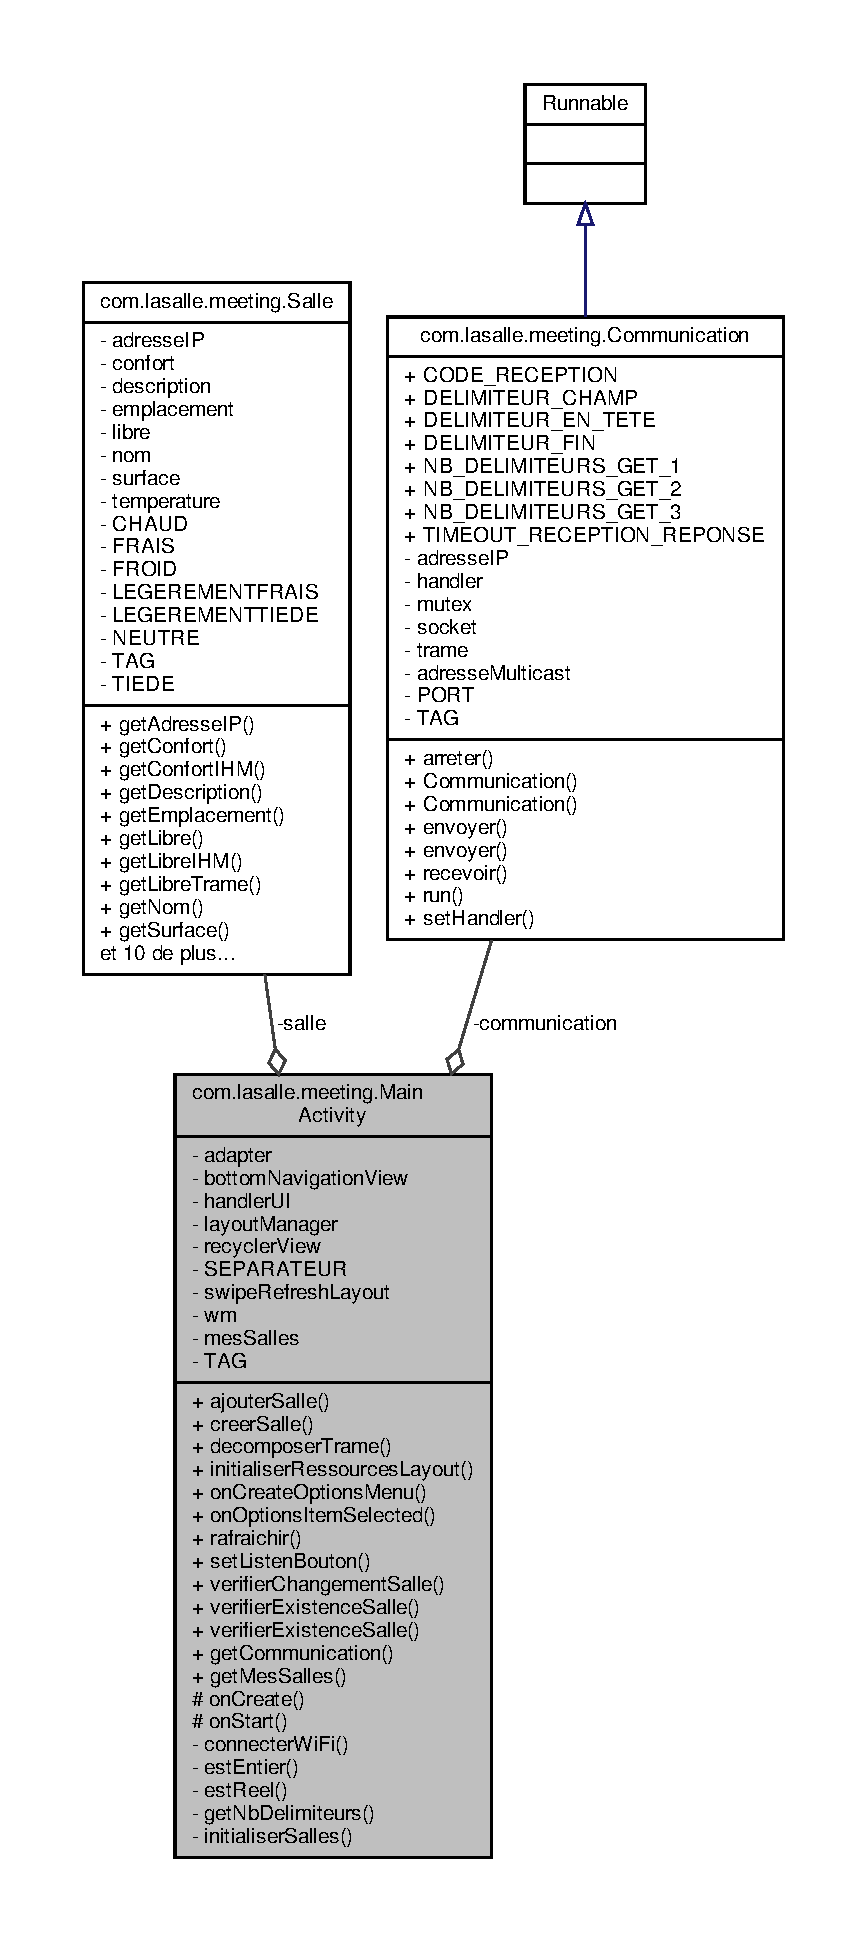
\includegraphics[height=550pt]{classcom_1_1lasalle_1_1meeting_1_1_main_activity__coll__graph}
\end{center}
\end{figure}
\subsubsection*{Fonctions membres publiques}
\begin{DoxyCompactItemize}
\item 
void \hyperlink{classcom_1_1lasalle_1_1meeting_1_1_main_activity_a8fded0b03a19faea1b0e735af1aa52ca}{ajouter\+Salle} (\hyperlink{classcom_1_1lasalle_1_1meeting_1_1_salle}{Salle} ma\+Salle)
\begin{DoxyCompactList}\small\item\em ajoute une salle au vecteur (mes\+Salles) \end{DoxyCompactList}\item 
\hyperlink{classcom_1_1lasalle_1_1meeting_1_1_salle}{Salle} \hyperlink{classcom_1_1lasalle_1_1meeting_1_1_main_activity_a882bcd3e88633b5190d60625bb70dd43}{creer\+Salle} (String\mbox{[}$\,$\mbox{]} trame\+Decompose, String adresse\+IP)
\begin{DoxyCompactList}\small\item\em créer une salle a partir de la trame \end{DoxyCompactList}\item 
String \mbox{[}$\,$\mbox{]} \hyperlink{classcom_1_1lasalle_1_1meeting_1_1_main_activity_ab9a644c245dafa25dc2ef9d099565425}{decomposer\+Trame} (String trame)
\begin{DoxyCompactList}\small\item\em découpe la trame \end{DoxyCompactList}\item 
void \hyperlink{classcom_1_1lasalle_1_1meeting_1_1_main_activity_a2622b1b85884f9d66038adfc162b2c30}{initialiser\+Ressources\+Layout} ()
\begin{DoxyCompactList}\small\item\em Récupère et initialise les widgets du layout activity\+\_\+main. \end{DoxyCompactList}\item 
boolean \hyperlink{classcom_1_1lasalle_1_1meeting_1_1_main_activity_a2ea2affb4c84cb17d1bef20c47421d15}{on\+Create\+Options\+Menu} (Menu menu)
\begin{DoxyCompactList}\small\item\em Méthode appelée au démarrage de l\textquotesingle{}activité \hyperlink{classcom_1_1lasalle_1_1meeting_1_1_main_activity}{Main\+Activity}. \end{DoxyCompactList}\item 
boolean \hyperlink{classcom_1_1lasalle_1_1meeting_1_1_main_activity_aa75ab3607c240fd26857f7eb6314e8bb}{on\+Options\+Item\+Selected} (Menu\+Item item)
\begin{DoxyCompactList}\small\item\em Méthode appelée quand on appuye sur boutons du menu. \end{DoxyCompactList}\item 
void \hyperlink{classcom_1_1lasalle_1_1meeting_1_1_main_activity_a58c77ea2af56877f661e85dcfd3f1299}{rafraichir} (Vector$<$ \hyperlink{classcom_1_1lasalle_1_1meeting_1_1_salle}{Salle} $>$ \hyperlink{classcom_1_1lasalle_1_1meeting_1_1_main_activity_ab13e34516d877abc3ba937505b441979}{mes\+Salles})
\begin{DoxyCompactList}\small\item\em rafraichis mon affichage \end{DoxyCompactList}\item 
void \hyperlink{classcom_1_1lasalle_1_1meeting_1_1_main_activity_a6bd5bed490e4679df4c4edbb0ce9a4cc}{set\+Listen\+Bouton} ()
\begin{DoxyCompactList}\small\item\em applique les listener sur les layouts approprié \end{DoxyCompactList}\item 
boolean \hyperlink{classcom_1_1lasalle_1_1meeting_1_1_main_activity_a1502e68ede2683ced61843887ca63963}{verifier\+Changement\+Salle} (\hyperlink{classcom_1_1lasalle_1_1meeting_1_1_salle}{Salle} ma\+Salle, int position\+Meme\+Salle)
\begin{DoxyCompactList}\small\item\em Vérifie que la salle n\textquotesingle{}est pas different que dans le vecteur, r\textquotesingle{}envoye true si il y a eu une modifiaction, r\textquotesingle{}envoye false si il y en a pas eux. \end{DoxyCompactList}\item 
int \hyperlink{classcom_1_1lasalle_1_1meeting_1_1_main_activity_ad0924169264a808e34a20c406efe0db2}{verifier\+Existence\+Salle} (\hyperlink{classcom_1_1lasalle_1_1meeting_1_1_salle}{Salle} ma\+Salle)
\begin{DoxyCompactList}\small\item\em verifie que la salle n\textquotesingle{}exisite pas déjà dans le vecteur, r\textquotesingle{}envoye -\/1 si il n\textquotesingle{}en existe pas, r\textquotesingle{}envoye la position de la salle dans le vecteur si il existe \end{DoxyCompactList}\item 
int \hyperlink{classcom_1_1lasalle_1_1meeting_1_1_main_activity_ac505af5465f0d95b1232acb745c86a08}{verifier\+Existence\+Salle} (String adresse\+IP)
\end{DoxyCompactItemize}
\subsubsection*{Fonctions membres publiques statiques}
\begin{DoxyCompactItemize}
\item 
static \hyperlink{classcom_1_1lasalle_1_1meeting_1_1_communication}{Communication} \hyperlink{classcom_1_1lasalle_1_1meeting_1_1_main_activity_a625741ceb02451098c8d7e6f95fafa3a}{get\+Communication} ()
\begin{DoxyCompactList}\small\item\em retourne mon attribut communication \end{DoxyCompactList}\item 
static Vector$<$ \hyperlink{classcom_1_1lasalle_1_1meeting_1_1_salle}{Salle} $>$ \hyperlink{classcom_1_1lasalle_1_1meeting_1_1_main_activity_a67d3733d9841e19aae3b52299844bb06}{get\+Mes\+Salles} ()
\begin{DoxyCompactList}\small\item\em retourne le vecteur de salle \end{DoxyCompactList}\end{DoxyCompactItemize}
\subsubsection*{Fonctions membres protégées}
\begin{DoxyCompactItemize}
\item 
void \hyperlink{classcom_1_1lasalle_1_1meeting_1_1_main_activity_a3a6d7cbe7839d1876dff75e4497ed02e}{on\+Create} (Bundle saved\+Instance\+State)
\begin{DoxyCompactList}\small\item\em Méthode appelée à la création de l\textquotesingle{}activité \hyperlink{classcom_1_1lasalle_1_1meeting_1_1_main_activity}{Main\+Activity}. \end{DoxyCompactList}\item 
void \hyperlink{classcom_1_1lasalle_1_1meeting_1_1_main_activity_a09159617fa8f6a5d7b663ba2cf3d65c4}{on\+Start} ()
\begin{DoxyCompactList}\small\item\em Méthode appelée au démarrage de l\textquotesingle{}activité \hyperlink{classcom_1_1lasalle_1_1meeting_1_1_main_activity}{Main\+Activity}. \end{DoxyCompactList}\end{DoxyCompactItemize}
\subsubsection*{Fonctions membres privées}
\begin{DoxyCompactItemize}
\item 
void \hyperlink{classcom_1_1lasalle_1_1meeting_1_1_main_activity_a8a28bbbc80b8806750b6297222f0bc92}{connecter\+Wi\+Fi} ()
\begin{DoxyCompactList}\small\item\em méthode permettant de se connecter au wi-\/fi \end{DoxyCompactList}\item 
boolean \hyperlink{classcom_1_1lasalle_1_1meeting_1_1_main_activity_a3841414e5b270c189de0d58bbd2aca57}{est\+Entier} (String donnee)
\item 
boolean \hyperlink{classcom_1_1lasalle_1_1meeting_1_1_main_activity_a8d0cd387540353465b1982157b20631c}{est\+Reel} (String donnee)
\item 
int \hyperlink{classcom_1_1lasalle_1_1meeting_1_1_main_activity_a0c5fe341f52a9db09401885878883663}{get\+Nb\+Delimiteurs} (String trame)
\begin{DoxyCompactList}\small\item\em retourne le nombre de limiteurs dans la trame \end{DoxyCompactList}\item 
void \hyperlink{classcom_1_1lasalle_1_1meeting_1_1_main_activity_a9be385d267f1d26e32c21d119bc65343}{initialiser\+Salles} ()
\begin{DoxyCompactList}\small\item\em initialise le vecteur, les afficheurs pour les salles \end{DoxyCompactList}\end{DoxyCompactItemize}
\subsubsection*{Attributs privés}
\begin{DoxyCompactItemize}
\item 
Recycler\+View.\+Adapter \hyperlink{classcom_1_1lasalle_1_1meeting_1_1_main_activity_ac0af1346d6f4b3b4bd549b324c0523cc}{adapter}
\begin{DoxyCompactList}\small\item\em l\textquotesingle{}adaptateur pour la vue des salles \end{DoxyCompactList}\item 
Bottom\+Navigation\+View \hyperlink{classcom_1_1lasalle_1_1meeting_1_1_main_activity_abc43c4bd4402dd5b7066773a2276244b}{bottom\+Navigation\+View}
\begin{DoxyCompactList}\small\item\em layout permettant d\textquotesingle{}avoir un menu de navigation (en haut) \end{DoxyCompactList}\item 
Handler \hyperlink{classcom_1_1lasalle_1_1meeting_1_1_main_activity_a7cf3c4cd95f0f7cb43c077937f80ab8c}{handler\+UI}
\begin{DoxyCompactList}\small\item\em permet de récuperer les trames \end{DoxyCompactList}\item 
Recycler\+View.\+Layout\+Manager \hyperlink{classcom_1_1lasalle_1_1meeting_1_1_main_activity_aab6810c357c5c87b60466bd82b691f98}{layout\+Manager}
\begin{DoxyCompactList}\small\item\em le gestionnaire de mise en page \end{DoxyCompactList}\item 
Recycler\+View \hyperlink{classcom_1_1lasalle_1_1meeting_1_1_main_activity_a365f2a56de5a65551e62a12708b917f8}{recycler\+View}
\begin{DoxyCompactList}\small\item\em la vue des salles \end{DoxyCompactList}\item 
\hyperlink{classcom_1_1lasalle_1_1meeting_1_1_salle}{Salle} \hyperlink{classcom_1_1lasalle_1_1meeting_1_1_main_activity_a5d76e925ebb88ff19eca5a30b5ca4588}{salle} = null
\begin{DoxyCompactList}\small\item\em attribut salle \end{DoxyCompactList}\item 
final String \hyperlink{classcom_1_1lasalle_1_1meeting_1_1_main_activity_a44e95026afeb6899f23283db298f94c9}{S\+E\+P\+A\+R\+A\+T\+E\+UR} = \char`\"{};\char`\"{}
\begin{DoxyCompactList}\small\item\em séparateur utilisé dans le protocole meeting \end{DoxyCompactList}\item 
Swipe\+Refresh\+Layout \hyperlink{classcom_1_1lasalle_1_1meeting_1_1_main_activity_a8feba36a47aa90a06a1df709d24799ec}{swipe\+Refresh\+Layout}
\begin{DoxyCompactList}\small\item\em layout permettant de rafraichir \end{DoxyCompactList}\item 
Wifi\+Manager \hyperlink{classcom_1_1lasalle_1_1meeting_1_1_main_activity_ae7f6d13e941fdf4d6147df3a79e1aa22}{wm} = null
\begin{DoxyCompactList}\small\item\em attribut permetant de voir la connection au wi-\/fi \end{DoxyCompactList}\end{DoxyCompactItemize}
\subsubsection*{Attributs privés statiques}
\begin{DoxyCompactItemize}
\item 
static \hyperlink{classcom_1_1lasalle_1_1meeting_1_1_communication}{Communication} \hyperlink{classcom_1_1lasalle_1_1meeting_1_1_main_activity_a6a358d10ba0f56af3b548e41902db273}{communication} = null
\begin{DoxyCompactList}\small\item\em attribut permetant d\textquotesingle{}envoyer des requêtes \end{DoxyCompactList}\item 
static Vector$<$ \hyperlink{classcom_1_1lasalle_1_1meeting_1_1_salle}{Salle} $>$ \hyperlink{classcom_1_1lasalle_1_1meeting_1_1_main_activity_ab13e34516d877abc3ba937505b441979}{mes\+Salles}
\begin{DoxyCompactList}\small\item\em Vecteur contenant mes salles (moyen de stockage) \end{DoxyCompactList}\item 
static final String \hyperlink{classcom_1_1lasalle_1_1meeting_1_1_main_activity_a8f934680ad3a7ec4ad0fea748f0b7506}{T\+AG} = \char`\"{}Main\+Activity\char`\"{}
\begin{DoxyCompactList}\small\item\em T\+AG utilisé pour les logs. \end{DoxyCompactList}\end{DoxyCompactItemize}


\subsubsection{Description détaillée}
Déclaration de la classe \hyperlink{classcom_1_1lasalle_1_1meeting_1_1_main_activity}{Main\+Activity}. 

Définition à la ligne \hyperlink{_main_activity_8java_source_l00043}{43} du fichier \hyperlink{_main_activity_8java_source}{Main\+Activity.\+java}.



\subsubsection{Documentation des fonctions membres}
\mbox{\Hypertarget{classcom_1_1lasalle_1_1meeting_1_1_main_activity_a8fded0b03a19faea1b0e735af1aa52ca}\label{classcom_1_1lasalle_1_1meeting_1_1_main_activity_a8fded0b03a19faea1b0e735af1aa52ca}} 
\index{com\+::lasalle\+::meeting\+::\+Main\+Activity@{com\+::lasalle\+::meeting\+::\+Main\+Activity}!ajouter\+Salle@{ajouter\+Salle}}
\index{ajouter\+Salle@{ajouter\+Salle}!com\+::lasalle\+::meeting\+::\+Main\+Activity@{com\+::lasalle\+::meeting\+::\+Main\+Activity}}
\paragraph{\texorpdfstring{ajouter\+Salle()}{ajouterSalle()}}
{\footnotesize\ttfamily void com.\+lasalle.\+meeting.\+Main\+Activity.\+ajouter\+Salle (\begin{DoxyParamCaption}\item[{\hyperlink{classcom_1_1lasalle_1_1meeting_1_1_salle}{Salle}}]{ma\+Salle }\end{DoxyParamCaption})}



ajoute une salle au vecteur (mes\+Salles) 


\begin{DoxyParams}{Paramètres}
{\em ma\+Salle} & \hyperlink{classcom_1_1lasalle_1_1meeting_1_1_salle}{Salle} \\
\hline
\end{DoxyParams}
\begin{DoxyReturn}{Renvoie}
void 
\end{DoxyReturn}


Définition à la ligne \hyperlink{_main_activity_8java_source_l00239}{239} du fichier \hyperlink{_main_activity_8java_source}{Main\+Activity.\+java}.



Références \hyperlink{_main_activity_8java_source_l00055}{com.\+lasalle.\+meeting.\+Main\+Activity.\+adapter}, \hyperlink{_main_activity_8java_source_l00291}{com.\+lasalle.\+meeting.\+Main\+Activity.\+verifier\+Changement\+Salle()}, et \hyperlink{_main_activity_8java_source_l00261}{com.\+lasalle.\+meeting.\+Main\+Activity.\+verifier\+Existence\+Salle()}.


\begin{DoxyCode}
00240     \{
00241         \textcolor{keywordtype}{int} positionMemeSalle = \hyperlink{classcom_1_1lasalle_1_1meeting_1_1_main_activity_ad0924169264a808e34a20c406efe0db2}{verifierExistenceSalle}(maSalle);
00242 
00243         \textcolor{keywordflow}{if}(positionMemeSalle == -1)
00244         \{
00245             \hyperlink{classcom_1_1lasalle_1_1meeting_1_1_main_activity_ab13e34516d877abc3ba937505b441979}{mesSalles}.add(maSalle);
00246             \hyperlink{classcom_1_1lasalle_1_1meeting_1_1_main_activity_ac0af1346d6f4b3b4bd549b324c0523cc}{adapter}.notifyDataSetChanged();
00247         \}
00248         \textcolor{keywordflow}{else} \textcolor{keywordflow}{if}(\hyperlink{classcom_1_1lasalle_1_1meeting_1_1_main_activity_a1502e68ede2683ced61843887ca63963}{verifierChangementSalle}(maSalle, positionMemeSalle))
00249         \{
00250             \hyperlink{classcom_1_1lasalle_1_1meeting_1_1_main_activity_ab13e34516d877abc3ba937505b441979}{mesSalles}.removeElementAt(positionMemeSalle);
00251             \hyperlink{classcom_1_1lasalle_1_1meeting_1_1_main_activity_ab13e34516d877abc3ba937505b441979}{mesSalles}.add(maSalle);
00252             \hyperlink{classcom_1_1lasalle_1_1meeting_1_1_main_activity_ac0af1346d6f4b3b4bd549b324c0523cc}{adapter}.notifyDataSetChanged();
00253         \}
00254     \}
\end{DoxyCode}
\mbox{\Hypertarget{classcom_1_1lasalle_1_1meeting_1_1_main_activity_a8a28bbbc80b8806750b6297222f0bc92}\label{classcom_1_1lasalle_1_1meeting_1_1_main_activity_a8a28bbbc80b8806750b6297222f0bc92}} 
\index{com\+::lasalle\+::meeting\+::\+Main\+Activity@{com\+::lasalle\+::meeting\+::\+Main\+Activity}!connecter\+Wi\+Fi@{connecter\+Wi\+Fi}}
\index{connecter\+Wi\+Fi@{connecter\+Wi\+Fi}!com\+::lasalle\+::meeting\+::\+Main\+Activity@{com\+::lasalle\+::meeting\+::\+Main\+Activity}}
\paragraph{\texorpdfstring{connecter\+Wi\+Fi()}{connecterWiFi()}}
{\footnotesize\ttfamily void com.\+lasalle.\+meeting.\+Main\+Activity.\+connecter\+Wi\+Fi (\begin{DoxyParamCaption}{ }\end{DoxyParamCaption})\hspace{0.3cm}{\ttfamily [private]}}



méthode permettant de se connecter au wi-\/fi 

\begin{DoxyReturn}{Renvoie}
void 
\end{DoxyReturn}


Définition à la ligne \hyperlink{_main_activity_8java_source_l00185}{185} du fichier \hyperlink{_main_activity_8java_source}{Main\+Activity.\+java}.



Références \hyperlink{_main_activity_8java_source_l00345}{com.\+lasalle.\+meeting.\+Main\+Activity.\+handler\+UI}.



Référencé par \hyperlink{_main_activity_8java_source_l00072}{com.\+lasalle.\+meeting.\+Main\+Activity.\+on\+Create()}.


\begin{DoxyCode}
00186     \{
00187         \hyperlink{classcom_1_1lasalle_1_1meeting_1_1_main_activity_ae7f6d13e941fdf4d6147df3a79e1aa22}{wm} = (WifiManager) getApplicationContext().getSystemService(Context.WIFI\_SERVICE);
00188         \textcolor{keywordflow}{if} (!\hyperlink{classcom_1_1lasalle_1_1meeting_1_1_main_activity_ae7f6d13e941fdf4d6147df3a79e1aa22}{wm}.isWifiEnabled())
00189         \{
00190             Log.d(\hyperlink{classcom_1_1lasalle_1_1meeting_1_1_main_activity_a8f934680ad3a7ec4ad0fea748f0b7506}{TAG}, \textcolor{stringliteral}{"connecterWiFi() WiFi indisponible !"});
00191             \hyperlink{classcom_1_1lasalle_1_1meeting_1_1_main_activity_ae7f6d13e941fdf4d6147df3a79e1aa22}{wm}.setWifiEnabled(\textcolor{keyword}{true});
00192         \}
00193         \textcolor{keywordflow}{else}
00194         \{
00195             Log.d(\hyperlink{classcom_1_1lasalle_1_1meeting_1_1_main_activity_a8f934680ad3a7ec4ad0fea748f0b7506}{TAG}, \textcolor{stringliteral}{"connecterWiFi() WiFi disponible"});
00196         \}
00197 
00198         WifiInfo wi = \hyperlink{classcom_1_1lasalle_1_1meeting_1_1_main_activity_ae7f6d13e941fdf4d6147df3a79e1aa22}{wm}.getConnectionInfo();
00199         Log.d(\hyperlink{classcom_1_1lasalle_1_1meeting_1_1_main_activity_a8f934680ad3a7ec4ad0fea748f0b7506}{TAG}, \textcolor{stringliteral}{"connecterWiFi() "} + wi.toString() + \textcolor{stringliteral}{" "} + wi.getIpAddress() + \textcolor{stringliteral}{" "} + wi.getMacAddress
      ());
00200 
00201         DhcpInfo di = \hyperlink{classcom_1_1lasalle_1_1meeting_1_1_main_activity_ae7f6d13e941fdf4d6147df3a79e1aa22}{wm}.getDhcpInfo();
00202         Log.d(\hyperlink{classcom_1_1lasalle_1_1meeting_1_1_main_activity_a8f934680ad3a7ec4ad0fea748f0b7506}{TAG}, \textcolor{stringliteral}{"connecterWiFi() "} + di.toString());
00203 
00204         \hyperlink{classcom_1_1lasalle_1_1meeting_1_1_main_activity_a6a358d10ba0f56af3b548e41902db273}{communication} = \textcolor{keyword}{new} Communication(\hyperlink{classcom_1_1lasalle_1_1meeting_1_1_main_activity_a7cf3c4cd95f0f7cb43c077937f80ab8c}{handlerUI});
00205         Thread tCommunicationUDP = \textcolor{keyword}{new} Thread(\hyperlink{classcom_1_1lasalle_1_1meeting_1_1_main_activity_a6a358d10ba0f56af3b548e41902db273}{communication}, \textcolor{stringliteral}{"Communication"});
00206         tCommunicationUDP.start();
00207     \}
\end{DoxyCode}
\mbox{\Hypertarget{classcom_1_1lasalle_1_1meeting_1_1_main_activity_a882bcd3e88633b5190d60625bb70dd43}\label{classcom_1_1lasalle_1_1meeting_1_1_main_activity_a882bcd3e88633b5190d60625bb70dd43}} 
\index{com\+::lasalle\+::meeting\+::\+Main\+Activity@{com\+::lasalle\+::meeting\+::\+Main\+Activity}!creer\+Salle@{creer\+Salle}}
\index{creer\+Salle@{creer\+Salle}!com\+::lasalle\+::meeting\+::\+Main\+Activity@{com\+::lasalle\+::meeting\+::\+Main\+Activity}}
\paragraph{\texorpdfstring{creer\+Salle()}{creerSalle()}}
{\footnotesize\ttfamily \hyperlink{classcom_1_1lasalle_1_1meeting_1_1_salle}{Salle} com.\+lasalle.\+meeting.\+Main\+Activity.\+creer\+Salle (\begin{DoxyParamCaption}\item[{String \mbox{[}$\,$\mbox{]}}]{trame\+Decompose,  }\item[{String}]{adresse\+IP }\end{DoxyParamCaption})}



créer une salle a partir de la trame 


\begin{DoxyParams}{Paramètres}
{\em trame\+Decompose} & String\mbox{[}\mbox{]} , adresse\+IP String \\
\hline
\end{DoxyParams}
\begin{DoxyReturn}{Renvoie}
salle 
\end{DoxyReturn}


Définition à la ligne \hyperlink{_main_activity_8java_source_l00398}{398} du fichier \hyperlink{_main_activity_8java_source}{Main\+Activity.\+java}.



Références \hyperlink{_main_activity_8java_source_l00484}{com.\+lasalle.\+meeting.\+Main\+Activity.\+est\+Entier()}, \hyperlink{_main_activity_8java_source_l00502}{com.\+lasalle.\+meeting.\+Main\+Activity.\+est\+Reel()}, et \hyperlink{_main_activity_8java_source_l00063}{com.\+lasalle.\+meeting.\+Main\+Activity.\+salle}.


\begin{DoxyCode}
00399     \{
00400         Log.d(\hyperlink{classcom_1_1lasalle_1_1meeting_1_1_main_activity_a8f934680ad3a7ec4ad0fea748f0b7506}{TAG}, \textcolor{stringliteral}{"creerSalle() adresseIP = "} + adresseIP);
00401         \textcolor{keywordflow}{if}(!trameDecompose[0].isEmpty())
00402         \{
00403             Log.d(\hyperlink{classcom_1_1lasalle_1_1meeting_1_1_main_activity_a8f934680ad3a7ec4ad0fea748f0b7506}{TAG}, \textcolor{stringliteral}{"creerSalle() trameDecompose[0] : "} + trameDecompose[0] + \textcolor{stringliteral}{" (nomSalle)"});
00404             Log.d(\hyperlink{classcom_1_1lasalle_1_1meeting_1_1_main_activity_a8f934680ad3a7ec4ad0fea748f0b7506}{TAG}, \textcolor{stringliteral}{"creerSalle() trameDecompose[1] : "} + trameDecompose[1] + \textcolor{stringliteral}{" (description)"});
00405             Log.d(\hyperlink{classcom_1_1lasalle_1_1meeting_1_1_main_activity_a8f934680ad3a7ec4ad0fea748f0b7506}{TAG}, \textcolor{stringliteral}{"creerSalle() trameDecompose[2] : "} + trameDecompose[2] + \textcolor{stringliteral}{" (emplacement)"});
00406             Log.d(\hyperlink{classcom_1_1lasalle_1_1meeting_1_1_main_activity_a8f934680ad3a7ec4ad0fea748f0b7506}{TAG}, \textcolor{stringliteral}{"creerSalle() trameDecompose[3] : "} + trameDecompose[3] + \textcolor{stringliteral}{" (surface)"});
00407             Log.d(\hyperlink{classcom_1_1lasalle_1_1meeting_1_1_main_activity_a8f934680ad3a7ec4ad0fea748f0b7506}{TAG}, \textcolor{stringliteral}{"creerSalle() trameDecompose[4] : "} + trameDecompose[4] + \textcolor{stringliteral}{" (disponibilité)"});
00408             Log.d(\hyperlink{classcom_1_1lasalle_1_1meeting_1_1_main_activity_a8f934680ad3a7ec4ad0fea748f0b7506}{TAG}, \textcolor{stringliteral}{"creerSalle() trameDecompose[5] : "} + trameDecompose[5] + \textcolor{stringliteral}{" (niveauDeConfort)"});
00409             Log.d(\hyperlink{classcom_1_1lasalle_1_1meeting_1_1_main_activity_a8f934680ad3a7ec4ad0fea748f0b7506}{TAG}, \textcolor{stringliteral}{"creerSalle() trameDecompose[6] : "} + trameDecompose[6] + \textcolor{stringliteral}{" (température)"});
00410             \textcolor{keywordtype}{int} surface = 0;
00411             \textcolor{keywordflow}{if}(\hyperlink{classcom_1_1lasalle_1_1meeting_1_1_main_activity_a3841414e5b270c189de0d58bbd2aca57}{estEntier}(trameDecompose[3]))
00412                 surface = Integer.parseInt(trameDecompose[3]);
00413             \textcolor{keywordtype}{int} disponible = 0;
00414             \textcolor{keywordflow}{if}(\hyperlink{classcom_1_1lasalle_1_1meeting_1_1_main_activity_a3841414e5b270c189de0d58bbd2aca57}{estEntier}(trameDecompose[4]))
00415                 disponible = Integer.parseInt(trameDecompose[4]);
00416             \textcolor{keywordtype}{int} niveauConfort = 0;
00417             \textcolor{keywordflow}{if}(\hyperlink{classcom_1_1lasalle_1_1meeting_1_1_main_activity_a3841414e5b270c189de0d58bbd2aca57}{estEntier}(trameDecompose[5]))
00418                 niveauConfort = Integer.parseInt(trameDecompose[5]);
00419             \textcolor{keywordtype}{float} temperature = 0;
00420             \textcolor{keywordflow}{if}(\hyperlink{classcom_1_1lasalle_1_1meeting_1_1_main_activity_a8d0cd387540353465b1982157b20631c}{estReel}(trameDecompose[6]))
00421                 temperature = Float.parseFloat(trameDecompose[6]);
00422 
00423             \hyperlink{classcom_1_1lasalle_1_1meeting_1_1_main_activity_a5d76e925ebb88ff19eca5a30b5ca4588}{salle} = \textcolor{keyword}{new} Salle(trameDecompose[0], trameDecompose[1], trameDecompose[2], disponible, 
      surface, niveauConfort, temperature, adresseIP);
00424             \textcolor{keywordflow}{return} \hyperlink{classcom_1_1lasalle_1_1meeting_1_1_main_activity_a5d76e925ebb88ff19eca5a30b5ca4588}{salle};
00425         \}
00426         \textcolor{keywordflow}{else}
00427         \{
00428             Log.d(\hyperlink{classcom_1_1lasalle_1_1meeting_1_1_main_activity_a8f934680ad3a7ec4ad0fea748f0b7506}{TAG}, \textcolor{stringliteral}{"creerSalle() pas de nom de salle"});
00429             String inconnuString = \textcolor{stringliteral}{"???"};
00430             \textcolor{keywordtype}{int} inconnuInt = 1;
00431 
00432             \hyperlink{classcom_1_1lasalle_1_1meeting_1_1_main_activity_a5d76e925ebb88ff19eca5a30b5ca4588}{salle} = \textcolor{keyword}{new} Salle(inconnuString, inconnuString , inconnuString , Integer.parseInt(
      trameDecompose[4]), inconnuInt,  Integer.parseInt(trameDecompose[5]), Float.parseFloat(trameDecompose[6]), adresseIP
      );
00433             \textcolor{keywordflow}{return} \hyperlink{classcom_1_1lasalle_1_1meeting_1_1_main_activity_a5d76e925ebb88ff19eca5a30b5ca4588}{salle};
00434         \}
00435     \}
\end{DoxyCode}
\mbox{\Hypertarget{classcom_1_1lasalle_1_1meeting_1_1_main_activity_ab9a644c245dafa25dc2ef9d099565425}\label{classcom_1_1lasalle_1_1meeting_1_1_main_activity_ab9a644c245dafa25dc2ef9d099565425}} 
\index{com\+::lasalle\+::meeting\+::\+Main\+Activity@{com\+::lasalle\+::meeting\+::\+Main\+Activity}!decomposer\+Trame@{decomposer\+Trame}}
\index{decomposer\+Trame@{decomposer\+Trame}!com\+::lasalle\+::meeting\+::\+Main\+Activity@{com\+::lasalle\+::meeting\+::\+Main\+Activity}}
\paragraph{\texorpdfstring{decomposer\+Trame()}{decomposerTrame()}}
{\footnotesize\ttfamily String \mbox{[}$\,$\mbox{]} com.\+lasalle.\+meeting.\+Main\+Activity.\+decomposer\+Trame (\begin{DoxyParamCaption}\item[{String}]{trame }\end{DoxyParamCaption})}



découpe la trame 


\begin{DoxyParams}{Paramètres}
{\em trame} & String \\
\hline
\end{DoxyParams}
\begin{DoxyReturn}{Renvoie}
un tableau de string (String\mbox{[}\mbox{]}) 
\end{DoxyReturn}


Définition à la ligne \hyperlink{_main_activity_8java_source_l00442}{442} du fichier \hyperlink{_main_activity_8java_source}{Main\+Activity.\+java}.


\begin{DoxyCode}
00443     \{
00444         String[] tramesDecompose = trame.split(\hyperlink{classcom_1_1lasalle_1_1meeting_1_1_main_activity_a44e95026afeb6899f23283db298f94c9}{SEPARATEUR});
00445         \textcolor{keywordflow}{return} tramesDecompose;
00446     \}
\end{DoxyCode}
\mbox{\Hypertarget{classcom_1_1lasalle_1_1meeting_1_1_main_activity_a3841414e5b270c189de0d58bbd2aca57}\label{classcom_1_1lasalle_1_1meeting_1_1_main_activity_a3841414e5b270c189de0d58bbd2aca57}} 
\index{com\+::lasalle\+::meeting\+::\+Main\+Activity@{com\+::lasalle\+::meeting\+::\+Main\+Activity}!est\+Entier@{est\+Entier}}
\index{est\+Entier@{est\+Entier}!com\+::lasalle\+::meeting\+::\+Main\+Activity@{com\+::lasalle\+::meeting\+::\+Main\+Activity}}
\paragraph{\texorpdfstring{est\+Entier()}{estEntier()}}
{\footnotesize\ttfamily boolean com.\+lasalle.\+meeting.\+Main\+Activity.\+est\+Entier (\begin{DoxyParamCaption}\item[{String}]{donnee }\end{DoxyParamCaption})\hspace{0.3cm}{\ttfamily [private]}}



Définition à la ligne \hyperlink{_main_activity_8java_source_l00484}{484} du fichier \hyperlink{_main_activity_8java_source}{Main\+Activity.\+java}.



Référencé par \hyperlink{_main_activity_8java_source_l00398}{com.\+lasalle.\+meeting.\+Main\+Activity.\+creer\+Salle()}.


\begin{DoxyCode}
00485     \{
00486         \textcolor{keywordflow}{try}
00487         \{
00488             Integer.parseInt(donnee);
00489         \}
00490         \textcolor{keywordflow}{catch}(NumberFormatException e)
00491         \{
00492             \textcolor{keywordflow}{return} \textcolor{keyword}{false};
00493         \}
00494         \textcolor{keywordflow}{catch}(NullPointerException e)
00495         \{
00496             \textcolor{keywordflow}{return} \textcolor{keyword}{false};
00497         \}
00498 
00499         \textcolor{keywordflow}{return} \textcolor{keyword}{true};
00500     \}
\end{DoxyCode}
\mbox{\Hypertarget{classcom_1_1lasalle_1_1meeting_1_1_main_activity_a8d0cd387540353465b1982157b20631c}\label{classcom_1_1lasalle_1_1meeting_1_1_main_activity_a8d0cd387540353465b1982157b20631c}} 
\index{com\+::lasalle\+::meeting\+::\+Main\+Activity@{com\+::lasalle\+::meeting\+::\+Main\+Activity}!est\+Reel@{est\+Reel}}
\index{est\+Reel@{est\+Reel}!com\+::lasalle\+::meeting\+::\+Main\+Activity@{com\+::lasalle\+::meeting\+::\+Main\+Activity}}
\paragraph{\texorpdfstring{est\+Reel()}{estReel()}}
{\footnotesize\ttfamily boolean com.\+lasalle.\+meeting.\+Main\+Activity.\+est\+Reel (\begin{DoxyParamCaption}\item[{String}]{donnee }\end{DoxyParamCaption})\hspace{0.3cm}{\ttfamily [private]}}



Définition à la ligne \hyperlink{_main_activity_8java_source_l00502}{502} du fichier \hyperlink{_main_activity_8java_source}{Main\+Activity.\+java}.



Référencé par \hyperlink{_main_activity_8java_source_l00398}{com.\+lasalle.\+meeting.\+Main\+Activity.\+creer\+Salle()}.


\begin{DoxyCode}
00503     \{
00504         \textcolor{keywordflow}{try}
00505         \{
00506             Float.parseFloat(donnee);
00507         \}
00508         \textcolor{keywordflow}{catch}(NumberFormatException e)
00509         \{
00510             \textcolor{keywordflow}{return} \textcolor{keyword}{false};
00511         \}
00512         \textcolor{keywordflow}{catch}(NullPointerException e)
00513         \{
00514             \textcolor{keywordflow}{return} \textcolor{keyword}{false};
00515         \}
00516 
00517         \textcolor{keywordflow}{return} \textcolor{keyword}{true};
00518     \}
\end{DoxyCode}
\mbox{\Hypertarget{classcom_1_1lasalle_1_1meeting_1_1_main_activity_a625741ceb02451098c8d7e6f95fafa3a}\label{classcom_1_1lasalle_1_1meeting_1_1_main_activity_a625741ceb02451098c8d7e6f95fafa3a}} 
\index{com\+::lasalle\+::meeting\+::\+Main\+Activity@{com\+::lasalle\+::meeting\+::\+Main\+Activity}!get\+Communication@{get\+Communication}}
\index{get\+Communication@{get\+Communication}!com\+::lasalle\+::meeting\+::\+Main\+Activity@{com\+::lasalle\+::meeting\+::\+Main\+Activity}}
\paragraph{\texorpdfstring{get\+Communication()}{getCommunication()}}
{\footnotesize\ttfamily static \hyperlink{classcom_1_1lasalle_1_1meeting_1_1_communication}{Communication} com.\+lasalle.\+meeting.\+Main\+Activity.\+get\+Communication (\begin{DoxyParamCaption}{ }\end{DoxyParamCaption})\hspace{0.3cm}{\ttfamily [static]}}



retourne mon attribut communication 

\begin{DoxyReturn}{Renvoie}
communication 
\end{DoxyReturn}


Définition à la ligne \hyperlink{_main_activity_8java_source_l00479}{479} du fichier \hyperlink{_main_activity_8java_source}{Main\+Activity.\+java}.



Références \hyperlink{_main_activity_8java_source_l00062}{com.\+lasalle.\+meeting.\+Main\+Activity.\+communication}.



Référencé par \hyperlink{_salle_activity_8java_source_l00060}{com.\+lasalle.\+meeting.\+Salle\+Activity.\+on\+Create()}, et \hyperlink{_configuration_salle_activity_8java_source_l00066}{com.\+lasalle.\+meeting.\+Configuration\+Salle\+Activity.\+on\+Create()}.


\begin{DoxyCode}
00480     \{
00481         \textcolor{keywordflow}{return} \hyperlink{classcom_1_1lasalle_1_1meeting_1_1_main_activity_a6a358d10ba0f56af3b548e41902db273}{communication};
00482     \}
\end{DoxyCode}
\mbox{\Hypertarget{classcom_1_1lasalle_1_1meeting_1_1_main_activity_a67d3733d9841e19aae3b52299844bb06}\label{classcom_1_1lasalle_1_1meeting_1_1_main_activity_a67d3733d9841e19aae3b52299844bb06}} 
\index{com\+::lasalle\+::meeting\+::\+Main\+Activity@{com\+::lasalle\+::meeting\+::\+Main\+Activity}!get\+Mes\+Salles@{get\+Mes\+Salles}}
\index{get\+Mes\+Salles@{get\+Mes\+Salles}!com\+::lasalle\+::meeting\+::\+Main\+Activity@{com\+::lasalle\+::meeting\+::\+Main\+Activity}}
\paragraph{\texorpdfstring{get\+Mes\+Salles()}{getMesSalles()}}
{\footnotesize\ttfamily static Vector$<$\hyperlink{classcom_1_1lasalle_1_1meeting_1_1_salle}{Salle}$>$ com.\+lasalle.\+meeting.\+Main\+Activity.\+get\+Mes\+Salles (\begin{DoxyParamCaption}{ }\end{DoxyParamCaption})\hspace{0.3cm}{\ttfamily [static]}}



retourne le vecteur de salle 

\begin{DoxyReturn}{Renvoie}
Vector$<$\+Salle$>$ 
\end{DoxyReturn}


Définition à la ligne \hyperlink{_main_activity_8java_source_l00470}{470} du fichier \hyperlink{_main_activity_8java_source}{Main\+Activity.\+java}.



Références \hyperlink{_main_activity_8java_source_l00061}{com.\+lasalle.\+meeting.\+Main\+Activity.\+mes\+Salles}.



Référencé par \hyperlink{_configuration_salle_activity_8java_source_l00100}{com.\+lasalle.\+meeting.\+Configuration\+Salle\+Activity.\+initialiser\+Spinner()}.


\begin{DoxyCode}
00471     \{
00472         \textcolor{keywordflow}{return} \hyperlink{classcom_1_1lasalle_1_1meeting_1_1_main_activity_ab13e34516d877abc3ba937505b441979}{mesSalles};
00473     \}
\end{DoxyCode}
\mbox{\Hypertarget{classcom_1_1lasalle_1_1meeting_1_1_main_activity_a0c5fe341f52a9db09401885878883663}\label{classcom_1_1lasalle_1_1meeting_1_1_main_activity_a0c5fe341f52a9db09401885878883663}} 
\index{com\+::lasalle\+::meeting\+::\+Main\+Activity@{com\+::lasalle\+::meeting\+::\+Main\+Activity}!get\+Nb\+Delimiteurs@{get\+Nb\+Delimiteurs}}
\index{get\+Nb\+Delimiteurs@{get\+Nb\+Delimiteurs}!com\+::lasalle\+::meeting\+::\+Main\+Activity@{com\+::lasalle\+::meeting\+::\+Main\+Activity}}
\paragraph{\texorpdfstring{get\+Nb\+Delimiteurs()}{getNbDelimiteurs()}}
{\footnotesize\ttfamily int com.\+lasalle.\+meeting.\+Main\+Activity.\+get\+Nb\+Delimiteurs (\begin{DoxyParamCaption}\item[{String}]{trame }\end{DoxyParamCaption})\hspace{0.3cm}{\ttfamily [private]}}



retourne le nombre de limiteurs dans la trame 


\begin{DoxyParams}{Paramètres}
{\em trame} & String \\
\hline
\end{DoxyParams}
\begin{DoxyReturn}{Renvoie}
int 
\end{DoxyReturn}


Définition à la ligne \hyperlink{_main_activity_8java_source_l00453}{453} du fichier \hyperlink{_main_activity_8java_source}{Main\+Activity.\+java}.


\begin{DoxyCode}
00454     \{
00455         \textcolor{keywordtype}{int} nb = 0;
00456         \textcolor{keywordflow}{for} (\textcolor{keywordtype}{int} i = 0; i < trame.length(); i++)
00457         \{
00458             \textcolor{keywordflow}{if} (trame.charAt(i) == \textcolor{charliteral}{';'})
00459             \{
00460                 nb++;
00461             \}
00462         \}
00463         \textcolor{keywordflow}{return} nb;
00464     \}
\end{DoxyCode}
\mbox{\Hypertarget{classcom_1_1lasalle_1_1meeting_1_1_main_activity_a2622b1b85884f9d66038adfc162b2c30}\label{classcom_1_1lasalle_1_1meeting_1_1_main_activity_a2622b1b85884f9d66038adfc162b2c30}} 
\index{com\+::lasalle\+::meeting\+::\+Main\+Activity@{com\+::lasalle\+::meeting\+::\+Main\+Activity}!initialiser\+Ressources\+Layout@{initialiser\+Ressources\+Layout}}
\index{initialiser\+Ressources\+Layout@{initialiser\+Ressources\+Layout}!com\+::lasalle\+::meeting\+::\+Main\+Activity@{com\+::lasalle\+::meeting\+::\+Main\+Activity}}
\paragraph{\texorpdfstring{initialiser\+Ressources\+Layout()}{initialiserRessourcesLayout()}}
{\footnotesize\ttfamily void com.\+lasalle.\+meeting.\+Main\+Activity.\+initialiser\+Ressources\+Layout (\begin{DoxyParamCaption}{ }\end{DoxyParamCaption})}



Récupère et initialise les widgets du layout activity\+\_\+main. 

\begin{DoxyReturn}{Renvoie}
void 
\end{DoxyReturn}


Définition à la ligne \hyperlink{_main_activity_8java_source_l00134}{134} du fichier \hyperlink{_main_activity_8java_source}{Main\+Activity.\+java}.



Références \hyperlink{_main_activity_8java_source_l00147}{com.\+lasalle.\+meeting.\+Main\+Activity.\+set\+Listen\+Bouton()}.



Référencé par \hyperlink{_main_activity_8java_source_l00072}{com.\+lasalle.\+meeting.\+Main\+Activity.\+on\+Create()}.


\begin{DoxyCode}
00135     \{
00136         \hyperlink{classcom_1_1lasalle_1_1meeting_1_1_main_activity_a8feba36a47aa90a06a1df709d24799ec}{swipeRefreshLayout} = (SwipeRefreshLayout)findViewById(R.id.swipeRefreshLayout);
00137         \hyperlink{classcom_1_1lasalle_1_1meeting_1_1_main_activity_a365f2a56de5a65551e62a12708b917f8}{recyclerView} = (RecyclerView)findViewById(R.id.listeSalle);
00138         \hyperlink{classcom_1_1lasalle_1_1meeting_1_1_main_activity_abc43c4bd4402dd5b7066773a2276244b}{bottomNavigationView} = (BottomNavigationView) findViewById(R.id.
      bottomNavigationView);
00139 
00140         \hyperlink{classcom_1_1lasalle_1_1meeting_1_1_main_activity_a6bd5bed490e4679df4c4edbb0ce9a4cc}{setListenBouton}();
00141     \}
\end{DoxyCode}
\mbox{\Hypertarget{classcom_1_1lasalle_1_1meeting_1_1_main_activity_a9be385d267f1d26e32c21d119bc65343}\label{classcom_1_1lasalle_1_1meeting_1_1_main_activity_a9be385d267f1d26e32c21d119bc65343}} 
\index{com\+::lasalle\+::meeting\+::\+Main\+Activity@{com\+::lasalle\+::meeting\+::\+Main\+Activity}!initialiser\+Salles@{initialiser\+Salles}}
\index{initialiser\+Salles@{initialiser\+Salles}!com\+::lasalle\+::meeting\+::\+Main\+Activity@{com\+::lasalle\+::meeting\+::\+Main\+Activity}}
\paragraph{\texorpdfstring{initialiser\+Salles()}{initialiserSalles()}}
{\footnotesize\ttfamily void com.\+lasalle.\+meeting.\+Main\+Activity.\+initialiser\+Salles (\begin{DoxyParamCaption}{ }\end{DoxyParamCaption})\hspace{0.3cm}{\ttfamily [private]}}



initialise le vecteur, les afficheurs pour les salles 

\begin{DoxyReturn}{Renvoie}
void 
\end{DoxyReturn}


Définition à la ligne \hyperlink{_main_activity_8java_source_l00213}{213} du fichier \hyperlink{_main_activity_8java_source}{Main\+Activity.\+java}.



Références \hyperlink{_main_activity_8java_source_l00055}{com.\+lasalle.\+meeting.\+Main\+Activity.\+adapter}, et \hyperlink{_main_activity_8java_source_l00056}{com.\+lasalle.\+meeting.\+Main\+Activity.\+layout\+Manager}.



Référencé par \hyperlink{_main_activity_8java_source_l00072}{com.\+lasalle.\+meeting.\+Main\+Activity.\+on\+Create()}.


\begin{DoxyCode}
00214     \{
00215         Log.d(\hyperlink{classcom_1_1lasalle_1_1meeting_1_1_main_activity_a8f934680ad3a7ec4ad0fea748f0b7506}{TAG}, \textcolor{stringliteral}{"initialiserSalles()"});
00216 
00217         \hyperlink{classcom_1_1lasalle_1_1meeting_1_1_main_activity_ab13e34516d877abc3ba937505b441979}{mesSalles} = \textcolor{keyword}{new} Vector<Salle>();
00218 
00219         \hyperlink{classcom_1_1lasalle_1_1meeting_1_1_main_activity_a365f2a56de5a65551e62a12708b917f8}{recyclerView}.setHasFixedSize(\textcolor{keyword}{true});
00220         \hyperlink{classcom_1_1lasalle_1_1meeting_1_1_main_activity_aab6810c357c5c87b60466bd82b691f98}{layoutManager} = \textcolor{keyword}{new} LinearLayoutManager(\textcolor{keyword}{this});
00221 
00222         \hyperlink{classcom_1_1lasalle_1_1meeting_1_1_main_activity_a365f2a56de5a65551e62a12708b917f8}{recyclerView}.setLayoutManager(\hyperlink{classcom_1_1lasalle_1_1meeting_1_1_main_activity_aab6810c357c5c87b60466bd82b691f98}{layoutManager});
00223 
00224         \hyperlink{classcom_1_1lasalle_1_1meeting_1_1_main_activity_ac0af1346d6f4b3b4bd549b324c0523cc}{adapter} = \textcolor{keyword}{new} SalleAdapter(\hyperlink{classcom_1_1lasalle_1_1meeting_1_1_main_activity_ab13e34516d877abc3ba937505b441979}{mesSalles});
00225         \hyperlink{classcom_1_1lasalle_1_1meeting_1_1_main_activity_a365f2a56de5a65551e62a12708b917f8}{recyclerView}.setAdapter(\hyperlink{classcom_1_1lasalle_1_1meeting_1_1_main_activity_ac0af1346d6f4b3b4bd549b324c0523cc}{adapter});
00226 
00227         \textcolor{comment}{// cf. appel à rafraichir() dans onStart()}
00228         \textcolor{comment}{/*if(communication != null)}
00229 \textcolor{comment}{        \{}
00230 \textcolor{comment}{            communication.envoyer("$GET;1\(\backslash\)r\(\backslash\)n"); // voir protocole}
00231 \textcolor{comment}{        \}*/}
00232     \}
\end{DoxyCode}
\mbox{\Hypertarget{classcom_1_1lasalle_1_1meeting_1_1_main_activity_a3a6d7cbe7839d1876dff75e4497ed02e}\label{classcom_1_1lasalle_1_1meeting_1_1_main_activity_a3a6d7cbe7839d1876dff75e4497ed02e}} 
\index{com\+::lasalle\+::meeting\+::\+Main\+Activity@{com\+::lasalle\+::meeting\+::\+Main\+Activity}!on\+Create@{on\+Create}}
\index{on\+Create@{on\+Create}!com\+::lasalle\+::meeting\+::\+Main\+Activity@{com\+::lasalle\+::meeting\+::\+Main\+Activity}}
\paragraph{\texorpdfstring{on\+Create()}{onCreate()}}
{\footnotesize\ttfamily void com.\+lasalle.\+meeting.\+Main\+Activity.\+on\+Create (\begin{DoxyParamCaption}\item[{Bundle}]{saved\+Instance\+State }\end{DoxyParamCaption})\hspace{0.3cm}{\ttfamily [protected]}}



Méthode appelée à la création de l\textquotesingle{}activité \hyperlink{classcom_1_1lasalle_1_1meeting_1_1_main_activity}{Main\+Activity}. 


\begin{DoxyParams}{Paramètres}
{\em saved\+Instance\+State} & \\
\hline
\end{DoxyParams}
\begin{DoxyReturn}{Renvoie}
void 
\end{DoxyReturn}


Définition à la ligne \hyperlink{_main_activity_8java_source_l00072}{72} du fichier \hyperlink{_main_activity_8java_source}{Main\+Activity.\+java}.



Références \hyperlink{_main_activity_8java_source_l00185}{com.\+lasalle.\+meeting.\+Main\+Activity.\+connecter\+Wi\+Fi()}, \hyperlink{_main_activity_8java_source_l00134}{com.\+lasalle.\+meeting.\+Main\+Activity.\+initialiser\+Ressources\+Layout()}, et \hyperlink{_main_activity_8java_source_l00213}{com.\+lasalle.\+meeting.\+Main\+Activity.\+initialiser\+Salles()}.


\begin{DoxyCode}
00073     \{
00074         Log.d(\hyperlink{classcom_1_1lasalle_1_1meeting_1_1_main_activity_a8f934680ad3a7ec4ad0fea748f0b7506}{TAG}, \textcolor{stringliteral}{"onCreate()"});
00075 
00076         super.onCreate(savedInstanceState);
00077         setContentView(R.layout.activity\_main);
00078 
00079         \hyperlink{classcom_1_1lasalle_1_1meeting_1_1_main_activity_a2622b1b85884f9d66038adfc162b2c30}{initialiserRessourcesLayout}();
00080         \hyperlink{classcom_1_1lasalle_1_1meeting_1_1_main_activity_a8a28bbbc80b8806750b6297222f0bc92}{connecterWiFi}();
00081         \hyperlink{classcom_1_1lasalle_1_1meeting_1_1_main_activity_a9be385d267f1d26e32c21d119bc65343}{initialiserSalles}();
00082     \}
\end{DoxyCode}
\mbox{\Hypertarget{classcom_1_1lasalle_1_1meeting_1_1_main_activity_a2ea2affb4c84cb17d1bef20c47421d15}\label{classcom_1_1lasalle_1_1meeting_1_1_main_activity_a2ea2affb4c84cb17d1bef20c47421d15}} 
\index{com\+::lasalle\+::meeting\+::\+Main\+Activity@{com\+::lasalle\+::meeting\+::\+Main\+Activity}!on\+Create\+Options\+Menu@{on\+Create\+Options\+Menu}}
\index{on\+Create\+Options\+Menu@{on\+Create\+Options\+Menu}!com\+::lasalle\+::meeting\+::\+Main\+Activity@{com\+::lasalle\+::meeting\+::\+Main\+Activity}}
\paragraph{\texorpdfstring{on\+Create\+Options\+Menu()}{onCreateOptionsMenu()}}
{\footnotesize\ttfamily boolean com.\+lasalle.\+meeting.\+Main\+Activity.\+on\+Create\+Options\+Menu (\begin{DoxyParamCaption}\item[{Menu}]{menu }\end{DoxyParamCaption})}



Méthode appelée au démarrage de l\textquotesingle{}activité \hyperlink{classcom_1_1lasalle_1_1meeting_1_1_main_activity}{Main\+Activity}. 

\begin{DoxyReturn}{Renvoie}
void 
\end{DoxyReturn}


Définition à la ligne \hyperlink{_main_activity_8java_source_l00102}{102} du fichier \hyperlink{_main_activity_8java_source}{Main\+Activity.\+java}.


\begin{DoxyCode}
00103     \{
00104         MenuInflater inflater = getMenuInflater();
00105         inflater.inflate(R.menu.menu, menu);
00106         \textcolor{keywordflow}{return} \textcolor{keyword}{true};
00107     \}
\end{DoxyCode}
\mbox{\Hypertarget{classcom_1_1lasalle_1_1meeting_1_1_main_activity_aa75ab3607c240fd26857f7eb6314e8bb}\label{classcom_1_1lasalle_1_1meeting_1_1_main_activity_aa75ab3607c240fd26857f7eb6314e8bb}} 
\index{com\+::lasalle\+::meeting\+::\+Main\+Activity@{com\+::lasalle\+::meeting\+::\+Main\+Activity}!on\+Options\+Item\+Selected@{on\+Options\+Item\+Selected}}
\index{on\+Options\+Item\+Selected@{on\+Options\+Item\+Selected}!com\+::lasalle\+::meeting\+::\+Main\+Activity@{com\+::lasalle\+::meeting\+::\+Main\+Activity}}
\paragraph{\texorpdfstring{on\+Options\+Item\+Selected()}{onOptionsItemSelected()}}
{\footnotesize\ttfamily boolean com.\+lasalle.\+meeting.\+Main\+Activity.\+on\+Options\+Item\+Selected (\begin{DoxyParamCaption}\item[{Menu\+Item}]{item }\end{DoxyParamCaption})}



Méthode appelée quand on appuye sur boutons du menu. 

\begin{DoxyReturn}{Renvoie}
boolean 
\end{DoxyReturn}


Définition à la ligne \hyperlink{_main_activity_8java_source_l00114}{114} du fichier \hyperlink{_main_activity_8java_source}{Main\+Activity.\+java}.


\begin{DoxyCode}
00115     \{
00116         \textcolor{keyword}{final} Intent intent = \textcolor{keyword}{new} Intent(MainActivity.this, ConfigurationSalleActivity.class);
00117 
00118         \textcolor{keywordflow}{switch} (item.getItemId())
00119         \{
00120             \textcolor{keywordflow}{case} R.id.configurerSalle:
00121                 startActivity(intent);
00122                 \textcolor{keywordflow}{return} \textcolor{keyword}{true};
00123             \textcolor{keywordflow}{case} R.id.aPropos:
00124                 Toast.makeText(getApplicationContext(), \textcolor{stringliteral}{"La fonctionnalité à propos de l'application n'est
       pas encore disponible !"}, Toast.LENGTH\_SHORT).show();
00125                 \textcolor{keywordflow}{return} \textcolor{keyword}{true};
00126         \}
00127         \textcolor{keywordflow}{return} super.onOptionsItemSelected(item);
00128     \}
\end{DoxyCode}
\mbox{\Hypertarget{classcom_1_1lasalle_1_1meeting_1_1_main_activity_a09159617fa8f6a5d7b663ba2cf3d65c4}\label{classcom_1_1lasalle_1_1meeting_1_1_main_activity_a09159617fa8f6a5d7b663ba2cf3d65c4}} 
\index{com\+::lasalle\+::meeting\+::\+Main\+Activity@{com\+::lasalle\+::meeting\+::\+Main\+Activity}!on\+Start@{on\+Start}}
\index{on\+Start@{on\+Start}!com\+::lasalle\+::meeting\+::\+Main\+Activity@{com\+::lasalle\+::meeting\+::\+Main\+Activity}}
\paragraph{\texorpdfstring{on\+Start()}{onStart()}}
{\footnotesize\ttfamily void com.\+lasalle.\+meeting.\+Main\+Activity.\+on\+Start (\begin{DoxyParamCaption}{ }\end{DoxyParamCaption})\hspace{0.3cm}{\ttfamily [protected]}}



Méthode appelée au démarrage de l\textquotesingle{}activité \hyperlink{classcom_1_1lasalle_1_1meeting_1_1_main_activity}{Main\+Activity}. 

\begin{DoxyReturn}{Renvoie}
void 
\end{DoxyReturn}


Définition à la ligne \hyperlink{_main_activity_8java_source_l00089}{89} du fichier \hyperlink{_main_activity_8java_source}{Main\+Activity.\+java}.



Références \hyperlink{_main_activity_8java_source_l00330}{com.\+lasalle.\+meeting.\+Main\+Activity.\+rafraichir()}.


\begin{DoxyCode}
00090     \{
00091         super.onStart();
00092         Log.d(\hyperlink{classcom_1_1lasalle_1_1meeting_1_1_main_activity_a8f934680ad3a7ec4ad0fea748f0b7506}{TAG}, \textcolor{stringliteral}{"onStart()"});
00093 
00094         \hyperlink{classcom_1_1lasalle_1_1meeting_1_1_main_activity_a58c77ea2af56877f661e85dcfd3f1299}{rafraichir}(\hyperlink{classcom_1_1lasalle_1_1meeting_1_1_main_activity_ab13e34516d877abc3ba937505b441979}{mesSalles});
00095     \}
\end{DoxyCode}
\mbox{\Hypertarget{classcom_1_1lasalle_1_1meeting_1_1_main_activity_a58c77ea2af56877f661e85dcfd3f1299}\label{classcom_1_1lasalle_1_1meeting_1_1_main_activity_a58c77ea2af56877f661e85dcfd3f1299}} 
\index{com\+::lasalle\+::meeting\+::\+Main\+Activity@{com\+::lasalle\+::meeting\+::\+Main\+Activity}!rafraichir@{rafraichir}}
\index{rafraichir@{rafraichir}!com\+::lasalle\+::meeting\+::\+Main\+Activity@{com\+::lasalle\+::meeting\+::\+Main\+Activity}}
\paragraph{\texorpdfstring{rafraichir()}{rafraichir()}}
{\footnotesize\ttfamily void com.\+lasalle.\+meeting.\+Main\+Activity.\+rafraichir (\begin{DoxyParamCaption}\item[{Vector$<$ \hyperlink{classcom_1_1lasalle_1_1meeting_1_1_salle}{Salle} $>$}]{mes\+Salles }\end{DoxyParamCaption})}



rafraichis mon affichage 


\begin{DoxyParams}{Paramètres}
{\em mes\+Salles} & Vector$<$\+Salle$>$ \\
\hline
\end{DoxyParams}
\begin{DoxyReturn}{Renvoie}
void 
\end{DoxyReturn}


Définition à la ligne \hyperlink{_main_activity_8java_source_l00330}{330} du fichier \hyperlink{_main_activity_8java_source}{Main\+Activity.\+java}.



Références \hyperlink{_main_activity_8java_source_l00055}{com.\+lasalle.\+meeting.\+Main\+Activity.\+adapter}, et \hyperlink{_communication_8java_source_l00161}{com.\+lasalle.\+meeting.\+Communication.\+envoyer()}.



Référencé par \hyperlink{_main_activity_8java_source_l00089}{com.\+lasalle.\+meeting.\+Main\+Activity.\+on\+Start()}, et \hyperlink{_main_activity_8java_source_l00147}{com.\+lasalle.\+meeting.\+Main\+Activity.\+set\+Listen\+Bouton()}.


\begin{DoxyCode}
00331     \{
00332         Log.d(\hyperlink{classcom_1_1lasalle_1_1meeting_1_1_main_activity_a8f934680ad3a7ec4ad0fea748f0b7506}{TAG}, \textcolor{stringliteral}{"rafraichir()"});
00333         \textcolor{keywordflow}{if}(\hyperlink{classcom_1_1lasalle_1_1meeting_1_1_main_activity_a6a358d10ba0f56af3b548e41902db273}{communication} != null)
00334             \hyperlink{classcom_1_1lasalle_1_1meeting_1_1_main_activity_a6a358d10ba0f56af3b548e41902db273}{communication}.\hyperlink{classcom_1_1lasalle_1_1meeting_1_1_communication_a1566200ca56ba63eec13d0ce37e6c7ee}{envoyer}(\textcolor{stringliteral}{"$GET;1\(\backslash\)r\(\backslash\)n"}); \textcolor{comment}{// voir protocole}
00335 
00336         \hyperlink{classcom_1_1lasalle_1_1meeting_1_1_main_activity_a8feba36a47aa90a06a1df709d24799ec}{swipeRefreshLayout}.setRefreshing(\textcolor{keyword}{false});
00337         \hyperlink{classcom_1_1lasalle_1_1meeting_1_1_main_activity_ac0af1346d6f4b3b4bd549b324c0523cc}{adapter}.notifyDataSetChanged();
00338     \}
\end{DoxyCode}
\mbox{\Hypertarget{classcom_1_1lasalle_1_1meeting_1_1_main_activity_a6bd5bed490e4679df4c4edbb0ce9a4cc}\label{classcom_1_1lasalle_1_1meeting_1_1_main_activity_a6bd5bed490e4679df4c4edbb0ce9a4cc}} 
\index{com\+::lasalle\+::meeting\+::\+Main\+Activity@{com\+::lasalle\+::meeting\+::\+Main\+Activity}!set\+Listen\+Bouton@{set\+Listen\+Bouton}}
\index{set\+Listen\+Bouton@{set\+Listen\+Bouton}!com\+::lasalle\+::meeting\+::\+Main\+Activity@{com\+::lasalle\+::meeting\+::\+Main\+Activity}}
\paragraph{\texorpdfstring{set\+Listen\+Bouton()}{setListenBouton()}}
{\footnotesize\ttfamily void com.\+lasalle.\+meeting.\+Main\+Activity.\+set\+Listen\+Bouton (\begin{DoxyParamCaption}{ }\end{DoxyParamCaption})}



applique les listener sur les layouts approprié 

\begin{DoxyReturn}{Renvoie}
void 
\end{DoxyReturn}


Définition à la ligne \hyperlink{_main_activity_8java_source_l00147}{147} du fichier \hyperlink{_main_activity_8java_source}{Main\+Activity.\+java}.



Références \hyperlink{_main_activity_8java_source_l00330}{com.\+lasalle.\+meeting.\+Main\+Activity.\+rafraichir()}.



Référencé par \hyperlink{_main_activity_8java_source_l00134}{com.\+lasalle.\+meeting.\+Main\+Activity.\+initialiser\+Ressources\+Layout()}.


\begin{DoxyCode}
00148     \{
00149         \hyperlink{classcom_1_1lasalle_1_1meeting_1_1_main_activity_a8feba36a47aa90a06a1df709d24799ec}{swipeRefreshLayout}.setOnRefreshListener(\textcolor{keyword}{new} SwipeRefreshLayout.OnRefreshListener(
      )
00150         \{
00151             @Override
00152             \textcolor{keyword}{public} \textcolor{keywordtype}{void} onRefresh()
00153             \{
00154                 \hyperlink{classcom_1_1lasalle_1_1meeting_1_1_main_activity_a58c77ea2af56877f661e85dcfd3f1299}{rafraichir}(\hyperlink{classcom_1_1lasalle_1_1meeting_1_1_main_activity_ab13e34516d877abc3ba937505b441979}{mesSalles});
00155             \}
00156         \});
00157 
00158         \hyperlink{classcom_1_1lasalle_1_1meeting_1_1_main_activity_abc43c4bd4402dd5b7066773a2276244b}{bottomNavigationView}.setOnNavigationItemSelectedListener(\textcolor{keyword}{new} 
      BottomNavigationView.OnNavigationItemSelectedListener()
00159         \{
00160             @Override
00161             \textcolor{keyword}{public} \textcolor{keywordtype}{boolean} onNavigationItemSelected(@NonNull MenuItem item)
00162             \{
00163                 \textcolor{keywordflow}{switch} (item.getItemId())
00164                 \{
00165                     \textcolor{keywordflow}{case} R.id.Salle:
00166                         \hyperlink{classcom_1_1lasalle_1_1meeting_1_1_main_activity_a58c77ea2af56877f661e85dcfd3f1299}{rafraichir}(\hyperlink{classcom_1_1lasalle_1_1meeting_1_1_main_activity_ab13e34516d877abc3ba937505b441979}{mesSalles});
00167                         Toast.makeText(getApplicationContext(), \textcolor{stringliteral}{"Rafraichisement"}, Toast.LENGTH\_SHORT).show
      ();
00168                         \textcolor{keywordflow}{return} \textcolor{keyword}{true};
00169                     \textcolor{keywordflow}{case} R.id.Favoris:
00170                         Toast.makeText(getApplicationContext(), \textcolor{stringliteral}{"La fonctionnalité favoris n'est pas encore
       disponible !"}, Toast.LENGTH\_SHORT).show();
00171                         \textcolor{keywordflow}{return} \textcolor{keyword}{true};
00172                     \textcolor{keywordflow}{case} R.id.Rechercher:
00173                         Toast.makeText(getApplicationContext(), \textcolor{stringliteral}{"La fonctionnalité rechercher n'est pas
       encore disponible !"}, Toast.LENGTH\_SHORT).show();
00174                         \textcolor{keywordflow}{return} \textcolor{keyword}{true};
00175                 \}
00176                 \textcolor{keywordflow}{return} \textcolor{keyword}{false};
00177             \}
00178         \});
00179     \}
\end{DoxyCode}
\mbox{\Hypertarget{classcom_1_1lasalle_1_1meeting_1_1_main_activity_a1502e68ede2683ced61843887ca63963}\label{classcom_1_1lasalle_1_1meeting_1_1_main_activity_a1502e68ede2683ced61843887ca63963}} 
\index{com\+::lasalle\+::meeting\+::\+Main\+Activity@{com\+::lasalle\+::meeting\+::\+Main\+Activity}!verifier\+Changement\+Salle@{verifier\+Changement\+Salle}}
\index{verifier\+Changement\+Salle@{verifier\+Changement\+Salle}!com\+::lasalle\+::meeting\+::\+Main\+Activity@{com\+::lasalle\+::meeting\+::\+Main\+Activity}}
\paragraph{\texorpdfstring{verifier\+Changement\+Salle()}{verifierChangementSalle()}}
{\footnotesize\ttfamily boolean com.\+lasalle.\+meeting.\+Main\+Activity.\+verifier\+Changement\+Salle (\begin{DoxyParamCaption}\item[{\hyperlink{classcom_1_1lasalle_1_1meeting_1_1_salle}{Salle}}]{ma\+Salle,  }\item[{int}]{position\+Meme\+Salle }\end{DoxyParamCaption})}



Vérifie que la salle n\textquotesingle{}est pas different que dans le vecteur, r\textquotesingle{}envoye true si il y a eu une modifiaction, r\textquotesingle{}envoye false si il y en a pas eux. 


\begin{DoxyParams}{Paramètres}
{\em ma\+Salle} & \hyperlink{classcom_1_1lasalle_1_1meeting_1_1_salle}{Salle}, position\+Meme\+Salle int \\
\hline
\end{DoxyParams}
\begin{DoxyReturn}{Renvoie}
boolean 
\end{DoxyReturn}


Définition à la ligne \hyperlink{_main_activity_8java_source_l00291}{291} du fichier \hyperlink{_main_activity_8java_source}{Main\+Activity.\+java}.



Références \hyperlink{_salle_8java_source_l00224}{com.\+lasalle.\+meeting.\+Salle.\+get\+Confort()}, \hyperlink{_salle_8java_source_l00276}{com.\+lasalle.\+meeting.\+Salle.\+get\+Description()}, \hyperlink{_salle_8java_source_l00156}{com.\+lasalle.\+meeting.\+Salle.\+get\+Emplacement()}, \hyperlink{_salle_8java_source_l00174}{com.\+lasalle.\+meeting.\+Salle.\+get\+Libre()}, \hyperlink{_salle_8java_source_l00165}{com.\+lasalle.\+meeting.\+Salle.\+get\+Nom()}, \hyperlink{_salle_8java_source_l00215}{com.\+lasalle.\+meeting.\+Salle.\+get\+Surface()}, et \hyperlink{_salle_8java_source_l00267}{com.\+lasalle.\+meeting.\+Salle.\+get\+Temperature()}.



Référencé par \hyperlink{_main_activity_8java_source_l00239}{com.\+lasalle.\+meeting.\+Main\+Activity.\+ajouter\+Salle()}.


\begin{DoxyCode}
00292     \{
00293         \textcolor{keywordflow}{if}(maSalle.getLibre() == \hyperlink{classcom_1_1lasalle_1_1meeting_1_1_main_activity_ab13e34516d877abc3ba937505b441979}{mesSalles}.elementAt(positionMemeSalle).getLibre())
00294         \{
00295             \textcolor{keywordflow}{return} \textcolor{keyword}{true};
00296         \}
00297         \textcolor{keywordflow}{else} \textcolor{keywordflow}{if}(maSalle.getTemperature() == \hyperlink{classcom_1_1lasalle_1_1meeting_1_1_main_activity_ab13e34516d877abc3ba937505b441979}{mesSalles}.elementAt(positionMemeSalle).getTemperature(
      ))
00298         \{
00299             \textcolor{keywordflow}{return} \textcolor{keyword}{true};
00300         \}
00301         \textcolor{keywordflow}{else} \textcolor{keywordflow}{if}(maSalle.getConfort() == \hyperlink{classcom_1_1lasalle_1_1meeting_1_1_main_activity_ab13e34516d877abc3ba937505b441979}{mesSalles}.elementAt(positionMemeSalle).getConfort())
00302         \{
00303             \textcolor{keywordflow}{return} \textcolor{keyword}{true};
00304         \}
00305         \textcolor{keywordflow}{else} \textcolor{keywordflow}{if}(maSalle.getNom().equals(\hyperlink{classcom_1_1lasalle_1_1meeting_1_1_main_activity_ab13e34516d877abc3ba937505b441979}{mesSalles}.elementAt(positionMemeSalle).getNom()))
00306         \{
00307             \textcolor{keywordflow}{return} \textcolor{keyword}{true};
00308         \}
00309         \textcolor{keywordflow}{else} \textcolor{keywordflow}{if}(maSalle.getEmplacement().equals(\hyperlink{classcom_1_1lasalle_1_1meeting_1_1_main_activity_ab13e34516d877abc3ba937505b441979}{mesSalles}.elementAt(positionMemeSalle).
      getEmplacement()))
00310         \{
00311             \textcolor{keywordflow}{return} \textcolor{keyword}{true};
00312         \}
00313         \textcolor{keywordflow}{else} \textcolor{keywordflow}{if}(maSalle.getDescription().equals(\hyperlink{classcom_1_1lasalle_1_1meeting_1_1_main_activity_ab13e34516d877abc3ba937505b441979}{mesSalles}.elementAt(positionMemeSalle).
      getDescription()))
00314         \{
00315             \textcolor{keywordflow}{return} \textcolor{keyword}{true};
00316         \}
00317         \textcolor{keywordflow}{else} \textcolor{keywordflow}{if}(maSalle.getSurface() == \hyperlink{classcom_1_1lasalle_1_1meeting_1_1_main_activity_ab13e34516d877abc3ba937505b441979}{mesSalles}.elementAt(positionMemeSalle).getSurface())
00318         \{
00319             \textcolor{keywordflow}{return} \textcolor{keyword}{true};
00320         \}
00321 
00322         \textcolor{keywordflow}{return} \textcolor{keyword}{false};
00323     \}
\end{DoxyCode}
\mbox{\Hypertarget{classcom_1_1lasalle_1_1meeting_1_1_main_activity_ad0924169264a808e34a20c406efe0db2}\label{classcom_1_1lasalle_1_1meeting_1_1_main_activity_ad0924169264a808e34a20c406efe0db2}} 
\index{com\+::lasalle\+::meeting\+::\+Main\+Activity@{com\+::lasalle\+::meeting\+::\+Main\+Activity}!verifier\+Existence\+Salle@{verifier\+Existence\+Salle}}
\index{verifier\+Existence\+Salle@{verifier\+Existence\+Salle}!com\+::lasalle\+::meeting\+::\+Main\+Activity@{com\+::lasalle\+::meeting\+::\+Main\+Activity}}
\paragraph{\texorpdfstring{verifier\+Existence\+Salle()}{verifierExistenceSalle()}\hspace{0.1cm}{\footnotesize\ttfamily [1/2]}}
{\footnotesize\ttfamily int com.\+lasalle.\+meeting.\+Main\+Activity.\+verifier\+Existence\+Salle (\begin{DoxyParamCaption}\item[{\hyperlink{classcom_1_1lasalle_1_1meeting_1_1_salle}{Salle}}]{ma\+Salle }\end{DoxyParamCaption})}



verifie que la salle n\textquotesingle{}exisite pas déjà dans le vecteur, r\textquotesingle{}envoye -\/1 si il n\textquotesingle{}en existe pas, r\textquotesingle{}envoye la position de la salle dans le vecteur si il existe 


\begin{DoxyParams}{Paramètres}
{\em ma\+Salle} & \hyperlink{classcom_1_1lasalle_1_1meeting_1_1_salle}{Salle} \\
\hline
\end{DoxyParams}
\begin{DoxyReturn}{Renvoie}
int 
\end{DoxyReturn}


Définition à la ligne \hyperlink{_main_activity_8java_source_l00261}{261} du fichier \hyperlink{_main_activity_8java_source}{Main\+Activity.\+java}.



Références \hyperlink{_salle_8java_source_l00285}{com.\+lasalle.\+meeting.\+Salle.\+get\+Adresse\+I\+P()}.



Référencé par \hyperlink{_main_activity_8java_source_l00239}{com.\+lasalle.\+meeting.\+Main\+Activity.\+ajouter\+Salle()}.


\begin{DoxyCode}
00262     \{
00263         \textcolor{keywordflow}{for}(\textcolor{keywordtype}{int} i = 0; i < \hyperlink{classcom_1_1lasalle_1_1meeting_1_1_main_activity_ab13e34516d877abc3ba937505b441979}{mesSalles}.size(); ++i)
00264         \{
00265             \textcolor{keywordflow}{if}(maSalle.getAdresseIP().equals(\hyperlink{classcom_1_1lasalle_1_1meeting_1_1_main_activity_ab13e34516d877abc3ba937505b441979}{mesSalles}.elementAt(i).getAdresseIP()))
00266             \{
00267                 \textcolor{keywordflow}{return} i;
00268             \}
00269         \}
00270         \textcolor{keywordflow}{return} -1;
00271     \}
\end{DoxyCode}
\mbox{\Hypertarget{classcom_1_1lasalle_1_1meeting_1_1_main_activity_ac505af5465f0d95b1232acb745c86a08}\label{classcom_1_1lasalle_1_1meeting_1_1_main_activity_ac505af5465f0d95b1232acb745c86a08}} 
\index{com\+::lasalle\+::meeting\+::\+Main\+Activity@{com\+::lasalle\+::meeting\+::\+Main\+Activity}!verifier\+Existence\+Salle@{verifier\+Existence\+Salle}}
\index{verifier\+Existence\+Salle@{verifier\+Existence\+Salle}!com\+::lasalle\+::meeting\+::\+Main\+Activity@{com\+::lasalle\+::meeting\+::\+Main\+Activity}}
\paragraph{\texorpdfstring{verifier\+Existence\+Salle()}{verifierExistenceSalle()}\hspace{0.1cm}{\footnotesize\ttfamily [2/2]}}
{\footnotesize\ttfamily int com.\+lasalle.\+meeting.\+Main\+Activity.\+verifier\+Existence\+Salle (\begin{DoxyParamCaption}\item[{String}]{adresse\+IP }\end{DoxyParamCaption})}



Définition à la ligne \hyperlink{_main_activity_8java_source_l00274}{274} du fichier \hyperlink{_main_activity_8java_source}{Main\+Activity.\+java}.


\begin{DoxyCode}
00275     \{
00276         \textcolor{keywordflow}{for}(\textcolor{keywordtype}{int} i = 0; i < \hyperlink{classcom_1_1lasalle_1_1meeting_1_1_main_activity_ab13e34516d877abc3ba937505b441979}{mesSalles}.size(); ++i)
00277         \{
00278             \textcolor{keywordflow}{if}(\hyperlink{classcom_1_1lasalle_1_1meeting_1_1_main_activity_ab13e34516d877abc3ba937505b441979}{mesSalles}.elementAt(i).getAdresseIP().equals(adresseIP))
00279             \{
00280                 \textcolor{keywordflow}{return} i;
00281             \}
00282         \}
00283         \textcolor{keywordflow}{return} -1;
00284     \}
\end{DoxyCode}


\subsubsection{Documentation des données membres}
\mbox{\Hypertarget{classcom_1_1lasalle_1_1meeting_1_1_main_activity_ac0af1346d6f4b3b4bd549b324c0523cc}\label{classcom_1_1lasalle_1_1meeting_1_1_main_activity_ac0af1346d6f4b3b4bd549b324c0523cc}} 
\index{com\+::lasalle\+::meeting\+::\+Main\+Activity@{com\+::lasalle\+::meeting\+::\+Main\+Activity}!adapter@{adapter}}
\index{adapter@{adapter}!com\+::lasalle\+::meeting\+::\+Main\+Activity@{com\+::lasalle\+::meeting\+::\+Main\+Activity}}
\paragraph{\texorpdfstring{adapter}{adapter}}
{\footnotesize\ttfamily Recycler\+View.\+Adapter com.\+lasalle.\+meeting.\+Main\+Activity.\+adapter\hspace{0.3cm}{\ttfamily [private]}}



l\textquotesingle{}adaptateur pour la vue des salles 



Définition à la ligne \hyperlink{_main_activity_8java_source_l00055}{55} du fichier \hyperlink{_main_activity_8java_source}{Main\+Activity.\+java}.



Référencé par \hyperlink{_main_activity_8java_source_l00239}{com.\+lasalle.\+meeting.\+Main\+Activity.\+ajouter\+Salle()}, \hyperlink{_main_activity_8java_source_l00213}{com.\+lasalle.\+meeting.\+Main\+Activity.\+initialiser\+Salles()}, et \hyperlink{_main_activity_8java_source_l00330}{com.\+lasalle.\+meeting.\+Main\+Activity.\+rafraichir()}.

\mbox{\Hypertarget{classcom_1_1lasalle_1_1meeting_1_1_main_activity_abc43c4bd4402dd5b7066773a2276244b}\label{classcom_1_1lasalle_1_1meeting_1_1_main_activity_abc43c4bd4402dd5b7066773a2276244b}} 
\index{com\+::lasalle\+::meeting\+::\+Main\+Activity@{com\+::lasalle\+::meeting\+::\+Main\+Activity}!bottom\+Navigation\+View@{bottom\+Navigation\+View}}
\index{bottom\+Navigation\+View@{bottom\+Navigation\+View}!com\+::lasalle\+::meeting\+::\+Main\+Activity@{com\+::lasalle\+::meeting\+::\+Main\+Activity}}
\paragraph{\texorpdfstring{bottom\+Navigation\+View}{bottomNavigationView}}
{\footnotesize\ttfamily Bottom\+Navigation\+View com.\+lasalle.\+meeting.\+Main\+Activity.\+bottom\+Navigation\+View\hspace{0.3cm}{\ttfamily [private]}}



layout permettant d\textquotesingle{}avoir un menu de navigation (en haut) 



Définition à la ligne \hyperlink{_main_activity_8java_source_l00057}{57} du fichier \hyperlink{_main_activity_8java_source}{Main\+Activity.\+java}.

\mbox{\Hypertarget{classcom_1_1lasalle_1_1meeting_1_1_main_activity_a6a358d10ba0f56af3b548e41902db273}\label{classcom_1_1lasalle_1_1meeting_1_1_main_activity_a6a358d10ba0f56af3b548e41902db273}} 
\index{com\+::lasalle\+::meeting\+::\+Main\+Activity@{com\+::lasalle\+::meeting\+::\+Main\+Activity}!communication@{communication}}
\index{communication@{communication}!com\+::lasalle\+::meeting\+::\+Main\+Activity@{com\+::lasalle\+::meeting\+::\+Main\+Activity}}
\paragraph{\texorpdfstring{communication}{communication}}
{\footnotesize\ttfamily \hyperlink{classcom_1_1lasalle_1_1meeting_1_1_communication}{Communication} com.\+lasalle.\+meeting.\+Main\+Activity.\+communication = null\hspace{0.3cm}{\ttfamily [static]}, {\ttfamily [private]}}



attribut permetant d\textquotesingle{}envoyer des requêtes 



Définition à la ligne \hyperlink{_main_activity_8java_source_l00062}{62} du fichier \hyperlink{_main_activity_8java_source}{Main\+Activity.\+java}.



Référencé par \hyperlink{_main_activity_8java_source_l00479}{com.\+lasalle.\+meeting.\+Main\+Activity.\+get\+Communication()}.

\mbox{\Hypertarget{classcom_1_1lasalle_1_1meeting_1_1_main_activity_a7cf3c4cd95f0f7cb43c077937f80ab8c}\label{classcom_1_1lasalle_1_1meeting_1_1_main_activity_a7cf3c4cd95f0f7cb43c077937f80ab8c}} 
\index{com\+::lasalle\+::meeting\+::\+Main\+Activity@{com\+::lasalle\+::meeting\+::\+Main\+Activity}!handler\+UI@{handler\+UI}}
\index{handler\+UI@{handler\+UI}!com\+::lasalle\+::meeting\+::\+Main\+Activity@{com\+::lasalle\+::meeting\+::\+Main\+Activity}}
\paragraph{\texorpdfstring{handler\+UI}{handlerUI}}
{\footnotesize\ttfamily Handler com.\+lasalle.\+meeting.\+Main\+Activity.\+handler\+UI\hspace{0.3cm}{\ttfamily [private]}}



permet de récuperer les trames 


\begin{DoxyParams}{Paramètres}
{\em Message} & msg \\
\hline
\end{DoxyParams}
\begin{DoxyReturn}{Renvoie}
void 
\end{DoxyReturn}


Définition à la ligne \hyperlink{_main_activity_8java_source_l00345}{345} du fichier \hyperlink{_main_activity_8java_source}{Main\+Activity.\+java}.



Référencé par \hyperlink{_main_activity_8java_source_l00185}{com.\+lasalle.\+meeting.\+Main\+Activity.\+connecter\+Wi\+Fi()}.

\mbox{\Hypertarget{classcom_1_1lasalle_1_1meeting_1_1_main_activity_aab6810c357c5c87b60466bd82b691f98}\label{classcom_1_1lasalle_1_1meeting_1_1_main_activity_aab6810c357c5c87b60466bd82b691f98}} 
\index{com\+::lasalle\+::meeting\+::\+Main\+Activity@{com\+::lasalle\+::meeting\+::\+Main\+Activity}!layout\+Manager@{layout\+Manager}}
\index{layout\+Manager@{layout\+Manager}!com\+::lasalle\+::meeting\+::\+Main\+Activity@{com\+::lasalle\+::meeting\+::\+Main\+Activity}}
\paragraph{\texorpdfstring{layout\+Manager}{layoutManager}}
{\footnotesize\ttfamily Recycler\+View.\+Layout\+Manager com.\+lasalle.\+meeting.\+Main\+Activity.\+layout\+Manager\hspace{0.3cm}{\ttfamily [private]}}



le gestionnaire de mise en page 



Définition à la ligne \hyperlink{_main_activity_8java_source_l00056}{56} du fichier \hyperlink{_main_activity_8java_source}{Main\+Activity.\+java}.



Référencé par \hyperlink{_main_activity_8java_source_l00213}{com.\+lasalle.\+meeting.\+Main\+Activity.\+initialiser\+Salles()}.

\mbox{\Hypertarget{classcom_1_1lasalle_1_1meeting_1_1_main_activity_ab13e34516d877abc3ba937505b441979}\label{classcom_1_1lasalle_1_1meeting_1_1_main_activity_ab13e34516d877abc3ba937505b441979}} 
\index{com\+::lasalle\+::meeting\+::\+Main\+Activity@{com\+::lasalle\+::meeting\+::\+Main\+Activity}!mes\+Salles@{mes\+Salles}}
\index{mes\+Salles@{mes\+Salles}!com\+::lasalle\+::meeting\+::\+Main\+Activity@{com\+::lasalle\+::meeting\+::\+Main\+Activity}}
\paragraph{\texorpdfstring{mes\+Salles}{mesSalles}}
{\footnotesize\ttfamily Vector$<$\hyperlink{classcom_1_1lasalle_1_1meeting_1_1_salle}{Salle}$>$ com.\+lasalle.\+meeting.\+Main\+Activity.\+mes\+Salles\hspace{0.3cm}{\ttfamily [static]}, {\ttfamily [private]}}



Vecteur contenant mes salles (moyen de stockage) 

Attributs 

Définition à la ligne \hyperlink{_main_activity_8java_source_l00061}{61} du fichier \hyperlink{_main_activity_8java_source}{Main\+Activity.\+java}.



Référencé par \hyperlink{_main_activity_8java_source_l00470}{com.\+lasalle.\+meeting.\+Main\+Activity.\+get\+Mes\+Salles()}.

\mbox{\Hypertarget{classcom_1_1lasalle_1_1meeting_1_1_main_activity_a365f2a56de5a65551e62a12708b917f8}\label{classcom_1_1lasalle_1_1meeting_1_1_main_activity_a365f2a56de5a65551e62a12708b917f8}} 
\index{com\+::lasalle\+::meeting\+::\+Main\+Activity@{com\+::lasalle\+::meeting\+::\+Main\+Activity}!recycler\+View@{recycler\+View}}
\index{recycler\+View@{recycler\+View}!com\+::lasalle\+::meeting\+::\+Main\+Activity@{com\+::lasalle\+::meeting\+::\+Main\+Activity}}
\paragraph{\texorpdfstring{recycler\+View}{recyclerView}}
{\footnotesize\ttfamily Recycler\+View com.\+lasalle.\+meeting.\+Main\+Activity.\+recycler\+View\hspace{0.3cm}{\ttfamily [private]}}



la vue des salles 



Définition à la ligne \hyperlink{_main_activity_8java_source_l00054}{54} du fichier \hyperlink{_main_activity_8java_source}{Main\+Activity.\+java}.

\mbox{\Hypertarget{classcom_1_1lasalle_1_1meeting_1_1_main_activity_a5d76e925ebb88ff19eca5a30b5ca4588}\label{classcom_1_1lasalle_1_1meeting_1_1_main_activity_a5d76e925ebb88ff19eca5a30b5ca4588}} 
\index{com\+::lasalle\+::meeting\+::\+Main\+Activity@{com\+::lasalle\+::meeting\+::\+Main\+Activity}!salle@{salle}}
\index{salle@{salle}!com\+::lasalle\+::meeting\+::\+Main\+Activity@{com\+::lasalle\+::meeting\+::\+Main\+Activity}}
\paragraph{\texorpdfstring{salle}{salle}}
{\footnotesize\ttfamily \hyperlink{classcom_1_1lasalle_1_1meeting_1_1_salle}{Salle} com.\+lasalle.\+meeting.\+Main\+Activity.\+salle = null\hspace{0.3cm}{\ttfamily [private]}}



attribut salle 



Définition à la ligne \hyperlink{_main_activity_8java_source_l00063}{63} du fichier \hyperlink{_main_activity_8java_source}{Main\+Activity.\+java}.



Référencé par \hyperlink{_main_activity_8java_source_l00398}{com.\+lasalle.\+meeting.\+Main\+Activity.\+creer\+Salle()}.

\mbox{\Hypertarget{classcom_1_1lasalle_1_1meeting_1_1_main_activity_a44e95026afeb6899f23283db298f94c9}\label{classcom_1_1lasalle_1_1meeting_1_1_main_activity_a44e95026afeb6899f23283db298f94c9}} 
\index{com\+::lasalle\+::meeting\+::\+Main\+Activity@{com\+::lasalle\+::meeting\+::\+Main\+Activity}!S\+E\+P\+A\+R\+A\+T\+E\+UR@{S\+E\+P\+A\+R\+A\+T\+E\+UR}}
\index{S\+E\+P\+A\+R\+A\+T\+E\+UR@{S\+E\+P\+A\+R\+A\+T\+E\+UR}!com\+::lasalle\+::meeting\+::\+Main\+Activity@{com\+::lasalle\+::meeting\+::\+Main\+Activity}}
\paragraph{\texorpdfstring{S\+E\+P\+A\+R\+A\+T\+E\+UR}{SEPARATEUR}}
{\footnotesize\ttfamily final String com.\+lasalle.\+meeting.\+Main\+Activity.\+S\+E\+P\+A\+R\+A\+T\+E\+UR = \char`\"{};\char`\"{}\hspace{0.3cm}{\ttfamily [private]}}



séparateur utilisé dans le protocole meeting 



Définition à la ligne \hyperlink{_main_activity_8java_source_l00049}{49} du fichier \hyperlink{_main_activity_8java_source}{Main\+Activity.\+java}.

\mbox{\Hypertarget{classcom_1_1lasalle_1_1meeting_1_1_main_activity_a8feba36a47aa90a06a1df709d24799ec}\label{classcom_1_1lasalle_1_1meeting_1_1_main_activity_a8feba36a47aa90a06a1df709d24799ec}} 
\index{com\+::lasalle\+::meeting\+::\+Main\+Activity@{com\+::lasalle\+::meeting\+::\+Main\+Activity}!swipe\+Refresh\+Layout@{swipe\+Refresh\+Layout}}
\index{swipe\+Refresh\+Layout@{swipe\+Refresh\+Layout}!com\+::lasalle\+::meeting\+::\+Main\+Activity@{com\+::lasalle\+::meeting\+::\+Main\+Activity}}
\paragraph{\texorpdfstring{swipe\+Refresh\+Layout}{swipeRefreshLayout}}
{\footnotesize\ttfamily Swipe\+Refresh\+Layout com.\+lasalle.\+meeting.\+Main\+Activity.\+swipe\+Refresh\+Layout\hspace{0.3cm}{\ttfamily [private]}}



layout permettant de rafraichir 

Ressources layout activity\+\_\+main 

Définition à la ligne \hyperlink{_main_activity_8java_source_l00053}{53} du fichier \hyperlink{_main_activity_8java_source}{Main\+Activity.\+java}.

\mbox{\Hypertarget{classcom_1_1lasalle_1_1meeting_1_1_main_activity_a8f934680ad3a7ec4ad0fea748f0b7506}\label{classcom_1_1lasalle_1_1meeting_1_1_main_activity_a8f934680ad3a7ec4ad0fea748f0b7506}} 
\index{com\+::lasalle\+::meeting\+::\+Main\+Activity@{com\+::lasalle\+::meeting\+::\+Main\+Activity}!T\+AG@{T\+AG}}
\index{T\+AG@{T\+AG}!com\+::lasalle\+::meeting\+::\+Main\+Activity@{com\+::lasalle\+::meeting\+::\+Main\+Activity}}
\paragraph{\texorpdfstring{T\+AG}{TAG}}
{\footnotesize\ttfamily final String com.\+lasalle.\+meeting.\+Main\+Activity.\+T\+AG = \char`\"{}Main\+Activity\char`\"{}\hspace{0.3cm}{\ttfamily [static]}, {\ttfamily [private]}}



T\+AG utilisé pour les logs. 

Constantes 

Définition à la ligne \hyperlink{_main_activity_8java_source_l00048}{48} du fichier \hyperlink{_main_activity_8java_source}{Main\+Activity.\+java}.

\mbox{\Hypertarget{classcom_1_1lasalle_1_1meeting_1_1_main_activity_ae7f6d13e941fdf4d6147df3a79e1aa22}\label{classcom_1_1lasalle_1_1meeting_1_1_main_activity_ae7f6d13e941fdf4d6147df3a79e1aa22}} 
\index{com\+::lasalle\+::meeting\+::\+Main\+Activity@{com\+::lasalle\+::meeting\+::\+Main\+Activity}!wm@{wm}}
\index{wm@{wm}!com\+::lasalle\+::meeting\+::\+Main\+Activity@{com\+::lasalle\+::meeting\+::\+Main\+Activity}}
\paragraph{\texorpdfstring{wm}{wm}}
{\footnotesize\ttfamily Wifi\+Manager com.\+lasalle.\+meeting.\+Main\+Activity.\+wm = null\hspace{0.3cm}{\ttfamily [private]}}



attribut permetant de voir la connection au wi-\/fi 



Définition à la ligne \hyperlink{_main_activity_8java_source_l00064}{64} du fichier \hyperlink{_main_activity_8java_source}{Main\+Activity.\+java}.



La documentation de cette classe a été générée à partir du fichier suivant \+:\begin{DoxyCompactItemize}
\item 
\hyperlink{_main_activity_8java}{Main\+Activity.\+java}\end{DoxyCompactItemize}

\hypertarget{class_runnable}{}\subsection{Référence de la classe Runnable}
\label{class_runnable}\index{Runnable@{Runnable}}


Graphe de collaboration de Runnable\+:
\nopagebreak
\begin{figure}[H]
\begin{center}
\leavevmode
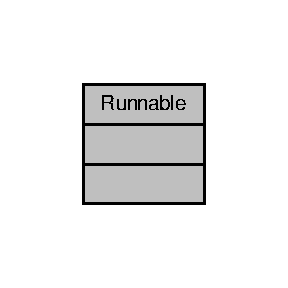
\includegraphics[width=138pt]{class_runnable__coll__graph}
\end{center}
\end{figure}


La documentation de cette classe a été générée à partir du fichier suivant \+:\begin{DoxyCompactItemize}
\item 
\hyperlink{_communication_8java}{Communication.\+java}\end{DoxyCompactItemize}

\hypertarget{classcom_1_1lasalle_1_1meeting_1_1_salle}{}\subsection{Référence de la classe com.\+lasalle.\+meeting.\+Salle}
\label{classcom_1_1lasalle_1_1meeting_1_1_salle}\index{com.\+lasalle.\+meeting.\+Salle@{com.\+lasalle.\+meeting.\+Salle}}


Déclaration de la classe \hyperlink{classcom_1_1lasalle_1_1meeting_1_1_salle}{Salle}.  




Graphe de collaboration de com.\+lasalle.\+meeting.\+Salle\+:
\nopagebreak
\begin{figure}[H]
\begin{center}
\leavevmode
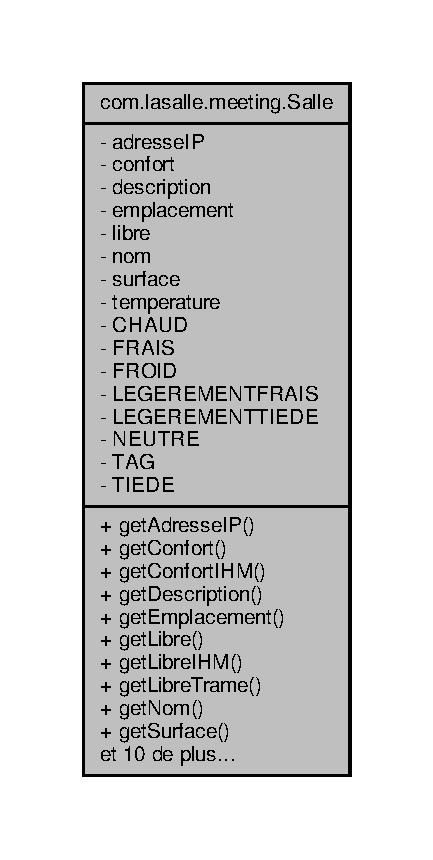
\includegraphics[width=208pt]{classcom_1_1lasalle_1_1meeting_1_1_salle__coll__graph}
\end{center}
\end{figure}
\subsubsection*{Fonctions membres publiques}
\begin{DoxyCompactItemize}
\item 
final String \hyperlink{classcom_1_1lasalle_1_1meeting_1_1_salle_a2189e9d589972421a0f57d045471caa8}{get\+Adresse\+IP} ()
\begin{DoxyCompactList}\small\item\em Accesseur get l\textquotesingle{}adresse IP de la salle. \end{DoxyCompactList}\item 
final int \hyperlink{classcom_1_1lasalle_1_1meeting_1_1_salle_a8f29b7c1302251eed004d0828b7b2ab8}{get\+Confort} ()
\begin{DoxyCompactList}\small\item\em Accesseur get le confort de la salle. \end{DoxyCompactList}\item 
final String \hyperlink{classcom_1_1lasalle_1_1meeting_1_1_salle_abf1f96423a1df46ba4d6ac4a1b6d0c34}{get\+Confort\+I\+HM} ()
\begin{DoxyCompactList}\small\item\em Accesseur get le confort de la salle. \end{DoxyCompactList}\item 
final String \hyperlink{classcom_1_1lasalle_1_1meeting_1_1_salle_a253315cc4da23a4b8ab092e10be6d13d}{get\+Description} ()
\begin{DoxyCompactList}\small\item\em Accesseur get la description de la salle. \end{DoxyCompactList}\item 
final String \hyperlink{classcom_1_1lasalle_1_1meeting_1_1_salle_ac58600d946b6553858cc41be032473cd}{get\+Emplacement} ()
\begin{DoxyCompactList}\small\item\em Accesseur get de l\textquotesingle{}emplacement de la salle. \end{DoxyCompactList}\item 
final boolean \hyperlink{classcom_1_1lasalle_1_1meeting_1_1_salle_adc0c4936355bc0ae22991f69c12a5e42}{get\+Libre} ()
\begin{DoxyCompactList}\small\item\em Accesseur get de libre de la salle. \end{DoxyCompactList}\item 
final String \hyperlink{classcom_1_1lasalle_1_1meeting_1_1_salle_ab86dfb73018e96230ceed49e207a8971}{get\+Libre\+I\+HM} ()
\begin{DoxyCompactList}\small\item\em Accesseur get de libre de la salle. \end{DoxyCompactList}\item 
final String \hyperlink{classcom_1_1lasalle_1_1meeting_1_1_salle_a0039fabf5867aef87f5f61f0081bcbcd}{get\+Libre\+Trame} ()
\begin{DoxyCompactList}\small\item\em Accesseur get de libre de la salle. \end{DoxyCompactList}\item 
final String \hyperlink{classcom_1_1lasalle_1_1meeting_1_1_salle_a49d977f69b2783e8ad57eccffc29e97b}{get\+Nom} ()
\begin{DoxyCompactList}\small\item\em Accesseur get du nom de la salle. \end{DoxyCompactList}\item 
final int \hyperlink{classcom_1_1lasalle_1_1meeting_1_1_salle_ad9dad6b4cfeb020195d4cde268af885f}{get\+Surface} ()
\begin{DoxyCompactList}\small\item\em Accesseur get la surface de la salle. \end{DoxyCompactList}\item 
final float \hyperlink{classcom_1_1lasalle_1_1meeting_1_1_salle_ae3235f548f8bc7ab4d05ff38ec762e77}{get\+Temperature} ()
\begin{DoxyCompactList}\small\item\em Accesseur get la température de la salle. \end{DoxyCompactList}\item 
\hyperlink{classcom_1_1lasalle_1_1meeting_1_1_salle_aa97680026b36fa9e23e8c5c164b8326d}{Salle} (String \hyperlink{classcom_1_1lasalle_1_1meeting_1_1_salle_a3641e82a9fa78c5dc8bd9a5b92bae482}{nom}, String \hyperlink{classcom_1_1lasalle_1_1meeting_1_1_salle_a79547b79b4e812619f6cc764dbe7a80b}{description}, String \hyperlink{classcom_1_1lasalle_1_1meeting_1_1_salle_a9e31fc4d4c9125e511db52da3254bcba}{emplacement}, int \hyperlink{classcom_1_1lasalle_1_1meeting_1_1_salle_a2965cb92b06dcdd28a07fa550259b1c1}{libre}, int \hyperlink{classcom_1_1lasalle_1_1meeting_1_1_salle_a1b761514679fa5f98e71809fea448384}{surface}, int \hyperlink{classcom_1_1lasalle_1_1meeting_1_1_salle_ac165425fc78429c38042a0fed650b9ee}{confort}, float \hyperlink{classcom_1_1lasalle_1_1meeting_1_1_salle_a31600559f77e2eeb1f6aa150b203213e}{temperature}, String \hyperlink{classcom_1_1lasalle_1_1meeting_1_1_salle_ad83f4f49123c8d02f2fc0da484d3e812}{adresse\+IP})
\begin{DoxyCompactList}\small\item\em Constructeur de la classe \hyperlink{classcom_1_1lasalle_1_1meeting_1_1_salle}{Salle}. \end{DoxyCompactList}\item 
void \hyperlink{classcom_1_1lasalle_1_1meeting_1_1_salle_a87125e2e3060bc3d1582dafbdef7b65e}{set\+Adresse\+IP} (String \hyperlink{classcom_1_1lasalle_1_1meeting_1_1_salle_ad83f4f49123c8d02f2fc0da484d3e812}{adresse\+IP})
\begin{DoxyCompactList}\small\item\em Accesseur set l\textquotesingle{}adresse IP de la salle. \end{DoxyCompactList}\item 
void \hyperlink{classcom_1_1lasalle_1_1meeting_1_1_salle_a30986392165b34765e4325f669cc5ece}{set\+Confort} (int nouveau\+Confort)
\begin{DoxyCompactList}\small\item\em Accesseur set du confort de la salle. \end{DoxyCompactList}\item 
void \hyperlink{classcom_1_1lasalle_1_1meeting_1_1_salle_aaa826cdcf54f561daf439c2bf84de5eb}{set\+Emplacement} (String nouvelle\+Emplacement)
\begin{DoxyCompactList}\small\item\em Accesseur set de l\textquotesingle{}emplacement de la salle. \end{DoxyCompactList}\item 
void \hyperlink{classcom_1_1lasalle_1_1meeting_1_1_salle_a94c64624d647ec3ec60a9fbeb06948b8}{set\+Libre} (int \hyperlink{classcom_1_1lasalle_1_1meeting_1_1_salle_a2965cb92b06dcdd28a07fa550259b1c1}{libre})
\begin{DoxyCompactList}\small\item\em Accesseur set la disponibilité de la salle. \end{DoxyCompactList}\item 
void \hyperlink{classcom_1_1lasalle_1_1meeting_1_1_salle_af48c38974e65f48082db016a82afaf89}{set\+Libre} ()
\begin{DoxyCompactList}\small\item\em Accesseur set la disponibilité de la salle, change l\textquotesingle{}état de la salle. \end{DoxyCompactList}\item 
void \hyperlink{classcom_1_1lasalle_1_1meeting_1_1_salle_aad311d55fc41f798532a8a30ea1b68f0}{set\+Nom} (String nouveau\+Nom)
\begin{DoxyCompactList}\small\item\em Accesseur set du nom de la salle. \end{DoxyCompactList}\item 
void \hyperlink{classcom_1_1lasalle_1_1meeting_1_1_salle_ac95af260fcfd0ad267de052cdc0dbeae}{set\+Surface} (int nouvelle\+Surface)
\begin{DoxyCompactList}\small\item\em Accesseur set la surface de la salle. \end{DoxyCompactList}\item 
void \hyperlink{classcom_1_1lasalle_1_1meeting_1_1_salle_ae618bd9da7fd68e4789b3d87a4aa90b3}{set\+Temperature} (float \hyperlink{classcom_1_1lasalle_1_1meeting_1_1_salle_a31600559f77e2eeb1f6aa150b203213e}{temperature})
\begin{DoxyCompactList}\small\item\em Accesseur set la température de la salle. \end{DoxyCompactList}\end{DoxyCompactItemize}
\subsubsection*{Attributs privés}
\begin{DoxyCompactItemize}
\item 
String \hyperlink{classcom_1_1lasalle_1_1meeting_1_1_salle_ad83f4f49123c8d02f2fc0da484d3e812}{adresse\+IP}
\begin{DoxyCompactList}\small\item\em l\textquotesingle{}adresse IP de la salle \end{DoxyCompactList}\item 
int \hyperlink{classcom_1_1lasalle_1_1meeting_1_1_salle_ac165425fc78429c38042a0fed650b9ee}{confort}
\begin{DoxyCompactList}\small\item\em le niveau de confort de la salle \end{DoxyCompactList}\item 
String \hyperlink{classcom_1_1lasalle_1_1meeting_1_1_salle_a79547b79b4e812619f6cc764dbe7a80b}{description} = \char`\"{}\char`\"{}
\begin{DoxyCompactList}\small\item\em La description de la salle. \end{DoxyCompactList}\item 
String \hyperlink{classcom_1_1lasalle_1_1meeting_1_1_salle_a9e31fc4d4c9125e511db52da3254bcba}{emplacement} = \char`\"{}\char`\"{}
\begin{DoxyCompactList}\small\item\em L\textquotesingle{}emplacement de la salle. \end{DoxyCompactList}\item 
boolean \hyperlink{classcom_1_1lasalle_1_1meeting_1_1_salle_a2965cb92b06dcdd28a07fa550259b1c1}{libre}
\begin{DoxyCompactList}\small\item\em L\textquotesingle{}état booléen d\textquotesingle{}occupation Libre de la salle. \end{DoxyCompactList}\item 
String \hyperlink{classcom_1_1lasalle_1_1meeting_1_1_salle_a3641e82a9fa78c5dc8bd9a5b92bae482}{nom} = \char`\"{}\char`\"{}
\begin{DoxyCompactList}\small\item\em Le nom de la salle. \end{DoxyCompactList}\item 
int \hyperlink{classcom_1_1lasalle_1_1meeting_1_1_salle_a1b761514679fa5f98e71809fea448384}{surface}
\begin{DoxyCompactList}\small\item\em la surface de la salle \end{DoxyCompactList}\item 
float \hyperlink{classcom_1_1lasalle_1_1meeting_1_1_salle_a31600559f77e2eeb1f6aa150b203213e}{temperature}
\begin{DoxyCompactList}\small\item\em la température de la salle \end{DoxyCompactList}\end{DoxyCompactItemize}
\subsubsection*{Attributs privés statiques}
\begin{DoxyCompactItemize}
\item 
static final int \hyperlink{classcom_1_1lasalle_1_1meeting_1_1_salle_af9e1ab39b745ab56a29910452fcc9814}{C\+H\+A\+UD} = 3
\begin{DoxyCompactList}\small\item\em Constant niveau de confort C\+H\+A\+UD. \end{DoxyCompactList}\item 
static final int \hyperlink{classcom_1_1lasalle_1_1meeting_1_1_salle_aff34072175ff3c1bc425a8bacc31ff4b}{F\+R\+A\+IS} = -\/2
\begin{DoxyCompactList}\small\item\em Constant niveau de confort F\+R\+A\+IS. \end{DoxyCompactList}\item 
static final int \hyperlink{classcom_1_1lasalle_1_1meeting_1_1_salle_a1b29ac9518653cc15391c4deed380fbb}{F\+R\+O\+ID} = -\/3
\begin{DoxyCompactList}\small\item\em Constant niveau de confort F\+R\+O\+ID. \end{DoxyCompactList}\item 
static final int \hyperlink{classcom_1_1lasalle_1_1meeting_1_1_salle_a5a7a447ea3cef14da14b9137c0491015}{L\+E\+G\+E\+R\+E\+M\+E\+N\+T\+F\+R\+A\+IS} = -\/1
\begin{DoxyCompactList}\small\item\em Constant niveau de confort L\+E\+G\+E\+R\+E\+M\+E\+N\+T\+F\+R\+A\+IS. \end{DoxyCompactList}\item 
static final int \hyperlink{classcom_1_1lasalle_1_1meeting_1_1_salle_ab12c81e0c36cf771febef1a160a1998b}{L\+E\+G\+E\+R\+E\+M\+E\+N\+T\+T\+I\+E\+DE} = 1
\begin{DoxyCompactList}\small\item\em Constant niveau de confort L\+E\+G\+E\+R\+E\+M\+E\+N\+T\+T\+I\+E\+DE. \end{DoxyCompactList}\item 
static final int \hyperlink{classcom_1_1lasalle_1_1meeting_1_1_salle_aeffa1f0543757746e8376ff8495fcedd}{N\+E\+U\+T\+RE} = 0
\begin{DoxyCompactList}\small\item\em Constant niveau de confort N\+E\+U\+T\+RE. \end{DoxyCompactList}\item 
static final String \hyperlink{classcom_1_1lasalle_1_1meeting_1_1_salle_aecf7e402dafb939f8ac2f2873f66af25}{T\+AG} = \char`\"{}Salle\char`\"{}
\begin{DoxyCompactList}\small\item\em T\+AG utilisé pour les logs. \end{DoxyCompactList}\item 
static final int \hyperlink{classcom_1_1lasalle_1_1meeting_1_1_salle_ab6fdb3566901998a91c1cd17f589f607}{T\+I\+E\+DE} = 2
\begin{DoxyCompactList}\small\item\em Constant niveau de confort T\+I\+E\+DE. \end{DoxyCompactList}\end{DoxyCompactItemize}


\subsubsection{Description détaillée}
Déclaration de la classe \hyperlink{classcom_1_1lasalle_1_1meeting_1_1_salle}{Salle}. 

Définition à la ligne \hyperlink{_salle_8java_source_l00017}{17} du fichier \hyperlink{_salle_8java_source}{Salle.\+java}.



\subsubsection{Documentation des constructeurs et destructeur}
\mbox{\Hypertarget{classcom_1_1lasalle_1_1meeting_1_1_salle_aa97680026b36fa9e23e8c5c164b8326d}\label{classcom_1_1lasalle_1_1meeting_1_1_salle_aa97680026b36fa9e23e8c5c164b8326d}} 
\index{com\+::lasalle\+::meeting\+::\+Salle@{com\+::lasalle\+::meeting\+::\+Salle}!Salle@{Salle}}
\index{Salle@{Salle}!com\+::lasalle\+::meeting\+::\+Salle@{com\+::lasalle\+::meeting\+::\+Salle}}
\paragraph{\texorpdfstring{Salle()}{Salle()}}
{\footnotesize\ttfamily com.\+lasalle.\+meeting.\+Salle.\+Salle (\begin{DoxyParamCaption}\item[{String}]{nom,  }\item[{String}]{description,  }\item[{String}]{emplacement,  }\item[{int}]{libre,  }\item[{int}]{surface,  }\item[{int}]{confort,  }\item[{float}]{temperature,  }\item[{String}]{adresse\+IP }\end{DoxyParamCaption})}



Constructeur de la classe \hyperlink{classcom_1_1lasalle_1_1meeting_1_1_salle}{Salle}. 


\begin{DoxyParams}{Paramètres}
{\em nom} & \\
\hline
{\em description} & \\
\hline
{\em emplacement} & \\
\hline
{\em libre} & \\
\hline
{\em surface} & \\
\hline
{\em temperature} & \\
\hline
{\em adresse\+IP} & \\
\hline
\end{DoxyParams}


Définition à la ligne \hyperlink{_salle_8java_source_l00054}{54} du fichier \hyperlink{_salle_8java_source}{Salle.\+java}.



Références \hyperlink{_salle_8java_source_l00041}{com.\+lasalle.\+meeting.\+Salle.\+adresse\+IP}, \hyperlink{_salle_8java_source_l00039}{com.\+lasalle.\+meeting.\+Salle.\+confort}, \hyperlink{_salle_8java_source_l00035}{com.\+lasalle.\+meeting.\+Salle.\+description}, \hyperlink{_salle_8java_source_l00036}{com.\+lasalle.\+meeting.\+Salle.\+emplacement}, \hyperlink{_salle_8java_source_l00034}{com.\+lasalle.\+meeting.\+Salle.\+nom}, \hyperlink{_salle_8java_source_l00104}{com.\+lasalle.\+meeting.\+Salle.\+set\+Libre()}, \hyperlink{_salle_8java_source_l00038}{com.\+lasalle.\+meeting.\+Salle.\+surface}, et \hyperlink{_salle_8java_source_l00040}{com.\+lasalle.\+meeting.\+Salle.\+temperature}.


\begin{DoxyCode}
00055     \{
00056         this.\hyperlink{classcom_1_1lasalle_1_1meeting_1_1_salle_a3641e82a9fa78c5dc8bd9a5b92bae482}{nom} = \hyperlink{classcom_1_1lasalle_1_1meeting_1_1_salle_a3641e82a9fa78c5dc8bd9a5b92bae482}{nom};
00057         this.\hyperlink{classcom_1_1lasalle_1_1meeting_1_1_salle_a79547b79b4e812619f6cc764dbe7a80b}{description} = \hyperlink{classcom_1_1lasalle_1_1meeting_1_1_salle_a79547b79b4e812619f6cc764dbe7a80b}{description};
00058         this.\hyperlink{classcom_1_1lasalle_1_1meeting_1_1_salle_a9e31fc4d4c9125e511db52da3254bcba}{emplacement} = \hyperlink{classcom_1_1lasalle_1_1meeting_1_1_salle_a9e31fc4d4c9125e511db52da3254bcba}{emplacement};
00059         \hyperlink{classcom_1_1lasalle_1_1meeting_1_1_salle_af48c38974e65f48082db016a82afaf89}{setLibre}(\hyperlink{classcom_1_1lasalle_1_1meeting_1_1_salle_a2965cb92b06dcdd28a07fa550259b1c1}{libre});
00060         this.\hyperlink{classcom_1_1lasalle_1_1meeting_1_1_salle_a1b761514679fa5f98e71809fea448384}{surface} = \hyperlink{classcom_1_1lasalle_1_1meeting_1_1_salle_a1b761514679fa5f98e71809fea448384}{surface};
00061         this.\hyperlink{classcom_1_1lasalle_1_1meeting_1_1_salle_ac165425fc78429c38042a0fed650b9ee}{confort} = \hyperlink{classcom_1_1lasalle_1_1meeting_1_1_salle_ac165425fc78429c38042a0fed650b9ee}{confort};
00062         this.\hyperlink{classcom_1_1lasalle_1_1meeting_1_1_salle_a31600559f77e2eeb1f6aa150b203213e}{temperature} = \hyperlink{classcom_1_1lasalle_1_1meeting_1_1_salle_a31600559f77e2eeb1f6aa150b203213e}{temperature};
00063         this.\hyperlink{classcom_1_1lasalle_1_1meeting_1_1_salle_ad83f4f49123c8d02f2fc0da484d3e812}{adresseIP} = \hyperlink{classcom_1_1lasalle_1_1meeting_1_1_salle_ad83f4f49123c8d02f2fc0da484d3e812}{adresseIP};
00064         Log.d(\hyperlink{classcom_1_1lasalle_1_1meeting_1_1_salle_aecf7e402dafb939f8ac2f2873f66af25}{TAG}, \textcolor{stringliteral}{"Salle : nom = "} + \hyperlink{classcom_1_1lasalle_1_1meeting_1_1_salle_a3641e82a9fa78c5dc8bd9a5b92bae482}{nom} + \textcolor{stringliteral}{" - description = "} + 
      \hyperlink{classcom_1_1lasalle_1_1meeting_1_1_salle_a79547b79b4e812619f6cc764dbe7a80b}{description} + \textcolor{stringliteral}{" - emplacement "} + \hyperlink{classcom_1_1lasalle_1_1meeting_1_1_salle_a9e31fc4d4c9125e511db52da3254bcba}{emplacement} + \textcolor{stringliteral}{" - libre = "} + 
      \hyperlink{classcom_1_1lasalle_1_1meeting_1_1_salle_a2965cb92b06dcdd28a07fa550259b1c1}{libre} + \textcolor{stringliteral}{" - surface = "} + \hyperlink{classcom_1_1lasalle_1_1meeting_1_1_salle_a1b761514679fa5f98e71809fea448384}{surface} + \textcolor{stringliteral}{" - confort = "} + \hyperlink{classcom_1_1lasalle_1_1meeting_1_1_salle_ac165425fc78429c38042a0fed650b9ee}{confort} + \textcolor{stringliteral}{" - température = "} + 
      \hyperlink{classcom_1_1lasalle_1_1meeting_1_1_salle_a31600559f77e2eeb1f6aa150b203213e}{temperature} + \textcolor{stringliteral}{" - adresseIP = "} + \hyperlink{classcom_1_1lasalle_1_1meeting_1_1_salle_ad83f4f49123c8d02f2fc0da484d3e812}{adresseIP});
00065     \}
\end{DoxyCode}


\subsubsection{Documentation des fonctions membres}
\mbox{\Hypertarget{classcom_1_1lasalle_1_1meeting_1_1_salle_a2189e9d589972421a0f57d045471caa8}\label{classcom_1_1lasalle_1_1meeting_1_1_salle_a2189e9d589972421a0f57d045471caa8}} 
\index{com\+::lasalle\+::meeting\+::\+Salle@{com\+::lasalle\+::meeting\+::\+Salle}!get\+Adresse\+IP@{get\+Adresse\+IP}}
\index{get\+Adresse\+IP@{get\+Adresse\+IP}!com\+::lasalle\+::meeting\+::\+Salle@{com\+::lasalle\+::meeting\+::\+Salle}}
\paragraph{\texorpdfstring{get\+Adresse\+I\+P()}{getAdresseIP()}}
{\footnotesize\ttfamily final String com.\+lasalle.\+meeting.\+Salle.\+get\+Adresse\+IP (\begin{DoxyParamCaption}{ }\end{DoxyParamCaption})}



Accesseur get l\textquotesingle{}adresse IP de la salle. 

\begin{DoxyReturn}{Renvoie}
String l\textquotesingle{}adresse IP de la salle 
\end{DoxyReturn}


Définition à la ligne \hyperlink{_salle_8java_source_l00285}{285} du fichier \hyperlink{_salle_8java_source}{Salle.\+java}.



Références \hyperlink{_salle_8java_source_l00041}{com.\+lasalle.\+meeting.\+Salle.\+adresse\+IP}.



Référencé par \hyperlink{_salle_activity_8java_source_l00132}{com.\+lasalle.\+meeting.\+Salle\+Activity.\+set\+Listener()}, et \hyperlink{_main_activity_8java_source_l00261}{com.\+lasalle.\+meeting.\+Main\+Activity.\+verifier\+Existence\+Salle()}.


\begin{DoxyCode}
00286     \{
00287         \textcolor{keywordflow}{return} \hyperlink{classcom_1_1lasalle_1_1meeting_1_1_salle_ad83f4f49123c8d02f2fc0da484d3e812}{adresseIP};
00288     \}
\end{DoxyCode}
\mbox{\Hypertarget{classcom_1_1lasalle_1_1meeting_1_1_salle_a8f29b7c1302251eed004d0828b7b2ab8}\label{classcom_1_1lasalle_1_1meeting_1_1_salle_a8f29b7c1302251eed004d0828b7b2ab8}} 
\index{com\+::lasalle\+::meeting\+::\+Salle@{com\+::lasalle\+::meeting\+::\+Salle}!get\+Confort@{get\+Confort}}
\index{get\+Confort@{get\+Confort}!com\+::lasalle\+::meeting\+::\+Salle@{com\+::lasalle\+::meeting\+::\+Salle}}
\paragraph{\texorpdfstring{get\+Confort()}{getConfort()}}
{\footnotesize\ttfamily final int com.\+lasalle.\+meeting.\+Salle.\+get\+Confort (\begin{DoxyParamCaption}{ }\end{DoxyParamCaption})}



Accesseur get le confort de la salle. 

\begin{DoxyReturn}{Renvoie}
int le niveau de confort de la salle 
\end{DoxyReturn}


Définition à la ligne \hyperlink{_salle_8java_source_l00224}{224} du fichier \hyperlink{_salle_8java_source}{Salle.\+java}.



Références \hyperlink{_salle_8java_source_l00039}{com.\+lasalle.\+meeting.\+Salle.\+confort}.



Référencé par \hyperlink{_main_activity_8java_source_l00291}{com.\+lasalle.\+meeting.\+Main\+Activity.\+verifier\+Changement\+Salle()}.


\begin{DoxyCode}
00225     \{
00226         \textcolor{keywordflow}{return} \hyperlink{classcom_1_1lasalle_1_1meeting_1_1_salle_ac165425fc78429c38042a0fed650b9ee}{confort};
00227     \}
\end{DoxyCode}
\mbox{\Hypertarget{classcom_1_1lasalle_1_1meeting_1_1_salle_abf1f96423a1df46ba4d6ac4a1b6d0c34}\label{classcom_1_1lasalle_1_1meeting_1_1_salle_abf1f96423a1df46ba4d6ac4a1b6d0c34}} 
\index{com\+::lasalle\+::meeting\+::\+Salle@{com\+::lasalle\+::meeting\+::\+Salle}!get\+Confort\+I\+HM@{get\+Confort\+I\+HM}}
\index{get\+Confort\+I\+HM@{get\+Confort\+I\+HM}!com\+::lasalle\+::meeting\+::\+Salle@{com\+::lasalle\+::meeting\+::\+Salle}}
\paragraph{\texorpdfstring{get\+Confort\+I\+H\+M()}{getConfortIHM()}}
{\footnotesize\ttfamily final String com.\+lasalle.\+meeting.\+Salle.\+get\+Confort\+I\+HM (\begin{DoxyParamCaption}{ }\end{DoxyParamCaption})}



Accesseur get le confort de la salle. 

\begin{DoxyReturn}{Renvoie}
String le niveau de confort de la salle, pour l\textquotesingle{}affichage 
\end{DoxyReturn}


Définition à la ligne \hyperlink{_salle_8java_source_l00233}{233} du fichier \hyperlink{_salle_8java_source}{Salle.\+java}.



Références \hyperlink{_salle_8java_source_l00029}{com.\+lasalle.\+meeting.\+Salle.\+C\+H\+A\+UD}, \hyperlink{_salle_8java_source_l00024}{com.\+lasalle.\+meeting.\+Salle.\+F\+R\+A\+IS}, \hyperlink{_salle_8java_source_l00023}{com.\+lasalle.\+meeting.\+Salle.\+F\+R\+O\+ID}, \hyperlink{_salle_8java_source_l00025}{com.\+lasalle.\+meeting.\+Salle.\+L\+E\+G\+E\+R\+E\+M\+E\+N\+T\+F\+R\+A\+IS}, \hyperlink{_salle_8java_source_l00027}{com.\+lasalle.\+meeting.\+Salle.\+L\+E\+G\+E\+R\+E\+M\+E\+N\+T\+T\+I\+E\+DE}, \hyperlink{_salle_8java_source_l00026}{com.\+lasalle.\+meeting.\+Salle.\+N\+E\+U\+T\+RE}, et \hyperlink{_salle_8java_source_l00028}{com.\+lasalle.\+meeting.\+Salle.\+T\+I\+E\+DE}.



Référencé par \hyperlink{_salle_view_holder_8java_source_l00077}{com.\+lasalle.\+meeting.\+Salle\+View\+Holder.\+afficher()}, et \hyperlink{_salle_activity_8java_source_l00103}{com.\+lasalle.\+meeting.\+Salle\+Activity.\+afficher\+Information\+Salle()}.


\begin{DoxyCode}
00234     \{
00235         String message = \textcolor{stringliteral}{""};
00236         \textcolor{keywordflow}{switch} (\hyperlink{classcom_1_1lasalle_1_1meeting_1_1_salle_ac165425fc78429c38042a0fed650b9ee}{confort})
00237         \{
00238             \textcolor{keywordflow}{case} \hyperlink{classcom_1_1lasalle_1_1meeting_1_1_salle_a1b29ac9518653cc15391c4deed380fbb}{FROID}:
00239                 message = \textcolor{stringliteral}{"Confort : Froid"};
00240                 \textcolor{keywordflow}{break};
00241             \textcolor{keywordflow}{case} \hyperlink{classcom_1_1lasalle_1_1meeting_1_1_salle_aff34072175ff3c1bc425a8bacc31ff4b}{FRAIS}:
00242                 message = \textcolor{stringliteral}{"Confort : Frais"};
00243                 \textcolor{keywordflow}{break};
00244             \textcolor{keywordflow}{case} \hyperlink{classcom_1_1lasalle_1_1meeting_1_1_salle_a5a7a447ea3cef14da14b9137c0491015}{LEGEREMENTFRAIS}:
00245                 message = \textcolor{stringliteral}{"Confort : Légèrement frais"};
00246                 \textcolor{keywordflow}{break};
00247             \textcolor{keywordflow}{case} \hyperlink{classcom_1_1lasalle_1_1meeting_1_1_salle_aeffa1f0543757746e8376ff8495fcedd}{NEUTRE}:
00248                 message = \textcolor{stringliteral}{"Confort : Neutre"};
00249                 \textcolor{keywordflow}{break};
00250             \textcolor{keywordflow}{case} \hyperlink{classcom_1_1lasalle_1_1meeting_1_1_salle_ab12c81e0c36cf771febef1a160a1998b}{LEGEREMENTTIEDE}:
00251                 message = \textcolor{stringliteral}{"Confort : Légèrement tiède"};
00252                 \textcolor{keywordflow}{break};
00253             \textcolor{keywordflow}{case} \hyperlink{classcom_1_1lasalle_1_1meeting_1_1_salle_ab6fdb3566901998a91c1cd17f589f607}{TIEDE}:
00254                 message = \textcolor{stringliteral}{"Confort : Tiède"};
00255                 \textcolor{keywordflow}{break};
00256             \textcolor{keywordflow}{case} \hyperlink{classcom_1_1lasalle_1_1meeting_1_1_salle_af9e1ab39b745ab56a29910452fcc9814}{CHAUD}:
00257                 message = \textcolor{stringliteral}{"Confort : Chaud"};
00258                 \textcolor{keywordflow}{break};
00259         \}
00260         \textcolor{keywordflow}{return} message;
00261     \}
\end{DoxyCode}
\mbox{\Hypertarget{classcom_1_1lasalle_1_1meeting_1_1_salle_a253315cc4da23a4b8ab092e10be6d13d}\label{classcom_1_1lasalle_1_1meeting_1_1_salle_a253315cc4da23a4b8ab092e10be6d13d}} 
\index{com\+::lasalle\+::meeting\+::\+Salle@{com\+::lasalle\+::meeting\+::\+Salle}!get\+Description@{get\+Description}}
\index{get\+Description@{get\+Description}!com\+::lasalle\+::meeting\+::\+Salle@{com\+::lasalle\+::meeting\+::\+Salle}}
\paragraph{\texorpdfstring{get\+Description()}{getDescription()}}
{\footnotesize\ttfamily final String com.\+lasalle.\+meeting.\+Salle.\+get\+Description (\begin{DoxyParamCaption}{ }\end{DoxyParamCaption})}



Accesseur get la description de la salle. 

\begin{DoxyReturn}{Renvoie}
String la description de la salle 
\end{DoxyReturn}


Définition à la ligne \hyperlink{_salle_8java_source_l00276}{276} du fichier \hyperlink{_salle_8java_source}{Salle.\+java}.



Références \hyperlink{_salle_8java_source_l00035}{com.\+lasalle.\+meeting.\+Salle.\+description}.



Référencé par \hyperlink{_salle_activity_8java_source_l00103}{com.\+lasalle.\+meeting.\+Salle\+Activity.\+afficher\+Information\+Salle()}, et \hyperlink{_main_activity_8java_source_l00291}{com.\+lasalle.\+meeting.\+Main\+Activity.\+verifier\+Changement\+Salle()}.


\begin{DoxyCode}
00277     \{
00278         \textcolor{keywordflow}{return} \hyperlink{classcom_1_1lasalle_1_1meeting_1_1_salle_a79547b79b4e812619f6cc764dbe7a80b}{description};
00279     \}
\end{DoxyCode}
\mbox{\Hypertarget{classcom_1_1lasalle_1_1meeting_1_1_salle_ac58600d946b6553858cc41be032473cd}\label{classcom_1_1lasalle_1_1meeting_1_1_salle_ac58600d946b6553858cc41be032473cd}} 
\index{com\+::lasalle\+::meeting\+::\+Salle@{com\+::lasalle\+::meeting\+::\+Salle}!get\+Emplacement@{get\+Emplacement}}
\index{get\+Emplacement@{get\+Emplacement}!com\+::lasalle\+::meeting\+::\+Salle@{com\+::lasalle\+::meeting\+::\+Salle}}
\paragraph{\texorpdfstring{get\+Emplacement()}{getEmplacement()}}
{\footnotesize\ttfamily final String com.\+lasalle.\+meeting.\+Salle.\+get\+Emplacement (\begin{DoxyParamCaption}{ }\end{DoxyParamCaption})}



Accesseur get de l\textquotesingle{}emplacement de la salle. 

\begin{DoxyReturn}{Renvoie}
String l\textquotesingle{}emplacement de la salle 
\end{DoxyReturn}


Définition à la ligne \hyperlink{_salle_8java_source_l00156}{156} du fichier \hyperlink{_salle_8java_source}{Salle.\+java}.



Références \hyperlink{_salle_8java_source_l00036}{com.\+lasalle.\+meeting.\+Salle.\+emplacement}.



Référencé par \hyperlink{_salle_activity_8java_source_l00103}{com.\+lasalle.\+meeting.\+Salle\+Activity.\+afficher\+Information\+Salle()}, et \hyperlink{_main_activity_8java_source_l00291}{com.\+lasalle.\+meeting.\+Main\+Activity.\+verifier\+Changement\+Salle()}.


\begin{DoxyCode}
00157     \{
00158         \textcolor{keywordflow}{return} \hyperlink{classcom_1_1lasalle_1_1meeting_1_1_salle_a9e31fc4d4c9125e511db52da3254bcba}{emplacement};
00159     \}
\end{DoxyCode}
\mbox{\Hypertarget{classcom_1_1lasalle_1_1meeting_1_1_salle_adc0c4936355bc0ae22991f69c12a5e42}\label{classcom_1_1lasalle_1_1meeting_1_1_salle_adc0c4936355bc0ae22991f69c12a5e42}} 
\index{com\+::lasalle\+::meeting\+::\+Salle@{com\+::lasalle\+::meeting\+::\+Salle}!get\+Libre@{get\+Libre}}
\index{get\+Libre@{get\+Libre}!com\+::lasalle\+::meeting\+::\+Salle@{com\+::lasalle\+::meeting\+::\+Salle}}
\paragraph{\texorpdfstring{get\+Libre()}{getLibre()}}
{\footnotesize\ttfamily final boolean com.\+lasalle.\+meeting.\+Salle.\+get\+Libre (\begin{DoxyParamCaption}{ }\end{DoxyParamCaption})}



Accesseur get de libre de la salle. 

\begin{DoxyReturn}{Renvoie}
boolean la disponibilité de la salle 
\end{DoxyReturn}


Définition à la ligne \hyperlink{_salle_8java_source_l00174}{174} du fichier \hyperlink{_salle_8java_source}{Salle.\+java}.



Références \hyperlink{_salle_8java_source_l00037}{com.\+lasalle.\+meeting.\+Salle.\+libre}.



Référencé par \hyperlink{_salle_view_holder_8java_source_l00077}{com.\+lasalle.\+meeting.\+Salle\+View\+Holder.\+afficher()}, \hyperlink{_salle_activity_8java_source_l00103}{com.\+lasalle.\+meeting.\+Salle\+Activity.\+afficher\+Information\+Salle()}, \hyperlink{_salle_activity_8java_source_l00085}{com.\+lasalle.\+meeting.\+Salle\+Activity.\+set\+Bouton\+Change\+Etat()}, et \hyperlink{_main_activity_8java_source_l00291}{com.\+lasalle.\+meeting.\+Main\+Activity.\+verifier\+Changement\+Salle()}.


\begin{DoxyCode}
00175     \{
00176         \textcolor{keywordflow}{return} \hyperlink{classcom_1_1lasalle_1_1meeting_1_1_salle_a2965cb92b06dcdd28a07fa550259b1c1}{libre};
00177     \}
\end{DoxyCode}
\mbox{\Hypertarget{classcom_1_1lasalle_1_1meeting_1_1_salle_ab86dfb73018e96230ceed49e207a8971}\label{classcom_1_1lasalle_1_1meeting_1_1_salle_ab86dfb73018e96230ceed49e207a8971}} 
\index{com\+::lasalle\+::meeting\+::\+Salle@{com\+::lasalle\+::meeting\+::\+Salle}!get\+Libre\+I\+HM@{get\+Libre\+I\+HM}}
\index{get\+Libre\+I\+HM@{get\+Libre\+I\+HM}!com\+::lasalle\+::meeting\+::\+Salle@{com\+::lasalle\+::meeting\+::\+Salle}}
\paragraph{\texorpdfstring{get\+Libre\+I\+H\+M()}{getLibreIHM()}}
{\footnotesize\ttfamily final String com.\+lasalle.\+meeting.\+Salle.\+get\+Libre\+I\+HM (\begin{DoxyParamCaption}{ }\end{DoxyParamCaption})}



Accesseur get de libre de la salle. 

\begin{DoxyReturn}{Renvoie}
String la disponibilité de la salle, pour l\textquotesingle{}affichage 
\end{DoxyReturn}


Définition à la ligne \hyperlink{_salle_8java_source_l00199}{199} du fichier \hyperlink{_salle_8java_source}{Salle.\+java}.



Référencé par \hyperlink{_salle_view_holder_8java_source_l00077}{com.\+lasalle.\+meeting.\+Salle\+View\+Holder.\+afficher()}.


\begin{DoxyCode}
00200     \{
00201         \textcolor{keywordflow}{if}(\hyperlink{classcom_1_1lasalle_1_1meeting_1_1_salle_a2965cb92b06dcdd28a07fa550259b1c1}{libre} == \textcolor{keyword}{false})
00202         \{
00203             \textcolor{keywordflow}{return} \textcolor{stringliteral}{"occupée"};
00204         \}
00205         \textcolor{keywordflow}{else}
00206         \{
00207             \textcolor{keywordflow}{return} \textcolor{stringliteral}{"disponible"};
00208         \}
00209     \}
\end{DoxyCode}
\mbox{\Hypertarget{classcom_1_1lasalle_1_1meeting_1_1_salle_a0039fabf5867aef87f5f61f0081bcbcd}\label{classcom_1_1lasalle_1_1meeting_1_1_salle_a0039fabf5867aef87f5f61f0081bcbcd}} 
\index{com\+::lasalle\+::meeting\+::\+Salle@{com\+::lasalle\+::meeting\+::\+Salle}!get\+Libre\+Trame@{get\+Libre\+Trame}}
\index{get\+Libre\+Trame@{get\+Libre\+Trame}!com\+::lasalle\+::meeting\+::\+Salle@{com\+::lasalle\+::meeting\+::\+Salle}}
\paragraph{\texorpdfstring{get\+Libre\+Trame()}{getLibreTrame()}}
{\footnotesize\ttfamily final String com.\+lasalle.\+meeting.\+Salle.\+get\+Libre\+Trame (\begin{DoxyParamCaption}{ }\end{DoxyParamCaption})}



Accesseur get de libre de la salle. 

\begin{DoxyReturn}{Renvoie}
String la disponibilité de la salle, pour la trame 
\end{DoxyReturn}


Définition à la ligne \hyperlink{_salle_8java_source_l00183}{183} du fichier \hyperlink{_salle_8java_source}{Salle.\+java}.



Référencé par \hyperlink{_salle_activity_8java_source_l00132}{com.\+lasalle.\+meeting.\+Salle\+Activity.\+set\+Listener()}.


\begin{DoxyCode}
00184     \{
00185         \textcolor{keywordflow}{if}(\hyperlink{classcom_1_1lasalle_1_1meeting_1_1_salle_a2965cb92b06dcdd28a07fa550259b1c1}{libre} == \textcolor{keyword}{false})
00186         \{
00187             \textcolor{keywordflow}{return} \textcolor{stringliteral}{"0"};
00188         \}
00189         \textcolor{keywordflow}{else}
00190         \{
00191             \textcolor{keywordflow}{return} \textcolor{stringliteral}{"1"};
00192         \}
00193     \}
\end{DoxyCode}
\mbox{\Hypertarget{classcom_1_1lasalle_1_1meeting_1_1_salle_a49d977f69b2783e8ad57eccffc29e97b}\label{classcom_1_1lasalle_1_1meeting_1_1_salle_a49d977f69b2783e8ad57eccffc29e97b}} 
\index{com\+::lasalle\+::meeting\+::\+Salle@{com\+::lasalle\+::meeting\+::\+Salle}!get\+Nom@{get\+Nom}}
\index{get\+Nom@{get\+Nom}!com\+::lasalle\+::meeting\+::\+Salle@{com\+::lasalle\+::meeting\+::\+Salle}}
\paragraph{\texorpdfstring{get\+Nom()}{getNom()}}
{\footnotesize\ttfamily final String com.\+lasalle.\+meeting.\+Salle.\+get\+Nom (\begin{DoxyParamCaption}{ }\end{DoxyParamCaption})}



Accesseur get du nom de la salle. 

\begin{DoxyReturn}{Renvoie}
String le nom de la salle 
\end{DoxyReturn}


Définition à la ligne \hyperlink{_salle_8java_source_l00165}{165} du fichier \hyperlink{_salle_8java_source}{Salle.\+java}.



Références \hyperlink{_salle_8java_source_l00034}{com.\+lasalle.\+meeting.\+Salle.\+nom}.



Référencé par \hyperlink{_salle_view_holder_8java_source_l00077}{com.\+lasalle.\+meeting.\+Salle\+View\+Holder.\+afficher()}, \hyperlink{_salle_activity_8java_source_l00103}{com.\+lasalle.\+meeting.\+Salle\+Activity.\+afficher\+Information\+Salle()}, \hyperlink{_salle_activity_8java_source_l00060}{com.\+lasalle.\+meeting.\+Salle\+Activity.\+on\+Create()}, et \hyperlink{_main_activity_8java_source_l00291}{com.\+lasalle.\+meeting.\+Main\+Activity.\+verifier\+Changement\+Salle()}.


\begin{DoxyCode}
00166     \{
00167         \textcolor{keywordflow}{return} \hyperlink{classcom_1_1lasalle_1_1meeting_1_1_salle_a3641e82a9fa78c5dc8bd9a5b92bae482}{nom};
00168     \}
\end{DoxyCode}
\mbox{\Hypertarget{classcom_1_1lasalle_1_1meeting_1_1_salle_ad9dad6b4cfeb020195d4cde268af885f}\label{classcom_1_1lasalle_1_1meeting_1_1_salle_ad9dad6b4cfeb020195d4cde268af885f}} 
\index{com\+::lasalle\+::meeting\+::\+Salle@{com\+::lasalle\+::meeting\+::\+Salle}!get\+Surface@{get\+Surface}}
\index{get\+Surface@{get\+Surface}!com\+::lasalle\+::meeting\+::\+Salle@{com\+::lasalle\+::meeting\+::\+Salle}}
\paragraph{\texorpdfstring{get\+Surface()}{getSurface()}}
{\footnotesize\ttfamily final int com.\+lasalle.\+meeting.\+Salle.\+get\+Surface (\begin{DoxyParamCaption}{ }\end{DoxyParamCaption})}



Accesseur get la surface de la salle. 

\begin{DoxyReturn}{Renvoie}
int la surface de la salle 
\end{DoxyReturn}


Définition à la ligne \hyperlink{_salle_8java_source_l00215}{215} du fichier \hyperlink{_salle_8java_source}{Salle.\+java}.



Références \hyperlink{_salle_8java_source_l00038}{com.\+lasalle.\+meeting.\+Salle.\+surface}.



Référencé par \hyperlink{_salle_activity_8java_source_l00103}{com.\+lasalle.\+meeting.\+Salle\+Activity.\+afficher\+Information\+Salle()}, et \hyperlink{_main_activity_8java_source_l00291}{com.\+lasalle.\+meeting.\+Main\+Activity.\+verifier\+Changement\+Salle()}.


\begin{DoxyCode}
00216     \{
00217         \textcolor{keywordflow}{return} \hyperlink{classcom_1_1lasalle_1_1meeting_1_1_salle_a1b761514679fa5f98e71809fea448384}{surface};
00218     \}
\end{DoxyCode}
\mbox{\Hypertarget{classcom_1_1lasalle_1_1meeting_1_1_salle_ae3235f548f8bc7ab4d05ff38ec762e77}\label{classcom_1_1lasalle_1_1meeting_1_1_salle_ae3235f548f8bc7ab4d05ff38ec762e77}} 
\index{com\+::lasalle\+::meeting\+::\+Salle@{com\+::lasalle\+::meeting\+::\+Salle}!get\+Temperature@{get\+Temperature}}
\index{get\+Temperature@{get\+Temperature}!com\+::lasalle\+::meeting\+::\+Salle@{com\+::lasalle\+::meeting\+::\+Salle}}
\paragraph{\texorpdfstring{get\+Temperature()}{getTemperature()}}
{\footnotesize\ttfamily final float com.\+lasalle.\+meeting.\+Salle.\+get\+Temperature (\begin{DoxyParamCaption}{ }\end{DoxyParamCaption})}



Accesseur get la température de la salle. 

\begin{DoxyReturn}{Renvoie}
int la température de la salle 
\end{DoxyReturn}


Définition à la ligne \hyperlink{_salle_8java_source_l00267}{267} du fichier \hyperlink{_salle_8java_source}{Salle.\+java}.



Références \hyperlink{_salle_8java_source_l00040}{com.\+lasalle.\+meeting.\+Salle.\+temperature}.



Référencé par \hyperlink{_salle_activity_8java_source_l00103}{com.\+lasalle.\+meeting.\+Salle\+Activity.\+afficher\+Information\+Salle()}, et \hyperlink{_main_activity_8java_source_l00291}{com.\+lasalle.\+meeting.\+Main\+Activity.\+verifier\+Changement\+Salle()}.


\begin{DoxyCode}
00268     \{
00269         \textcolor{keywordflow}{return} \hyperlink{classcom_1_1lasalle_1_1meeting_1_1_salle_a31600559f77e2eeb1f6aa150b203213e}{temperature};
00270     \}
\end{DoxyCode}
\mbox{\Hypertarget{classcom_1_1lasalle_1_1meeting_1_1_salle_a87125e2e3060bc3d1582dafbdef7b65e}\label{classcom_1_1lasalle_1_1meeting_1_1_salle_a87125e2e3060bc3d1582dafbdef7b65e}} 
\index{com\+::lasalle\+::meeting\+::\+Salle@{com\+::lasalle\+::meeting\+::\+Salle}!set\+Adresse\+IP@{set\+Adresse\+IP}}
\index{set\+Adresse\+IP@{set\+Adresse\+IP}!com\+::lasalle\+::meeting\+::\+Salle@{com\+::lasalle\+::meeting\+::\+Salle}}
\paragraph{\texorpdfstring{set\+Adresse\+I\+P()}{setAdresseIP()}}
{\footnotesize\ttfamily void com.\+lasalle.\+meeting.\+Salle.\+set\+Adresse\+IP (\begin{DoxyParamCaption}\item[{String}]{adresse\+IP }\end{DoxyParamCaption})}



Accesseur set l\textquotesingle{}adresse IP de la salle. 


\begin{DoxyParams}{Paramètres}
{\em adresse\+IP} & la nouvelle adresse IP de la salle \\
\hline
\end{DoxyParams}


Définition à la ligne \hyperlink{_salle_8java_source_l00147}{147} du fichier \hyperlink{_salle_8java_source}{Salle.\+java}.



Références \hyperlink{_salle_8java_source_l00041}{com.\+lasalle.\+meeting.\+Salle.\+adresse\+IP}.


\begin{DoxyCode}
00148     \{
00149         this.\hyperlink{classcom_1_1lasalle_1_1meeting_1_1_salle_ad83f4f49123c8d02f2fc0da484d3e812}{adresseIP} = \hyperlink{classcom_1_1lasalle_1_1meeting_1_1_salle_ad83f4f49123c8d02f2fc0da484d3e812}{adresseIP};
00150     \}
\end{DoxyCode}
\mbox{\Hypertarget{classcom_1_1lasalle_1_1meeting_1_1_salle_a30986392165b34765e4325f669cc5ece}\label{classcom_1_1lasalle_1_1meeting_1_1_salle_a30986392165b34765e4325f669cc5ece}} 
\index{com\+::lasalle\+::meeting\+::\+Salle@{com\+::lasalle\+::meeting\+::\+Salle}!set\+Confort@{set\+Confort}}
\index{set\+Confort@{set\+Confort}!com\+::lasalle\+::meeting\+::\+Salle@{com\+::lasalle\+::meeting\+::\+Salle}}
\paragraph{\texorpdfstring{set\+Confort()}{setConfort()}}
{\footnotesize\ttfamily void com.\+lasalle.\+meeting.\+Salle.\+set\+Confort (\begin{DoxyParamCaption}\item[{int}]{nouveau\+Confort }\end{DoxyParamCaption})}



Accesseur set du confort de la salle. 


\begin{DoxyParams}{Paramètres}
{\em nouveau\+Confort} & le nouveau confort de la salle \\
\hline
\end{DoxyParams}


Définition à la ligne \hyperlink{_salle_8java_source_l00129}{129} du fichier \hyperlink{_salle_8java_source}{Salle.\+java}.


\begin{DoxyCode}
00130     \{
00131         this.\hyperlink{classcom_1_1lasalle_1_1meeting_1_1_salle_ac165425fc78429c38042a0fed650b9ee}{confort} = nouveauConfort;
00132     \}
\end{DoxyCode}
\mbox{\Hypertarget{classcom_1_1lasalle_1_1meeting_1_1_salle_aaa826cdcf54f561daf439c2bf84de5eb}\label{classcom_1_1lasalle_1_1meeting_1_1_salle_aaa826cdcf54f561daf439c2bf84de5eb}} 
\index{com\+::lasalle\+::meeting\+::\+Salle@{com\+::lasalle\+::meeting\+::\+Salle}!set\+Emplacement@{set\+Emplacement}}
\index{set\+Emplacement@{set\+Emplacement}!com\+::lasalle\+::meeting\+::\+Salle@{com\+::lasalle\+::meeting\+::\+Salle}}
\paragraph{\texorpdfstring{set\+Emplacement()}{setEmplacement()}}
{\footnotesize\ttfamily void com.\+lasalle.\+meeting.\+Salle.\+set\+Emplacement (\begin{DoxyParamCaption}\item[{String}]{nouvelle\+Emplacement }\end{DoxyParamCaption})}



Accesseur set de l\textquotesingle{}emplacement de la salle. 


\begin{DoxyParams}{Paramètres}
{\em nouvelle\+Emplacement} & l\textquotesingle{}emplacement de la salle \\
\hline
\end{DoxyParams}


Définition à la ligne \hyperlink{_salle_8java_source_l00071}{71} du fichier \hyperlink{_salle_8java_source}{Salle.\+java}.


\begin{DoxyCode}
00072     \{
00073         \hyperlink{classcom_1_1lasalle_1_1meeting_1_1_salle_a9e31fc4d4c9125e511db52da3254bcba}{emplacement} = nouvelleEmplacement;
00074     \}
\end{DoxyCode}
\mbox{\Hypertarget{classcom_1_1lasalle_1_1meeting_1_1_salle_a94c64624d647ec3ec60a9fbeb06948b8}\label{classcom_1_1lasalle_1_1meeting_1_1_salle_a94c64624d647ec3ec60a9fbeb06948b8}} 
\index{com\+::lasalle\+::meeting\+::\+Salle@{com\+::lasalle\+::meeting\+::\+Salle}!set\+Libre@{set\+Libre}}
\index{set\+Libre@{set\+Libre}!com\+::lasalle\+::meeting\+::\+Salle@{com\+::lasalle\+::meeting\+::\+Salle}}
\paragraph{\texorpdfstring{set\+Libre()}{setLibre()}\hspace{0.1cm}{\footnotesize\ttfamily [1/2]}}
{\footnotesize\ttfamily void com.\+lasalle.\+meeting.\+Salle.\+set\+Libre (\begin{DoxyParamCaption}\item[{int}]{libre }\end{DoxyParamCaption})}



Accesseur set la disponibilité de la salle. 


\begin{DoxyParams}{Paramètres}
{\em libre} & le nouvelle état de la salle \\
\hline
\end{DoxyParams}


Définition à la ligne \hyperlink{_salle_8java_source_l00089}{89} du fichier \hyperlink{_salle_8java_source}{Salle.\+java}.



Référencé par \hyperlink{_salle_activity_8java_source_l00132}{com.\+lasalle.\+meeting.\+Salle\+Activity.\+set\+Listener()}.


\begin{DoxyCode}
00090     \{
00091         \textcolor{keywordflow}{if} (\hyperlink{classcom_1_1lasalle_1_1meeting_1_1_salle_a2965cb92b06dcdd28a07fa550259b1c1}{libre} == 0)
00092         \{
00093             this.\hyperlink{classcom_1_1lasalle_1_1meeting_1_1_salle_a2965cb92b06dcdd28a07fa550259b1c1}{libre} = \textcolor{keyword}{false};
00094         \}
00095         \textcolor{keywordflow}{else}
00096         \{
00097             this.\hyperlink{classcom_1_1lasalle_1_1meeting_1_1_salle_a2965cb92b06dcdd28a07fa550259b1c1}{libre} = \textcolor{keyword}{true};
00098         \}
00099     \}
\end{DoxyCode}
\mbox{\Hypertarget{classcom_1_1lasalle_1_1meeting_1_1_salle_af48c38974e65f48082db016a82afaf89}\label{classcom_1_1lasalle_1_1meeting_1_1_salle_af48c38974e65f48082db016a82afaf89}} 
\index{com\+::lasalle\+::meeting\+::\+Salle@{com\+::lasalle\+::meeting\+::\+Salle}!set\+Libre@{set\+Libre}}
\index{set\+Libre@{set\+Libre}!com\+::lasalle\+::meeting\+::\+Salle@{com\+::lasalle\+::meeting\+::\+Salle}}
\paragraph{\texorpdfstring{set\+Libre()}{setLibre()}\hspace{0.1cm}{\footnotesize\ttfamily [2/2]}}
{\footnotesize\ttfamily void com.\+lasalle.\+meeting.\+Salle.\+set\+Libre (\begin{DoxyParamCaption}{ }\end{DoxyParamCaption})}



Accesseur set la disponibilité de la salle, change l\textquotesingle{}état de la salle. 



Définition à la ligne \hyperlink{_salle_8java_source_l00104}{104} du fichier \hyperlink{_salle_8java_source}{Salle.\+java}.



Référencé par \hyperlink{_salle_8java_source_l00054}{com.\+lasalle.\+meeting.\+Salle.\+Salle()}.


\begin{DoxyCode}
00105     \{
00106         \textcolor{keywordflow}{if} (\hyperlink{classcom_1_1lasalle_1_1meeting_1_1_salle_a2965cb92b06dcdd28a07fa550259b1c1}{libre} == \textcolor{keyword}{true})
00107         \{
00108             this.\hyperlink{classcom_1_1lasalle_1_1meeting_1_1_salle_a2965cb92b06dcdd28a07fa550259b1c1}{libre} = \textcolor{keyword}{false};
00109         \}
00110         \textcolor{keywordflow}{else}
00111         \{
00112             this.\hyperlink{classcom_1_1lasalle_1_1meeting_1_1_salle_a2965cb92b06dcdd28a07fa550259b1c1}{libre} = \textcolor{keyword}{true};
00113         \}
00114     \}
\end{DoxyCode}
\mbox{\Hypertarget{classcom_1_1lasalle_1_1meeting_1_1_salle_aad311d55fc41f798532a8a30ea1b68f0}\label{classcom_1_1lasalle_1_1meeting_1_1_salle_aad311d55fc41f798532a8a30ea1b68f0}} 
\index{com\+::lasalle\+::meeting\+::\+Salle@{com\+::lasalle\+::meeting\+::\+Salle}!set\+Nom@{set\+Nom}}
\index{set\+Nom@{set\+Nom}!com\+::lasalle\+::meeting\+::\+Salle@{com\+::lasalle\+::meeting\+::\+Salle}}
\paragraph{\texorpdfstring{set\+Nom()}{setNom()}}
{\footnotesize\ttfamily void com.\+lasalle.\+meeting.\+Salle.\+set\+Nom (\begin{DoxyParamCaption}\item[{String}]{nouveau\+Nom }\end{DoxyParamCaption})}



Accesseur set du nom de la salle. 


\begin{DoxyParams}{Paramètres}
{\em nouveau\+Nom} & le nom de la salle \\
\hline
\end{DoxyParams}


Définition à la ligne \hyperlink{_salle_8java_source_l00080}{80} du fichier \hyperlink{_salle_8java_source}{Salle.\+java}.


\begin{DoxyCode}
00081     \{
00082         \hyperlink{classcom_1_1lasalle_1_1meeting_1_1_salle_a3641e82a9fa78c5dc8bd9a5b92bae482}{nom} = nouveauNom;
00083     \}
\end{DoxyCode}
\mbox{\Hypertarget{classcom_1_1lasalle_1_1meeting_1_1_salle_ac95af260fcfd0ad267de052cdc0dbeae}\label{classcom_1_1lasalle_1_1meeting_1_1_salle_ac95af260fcfd0ad267de052cdc0dbeae}} 
\index{com\+::lasalle\+::meeting\+::\+Salle@{com\+::lasalle\+::meeting\+::\+Salle}!set\+Surface@{set\+Surface}}
\index{set\+Surface@{set\+Surface}!com\+::lasalle\+::meeting\+::\+Salle@{com\+::lasalle\+::meeting\+::\+Salle}}
\paragraph{\texorpdfstring{set\+Surface()}{setSurface()}}
{\footnotesize\ttfamily void com.\+lasalle.\+meeting.\+Salle.\+set\+Surface (\begin{DoxyParamCaption}\item[{int}]{nouvelle\+Surface }\end{DoxyParamCaption})}



Accesseur set la surface de la salle. 


\begin{DoxyParams}{Paramètres}
{\em nouvelle\+Surface} & le nouvelle surface de la salle \\
\hline
\end{DoxyParams}


Définition à la ligne \hyperlink{_salle_8java_source_l00120}{120} du fichier \hyperlink{_salle_8java_source}{Salle.\+java}.


\begin{DoxyCode}
00121     \{
00122         this.\hyperlink{classcom_1_1lasalle_1_1meeting_1_1_salle_a1b761514679fa5f98e71809fea448384}{surface} = nouvelleSurface;
00123     \}
\end{DoxyCode}
\mbox{\Hypertarget{classcom_1_1lasalle_1_1meeting_1_1_salle_ae618bd9da7fd68e4789b3d87a4aa90b3}\label{classcom_1_1lasalle_1_1meeting_1_1_salle_ae618bd9da7fd68e4789b3d87a4aa90b3}} 
\index{com\+::lasalle\+::meeting\+::\+Salle@{com\+::lasalle\+::meeting\+::\+Salle}!set\+Temperature@{set\+Temperature}}
\index{set\+Temperature@{set\+Temperature}!com\+::lasalle\+::meeting\+::\+Salle@{com\+::lasalle\+::meeting\+::\+Salle}}
\paragraph{\texorpdfstring{set\+Temperature()}{setTemperature()}}
{\footnotesize\ttfamily void com.\+lasalle.\+meeting.\+Salle.\+set\+Temperature (\begin{DoxyParamCaption}\item[{float}]{temperature }\end{DoxyParamCaption})}



Accesseur set la température de la salle. 


\begin{DoxyParams}{Paramètres}
{\em temperature} & la nouvelle température de la salle \\
\hline
\end{DoxyParams}


Définition à la ligne \hyperlink{_salle_8java_source_l00138}{138} du fichier \hyperlink{_salle_8java_source}{Salle.\+java}.



Références \hyperlink{_salle_8java_source_l00040}{com.\+lasalle.\+meeting.\+Salle.\+temperature}.


\begin{DoxyCode}
00139     \{
00140         this.\hyperlink{classcom_1_1lasalle_1_1meeting_1_1_salle_a31600559f77e2eeb1f6aa150b203213e}{temperature} = \hyperlink{classcom_1_1lasalle_1_1meeting_1_1_salle_a31600559f77e2eeb1f6aa150b203213e}{temperature};
00141     \}
\end{DoxyCode}


\subsubsection{Documentation des données membres}
\mbox{\Hypertarget{classcom_1_1lasalle_1_1meeting_1_1_salle_ad83f4f49123c8d02f2fc0da484d3e812}\label{classcom_1_1lasalle_1_1meeting_1_1_salle_ad83f4f49123c8d02f2fc0da484d3e812}} 
\index{com\+::lasalle\+::meeting\+::\+Salle@{com\+::lasalle\+::meeting\+::\+Salle}!adresse\+IP@{adresse\+IP}}
\index{adresse\+IP@{adresse\+IP}!com\+::lasalle\+::meeting\+::\+Salle@{com\+::lasalle\+::meeting\+::\+Salle}}
\paragraph{\texorpdfstring{adresse\+IP}{adresseIP}}
{\footnotesize\ttfamily String com.\+lasalle.\+meeting.\+Salle.\+adresse\+IP\hspace{0.3cm}{\ttfamily [private]}}



l\textquotesingle{}adresse IP de la salle 



Définition à la ligne \hyperlink{_salle_8java_source_l00041}{41} du fichier \hyperlink{_salle_8java_source}{Salle.\+java}.



Référencé par \hyperlink{_salle_8java_source_l00285}{com.\+lasalle.\+meeting.\+Salle.\+get\+Adresse\+I\+P()}, \hyperlink{_salle_8java_source_l00054}{com.\+lasalle.\+meeting.\+Salle.\+Salle()}, et \hyperlink{_salle_8java_source_l00147}{com.\+lasalle.\+meeting.\+Salle.\+set\+Adresse\+I\+P()}.

\mbox{\Hypertarget{classcom_1_1lasalle_1_1meeting_1_1_salle_af9e1ab39b745ab56a29910452fcc9814}\label{classcom_1_1lasalle_1_1meeting_1_1_salle_af9e1ab39b745ab56a29910452fcc9814}} 
\index{com\+::lasalle\+::meeting\+::\+Salle@{com\+::lasalle\+::meeting\+::\+Salle}!C\+H\+A\+UD@{C\+H\+A\+UD}}
\index{C\+H\+A\+UD@{C\+H\+A\+UD}!com\+::lasalle\+::meeting\+::\+Salle@{com\+::lasalle\+::meeting\+::\+Salle}}
\paragraph{\texorpdfstring{C\+H\+A\+UD}{CHAUD}}
{\footnotesize\ttfamily final int com.\+lasalle.\+meeting.\+Salle.\+C\+H\+A\+UD = 3\hspace{0.3cm}{\ttfamily [static]}, {\ttfamily [private]}}



Constant niveau de confort C\+H\+A\+UD. 



Définition à la ligne \hyperlink{_salle_8java_source_l00029}{29} du fichier \hyperlink{_salle_8java_source}{Salle.\+java}.



Référencé par \hyperlink{_salle_8java_source_l00233}{com.\+lasalle.\+meeting.\+Salle.\+get\+Confort\+I\+H\+M()}.

\mbox{\Hypertarget{classcom_1_1lasalle_1_1meeting_1_1_salle_ac165425fc78429c38042a0fed650b9ee}\label{classcom_1_1lasalle_1_1meeting_1_1_salle_ac165425fc78429c38042a0fed650b9ee}} 
\index{com\+::lasalle\+::meeting\+::\+Salle@{com\+::lasalle\+::meeting\+::\+Salle}!confort@{confort}}
\index{confort@{confort}!com\+::lasalle\+::meeting\+::\+Salle@{com\+::lasalle\+::meeting\+::\+Salle}}
\paragraph{\texorpdfstring{confort}{confort}}
{\footnotesize\ttfamily int com.\+lasalle.\+meeting.\+Salle.\+confort\hspace{0.3cm}{\ttfamily [private]}}



le niveau de confort de la salle 



Définition à la ligne \hyperlink{_salle_8java_source_l00039}{39} du fichier \hyperlink{_salle_8java_source}{Salle.\+java}.



Référencé par \hyperlink{_salle_8java_source_l00224}{com.\+lasalle.\+meeting.\+Salle.\+get\+Confort()}, et \hyperlink{_salle_8java_source_l00054}{com.\+lasalle.\+meeting.\+Salle.\+Salle()}.

\mbox{\Hypertarget{classcom_1_1lasalle_1_1meeting_1_1_salle_a79547b79b4e812619f6cc764dbe7a80b}\label{classcom_1_1lasalle_1_1meeting_1_1_salle_a79547b79b4e812619f6cc764dbe7a80b}} 
\index{com\+::lasalle\+::meeting\+::\+Salle@{com\+::lasalle\+::meeting\+::\+Salle}!description@{description}}
\index{description@{description}!com\+::lasalle\+::meeting\+::\+Salle@{com\+::lasalle\+::meeting\+::\+Salle}}
\paragraph{\texorpdfstring{description}{description}}
{\footnotesize\ttfamily String com.\+lasalle.\+meeting.\+Salle.\+description = \char`\"{}\char`\"{}\hspace{0.3cm}{\ttfamily [private]}}



La description de la salle. 



Définition à la ligne \hyperlink{_salle_8java_source_l00035}{35} du fichier \hyperlink{_salle_8java_source}{Salle.\+java}.



Référencé par \hyperlink{_salle_8java_source_l00276}{com.\+lasalle.\+meeting.\+Salle.\+get\+Description()}, et \hyperlink{_salle_8java_source_l00054}{com.\+lasalle.\+meeting.\+Salle.\+Salle()}.

\mbox{\Hypertarget{classcom_1_1lasalle_1_1meeting_1_1_salle_a9e31fc4d4c9125e511db52da3254bcba}\label{classcom_1_1lasalle_1_1meeting_1_1_salle_a9e31fc4d4c9125e511db52da3254bcba}} 
\index{com\+::lasalle\+::meeting\+::\+Salle@{com\+::lasalle\+::meeting\+::\+Salle}!emplacement@{emplacement}}
\index{emplacement@{emplacement}!com\+::lasalle\+::meeting\+::\+Salle@{com\+::lasalle\+::meeting\+::\+Salle}}
\paragraph{\texorpdfstring{emplacement}{emplacement}}
{\footnotesize\ttfamily String com.\+lasalle.\+meeting.\+Salle.\+emplacement = \char`\"{}\char`\"{}\hspace{0.3cm}{\ttfamily [private]}}



L\textquotesingle{}emplacement de la salle. 



Définition à la ligne \hyperlink{_salle_8java_source_l00036}{36} du fichier \hyperlink{_salle_8java_source}{Salle.\+java}.



Référencé par \hyperlink{_salle_8java_source_l00156}{com.\+lasalle.\+meeting.\+Salle.\+get\+Emplacement()}, et \hyperlink{_salle_8java_source_l00054}{com.\+lasalle.\+meeting.\+Salle.\+Salle()}.

\mbox{\Hypertarget{classcom_1_1lasalle_1_1meeting_1_1_salle_aff34072175ff3c1bc425a8bacc31ff4b}\label{classcom_1_1lasalle_1_1meeting_1_1_salle_aff34072175ff3c1bc425a8bacc31ff4b}} 
\index{com\+::lasalle\+::meeting\+::\+Salle@{com\+::lasalle\+::meeting\+::\+Salle}!F\+R\+A\+IS@{F\+R\+A\+IS}}
\index{F\+R\+A\+IS@{F\+R\+A\+IS}!com\+::lasalle\+::meeting\+::\+Salle@{com\+::lasalle\+::meeting\+::\+Salle}}
\paragraph{\texorpdfstring{F\+R\+A\+IS}{FRAIS}}
{\footnotesize\ttfamily final int com.\+lasalle.\+meeting.\+Salle.\+F\+R\+A\+IS = -\/2\hspace{0.3cm}{\ttfamily [static]}, {\ttfamily [private]}}



Constant niveau de confort F\+R\+A\+IS. 



Définition à la ligne \hyperlink{_salle_8java_source_l00024}{24} du fichier \hyperlink{_salle_8java_source}{Salle.\+java}.



Référencé par \hyperlink{_salle_8java_source_l00233}{com.\+lasalle.\+meeting.\+Salle.\+get\+Confort\+I\+H\+M()}.

\mbox{\Hypertarget{classcom_1_1lasalle_1_1meeting_1_1_salle_a1b29ac9518653cc15391c4deed380fbb}\label{classcom_1_1lasalle_1_1meeting_1_1_salle_a1b29ac9518653cc15391c4deed380fbb}} 
\index{com\+::lasalle\+::meeting\+::\+Salle@{com\+::lasalle\+::meeting\+::\+Salle}!F\+R\+O\+ID@{F\+R\+O\+ID}}
\index{F\+R\+O\+ID@{F\+R\+O\+ID}!com\+::lasalle\+::meeting\+::\+Salle@{com\+::lasalle\+::meeting\+::\+Salle}}
\paragraph{\texorpdfstring{F\+R\+O\+ID}{FROID}}
{\footnotesize\ttfamily final int com.\+lasalle.\+meeting.\+Salle.\+F\+R\+O\+ID = -\/3\hspace{0.3cm}{\ttfamily [static]}, {\ttfamily [private]}}



Constant niveau de confort F\+R\+O\+ID. 



Définition à la ligne \hyperlink{_salle_8java_source_l00023}{23} du fichier \hyperlink{_salle_8java_source}{Salle.\+java}.



Référencé par \hyperlink{_salle_8java_source_l00233}{com.\+lasalle.\+meeting.\+Salle.\+get\+Confort\+I\+H\+M()}.

\mbox{\Hypertarget{classcom_1_1lasalle_1_1meeting_1_1_salle_a5a7a447ea3cef14da14b9137c0491015}\label{classcom_1_1lasalle_1_1meeting_1_1_salle_a5a7a447ea3cef14da14b9137c0491015}} 
\index{com\+::lasalle\+::meeting\+::\+Salle@{com\+::lasalle\+::meeting\+::\+Salle}!L\+E\+G\+E\+R\+E\+M\+E\+N\+T\+F\+R\+A\+IS@{L\+E\+G\+E\+R\+E\+M\+E\+N\+T\+F\+R\+A\+IS}}
\index{L\+E\+G\+E\+R\+E\+M\+E\+N\+T\+F\+R\+A\+IS@{L\+E\+G\+E\+R\+E\+M\+E\+N\+T\+F\+R\+A\+IS}!com\+::lasalle\+::meeting\+::\+Salle@{com\+::lasalle\+::meeting\+::\+Salle}}
\paragraph{\texorpdfstring{L\+E\+G\+E\+R\+E\+M\+E\+N\+T\+F\+R\+A\+IS}{LEGEREMENTFRAIS}}
{\footnotesize\ttfamily final int com.\+lasalle.\+meeting.\+Salle.\+L\+E\+G\+E\+R\+E\+M\+E\+N\+T\+F\+R\+A\+IS = -\/1\hspace{0.3cm}{\ttfamily [static]}, {\ttfamily [private]}}



Constant niveau de confort L\+E\+G\+E\+R\+E\+M\+E\+N\+T\+F\+R\+A\+IS. 



Définition à la ligne \hyperlink{_salle_8java_source_l00025}{25} du fichier \hyperlink{_salle_8java_source}{Salle.\+java}.



Référencé par \hyperlink{_salle_8java_source_l00233}{com.\+lasalle.\+meeting.\+Salle.\+get\+Confort\+I\+H\+M()}.

\mbox{\Hypertarget{classcom_1_1lasalle_1_1meeting_1_1_salle_ab12c81e0c36cf771febef1a160a1998b}\label{classcom_1_1lasalle_1_1meeting_1_1_salle_ab12c81e0c36cf771febef1a160a1998b}} 
\index{com\+::lasalle\+::meeting\+::\+Salle@{com\+::lasalle\+::meeting\+::\+Salle}!L\+E\+G\+E\+R\+E\+M\+E\+N\+T\+T\+I\+E\+DE@{L\+E\+G\+E\+R\+E\+M\+E\+N\+T\+T\+I\+E\+DE}}
\index{L\+E\+G\+E\+R\+E\+M\+E\+N\+T\+T\+I\+E\+DE@{L\+E\+G\+E\+R\+E\+M\+E\+N\+T\+T\+I\+E\+DE}!com\+::lasalle\+::meeting\+::\+Salle@{com\+::lasalle\+::meeting\+::\+Salle}}
\paragraph{\texorpdfstring{L\+E\+G\+E\+R\+E\+M\+E\+N\+T\+T\+I\+E\+DE}{LEGEREMENTTIEDE}}
{\footnotesize\ttfamily final int com.\+lasalle.\+meeting.\+Salle.\+L\+E\+G\+E\+R\+E\+M\+E\+N\+T\+T\+I\+E\+DE = 1\hspace{0.3cm}{\ttfamily [static]}, {\ttfamily [private]}}



Constant niveau de confort L\+E\+G\+E\+R\+E\+M\+E\+N\+T\+T\+I\+E\+DE. 



Définition à la ligne \hyperlink{_salle_8java_source_l00027}{27} du fichier \hyperlink{_salle_8java_source}{Salle.\+java}.



Référencé par \hyperlink{_salle_8java_source_l00233}{com.\+lasalle.\+meeting.\+Salle.\+get\+Confort\+I\+H\+M()}.

\mbox{\Hypertarget{classcom_1_1lasalle_1_1meeting_1_1_salle_a2965cb92b06dcdd28a07fa550259b1c1}\label{classcom_1_1lasalle_1_1meeting_1_1_salle_a2965cb92b06dcdd28a07fa550259b1c1}} 
\index{com\+::lasalle\+::meeting\+::\+Salle@{com\+::lasalle\+::meeting\+::\+Salle}!libre@{libre}}
\index{libre@{libre}!com\+::lasalle\+::meeting\+::\+Salle@{com\+::lasalle\+::meeting\+::\+Salle}}
\paragraph{\texorpdfstring{libre}{libre}}
{\footnotesize\ttfamily boolean com.\+lasalle.\+meeting.\+Salle.\+libre\hspace{0.3cm}{\ttfamily [private]}}



L\textquotesingle{}état booléen d\textquotesingle{}occupation Libre de la salle. 



Définition à la ligne \hyperlink{_salle_8java_source_l00037}{37} du fichier \hyperlink{_salle_8java_source}{Salle.\+java}.



Référencé par \hyperlink{_salle_8java_source_l00174}{com.\+lasalle.\+meeting.\+Salle.\+get\+Libre()}.

\mbox{\Hypertarget{classcom_1_1lasalle_1_1meeting_1_1_salle_aeffa1f0543757746e8376ff8495fcedd}\label{classcom_1_1lasalle_1_1meeting_1_1_salle_aeffa1f0543757746e8376ff8495fcedd}} 
\index{com\+::lasalle\+::meeting\+::\+Salle@{com\+::lasalle\+::meeting\+::\+Salle}!N\+E\+U\+T\+RE@{N\+E\+U\+T\+RE}}
\index{N\+E\+U\+T\+RE@{N\+E\+U\+T\+RE}!com\+::lasalle\+::meeting\+::\+Salle@{com\+::lasalle\+::meeting\+::\+Salle}}
\paragraph{\texorpdfstring{N\+E\+U\+T\+RE}{NEUTRE}}
{\footnotesize\ttfamily final int com.\+lasalle.\+meeting.\+Salle.\+N\+E\+U\+T\+RE = 0\hspace{0.3cm}{\ttfamily [static]}, {\ttfamily [private]}}



Constant niveau de confort N\+E\+U\+T\+RE. 



Définition à la ligne \hyperlink{_salle_8java_source_l00026}{26} du fichier \hyperlink{_salle_8java_source}{Salle.\+java}.



Référencé par \hyperlink{_salle_8java_source_l00233}{com.\+lasalle.\+meeting.\+Salle.\+get\+Confort\+I\+H\+M()}.

\mbox{\Hypertarget{classcom_1_1lasalle_1_1meeting_1_1_salle_a3641e82a9fa78c5dc8bd9a5b92bae482}\label{classcom_1_1lasalle_1_1meeting_1_1_salle_a3641e82a9fa78c5dc8bd9a5b92bae482}} 
\index{com\+::lasalle\+::meeting\+::\+Salle@{com\+::lasalle\+::meeting\+::\+Salle}!nom@{nom}}
\index{nom@{nom}!com\+::lasalle\+::meeting\+::\+Salle@{com\+::lasalle\+::meeting\+::\+Salle}}
\paragraph{\texorpdfstring{nom}{nom}}
{\footnotesize\ttfamily String com.\+lasalle.\+meeting.\+Salle.\+nom = \char`\"{}\char`\"{}\hspace{0.3cm}{\ttfamily [private]}}



Le nom de la salle. 

Attributs 

Définition à la ligne \hyperlink{_salle_8java_source_l00034}{34} du fichier \hyperlink{_salle_8java_source}{Salle.\+java}.



Référencé par \hyperlink{_salle_8java_source_l00165}{com.\+lasalle.\+meeting.\+Salle.\+get\+Nom()}, et \hyperlink{_salle_8java_source_l00054}{com.\+lasalle.\+meeting.\+Salle.\+Salle()}.

\mbox{\Hypertarget{classcom_1_1lasalle_1_1meeting_1_1_salle_a1b761514679fa5f98e71809fea448384}\label{classcom_1_1lasalle_1_1meeting_1_1_salle_a1b761514679fa5f98e71809fea448384}} 
\index{com\+::lasalle\+::meeting\+::\+Salle@{com\+::lasalle\+::meeting\+::\+Salle}!surface@{surface}}
\index{surface@{surface}!com\+::lasalle\+::meeting\+::\+Salle@{com\+::lasalle\+::meeting\+::\+Salle}}
\paragraph{\texorpdfstring{surface}{surface}}
{\footnotesize\ttfamily int com.\+lasalle.\+meeting.\+Salle.\+surface\hspace{0.3cm}{\ttfamily [private]}}



la surface de la salle 



Définition à la ligne \hyperlink{_salle_8java_source_l00038}{38} du fichier \hyperlink{_salle_8java_source}{Salle.\+java}.



Référencé par \hyperlink{_salle_8java_source_l00215}{com.\+lasalle.\+meeting.\+Salle.\+get\+Surface()}, et \hyperlink{_salle_8java_source_l00054}{com.\+lasalle.\+meeting.\+Salle.\+Salle()}.

\mbox{\Hypertarget{classcom_1_1lasalle_1_1meeting_1_1_salle_aecf7e402dafb939f8ac2f2873f66af25}\label{classcom_1_1lasalle_1_1meeting_1_1_salle_aecf7e402dafb939f8ac2f2873f66af25}} 
\index{com\+::lasalle\+::meeting\+::\+Salle@{com\+::lasalle\+::meeting\+::\+Salle}!T\+AG@{T\+AG}}
\index{T\+AG@{T\+AG}!com\+::lasalle\+::meeting\+::\+Salle@{com\+::lasalle\+::meeting\+::\+Salle}}
\paragraph{\texorpdfstring{T\+AG}{TAG}}
{\footnotesize\ttfamily final String com.\+lasalle.\+meeting.\+Salle.\+T\+AG = \char`\"{}Salle\char`\"{}\hspace{0.3cm}{\ttfamily [static]}, {\ttfamily [private]}}



T\+AG utilisé pour les logs. 

Constantes 

Définition à la ligne \hyperlink{_salle_8java_source_l00022}{22} du fichier \hyperlink{_salle_8java_source}{Salle.\+java}.

\mbox{\Hypertarget{classcom_1_1lasalle_1_1meeting_1_1_salle_a31600559f77e2eeb1f6aa150b203213e}\label{classcom_1_1lasalle_1_1meeting_1_1_salle_a31600559f77e2eeb1f6aa150b203213e}} 
\index{com\+::lasalle\+::meeting\+::\+Salle@{com\+::lasalle\+::meeting\+::\+Salle}!temperature@{temperature}}
\index{temperature@{temperature}!com\+::lasalle\+::meeting\+::\+Salle@{com\+::lasalle\+::meeting\+::\+Salle}}
\paragraph{\texorpdfstring{temperature}{temperature}}
{\footnotesize\ttfamily float com.\+lasalle.\+meeting.\+Salle.\+temperature\hspace{0.3cm}{\ttfamily [private]}}



la température de la salle 



Définition à la ligne \hyperlink{_salle_8java_source_l00040}{40} du fichier \hyperlink{_salle_8java_source}{Salle.\+java}.



Référencé par \hyperlink{_salle_8java_source_l00267}{com.\+lasalle.\+meeting.\+Salle.\+get\+Temperature()}, \hyperlink{_salle_8java_source_l00054}{com.\+lasalle.\+meeting.\+Salle.\+Salle()}, et \hyperlink{_salle_8java_source_l00138}{com.\+lasalle.\+meeting.\+Salle.\+set\+Temperature()}.

\mbox{\Hypertarget{classcom_1_1lasalle_1_1meeting_1_1_salle_ab6fdb3566901998a91c1cd17f589f607}\label{classcom_1_1lasalle_1_1meeting_1_1_salle_ab6fdb3566901998a91c1cd17f589f607}} 
\index{com\+::lasalle\+::meeting\+::\+Salle@{com\+::lasalle\+::meeting\+::\+Salle}!T\+I\+E\+DE@{T\+I\+E\+DE}}
\index{T\+I\+E\+DE@{T\+I\+E\+DE}!com\+::lasalle\+::meeting\+::\+Salle@{com\+::lasalle\+::meeting\+::\+Salle}}
\paragraph{\texorpdfstring{T\+I\+E\+DE}{TIEDE}}
{\footnotesize\ttfamily final int com.\+lasalle.\+meeting.\+Salle.\+T\+I\+E\+DE = 2\hspace{0.3cm}{\ttfamily [static]}, {\ttfamily [private]}}



Constant niveau de confort T\+I\+E\+DE. 



Définition à la ligne \hyperlink{_salle_8java_source_l00028}{28} du fichier \hyperlink{_salle_8java_source}{Salle.\+java}.



Référencé par \hyperlink{_salle_8java_source_l00233}{com.\+lasalle.\+meeting.\+Salle.\+get\+Confort\+I\+H\+M()}.



La documentation de cette classe a été générée à partir du fichier suivant \+:\begin{DoxyCompactItemize}
\item 
\hyperlink{_salle_8java}{Salle.\+java}\end{DoxyCompactItemize}

\hypertarget{classcom_1_1lasalle_1_1meeting_1_1_salle_activity}{}\subsection{Référence de la classe com.\+lasalle.\+meeting.\+Salle\+Activity}
\label{classcom_1_1lasalle_1_1meeting_1_1_salle_activity}\index{com.\+lasalle.\+meeting.\+Salle\+Activity@{com.\+lasalle.\+meeting.\+Salle\+Activity}}


Déclaration de la classe \hyperlink{classcom_1_1lasalle_1_1meeting_1_1_salle_activity}{Salle\+Activity}.  




Graphe de collaboration de com.\+lasalle.\+meeting.\+Salle\+Activity\+:
\nopagebreak
\begin{figure}[H]
\begin{center}
\leavevmode
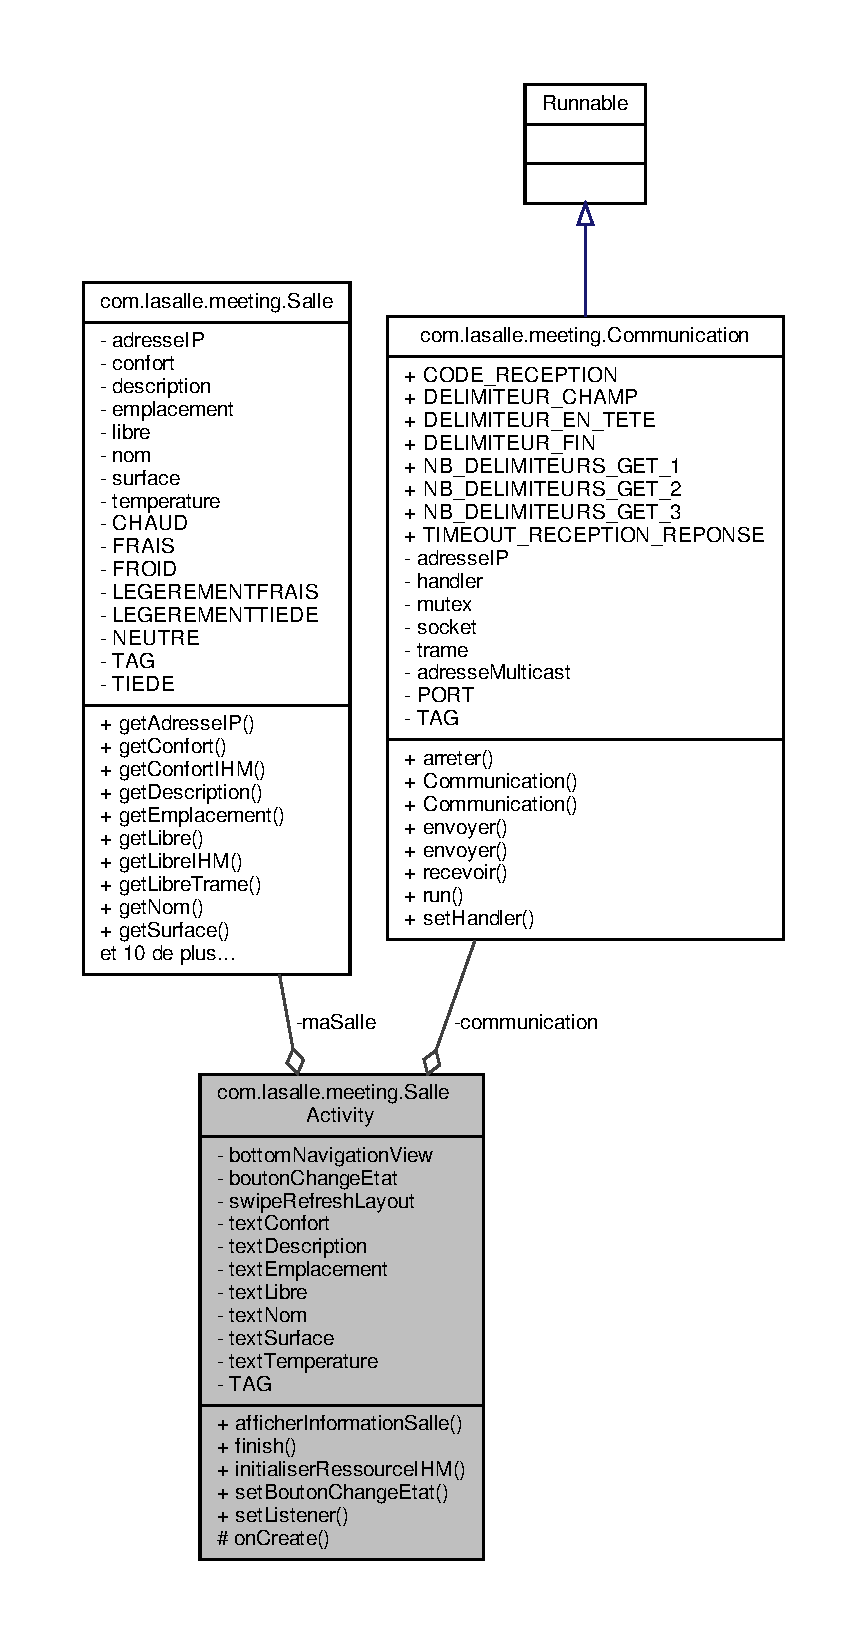
\includegraphics[height=550pt]{classcom_1_1lasalle_1_1meeting_1_1_salle_activity__coll__graph}
\end{center}
\end{figure}
\subsubsection*{Fonctions membres publiques}
\begin{DoxyCompactItemize}
\item 
void \hyperlink{classcom_1_1lasalle_1_1meeting_1_1_salle_activity_aee6f0cd7a9029d5fbe12bf85c2316f82}{afficher\+Information\+Salle} ()
\begin{DoxyCompactList}\small\item\em Méthode affichant les informations de la salle dans les layouts. \end{DoxyCompactList}\item 
void \hyperlink{classcom_1_1lasalle_1_1meeting_1_1_salle_activity_a26628d1f78ddcfaff36b33d354cd97b9}{finish} ()
\begin{DoxyCompactList}\small\item\em Méthode appelée à la fin de l\textquotesingle{}activité \hyperlink{classcom_1_1lasalle_1_1meeting_1_1_salle_activity}{Salle\+Activity}. \end{DoxyCompactList}\item 
void \hyperlink{classcom_1_1lasalle_1_1meeting_1_1_salle_activity_af41d9cf11c5032e1c44b7e8f08b8211a}{initialiser\+Ressource\+I\+HM} ()
\begin{DoxyCompactList}\small\item\em Récupère et initialise les widgets du layout activity\+\_\+salle. \end{DoxyCompactList}\item 
void \hyperlink{classcom_1_1lasalle_1_1meeting_1_1_salle_activity_a6b2086a70d8c1dc9841663029793ff00}{set\+Bouton\+Change\+Etat} ()
\begin{DoxyCompactList}\small\item\em Méthode changeant le bouton dépendant de la disponibilité de la salle. \end{DoxyCompactList}\item 
void \hyperlink{classcom_1_1lasalle_1_1meeting_1_1_salle_activity_a6d9b28a6a25b91ea9632ec4105dd33cf}{set\+Listener} ()
\begin{DoxyCompactList}\small\item\em applique les listener sur les layouts approprié \end{DoxyCompactList}\end{DoxyCompactItemize}
\subsubsection*{Fonctions membres protégées}
\begin{DoxyCompactItemize}
\item 
void \hyperlink{classcom_1_1lasalle_1_1meeting_1_1_salle_activity_a42079164af7344cb01a22eab03d2022f}{on\+Create} (Bundle saved\+Instance\+State)
\begin{DoxyCompactList}\small\item\em Méthode appelée à la création de l\textquotesingle{}activité \hyperlink{classcom_1_1lasalle_1_1meeting_1_1_salle_activity}{Salle\+Activity}. \end{DoxyCompactList}\end{DoxyCompactItemize}
\subsubsection*{Attributs privés}
\begin{DoxyCompactItemize}
\item 
Bottom\+Navigation\+View \hyperlink{classcom_1_1lasalle_1_1meeting_1_1_salle_activity_a43f122362683c363d7eee1b1f1dfd581}{bottom\+Navigation\+View}
\begin{DoxyCompactList}\small\item\em layout permettant d\textquotesingle{}avoir un menu de navigation (en haut) \end{DoxyCompactList}\item 
Button \hyperlink{classcom_1_1lasalle_1_1meeting_1_1_salle_activity_a0c33eac55429431e84849eca22ad3916}{bouton\+Change\+Etat}
\begin{DoxyCompactList}\small\item\em layout du prendre/liberer \end{DoxyCompactList}\item 
\hyperlink{classcom_1_1lasalle_1_1meeting_1_1_communication}{Communication} \hyperlink{classcom_1_1lasalle_1_1meeting_1_1_salle_activity_ab57d7397514ed7256304b0784f8ea7bf}{communication} = null
\begin{DoxyCompactList}\small\item\em attribut permetant d\textquotesingle{}envoyer des requêtes \end{DoxyCompactList}\item 
\hyperlink{classcom_1_1lasalle_1_1meeting_1_1_salle}{Salle} \hyperlink{classcom_1_1lasalle_1_1meeting_1_1_salle_activity_a7ae6e92ee66fa15d999f166f40738648}{ma\+Salle} = null
\begin{DoxyCompactList}\small\item\em attribut salle \end{DoxyCompactList}\item 
Swipe\+Refresh\+Layout \hyperlink{classcom_1_1lasalle_1_1meeting_1_1_salle_activity_aa331ece163b959f06fae00a637d37cb4}{swipe\+Refresh\+Layout}
\begin{DoxyCompactList}\small\item\em layout permettant de rafraichir \end{DoxyCompactList}\item 
Text\+View \hyperlink{classcom_1_1lasalle_1_1meeting_1_1_salle_activity_a9b647a7aaf2aab7a9e74cb525c250545}{text\+Confort}
\begin{DoxyCompactList}\small\item\em layout texte du confort de la salle \end{DoxyCompactList}\item 
Text\+View \hyperlink{classcom_1_1lasalle_1_1meeting_1_1_salle_activity_acc3b8d915861076b132cdc33f4d9f298}{text\+Description}
\begin{DoxyCompactList}\small\item\em layout texte de la description de la salle \end{DoxyCompactList}\item 
Text\+View \hyperlink{classcom_1_1lasalle_1_1meeting_1_1_salle_activity_a3e7b6e7c522546e84409d3b658985ca8}{text\+Emplacement}
\begin{DoxyCompactList}\small\item\em layout texte de l\textquotesingle{}emplacement de la salle \end{DoxyCompactList}\item 
Text\+View \hyperlink{classcom_1_1lasalle_1_1meeting_1_1_salle_activity_a3d80063be535c4f343498d1d0616092d}{text\+Libre}
\begin{DoxyCompactList}\small\item\em layout texte de la disponibilité de la salle \end{DoxyCompactList}\item 
Text\+View \hyperlink{classcom_1_1lasalle_1_1meeting_1_1_salle_activity_acb7acab3be7f76509ac3de29e715e008}{text\+Nom}
\begin{DoxyCompactList}\small\item\em layout texte du nom de la salle \end{DoxyCompactList}\item 
Text\+View \hyperlink{classcom_1_1lasalle_1_1meeting_1_1_salle_activity_a0fb3dcfded70ba78d8ce46a507ff7ef2}{text\+Surface}
\begin{DoxyCompactList}\small\item\em layout texte de la surface de la salle \end{DoxyCompactList}\item 
Text\+View \hyperlink{classcom_1_1lasalle_1_1meeting_1_1_salle_activity_a234ef25278aeb3164d379158fc294283}{text\+Temperature}
\begin{DoxyCompactList}\small\item\em layout texte de la température de la salle \end{DoxyCompactList}\end{DoxyCompactItemize}
\subsubsection*{Attributs privés statiques}
\begin{DoxyCompactItemize}
\item 
static final String \hyperlink{classcom_1_1lasalle_1_1meeting_1_1_salle_activity_a70adba176c2984edf5ae1b188017ac25}{T\+AG} = \char`\"{}Salle\+Activity\char`\"{}
\begin{DoxyCompactList}\small\item\em T\+AG utilisé pour les logs. \end{DoxyCompactList}\end{DoxyCompactItemize}


\subsubsection{Description détaillée}
Déclaration de la classe \hyperlink{classcom_1_1lasalle_1_1meeting_1_1_salle_activity}{Salle\+Activity}. 

Définition à la ligne \hyperlink{_salle_activity_8java_source_l00029}{29} du fichier \hyperlink{_salle_activity_8java_source}{Salle\+Activity.\+java}.



\subsubsection{Documentation des fonctions membres}
\mbox{\Hypertarget{classcom_1_1lasalle_1_1meeting_1_1_salle_activity_aee6f0cd7a9029d5fbe12bf85c2316f82}\label{classcom_1_1lasalle_1_1meeting_1_1_salle_activity_aee6f0cd7a9029d5fbe12bf85c2316f82}} 
\index{com\+::lasalle\+::meeting\+::\+Salle\+Activity@{com\+::lasalle\+::meeting\+::\+Salle\+Activity}!afficher\+Information\+Salle@{afficher\+Information\+Salle}}
\index{afficher\+Information\+Salle@{afficher\+Information\+Salle}!com\+::lasalle\+::meeting\+::\+Salle\+Activity@{com\+::lasalle\+::meeting\+::\+Salle\+Activity}}
\paragraph{\texorpdfstring{afficher\+Information\+Salle()}{afficherInformationSalle()}}
{\footnotesize\ttfamily void com.\+lasalle.\+meeting.\+Salle\+Activity.\+afficher\+Information\+Salle (\begin{DoxyParamCaption}{ }\end{DoxyParamCaption})}



Méthode affichant les informations de la salle dans les layouts. 

\begin{DoxyReturn}{Renvoie}
void 
\end{DoxyReturn}


Définition à la ligne \hyperlink{_salle_activity_8java_source_l00103}{103} du fichier \hyperlink{_salle_activity_8java_source}{Salle\+Activity.\+java}.



Références \hyperlink{_salle_8java_source_l00233}{com.\+lasalle.\+meeting.\+Salle.\+get\+Confort\+I\+H\+M()}, \hyperlink{_salle_8java_source_l00276}{com.\+lasalle.\+meeting.\+Salle.\+get\+Description()}, \hyperlink{_salle_8java_source_l00156}{com.\+lasalle.\+meeting.\+Salle.\+get\+Emplacement()}, \hyperlink{_salle_8java_source_l00174}{com.\+lasalle.\+meeting.\+Salle.\+get\+Libre()}, \hyperlink{_salle_8java_source_l00165}{com.\+lasalle.\+meeting.\+Salle.\+get\+Nom()}, \hyperlink{_salle_8java_source_l00215}{com.\+lasalle.\+meeting.\+Salle.\+get\+Surface()}, et \hyperlink{_salle_8java_source_l00267}{com.\+lasalle.\+meeting.\+Salle.\+get\+Temperature()}.



Référencé par \hyperlink{_salle_activity_8java_source_l00060}{com.\+lasalle.\+meeting.\+Salle\+Activity.\+on\+Create()}, et \hyperlink{_salle_activity_8java_source_l00132}{com.\+lasalle.\+meeting.\+Salle\+Activity.\+set\+Listener()}.


\begin{DoxyCode}
00104     \{
00105         \hyperlink{classcom_1_1lasalle_1_1meeting_1_1_salle_activity_acb7acab3be7f76509ac3de29e715e008}{textNom}.setText(\hyperlink{classcom_1_1lasalle_1_1meeting_1_1_salle_activity_a7ae6e92ee66fa15d999f166f40738648}{maSalle}.\hyperlink{classcom_1_1lasalle_1_1meeting_1_1_salle_a49d977f69b2783e8ad57eccffc29e97b}{getNom}());
00106         \hyperlink{classcom_1_1lasalle_1_1meeting_1_1_salle_activity_acb7acab3be7f76509ac3de29e715e008}{textNom}.setTextSize(35);
00107         \hyperlink{classcom_1_1lasalle_1_1meeting_1_1_salle_activity_acc3b8d915861076b132cdc33f4d9f298}{textDescription}.setText(\hyperlink{classcom_1_1lasalle_1_1meeting_1_1_salle_activity_a7ae6e92ee66fa15d999f166f40738648}{maSalle}.\hyperlink{classcom_1_1lasalle_1_1meeting_1_1_salle_a253315cc4da23a4b8ab092e10be6d13d}{getDescription}());
00108         \hyperlink{classcom_1_1lasalle_1_1meeting_1_1_salle_activity_acc3b8d915861076b132cdc33f4d9f298}{textDescription}.setTextSize(25);
00109         \hyperlink{classcom_1_1lasalle_1_1meeting_1_1_salle_activity_a3e7b6e7c522546e84409d3b658985ca8}{textEmplacement}.setText(\hyperlink{classcom_1_1lasalle_1_1meeting_1_1_salle_activity_a7ae6e92ee66fa15d999f166f40738648}{maSalle}.\hyperlink{classcom_1_1lasalle_1_1meeting_1_1_salle_ac58600d946b6553858cc41be032473cd}{getEmplacement}());
00110         \hyperlink{classcom_1_1lasalle_1_1meeting_1_1_salle_activity_a3e7b6e7c522546e84409d3b658985ca8}{textEmplacement}.setTextSize(25);
00111         \hyperlink{classcom_1_1lasalle_1_1meeting_1_1_salle_activity_a9b647a7aaf2aab7a9e74cb525c250545}{textConfort}.setText(\hyperlink{classcom_1_1lasalle_1_1meeting_1_1_salle_activity_a7ae6e92ee66fa15d999f166f40738648}{maSalle}.\hyperlink{classcom_1_1lasalle_1_1meeting_1_1_salle_abf1f96423a1df46ba4d6ac4a1b6d0c34}{getConfortIHM}());
00112         \hyperlink{classcom_1_1lasalle_1_1meeting_1_1_salle_activity_a9b647a7aaf2aab7a9e74cb525c250545}{textConfort}.setTextSize(25);
00113         \hyperlink{classcom_1_1lasalle_1_1meeting_1_1_salle_activity_a0fb3dcfded70ba78d8ce46a507ff7ef2}{textSurface}.setText(Integer.toString(\hyperlink{classcom_1_1lasalle_1_1meeting_1_1_salle_activity_a7ae6e92ee66fa15d999f166f40738648}{maSalle}.
      \hyperlink{classcom_1_1lasalle_1_1meeting_1_1_salle_ad9dad6b4cfeb020195d4cde268af885f}{getSurface}()) + \textcolor{stringliteral}{" m²"});
00114         \hyperlink{classcom_1_1lasalle_1_1meeting_1_1_salle_activity_a0fb3dcfded70ba78d8ce46a507ff7ef2}{textSurface}.setTextSize(25);
00115         \hyperlink{classcom_1_1lasalle_1_1meeting_1_1_salle_activity_a3d80063be535c4f343498d1d0616092d}{textLibre}.setTextSize(25);
00116         \textcolor{keywordflow}{if} (\hyperlink{classcom_1_1lasalle_1_1meeting_1_1_salle_activity_a7ae6e92ee66fa15d999f166f40738648}{maSalle}.\hyperlink{classcom_1_1lasalle_1_1meeting_1_1_salle_adc0c4936355bc0ae22991f69c12a5e42}{getLibre}() == \textcolor{keyword}{true})
00117         \{
00118             \hyperlink{classcom_1_1lasalle_1_1meeting_1_1_salle_activity_a3d80063be535c4f343498d1d0616092d}{textLibre}.setText(\textcolor{stringliteral}{"État : Libre"});
00119         \}
00120         \textcolor{keywordflow}{else}
00121         \{
00122             \hyperlink{classcom_1_1lasalle_1_1meeting_1_1_salle_activity_a3d80063be535c4f343498d1d0616092d}{textLibre}.setText(\textcolor{stringliteral}{"État : Occupée"});
00123         \}
00124         \hyperlink{classcom_1_1lasalle_1_1meeting_1_1_salle_activity_a234ef25278aeb3164d379158fc294283}{textTemperature}.setText(Float.toString(\hyperlink{classcom_1_1lasalle_1_1meeting_1_1_salle_activity_a7ae6e92ee66fa15d999f166f40738648}{maSalle}.
      \hyperlink{classcom_1_1lasalle_1_1meeting_1_1_salle_ae3235f548f8bc7ab4d05ff38ec762e77}{getTemperature}()) + \textcolor{stringliteral}{" °C"});
00125         \hyperlink{classcom_1_1lasalle_1_1meeting_1_1_salle_activity_a234ef25278aeb3164d379158fc294283}{textTemperature}.setTextSize(25);
00126     \}
\end{DoxyCode}
\mbox{\Hypertarget{classcom_1_1lasalle_1_1meeting_1_1_salle_activity_a26628d1f78ddcfaff36b33d354cd97b9}\label{classcom_1_1lasalle_1_1meeting_1_1_salle_activity_a26628d1f78ddcfaff36b33d354cd97b9}} 
\index{com\+::lasalle\+::meeting\+::\+Salle\+Activity@{com\+::lasalle\+::meeting\+::\+Salle\+Activity}!finish@{finish}}
\index{finish@{finish}!com\+::lasalle\+::meeting\+::\+Salle\+Activity@{com\+::lasalle\+::meeting\+::\+Salle\+Activity}}
\paragraph{\texorpdfstring{finish()}{finish()}}
{\footnotesize\ttfamily void com.\+lasalle.\+meeting.\+Salle\+Activity.\+finish (\begin{DoxyParamCaption}{ }\end{DoxyParamCaption})}



Méthode appelée à la fin de l\textquotesingle{}activité \hyperlink{classcom_1_1lasalle_1_1meeting_1_1_salle_activity}{Salle\+Activity}. 

\begin{DoxyReturn}{Renvoie}
void 
\end{DoxyReturn}


Définition à la ligne \hyperlink{_salle_activity_8java_source_l00208}{208} du fichier \hyperlink{_salle_activity_8java_source}{Salle\+Activity.\+java}.


\begin{DoxyCode}
00209     \{
00210         Log.d(\hyperlink{classcom_1_1lasalle_1_1meeting_1_1_salle_activity_a70adba176c2984edf5ae1b188017ac25}{TAG}, \textcolor{stringliteral}{"finish()"});
00211 
00212         Intent intent = \textcolor{keyword}{new} Intent();
00213 
00214         intent.putExtra(\textcolor{stringliteral}{"salle"}, \hyperlink{classcom_1_1lasalle_1_1meeting_1_1_salle_activity_a7ae6e92ee66fa15d999f166f40738648}{maSalle});
00215 
00216         setResult(RESULT\_OK, intent);
00217         super.finish();
00218     \}
\end{DoxyCode}
\mbox{\Hypertarget{classcom_1_1lasalle_1_1meeting_1_1_salle_activity_af41d9cf11c5032e1c44b7e8f08b8211a}\label{classcom_1_1lasalle_1_1meeting_1_1_salle_activity_af41d9cf11c5032e1c44b7e8f08b8211a}} 
\index{com\+::lasalle\+::meeting\+::\+Salle\+Activity@{com\+::lasalle\+::meeting\+::\+Salle\+Activity}!initialiser\+Ressource\+I\+HM@{initialiser\+Ressource\+I\+HM}}
\index{initialiser\+Ressource\+I\+HM@{initialiser\+Ressource\+I\+HM}!com\+::lasalle\+::meeting\+::\+Salle\+Activity@{com\+::lasalle\+::meeting\+::\+Salle\+Activity}}
\paragraph{\texorpdfstring{initialiser\+Ressource\+I\+H\+M()}{initialiserRessourceIHM()}}
{\footnotesize\ttfamily void com.\+lasalle.\+meeting.\+Salle\+Activity.\+initialiser\+Ressource\+I\+HM (\begin{DoxyParamCaption}{ }\end{DoxyParamCaption})}



Récupère et initialise les widgets du layout activity\+\_\+salle. 

\begin{DoxyReturn}{Renvoie}
void 
\end{DoxyReturn}


Définition à la ligne \hyperlink{_salle_activity_8java_source_l00189}{189} du fichier \hyperlink{_salle_activity_8java_source}{Salle\+Activity.\+java}.



Référencé par \hyperlink{_salle_activity_8java_source_l00060}{com.\+lasalle.\+meeting.\+Salle\+Activity.\+on\+Create()}.


\begin{DoxyCode}
00190     \{
00191         \hyperlink{classcom_1_1lasalle_1_1meeting_1_1_salle_activity_a0c33eac55429431e84849eca22ad3916}{boutonChangeEtat} = (Button)findViewById(R.id.buttonChangeEtat);
00192         \hyperlink{classcom_1_1lasalle_1_1meeting_1_1_salle_activity_acb7acab3be7f76509ac3de29e715e008}{textNom} = (TextView)findViewById(R.id.textViewNom);
00193         \hyperlink{classcom_1_1lasalle_1_1meeting_1_1_salle_activity_a3e7b6e7c522546e84409d3b658985ca8}{textEmplacement} = (TextView)findViewById(R.id.textViewEmplacement);
00194         \hyperlink{classcom_1_1lasalle_1_1meeting_1_1_salle_activity_a3d80063be535c4f343498d1d0616092d}{textLibre} = (TextView)findViewById(R.id.textViewLibre);
00195         \hyperlink{classcom_1_1lasalle_1_1meeting_1_1_salle_activity_a9b647a7aaf2aab7a9e74cb525c250545}{textConfort} = (TextView)findViewById(R.id.textViewConfort);
00196         \hyperlink{classcom_1_1lasalle_1_1meeting_1_1_salle_activity_a0fb3dcfded70ba78d8ce46a507ff7ef2}{textSurface} = (TextView)findViewById(R.id.textViewSurface);
00197         \hyperlink{classcom_1_1lasalle_1_1meeting_1_1_salle_activity_a234ef25278aeb3164d379158fc294283}{textTemperature} = (TextView)findViewById(R.id.textViewTemperature);
00198         \hyperlink{classcom_1_1lasalle_1_1meeting_1_1_salle_activity_acc3b8d915861076b132cdc33f4d9f298}{textDescription} = (TextView)findViewById(R.id.textViewDescription);
00199         \hyperlink{classcom_1_1lasalle_1_1meeting_1_1_salle_activity_aa331ece163b959f06fae00a637d37cb4}{swipeRefreshLayout} = (SwipeRefreshLayout)findViewById(R.id.swipeRefreshLayout);
00200         \hyperlink{classcom_1_1lasalle_1_1meeting_1_1_salle_activity_a43f122362683c363d7eee1b1f1dfd581}{bottomNavigationView} = (BottomNavigationView) findViewById(R.id.
      bottomNavigationView);
00201     \}
\end{DoxyCode}
\mbox{\Hypertarget{classcom_1_1lasalle_1_1meeting_1_1_salle_activity_a42079164af7344cb01a22eab03d2022f}\label{classcom_1_1lasalle_1_1meeting_1_1_salle_activity_a42079164af7344cb01a22eab03d2022f}} 
\index{com\+::lasalle\+::meeting\+::\+Salle\+Activity@{com\+::lasalle\+::meeting\+::\+Salle\+Activity}!on\+Create@{on\+Create}}
\index{on\+Create@{on\+Create}!com\+::lasalle\+::meeting\+::\+Salle\+Activity@{com\+::lasalle\+::meeting\+::\+Salle\+Activity}}
\paragraph{\texorpdfstring{on\+Create()}{onCreate()}}
{\footnotesize\ttfamily void com.\+lasalle.\+meeting.\+Salle\+Activity.\+on\+Create (\begin{DoxyParamCaption}\item[{Bundle}]{saved\+Instance\+State }\end{DoxyParamCaption})\hspace{0.3cm}{\ttfamily [protected]}}



Méthode appelée à la création de l\textquotesingle{}activité \hyperlink{classcom_1_1lasalle_1_1meeting_1_1_salle_activity}{Salle\+Activity}. 


\begin{DoxyParams}{Paramètres}
{\em saved\+Instance\+State} & \\
\hline
\end{DoxyParams}
\begin{DoxyReturn}{Renvoie}
void 
\end{DoxyReturn}


Définition à la ligne \hyperlink{_salle_activity_8java_source_l00060}{60} du fichier \hyperlink{_salle_activity_8java_source}{Salle\+Activity.\+java}.



Références \hyperlink{_salle_activity_8java_source_l00103}{com.\+lasalle.\+meeting.\+Salle\+Activity.\+afficher\+Information\+Salle()}, \hyperlink{_main_activity_8java_source_l00479}{com.\+lasalle.\+meeting.\+Main\+Activity.\+get\+Communication()}, \hyperlink{_salle_8java_source_l00165}{com.\+lasalle.\+meeting.\+Salle.\+get\+Nom()}, \hyperlink{_salle_activity_8java_source_l00189}{com.\+lasalle.\+meeting.\+Salle\+Activity.\+initialiser\+Ressource\+I\+H\+M()}, \hyperlink{_salle_activity_8java_source_l00085}{com.\+lasalle.\+meeting.\+Salle\+Activity.\+set\+Bouton\+Change\+Etat()}, et \hyperlink{_salle_activity_8java_source_l00132}{com.\+lasalle.\+meeting.\+Salle\+Activity.\+set\+Listener()}.


\begin{DoxyCode}
00061     \{
00062         super.onCreate(savedInstanceState);
00063         Log.d(\hyperlink{classcom_1_1lasalle_1_1meeting_1_1_salle_activity_a70adba176c2984edf5ae1b188017ac25}{TAG}, \textcolor{stringliteral}{"onCreate()"});
00064 
00065         setContentView(R.layout.activity\_salle);
00066 
00067         Intent intent = getIntent();
00068         \hyperlink{classcom_1_1lasalle_1_1meeting_1_1_salle_activity_a7ae6e92ee66fa15d999f166f40738648}{maSalle} = (Salle)intent.getSerializableExtra(\textcolor{stringliteral}{"Salle"});
00069 
00070         \textcolor{keywordflow}{if}(\hyperlink{classcom_1_1lasalle_1_1meeting_1_1_salle_activity_a7ae6e92ee66fa15d999f166f40738648}{maSalle} == null)
00071             Log.d(\hyperlink{classcom_1_1lasalle_1_1meeting_1_1_salle_activity_a70adba176c2984edf5ae1b188017ac25}{TAG}, \textcolor{stringliteral}{"Salle : "} + \hyperlink{classcom_1_1lasalle_1_1meeting_1_1_salle_activity_a7ae6e92ee66fa15d999f166f40738648}{maSalle}.\hyperlink{classcom_1_1lasalle_1_1meeting_1_1_salle_a49d977f69b2783e8ad57eccffc29e97b}{getNom}());
00072 
00073         \hyperlink{classcom_1_1lasalle_1_1meeting_1_1_salle_activity_ab57d7397514ed7256304b0784f8ea7bf}{communication} = MainActivity.getCommunication();
00074 
00075         \hyperlink{classcom_1_1lasalle_1_1meeting_1_1_salle_activity_af41d9cf11c5032e1c44b7e8f08b8211a}{initialiserRessourceIHM}();
00076         \hyperlink{classcom_1_1lasalle_1_1meeting_1_1_salle_activity_a6b2086a70d8c1dc9841663029793ff00}{setBoutonChangeEtat}();
00077         \hyperlink{classcom_1_1lasalle_1_1meeting_1_1_salle_activity_aee6f0cd7a9029d5fbe12bf85c2316f82}{afficherInformationSalle}();
00078         \hyperlink{classcom_1_1lasalle_1_1meeting_1_1_salle_activity_a6d9b28a6a25b91ea9632ec4105dd33cf}{setListener}();
00079     \}
\end{DoxyCode}
\mbox{\Hypertarget{classcom_1_1lasalle_1_1meeting_1_1_salle_activity_a6b2086a70d8c1dc9841663029793ff00}\label{classcom_1_1lasalle_1_1meeting_1_1_salle_activity_a6b2086a70d8c1dc9841663029793ff00}} 
\index{com\+::lasalle\+::meeting\+::\+Salle\+Activity@{com\+::lasalle\+::meeting\+::\+Salle\+Activity}!set\+Bouton\+Change\+Etat@{set\+Bouton\+Change\+Etat}}
\index{set\+Bouton\+Change\+Etat@{set\+Bouton\+Change\+Etat}!com\+::lasalle\+::meeting\+::\+Salle\+Activity@{com\+::lasalle\+::meeting\+::\+Salle\+Activity}}
\paragraph{\texorpdfstring{set\+Bouton\+Change\+Etat()}{setBoutonChangeEtat()}}
{\footnotesize\ttfamily void com.\+lasalle.\+meeting.\+Salle\+Activity.\+set\+Bouton\+Change\+Etat (\begin{DoxyParamCaption}{ }\end{DoxyParamCaption})}



Méthode changeant le bouton dépendant de la disponibilité de la salle. 

\begin{DoxyReturn}{Renvoie}
void 
\end{DoxyReturn}


Définition à la ligne \hyperlink{_salle_activity_8java_source_l00085}{85} du fichier \hyperlink{_salle_activity_8java_source}{Salle\+Activity.\+java}.



Références \hyperlink{_salle_8java_source_l00174}{com.\+lasalle.\+meeting.\+Salle.\+get\+Libre()}.



Référencé par \hyperlink{_salle_activity_8java_source_l00060}{com.\+lasalle.\+meeting.\+Salle\+Activity.\+on\+Create()}, et \hyperlink{_salle_activity_8java_source_l00132}{com.\+lasalle.\+meeting.\+Salle\+Activity.\+set\+Listener()}.


\begin{DoxyCode}
00086     \{
00087         \textcolor{keywordflow}{if} (\hyperlink{classcom_1_1lasalle_1_1meeting_1_1_salle_activity_a7ae6e92ee66fa15d999f166f40738648}{maSalle}.\hyperlink{classcom_1_1lasalle_1_1meeting_1_1_salle_adc0c4936355bc0ae22991f69c12a5e42}{getLibre}() == \textcolor{keyword}{true})
00088         \{
00089             \hyperlink{classcom_1_1lasalle_1_1meeting_1_1_salle_activity_a0c33eac55429431e84849eca22ad3916}{boutonChangeEtat}.setText(\textcolor{stringliteral}{"Prendre"});
00090             \hyperlink{classcom_1_1lasalle_1_1meeting_1_1_salle_activity_a0c33eac55429431e84849eca22ad3916}{boutonChangeEtat}.setBackgroundColor(Color.rgb(39,195,26));
00091         \}
00092         \textcolor{keywordflow}{else}
00093         \{
00094             \hyperlink{classcom_1_1lasalle_1_1meeting_1_1_salle_activity_a0c33eac55429431e84849eca22ad3916}{boutonChangeEtat}.setText(\textcolor{stringliteral}{"Libérer"});
00095             \hyperlink{classcom_1_1lasalle_1_1meeting_1_1_salle_activity_a0c33eac55429431e84849eca22ad3916}{boutonChangeEtat}.setBackgroundColor(Color.rgb(222,55,25));
00096         \}
00097     \}
\end{DoxyCode}
\mbox{\Hypertarget{classcom_1_1lasalle_1_1meeting_1_1_salle_activity_a6d9b28a6a25b91ea9632ec4105dd33cf}\label{classcom_1_1lasalle_1_1meeting_1_1_salle_activity_a6d9b28a6a25b91ea9632ec4105dd33cf}} 
\index{com\+::lasalle\+::meeting\+::\+Salle\+Activity@{com\+::lasalle\+::meeting\+::\+Salle\+Activity}!set\+Listener@{set\+Listener}}
\index{set\+Listener@{set\+Listener}!com\+::lasalle\+::meeting\+::\+Salle\+Activity@{com\+::lasalle\+::meeting\+::\+Salle\+Activity}}
\paragraph{\texorpdfstring{set\+Listener()}{setListener()}}
{\footnotesize\ttfamily void com.\+lasalle.\+meeting.\+Salle\+Activity.\+set\+Listener (\begin{DoxyParamCaption}{ }\end{DoxyParamCaption})}



applique les listener sur les layouts approprié 

\begin{DoxyReturn}{Renvoie}
void 
\end{DoxyReturn}


Définition à la ligne \hyperlink{_salle_activity_8java_source_l00132}{132} du fichier \hyperlink{_salle_activity_8java_source}{Salle\+Activity.\+java}.



Références \hyperlink{_salle_activity_8java_source_l00103}{com.\+lasalle.\+meeting.\+Salle\+Activity.\+afficher\+Information\+Salle()}, \hyperlink{_communication_8java_source_l00161}{com.\+lasalle.\+meeting.\+Communication.\+envoyer()}, \hyperlink{_salle_8java_source_l00285}{com.\+lasalle.\+meeting.\+Salle.\+get\+Adresse\+I\+P()}, \hyperlink{_salle_8java_source_l00183}{com.\+lasalle.\+meeting.\+Salle.\+get\+Libre\+Trame()}, \hyperlink{_salle_activity_8java_source_l00085}{com.\+lasalle.\+meeting.\+Salle\+Activity.\+set\+Bouton\+Change\+Etat()}, et \hyperlink{_salle_8java_source_l00089}{com.\+lasalle.\+meeting.\+Salle.\+set\+Libre()}.



Référencé par \hyperlink{_salle_activity_8java_source_l00060}{com.\+lasalle.\+meeting.\+Salle\+Activity.\+on\+Create()}.


\begin{DoxyCode}
00133     \{
00134 
00135         \hyperlink{classcom_1_1lasalle_1_1meeting_1_1_salle_activity_a0c33eac55429431e84849eca22ad3916}{boutonChangeEtat}.setOnClickListener(
00136                 \textcolor{keyword}{new} View.OnClickListener()
00137                 \{
00138                     @Override
00139                     \textcolor{keyword}{public} \textcolor{keywordtype}{void} onClick(View v)
00140                     \{
00141                         \hyperlink{classcom_1_1lasalle_1_1meeting_1_1_salle_activity_a7ae6e92ee66fa15d999f166f40738648}{maSalle}.\hyperlink{classcom_1_1lasalle_1_1meeting_1_1_salle_a94c64624d647ec3ec60a9fbeb06948b8}{setLibre}();
00142                         \hyperlink{classcom_1_1lasalle_1_1meeting_1_1_salle_activity_a6b2086a70d8c1dc9841663029793ff00}{setBoutonChangeEtat}();
00143                         \hyperlink{classcom_1_1lasalle_1_1meeting_1_1_salle_activity_aee6f0cd7a9029d5fbe12bf85c2316f82}{afficherInformationSalle}();
00144 
00145                         \textcolor{keywordflow}{if}(\hyperlink{classcom_1_1lasalle_1_1meeting_1_1_salle_activity_ab57d7397514ed7256304b0784f8ea7bf}{communication} != null)
00146                         \{
00147                             \hyperlink{classcom_1_1lasalle_1_1meeting_1_1_salle_activity_ab57d7397514ed7256304b0784f8ea7bf}{communication}.\hyperlink{classcom_1_1lasalle_1_1meeting_1_1_communication_a1566200ca56ba63eec13d0ce37e6c7ee}{envoyer}(\textcolor{stringliteral}{"$SET;3;"} + 
      \hyperlink{classcom_1_1lasalle_1_1meeting_1_1_salle_activity_a7ae6e92ee66fa15d999f166f40738648}{maSalle}.\hyperlink{classcom_1_1lasalle_1_1meeting_1_1_salle_a0039fabf5867aef87f5f61f0081bcbcd}{getLibreTrame}() + \textcolor{stringliteral}{"\(\backslash\)r\(\backslash\)n"}, \hyperlink{classcom_1_1lasalle_1_1meeting_1_1_salle_activity_a7ae6e92ee66fa15d999f166f40738648}{maSalle}.
      \hyperlink{classcom_1_1lasalle_1_1meeting_1_1_salle_a2189e9d589972421a0f57d045471caa8}{getAdresseIP}());
00148                         \}
00149                     \}
00150                 \}
00151         );
00152 
00153         \hyperlink{classcom_1_1lasalle_1_1meeting_1_1_salle_activity_aa331ece163b959f06fae00a637d37cb4}{swipeRefreshLayout}.setOnRefreshListener(\textcolor{keyword}{new} SwipeRefreshLayout.OnRefreshListener(
      )
00154         \{
00155             @Override
00156             \textcolor{keyword}{public} \textcolor{keywordtype}{void} onRefresh()
00157             \{
00158                 \hyperlink{classcom_1_1lasalle_1_1meeting_1_1_salle_activity_aee6f0cd7a9029d5fbe12bf85c2316f82}{afficherInformationSalle}();
00159                 \hyperlink{classcom_1_1lasalle_1_1meeting_1_1_salle_activity_aa331ece163b959f06fae00a637d37cb4}{swipeRefreshLayout}.setRefreshing(\textcolor{keyword}{false});
00160             \}
00161         \});
00162 
00163         \hyperlink{classcom_1_1lasalle_1_1meeting_1_1_salle_activity_a43f122362683c363d7eee1b1f1dfd581}{bottomNavigationView}.setOnNavigationItemSelectedListener(\textcolor{keyword}{new} 
      BottomNavigationView.OnNavigationItemSelectedListener()
00164         \{
00165             @Override
00166             \textcolor{keyword}{public} \textcolor{keywordtype}{boolean} onNavigationItemSelected(@NonNull MenuItem item)
00167             \{
00168                 \textcolor{keywordflow}{switch} (item.getItemId())
00169                 \{
00170                     \textcolor{keywordflow}{case} R.id.Salle:
00171                         Toast.makeText(getApplicationContext(), \textcolor{stringliteral}{"Salle"}, Toast.LENGTH\_SHORT).show();
00172                         \textcolor{keywordflow}{return} \textcolor{keyword}{true};
00173                     \textcolor{keywordflow}{case} R.id.Favoris:
00174                         Toast.makeText(getApplicationContext(), \textcolor{stringliteral}{"La fonctionnalité favoris n'est pas encore
       disponible !"}, Toast.LENGTH\_SHORT).show();
00175                         \textcolor{keywordflow}{return} \textcolor{keyword}{true};
00176                     \textcolor{keywordflow}{case} R.id.Rechercher:
00177                         Toast.makeText(getApplicationContext(), \textcolor{stringliteral}{"La fonctionnalité rechercher n'est pas
       encore disponible !"}, Toast.LENGTH\_SHORT).show();
00178                         \textcolor{keywordflow}{return} \textcolor{keyword}{true};
00179                 \}
00180                 \textcolor{keywordflow}{return} \textcolor{keyword}{false};
00181             \}
00182         \});
00183     \}
\end{DoxyCode}


\subsubsection{Documentation des données membres}
\mbox{\Hypertarget{classcom_1_1lasalle_1_1meeting_1_1_salle_activity_a43f122362683c363d7eee1b1f1dfd581}\label{classcom_1_1lasalle_1_1meeting_1_1_salle_activity_a43f122362683c363d7eee1b1f1dfd581}} 
\index{com\+::lasalle\+::meeting\+::\+Salle\+Activity@{com\+::lasalle\+::meeting\+::\+Salle\+Activity}!bottom\+Navigation\+View@{bottom\+Navigation\+View}}
\index{bottom\+Navigation\+View@{bottom\+Navigation\+View}!com\+::lasalle\+::meeting\+::\+Salle\+Activity@{com\+::lasalle\+::meeting\+::\+Salle\+Activity}}
\paragraph{\texorpdfstring{bottom\+Navigation\+View}{bottomNavigationView}}
{\footnotesize\ttfamily Bottom\+Navigation\+View com.\+lasalle.\+meeting.\+Salle\+Activity.\+bottom\+Navigation\+View\hspace{0.3cm}{\ttfamily [private]}}



layout permettant d\textquotesingle{}avoir un menu de navigation (en haut) 



Définition à la ligne \hyperlink{_salle_activity_8java_source_l00047}{47} du fichier \hyperlink{_salle_activity_8java_source}{Salle\+Activity.\+java}.

\mbox{\Hypertarget{classcom_1_1lasalle_1_1meeting_1_1_salle_activity_a0c33eac55429431e84849eca22ad3916}\label{classcom_1_1lasalle_1_1meeting_1_1_salle_activity_a0c33eac55429431e84849eca22ad3916}} 
\index{com\+::lasalle\+::meeting\+::\+Salle\+Activity@{com\+::lasalle\+::meeting\+::\+Salle\+Activity}!bouton\+Change\+Etat@{bouton\+Change\+Etat}}
\index{bouton\+Change\+Etat@{bouton\+Change\+Etat}!com\+::lasalle\+::meeting\+::\+Salle\+Activity@{com\+::lasalle\+::meeting\+::\+Salle\+Activity}}
\paragraph{\texorpdfstring{bouton\+Change\+Etat}{boutonChangeEtat}}
{\footnotesize\ttfamily Button com.\+lasalle.\+meeting.\+Salle\+Activity.\+bouton\+Change\+Etat\hspace{0.3cm}{\ttfamily [private]}}



layout du prendre/liberer 

Ressources layout activity\+\_\+main 

Définition à la ligne \hyperlink{_salle_activity_8java_source_l00038}{38} du fichier \hyperlink{_salle_activity_8java_source}{Salle\+Activity.\+java}.

\mbox{\Hypertarget{classcom_1_1lasalle_1_1meeting_1_1_salle_activity_ab57d7397514ed7256304b0784f8ea7bf}\label{classcom_1_1lasalle_1_1meeting_1_1_salle_activity_ab57d7397514ed7256304b0784f8ea7bf}} 
\index{com\+::lasalle\+::meeting\+::\+Salle\+Activity@{com\+::lasalle\+::meeting\+::\+Salle\+Activity}!communication@{communication}}
\index{communication@{communication}!com\+::lasalle\+::meeting\+::\+Salle\+Activity@{com\+::lasalle\+::meeting\+::\+Salle\+Activity}}
\paragraph{\texorpdfstring{communication}{communication}}
{\footnotesize\ttfamily \hyperlink{classcom_1_1lasalle_1_1meeting_1_1_communication}{Communication} com.\+lasalle.\+meeting.\+Salle\+Activity.\+communication = null\hspace{0.3cm}{\ttfamily [private]}}



attribut permetant d\textquotesingle{}envoyer des requêtes 



Définition à la ligne \hyperlink{_salle_activity_8java_source_l00052}{52} du fichier \hyperlink{_salle_activity_8java_source}{Salle\+Activity.\+java}.

\mbox{\Hypertarget{classcom_1_1lasalle_1_1meeting_1_1_salle_activity_a7ae6e92ee66fa15d999f166f40738648}\label{classcom_1_1lasalle_1_1meeting_1_1_salle_activity_a7ae6e92ee66fa15d999f166f40738648}} 
\index{com\+::lasalle\+::meeting\+::\+Salle\+Activity@{com\+::lasalle\+::meeting\+::\+Salle\+Activity}!ma\+Salle@{ma\+Salle}}
\index{ma\+Salle@{ma\+Salle}!com\+::lasalle\+::meeting\+::\+Salle\+Activity@{com\+::lasalle\+::meeting\+::\+Salle\+Activity}}
\paragraph{\texorpdfstring{ma\+Salle}{maSalle}}
{\footnotesize\ttfamily \hyperlink{classcom_1_1lasalle_1_1meeting_1_1_salle}{Salle} com.\+lasalle.\+meeting.\+Salle\+Activity.\+ma\+Salle = null\hspace{0.3cm}{\ttfamily [private]}}



attribut salle 

Attributs 

Définition à la ligne \hyperlink{_salle_activity_8java_source_l00051}{51} du fichier \hyperlink{_salle_activity_8java_source}{Salle\+Activity.\+java}.

\mbox{\Hypertarget{classcom_1_1lasalle_1_1meeting_1_1_salle_activity_aa331ece163b959f06fae00a637d37cb4}\label{classcom_1_1lasalle_1_1meeting_1_1_salle_activity_aa331ece163b959f06fae00a637d37cb4}} 
\index{com\+::lasalle\+::meeting\+::\+Salle\+Activity@{com\+::lasalle\+::meeting\+::\+Salle\+Activity}!swipe\+Refresh\+Layout@{swipe\+Refresh\+Layout}}
\index{swipe\+Refresh\+Layout@{swipe\+Refresh\+Layout}!com\+::lasalle\+::meeting\+::\+Salle\+Activity@{com\+::lasalle\+::meeting\+::\+Salle\+Activity}}
\paragraph{\texorpdfstring{swipe\+Refresh\+Layout}{swipeRefreshLayout}}
{\footnotesize\ttfamily Swipe\+Refresh\+Layout com.\+lasalle.\+meeting.\+Salle\+Activity.\+swipe\+Refresh\+Layout\hspace{0.3cm}{\ttfamily [private]}}



layout permettant de rafraichir 



Définition à la ligne \hyperlink{_salle_activity_8java_source_l00046}{46} du fichier \hyperlink{_salle_activity_8java_source}{Salle\+Activity.\+java}.

\mbox{\Hypertarget{classcom_1_1lasalle_1_1meeting_1_1_salle_activity_a70adba176c2984edf5ae1b188017ac25}\label{classcom_1_1lasalle_1_1meeting_1_1_salle_activity_a70adba176c2984edf5ae1b188017ac25}} 
\index{com\+::lasalle\+::meeting\+::\+Salle\+Activity@{com\+::lasalle\+::meeting\+::\+Salle\+Activity}!T\+AG@{T\+AG}}
\index{T\+AG@{T\+AG}!com\+::lasalle\+::meeting\+::\+Salle\+Activity@{com\+::lasalle\+::meeting\+::\+Salle\+Activity}}
\paragraph{\texorpdfstring{T\+AG}{TAG}}
{\footnotesize\ttfamily final String com.\+lasalle.\+meeting.\+Salle\+Activity.\+T\+AG = \char`\"{}Salle\+Activity\char`\"{}\hspace{0.3cm}{\ttfamily [static]}, {\ttfamily [private]}}



T\+AG utilisé pour les logs. 

Constantes 

Définition à la ligne \hyperlink{_salle_activity_8java_source_l00034}{34} du fichier \hyperlink{_salle_activity_8java_source}{Salle\+Activity.\+java}.

\mbox{\Hypertarget{classcom_1_1lasalle_1_1meeting_1_1_salle_activity_a9b647a7aaf2aab7a9e74cb525c250545}\label{classcom_1_1lasalle_1_1meeting_1_1_salle_activity_a9b647a7aaf2aab7a9e74cb525c250545}} 
\index{com\+::lasalle\+::meeting\+::\+Salle\+Activity@{com\+::lasalle\+::meeting\+::\+Salle\+Activity}!text\+Confort@{text\+Confort}}
\index{text\+Confort@{text\+Confort}!com\+::lasalle\+::meeting\+::\+Salle\+Activity@{com\+::lasalle\+::meeting\+::\+Salle\+Activity}}
\paragraph{\texorpdfstring{text\+Confort}{textConfort}}
{\footnotesize\ttfamily Text\+View com.\+lasalle.\+meeting.\+Salle\+Activity.\+text\+Confort\hspace{0.3cm}{\ttfamily [private]}}



layout texte du confort de la salle 



Définition à la ligne \hyperlink{_salle_activity_8java_source_l00042}{42} du fichier \hyperlink{_salle_activity_8java_source}{Salle\+Activity.\+java}.

\mbox{\Hypertarget{classcom_1_1lasalle_1_1meeting_1_1_salle_activity_acc3b8d915861076b132cdc33f4d9f298}\label{classcom_1_1lasalle_1_1meeting_1_1_salle_activity_acc3b8d915861076b132cdc33f4d9f298}} 
\index{com\+::lasalle\+::meeting\+::\+Salle\+Activity@{com\+::lasalle\+::meeting\+::\+Salle\+Activity}!text\+Description@{text\+Description}}
\index{text\+Description@{text\+Description}!com\+::lasalle\+::meeting\+::\+Salle\+Activity@{com\+::lasalle\+::meeting\+::\+Salle\+Activity}}
\paragraph{\texorpdfstring{text\+Description}{textDescription}}
{\footnotesize\ttfamily Text\+View com.\+lasalle.\+meeting.\+Salle\+Activity.\+text\+Description\hspace{0.3cm}{\ttfamily [private]}}



layout texte de la description de la salle 



Définition à la ligne \hyperlink{_salle_activity_8java_source_l00045}{45} du fichier \hyperlink{_salle_activity_8java_source}{Salle\+Activity.\+java}.

\mbox{\Hypertarget{classcom_1_1lasalle_1_1meeting_1_1_salle_activity_a3e7b6e7c522546e84409d3b658985ca8}\label{classcom_1_1lasalle_1_1meeting_1_1_salle_activity_a3e7b6e7c522546e84409d3b658985ca8}} 
\index{com\+::lasalle\+::meeting\+::\+Salle\+Activity@{com\+::lasalle\+::meeting\+::\+Salle\+Activity}!text\+Emplacement@{text\+Emplacement}}
\index{text\+Emplacement@{text\+Emplacement}!com\+::lasalle\+::meeting\+::\+Salle\+Activity@{com\+::lasalle\+::meeting\+::\+Salle\+Activity}}
\paragraph{\texorpdfstring{text\+Emplacement}{textEmplacement}}
{\footnotesize\ttfamily Text\+View com.\+lasalle.\+meeting.\+Salle\+Activity.\+text\+Emplacement\hspace{0.3cm}{\ttfamily [private]}}



layout texte de l\textquotesingle{}emplacement de la salle 



Définition à la ligne \hyperlink{_salle_activity_8java_source_l00040}{40} du fichier \hyperlink{_salle_activity_8java_source}{Salle\+Activity.\+java}.

\mbox{\Hypertarget{classcom_1_1lasalle_1_1meeting_1_1_salle_activity_a3d80063be535c4f343498d1d0616092d}\label{classcom_1_1lasalle_1_1meeting_1_1_salle_activity_a3d80063be535c4f343498d1d0616092d}} 
\index{com\+::lasalle\+::meeting\+::\+Salle\+Activity@{com\+::lasalle\+::meeting\+::\+Salle\+Activity}!text\+Libre@{text\+Libre}}
\index{text\+Libre@{text\+Libre}!com\+::lasalle\+::meeting\+::\+Salle\+Activity@{com\+::lasalle\+::meeting\+::\+Salle\+Activity}}
\paragraph{\texorpdfstring{text\+Libre}{textLibre}}
{\footnotesize\ttfamily Text\+View com.\+lasalle.\+meeting.\+Salle\+Activity.\+text\+Libre\hspace{0.3cm}{\ttfamily [private]}}



layout texte de la disponibilité de la salle 



Définition à la ligne \hyperlink{_salle_activity_8java_source_l00041}{41} du fichier \hyperlink{_salle_activity_8java_source}{Salle\+Activity.\+java}.

\mbox{\Hypertarget{classcom_1_1lasalle_1_1meeting_1_1_salle_activity_acb7acab3be7f76509ac3de29e715e008}\label{classcom_1_1lasalle_1_1meeting_1_1_salle_activity_acb7acab3be7f76509ac3de29e715e008}} 
\index{com\+::lasalle\+::meeting\+::\+Salle\+Activity@{com\+::lasalle\+::meeting\+::\+Salle\+Activity}!text\+Nom@{text\+Nom}}
\index{text\+Nom@{text\+Nom}!com\+::lasalle\+::meeting\+::\+Salle\+Activity@{com\+::lasalle\+::meeting\+::\+Salle\+Activity}}
\paragraph{\texorpdfstring{text\+Nom}{textNom}}
{\footnotesize\ttfamily Text\+View com.\+lasalle.\+meeting.\+Salle\+Activity.\+text\+Nom\hspace{0.3cm}{\ttfamily [private]}}



layout texte du nom de la salle 



Définition à la ligne \hyperlink{_salle_activity_8java_source_l00039}{39} du fichier \hyperlink{_salle_activity_8java_source}{Salle\+Activity.\+java}.

\mbox{\Hypertarget{classcom_1_1lasalle_1_1meeting_1_1_salle_activity_a0fb3dcfded70ba78d8ce46a507ff7ef2}\label{classcom_1_1lasalle_1_1meeting_1_1_salle_activity_a0fb3dcfded70ba78d8ce46a507ff7ef2}} 
\index{com\+::lasalle\+::meeting\+::\+Salle\+Activity@{com\+::lasalle\+::meeting\+::\+Salle\+Activity}!text\+Surface@{text\+Surface}}
\index{text\+Surface@{text\+Surface}!com\+::lasalle\+::meeting\+::\+Salle\+Activity@{com\+::lasalle\+::meeting\+::\+Salle\+Activity}}
\paragraph{\texorpdfstring{text\+Surface}{textSurface}}
{\footnotesize\ttfamily Text\+View com.\+lasalle.\+meeting.\+Salle\+Activity.\+text\+Surface\hspace{0.3cm}{\ttfamily [private]}}



layout texte de la surface de la salle 



Définition à la ligne \hyperlink{_salle_activity_8java_source_l00043}{43} du fichier \hyperlink{_salle_activity_8java_source}{Salle\+Activity.\+java}.

\mbox{\Hypertarget{classcom_1_1lasalle_1_1meeting_1_1_salle_activity_a234ef25278aeb3164d379158fc294283}\label{classcom_1_1lasalle_1_1meeting_1_1_salle_activity_a234ef25278aeb3164d379158fc294283}} 
\index{com\+::lasalle\+::meeting\+::\+Salle\+Activity@{com\+::lasalle\+::meeting\+::\+Salle\+Activity}!text\+Temperature@{text\+Temperature}}
\index{text\+Temperature@{text\+Temperature}!com\+::lasalle\+::meeting\+::\+Salle\+Activity@{com\+::lasalle\+::meeting\+::\+Salle\+Activity}}
\paragraph{\texorpdfstring{text\+Temperature}{textTemperature}}
{\footnotesize\ttfamily Text\+View com.\+lasalle.\+meeting.\+Salle\+Activity.\+text\+Temperature\hspace{0.3cm}{\ttfamily [private]}}



layout texte de la température de la salle 



Définition à la ligne \hyperlink{_salle_activity_8java_source_l00044}{44} du fichier \hyperlink{_salle_activity_8java_source}{Salle\+Activity.\+java}.



La documentation de cette classe a été générée à partir du fichier suivant \+:\begin{DoxyCompactItemize}
\item 
\hyperlink{_salle_activity_8java}{Salle\+Activity.\+java}\end{DoxyCompactItemize}

\hypertarget{classcom_1_1lasalle_1_1meeting_1_1_salle_adapter}{}\subsection{Référence de la classe com.\+lasalle.\+meeting.\+Salle\+Adapter}
\label{classcom_1_1lasalle_1_1meeting_1_1_salle_adapter}\index{com.\+lasalle.\+meeting.\+Salle\+Adapter@{com.\+lasalle.\+meeting.\+Salle\+Adapter}}


Déclaration de la classe \hyperlink{classcom_1_1lasalle_1_1meeting_1_1_salle_adapter}{Salle\+Adapter}.  




Graphe de collaboration de com.\+lasalle.\+meeting.\+Salle\+Adapter\+:
\nopagebreak
\begin{figure}[H]
\begin{center}
\leavevmode
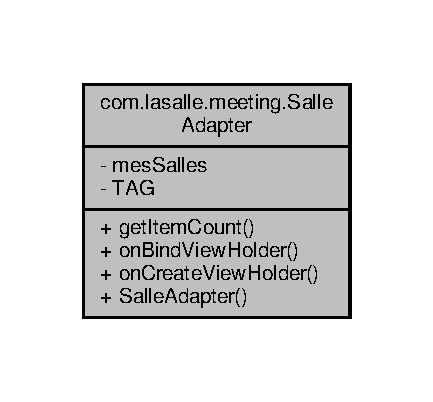
\includegraphics[width=208pt]{classcom_1_1lasalle_1_1meeting_1_1_salle_adapter__coll__graph}
\end{center}
\end{figure}
\subsubsection*{Fonctions membres publiques}
\begin{DoxyCompactItemize}
\item 
int \hyperlink{classcom_1_1lasalle_1_1meeting_1_1_salle_adapter_a4ee9f3c4b020c3bfd88e072bb21bc5fc}{get\+Item\+Count} ()
\begin{DoxyCompactList}\small\item\em Méthode appelée à la création de l\textquotesingle{}activité \hyperlink{classcom_1_1lasalle_1_1meeting_1_1_salle_adapter}{Salle\+Adapter}. \end{DoxyCompactList}\item 
void \hyperlink{classcom_1_1lasalle_1_1meeting_1_1_salle_adapter_ac196b478a0ea01a05455bfe15111406f}{on\+Bind\+View\+Holder} (@Non\+Null \hyperlink{classcom_1_1lasalle_1_1meeting_1_1_salle_view_holder}{Salle\+View\+Holder} holder, int position)
\begin{DoxyCompactList}\small\item\em Méthode appelée à la création de l\textquotesingle{}activité \hyperlink{classcom_1_1lasalle_1_1meeting_1_1_salle_adapter}{Salle\+Adapter}. \end{DoxyCompactList}\item 
\hyperlink{classcom_1_1lasalle_1_1meeting_1_1_salle_view_holder}{Salle\+View\+Holder} \hyperlink{classcom_1_1lasalle_1_1meeting_1_1_salle_adapter_a35aef67b6f83b63fdc9898f6024b24ac}{on\+Create\+View\+Holder} (@Non\+Null View\+Group parent, int view\+Type)
\begin{DoxyCompactList}\small\item\em Méthode appelée à la création de l\textquotesingle{}activité \hyperlink{classcom_1_1lasalle_1_1meeting_1_1_salle_adapter}{Salle\+Adapter}. \end{DoxyCompactList}\item 
\hyperlink{classcom_1_1lasalle_1_1meeting_1_1_salle_adapter_aac5caf27dc7448e1f37868066b3c9d00}{Salle\+Adapter} (Vector$<$ \hyperlink{classcom_1_1lasalle_1_1meeting_1_1_salle}{Salle} $>$ \hyperlink{classcom_1_1lasalle_1_1meeting_1_1_salle_adapter_a3988ff211fbf3052b553d77ba0711a5a}{mes\+Salles})
\begin{DoxyCompactList}\small\item\em constructeur de \hyperlink{classcom_1_1lasalle_1_1meeting_1_1_salle_adapter}{Salle\+Adapter} \end{DoxyCompactList}\end{DoxyCompactItemize}
\subsubsection*{Attributs privés}
\begin{DoxyCompactItemize}
\item 
Vector$<$ \hyperlink{classcom_1_1lasalle_1_1meeting_1_1_salle}{Salle} $>$ \hyperlink{classcom_1_1lasalle_1_1meeting_1_1_salle_adapter_a3988ff211fbf3052b553d77ba0711a5a}{mes\+Salles} = null
\begin{DoxyCompactList}\small\item\em Vecteur contenant mes salles. \end{DoxyCompactList}\end{DoxyCompactItemize}
\subsubsection*{Attributs privés statiques}
\begin{DoxyCompactItemize}
\item 
static final String \hyperlink{classcom_1_1lasalle_1_1meeting_1_1_salle_adapter_a774947591a1beedaffd58989783206b1}{T\+AG} = \char`\"{}Salle\+Adapter\char`\"{}
\begin{DoxyCompactList}\small\item\em T\+AG utilisé pour les logs. \end{DoxyCompactList}\end{DoxyCompactItemize}


\subsubsection{Description détaillée}
Déclaration de la classe \hyperlink{classcom_1_1lasalle_1_1meeting_1_1_salle_adapter}{Salle\+Adapter}. 

Définition à la ligne \hyperlink{_salle_adapter_8java_source_l00023}{23} du fichier \hyperlink{_salle_adapter_8java_source}{Salle\+Adapter.\+java}.



\subsubsection{Documentation des constructeurs et destructeur}
\mbox{\Hypertarget{classcom_1_1lasalle_1_1meeting_1_1_salle_adapter_aac5caf27dc7448e1f37868066b3c9d00}\label{classcom_1_1lasalle_1_1meeting_1_1_salle_adapter_aac5caf27dc7448e1f37868066b3c9d00}} 
\index{com\+::lasalle\+::meeting\+::\+Salle\+Adapter@{com\+::lasalle\+::meeting\+::\+Salle\+Adapter}!Salle\+Adapter@{Salle\+Adapter}}
\index{Salle\+Adapter@{Salle\+Adapter}!com\+::lasalle\+::meeting\+::\+Salle\+Adapter@{com\+::lasalle\+::meeting\+::\+Salle\+Adapter}}
\paragraph{\texorpdfstring{Salle\+Adapter()}{SalleAdapter()}}
{\footnotesize\ttfamily com.\+lasalle.\+meeting.\+Salle\+Adapter.\+Salle\+Adapter (\begin{DoxyParamCaption}\item[{Vector$<$ \hyperlink{classcom_1_1lasalle_1_1meeting_1_1_salle}{Salle} $>$}]{mes\+Salles }\end{DoxyParamCaption})}



constructeur de \hyperlink{classcom_1_1lasalle_1_1meeting_1_1_salle_adapter}{Salle\+Adapter} 


\begin{DoxyParams}{Paramètres}
{\em mes\+Salles} & Vector$<$\+Salle$>$ \\
\hline
\end{DoxyParams}


Définition à la ligne \hyperlink{_salle_adapter_8java_source_l00038}{38} du fichier \hyperlink{_salle_adapter_8java_source}{Salle\+Adapter.\+java}.



Références \hyperlink{_salle_adapter_8java_source_l00032}{com.\+lasalle.\+meeting.\+Salle\+Adapter.\+mes\+Salles}.


\begin{DoxyCode}
00039     \{
00040         Log.d(\hyperlink{classcom_1_1lasalle_1_1meeting_1_1_salle_adapter_a774947591a1beedaffd58989783206b1}{TAG}, \textcolor{stringliteral}{"SalleAdapter (Vector<Salle>)"});
00041 
00042         \textcolor{keywordflow}{if} (\hyperlink{classcom_1_1lasalle_1_1meeting_1_1_salle_adapter_a3988ff211fbf3052b553d77ba0711a5a}{mesSalles} != null) \{
00043             this.\hyperlink{classcom_1_1lasalle_1_1meeting_1_1_salle_adapter_a3988ff211fbf3052b553d77ba0711a5a}{mesSalles} = \hyperlink{classcom_1_1lasalle_1_1meeting_1_1_salle_adapter_a3988ff211fbf3052b553d77ba0711a5a}{mesSalles};
00044         \}
00045     \}
\end{DoxyCode}


\subsubsection{Documentation des fonctions membres}
\mbox{\Hypertarget{classcom_1_1lasalle_1_1meeting_1_1_salle_adapter_a4ee9f3c4b020c3bfd88e072bb21bc5fc}\label{classcom_1_1lasalle_1_1meeting_1_1_salle_adapter_a4ee9f3c4b020c3bfd88e072bb21bc5fc}} 
\index{com\+::lasalle\+::meeting\+::\+Salle\+Adapter@{com\+::lasalle\+::meeting\+::\+Salle\+Adapter}!get\+Item\+Count@{get\+Item\+Count}}
\index{get\+Item\+Count@{get\+Item\+Count}!com\+::lasalle\+::meeting\+::\+Salle\+Adapter@{com\+::lasalle\+::meeting\+::\+Salle\+Adapter}}
\paragraph{\texorpdfstring{get\+Item\+Count()}{getItemCount()}}
{\footnotesize\ttfamily int com.\+lasalle.\+meeting.\+Salle\+Adapter.\+get\+Item\+Count (\begin{DoxyParamCaption}{ }\end{DoxyParamCaption})}



Méthode appelée à la création de l\textquotesingle{}activité \hyperlink{classcom_1_1lasalle_1_1meeting_1_1_salle_adapter}{Salle\+Adapter}. 

\begin{DoxyReturn}{Renvoie}
int 
\end{DoxyReturn}


Définition à la ligne \hyperlink{_salle_adapter_8java_source_l00080}{80} du fichier \hyperlink{_salle_adapter_8java_source}{Salle\+Adapter.\+java}.


\begin{DoxyCode}
00080                               \{
00081         Log.d(\hyperlink{classcom_1_1lasalle_1_1meeting_1_1_salle_adapter_a774947591a1beedaffd58989783206b1}{TAG}, \textcolor{stringliteral}{"getItemCount()"});
00082         \textcolor{keywordflow}{if} (\hyperlink{classcom_1_1lasalle_1_1meeting_1_1_salle_adapter_a3988ff211fbf3052b553d77ba0711a5a}{mesSalles} != null)
00083             \textcolor{keywordflow}{return} \hyperlink{classcom_1_1lasalle_1_1meeting_1_1_salle_adapter_a3988ff211fbf3052b553d77ba0711a5a}{mesSalles}.size();
00084         \textcolor{keywordflow}{return} 0;
00085     \}
\end{DoxyCode}
\mbox{\Hypertarget{classcom_1_1lasalle_1_1meeting_1_1_salle_adapter_ac196b478a0ea01a05455bfe15111406f}\label{classcom_1_1lasalle_1_1meeting_1_1_salle_adapter_ac196b478a0ea01a05455bfe15111406f}} 
\index{com\+::lasalle\+::meeting\+::\+Salle\+Adapter@{com\+::lasalle\+::meeting\+::\+Salle\+Adapter}!on\+Bind\+View\+Holder@{on\+Bind\+View\+Holder}}
\index{on\+Bind\+View\+Holder@{on\+Bind\+View\+Holder}!com\+::lasalle\+::meeting\+::\+Salle\+Adapter@{com\+::lasalle\+::meeting\+::\+Salle\+Adapter}}
\paragraph{\texorpdfstring{on\+Bind\+View\+Holder()}{onBindViewHolder()}}
{\footnotesize\ttfamily void com.\+lasalle.\+meeting.\+Salle\+Adapter.\+on\+Bind\+View\+Holder (\begin{DoxyParamCaption}\item[{@Non\+Null \hyperlink{classcom_1_1lasalle_1_1meeting_1_1_salle_view_holder}{Salle\+View\+Holder}}]{holder,  }\item[{int}]{position }\end{DoxyParamCaption})}



Méthode appelée à la création de l\textquotesingle{}activité \hyperlink{classcom_1_1lasalle_1_1meeting_1_1_salle_adapter}{Salle\+Adapter}. 


\begin{DoxyParams}{Paramètres}
{\em holder} & \hyperlink{classcom_1_1lasalle_1_1meeting_1_1_salle_view_holder}{Salle\+View\+Holder}, position int \\
\hline
\end{DoxyParams}
\begin{DoxyReturn}{Renvoie}
void 
\end{DoxyReturn}


Définition à la ligne \hyperlink{_salle_adapter_8java_source_l00068}{68} du fichier \hyperlink{_salle_adapter_8java_source}{Salle\+Adapter.\+java}.


\begin{DoxyCode}
00069     \{
00070         Log.d(\hyperlink{classcom_1_1lasalle_1_1meeting_1_1_salle_adapter_a774947591a1beedaffd58989783206b1}{TAG}, \textcolor{stringliteral}{"onBindViewHolder()"});
00071         Salle salle = \hyperlink{classcom_1_1lasalle_1_1meeting_1_1_salle_adapter_a3988ff211fbf3052b553d77ba0711a5a}{mesSalles}.get(position);
00072         holder.afficher(salle);
00073     \}
\end{DoxyCode}
\mbox{\Hypertarget{classcom_1_1lasalle_1_1meeting_1_1_salle_adapter_a35aef67b6f83b63fdc9898f6024b24ac}\label{classcom_1_1lasalle_1_1meeting_1_1_salle_adapter_a35aef67b6f83b63fdc9898f6024b24ac}} 
\index{com\+::lasalle\+::meeting\+::\+Salle\+Adapter@{com\+::lasalle\+::meeting\+::\+Salle\+Adapter}!on\+Create\+View\+Holder@{on\+Create\+View\+Holder}}
\index{on\+Create\+View\+Holder@{on\+Create\+View\+Holder}!com\+::lasalle\+::meeting\+::\+Salle\+Adapter@{com\+::lasalle\+::meeting\+::\+Salle\+Adapter}}
\paragraph{\texorpdfstring{on\+Create\+View\+Holder()}{onCreateViewHolder()}}
{\footnotesize\ttfamily \hyperlink{classcom_1_1lasalle_1_1meeting_1_1_salle_view_holder}{Salle\+View\+Holder} com.\+lasalle.\+meeting.\+Salle\+Adapter.\+on\+Create\+View\+Holder (\begin{DoxyParamCaption}\item[{@Non\+Null View\+Group}]{parent,  }\item[{int}]{view\+Type }\end{DoxyParamCaption})}



Méthode appelée à la création de l\textquotesingle{}activité \hyperlink{classcom_1_1lasalle_1_1meeting_1_1_salle_adapter}{Salle\+Adapter}. 


\begin{DoxyParams}{Paramètres}
{\em parent} & View\+Group, view\+Type int \\
\hline
\end{DoxyParams}
\begin{DoxyReturn}{Renvoie}
\hyperlink{classcom_1_1lasalle_1_1meeting_1_1_salle_view_holder}{Salle\+View\+Holder} 
\end{DoxyReturn}


Définition à la ligne \hyperlink{_salle_adapter_8java_source_l00054}{54} du fichier \hyperlink{_salle_adapter_8java_source}{Salle\+Adapter.\+java}.


\begin{DoxyCode}
00055     \{
00056         Log.d(\hyperlink{classcom_1_1lasalle_1_1meeting_1_1_salle_adapter_a774947591a1beedaffd58989783206b1}{TAG}, \textcolor{stringliteral}{"SalleViewHolder onCreateViewHolder()"});
00057         LayoutInflater inflater = LayoutInflater.from(parent.getContext());
00058         View view = inflater.inflate(R.layout.salle, parent, \textcolor{keyword}{false});
00059         \textcolor{keywordflow}{return} \textcolor{keyword}{new} SalleViewHolder(view);
00060     \}
\end{DoxyCode}


\subsubsection{Documentation des données membres}
\mbox{\Hypertarget{classcom_1_1lasalle_1_1meeting_1_1_salle_adapter_a3988ff211fbf3052b553d77ba0711a5a}\label{classcom_1_1lasalle_1_1meeting_1_1_salle_adapter_a3988ff211fbf3052b553d77ba0711a5a}} 
\index{com\+::lasalle\+::meeting\+::\+Salle\+Adapter@{com\+::lasalle\+::meeting\+::\+Salle\+Adapter}!mes\+Salles@{mes\+Salles}}
\index{mes\+Salles@{mes\+Salles}!com\+::lasalle\+::meeting\+::\+Salle\+Adapter@{com\+::lasalle\+::meeting\+::\+Salle\+Adapter}}
\paragraph{\texorpdfstring{mes\+Salles}{mesSalles}}
{\footnotesize\ttfamily Vector$<$\hyperlink{classcom_1_1lasalle_1_1meeting_1_1_salle}{Salle}$>$ com.\+lasalle.\+meeting.\+Salle\+Adapter.\+mes\+Salles = null\hspace{0.3cm}{\ttfamily [private]}}



Vecteur contenant mes salles. 

Attributs 

Définition à la ligne \hyperlink{_salle_adapter_8java_source_l00032}{32} du fichier \hyperlink{_salle_adapter_8java_source}{Salle\+Adapter.\+java}.



Référencé par \hyperlink{_salle_adapter_8java_source_l00038}{com.\+lasalle.\+meeting.\+Salle\+Adapter.\+Salle\+Adapter()}.

\mbox{\Hypertarget{classcom_1_1lasalle_1_1meeting_1_1_salle_adapter_a774947591a1beedaffd58989783206b1}\label{classcom_1_1lasalle_1_1meeting_1_1_salle_adapter_a774947591a1beedaffd58989783206b1}} 
\index{com\+::lasalle\+::meeting\+::\+Salle\+Adapter@{com\+::lasalle\+::meeting\+::\+Salle\+Adapter}!T\+AG@{T\+AG}}
\index{T\+AG@{T\+AG}!com\+::lasalle\+::meeting\+::\+Salle\+Adapter@{com\+::lasalle\+::meeting\+::\+Salle\+Adapter}}
\paragraph{\texorpdfstring{T\+AG}{TAG}}
{\footnotesize\ttfamily final String com.\+lasalle.\+meeting.\+Salle\+Adapter.\+T\+AG = \char`\"{}Salle\+Adapter\char`\"{}\hspace{0.3cm}{\ttfamily [static]}, {\ttfamily [private]}}



T\+AG utilisé pour les logs. 

Constantes 

Définition à la ligne \hyperlink{_salle_adapter_8java_source_l00028}{28} du fichier \hyperlink{_salle_adapter_8java_source}{Salle\+Adapter.\+java}.



La documentation de cette classe a été générée à partir du fichier suivant \+:\begin{DoxyCompactItemize}
\item 
\hyperlink{_salle_adapter_8java}{Salle\+Adapter.\+java}\end{DoxyCompactItemize}

\hypertarget{classcom_1_1lasalle_1_1meeting_1_1_salle_view_holder}{}\subsection{Référence de la classe com.\+lasalle.\+meeting.\+Salle\+View\+Holder}
\label{classcom_1_1lasalle_1_1meeting_1_1_salle_view_holder}\index{com.\+lasalle.\+meeting.\+Salle\+View\+Holder@{com.\+lasalle.\+meeting.\+Salle\+View\+Holder}}


Déclaration de la classe \hyperlink{classcom_1_1lasalle_1_1meeting_1_1_salle_view_holder}{Salle\+View\+Holder}.  




Graphe de collaboration de com.\+lasalle.\+meeting.\+Salle\+View\+Holder\+:
\nopagebreak
\begin{figure}[H]
\begin{center}
\leavevmode
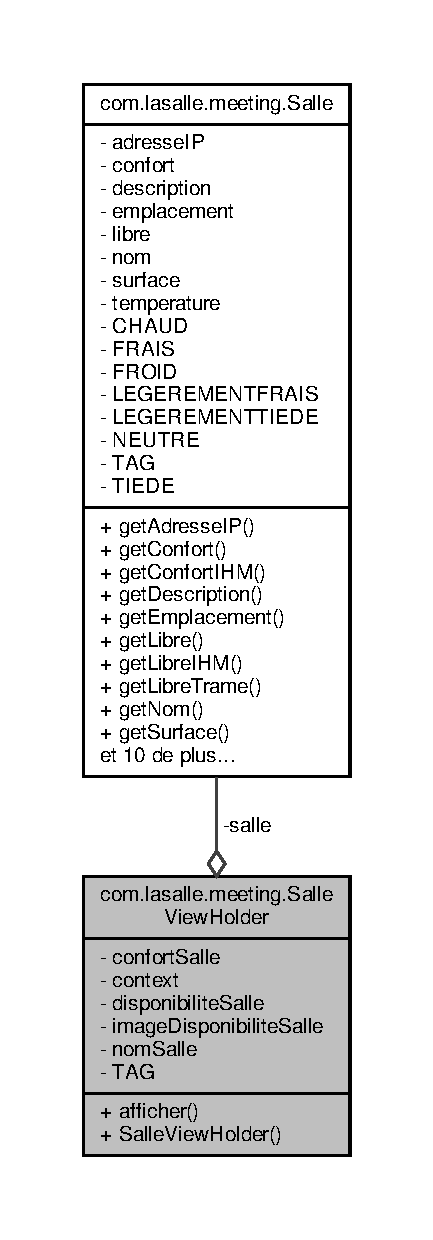
\includegraphics[height=550pt]{classcom_1_1lasalle_1_1meeting_1_1_salle_view_holder__coll__graph}
\end{center}
\end{figure}
\subsubsection*{Fonctions membres publiques}
\begin{DoxyCompactItemize}
\item 
void \hyperlink{classcom_1_1lasalle_1_1meeting_1_1_salle_view_holder_ac9f5e4bd25c8abc50ad524e0c2132304}{afficher} (\hyperlink{classcom_1_1lasalle_1_1meeting_1_1_salle}{Salle} \hyperlink{classcom_1_1lasalle_1_1meeting_1_1_salle_view_holder_afe85265c9d35c5035e96ace9c8032606}{salle})
\begin{DoxyCompactList}\small\item\em Méthode affichant les informations de la salle dans les layouts. \end{DoxyCompactList}\item 
\hyperlink{classcom_1_1lasalle_1_1meeting_1_1_salle_view_holder_ab123df6edb081221dc36daff6f8c1763}{Salle\+View\+Holder} (final View item\+View)
\begin{DoxyCompactList}\small\item\em constructeur de \hyperlink{classcom_1_1lasalle_1_1meeting_1_1_salle_view_holder}{Salle\+View\+Holder} \end{DoxyCompactList}\end{DoxyCompactItemize}
\subsubsection*{Attributs privés}
\begin{DoxyCompactItemize}
\item 
Text\+View \hyperlink{classcom_1_1lasalle_1_1meeting_1_1_salle_view_holder_adb1ed56224bf4c72f3b6ceadd1e20da5}{confort\+Salle}
\begin{DoxyCompactList}\small\item\em layout texte du confort de la salle \end{DoxyCompactList}\item 
Context \hyperlink{classcom_1_1lasalle_1_1meeting_1_1_salle_view_holder_a7072e3d124129f260af7a24c7ad4277d}{context}
\begin{DoxyCompactList}\small\item\em attribut permettant de communiquer avec une autre classe \end{DoxyCompactList}\item 
Text\+View \hyperlink{classcom_1_1lasalle_1_1meeting_1_1_salle_view_holder_a022ce4875ad260fe538779ae45fae90a}{disponibilite\+Salle}
\begin{DoxyCompactList}\small\item\em layout texte de la disponibilité de la salle \end{DoxyCompactList}\item 
Image\+View \hyperlink{classcom_1_1lasalle_1_1meeting_1_1_salle_view_holder_aa062c074e992faadf2386744ea33034f}{image\+Disponibilite\+Salle}
\begin{DoxyCompactList}\small\item\em layout image de la disponibilité de la salle \end{DoxyCompactList}\item 
Text\+View \hyperlink{classcom_1_1lasalle_1_1meeting_1_1_salle_view_holder_a54d26a89113e63e36c17c4ed9253f058}{nom\+Salle}
\begin{DoxyCompactList}\small\item\em layout texte du nom de la salle \end{DoxyCompactList}\item 
\hyperlink{classcom_1_1lasalle_1_1meeting_1_1_salle}{Salle} \hyperlink{classcom_1_1lasalle_1_1meeting_1_1_salle_view_holder_afe85265c9d35c5035e96ace9c8032606}{salle}
\begin{DoxyCompactList}\small\item\em attribut salle \end{DoxyCompactList}\end{DoxyCompactItemize}
\subsubsection*{Attributs privés statiques}
\begin{DoxyCompactItemize}
\item 
static final String \hyperlink{classcom_1_1lasalle_1_1meeting_1_1_salle_view_holder_acde5b16df12d2d83074c53bbfe7220b9}{T\+AG} = \char`\"{}Salle\+View\+Holder\char`\"{}
\begin{DoxyCompactList}\small\item\em T\+AG utilisé pour les logs. \end{DoxyCompactList}\end{DoxyCompactItemize}


\subsubsection{Description détaillée}
Déclaration de la classe \hyperlink{classcom_1_1lasalle_1_1meeting_1_1_salle_view_holder}{Salle\+View\+Holder}. 

Définition à la ligne \hyperlink{_salle_view_holder_8java_source_l00025}{25} du fichier \hyperlink{_salle_view_holder_8java_source}{Salle\+View\+Holder.\+java}.



\subsubsection{Documentation des constructeurs et destructeur}
\mbox{\Hypertarget{classcom_1_1lasalle_1_1meeting_1_1_salle_view_holder_ab123df6edb081221dc36daff6f8c1763}\label{classcom_1_1lasalle_1_1meeting_1_1_salle_view_holder_ab123df6edb081221dc36daff6f8c1763}} 
\index{com\+::lasalle\+::meeting\+::\+Salle\+View\+Holder@{com\+::lasalle\+::meeting\+::\+Salle\+View\+Holder}!Salle\+View\+Holder@{Salle\+View\+Holder}}
\index{Salle\+View\+Holder@{Salle\+View\+Holder}!com\+::lasalle\+::meeting\+::\+Salle\+View\+Holder@{com\+::lasalle\+::meeting\+::\+Salle\+View\+Holder}}
\paragraph{\texorpdfstring{Salle\+View\+Holder()}{SalleViewHolder()}}
{\footnotesize\ttfamily com.\+lasalle.\+meeting.\+Salle\+View\+Holder.\+Salle\+View\+Holder (\begin{DoxyParamCaption}\item[{final View}]{item\+View }\end{DoxyParamCaption})}



constructeur de \hyperlink{classcom_1_1lasalle_1_1meeting_1_1_salle_view_holder}{Salle\+View\+Holder} 


\begin{DoxyParams}{Paramètres}
{\em item\+View} & final View \\
\hline
\end{DoxyParams}


Définition à la ligne \hyperlink{_salle_view_holder_8java_source_l00049}{49} du fichier \hyperlink{_salle_view_holder_8java_source}{Salle\+View\+Holder.\+java}.


\begin{DoxyCode}
00050     \{
00051         super(itemView);
00052 
00053         Log.d(\hyperlink{classcom_1_1lasalle_1_1meeting_1_1_salle_view_holder_acde5b16df12d2d83074c53bbfe7220b9}{TAG}, \textcolor{stringliteral}{"SalleViewHolder(final View itemView)"});
00054 
00055         \hyperlink{classcom_1_1lasalle_1_1meeting_1_1_salle_view_holder_a54d26a89113e63e36c17c4ed9253f058}{nomSalle}= ((TextView)itemView.findViewById(R.id.nomSalle));
00056         \hyperlink{classcom_1_1lasalle_1_1meeting_1_1_salle_view_holder_adb1ed56224bf4c72f3b6ceadd1e20da5}{confortSalle} = ((TextView)itemView.findViewById(R.id.confortSalle));
00057         \hyperlink{classcom_1_1lasalle_1_1meeting_1_1_salle_view_holder_a022ce4875ad260fe538779ae45fae90a}{disponibiliteSalle} = ((TextView)itemView.findViewById(R.id.disponibiliteSalle));
00058         \hyperlink{classcom_1_1lasalle_1_1meeting_1_1_salle_view_holder_aa062c074e992faadf2386744ea33034f}{imageDisponibiliteSalle} = ((ImageView)itemView.findViewById(R.id.
      imageDisponibiliteSalle));
00059         \hyperlink{classcom_1_1lasalle_1_1meeting_1_1_salle_view_holder_a7072e3d124129f260af7a24c7ad4277d}{context} = itemView.getContext();
00060 
00061         itemView.setOnClickListener(\textcolor{keyword}{new} View.OnClickListener()
00062         \{
00063             @Override
00064             \textcolor{keyword}{public} \textcolor{keywordtype}{void} onClick(View view)
00065             \{
00066                 Intent intent = \textcolor{keyword}{new} Intent(\hyperlink{classcom_1_1lasalle_1_1meeting_1_1_salle_view_holder_a7072e3d124129f260af7a24c7ad4277d}{context}, SalleActivity.class);
00067                 intent.putExtra(\textcolor{stringliteral}{"Salle"}, (Serializable) \hyperlink{classcom_1_1lasalle_1_1meeting_1_1_salle_view_holder_afe85265c9d35c5035e96ace9c8032606}{salle});
00068                 \hyperlink{classcom_1_1lasalle_1_1meeting_1_1_salle_view_holder_a7072e3d124129f260af7a24c7ad4277d}{context}.startActivity(intent);
00069             \}
00070         \});
00071     \}
\end{DoxyCode}


\subsubsection{Documentation des fonctions membres}
\mbox{\Hypertarget{classcom_1_1lasalle_1_1meeting_1_1_salle_view_holder_ac9f5e4bd25c8abc50ad524e0c2132304}\label{classcom_1_1lasalle_1_1meeting_1_1_salle_view_holder_ac9f5e4bd25c8abc50ad524e0c2132304}} 
\index{com\+::lasalle\+::meeting\+::\+Salle\+View\+Holder@{com\+::lasalle\+::meeting\+::\+Salle\+View\+Holder}!afficher@{afficher}}
\index{afficher@{afficher}!com\+::lasalle\+::meeting\+::\+Salle\+View\+Holder@{com\+::lasalle\+::meeting\+::\+Salle\+View\+Holder}}
\paragraph{\texorpdfstring{afficher()}{afficher()}}
{\footnotesize\ttfamily void com.\+lasalle.\+meeting.\+Salle\+View\+Holder.\+afficher (\begin{DoxyParamCaption}\item[{\hyperlink{classcom_1_1lasalle_1_1meeting_1_1_salle}{Salle}}]{salle }\end{DoxyParamCaption})}



Méthode affichant les informations de la salle dans les layouts. 

\begin{DoxyReturn}{Renvoie}
void 
\end{DoxyReturn}


Définition à la ligne \hyperlink{_salle_view_holder_8java_source_l00077}{77} du fichier \hyperlink{_salle_view_holder_8java_source}{Salle\+View\+Holder.\+java}.



Références \hyperlink{_salle_8java_source_l00233}{com.\+lasalle.\+meeting.\+Salle.\+get\+Confort\+I\+H\+M()}, \hyperlink{_salle_8java_source_l00174}{com.\+lasalle.\+meeting.\+Salle.\+get\+Libre()}, \hyperlink{_salle_8java_source_l00199}{com.\+lasalle.\+meeting.\+Salle.\+get\+Libre\+I\+H\+M()}, \hyperlink{_salle_8java_source_l00165}{com.\+lasalle.\+meeting.\+Salle.\+get\+Nom()}, et \hyperlink{_salle_view_holder_8java_source_l00042}{com.\+lasalle.\+meeting.\+Salle\+View\+Holder.\+salle}.


\begin{DoxyCode}
00078     \{
00079         Log.d(\hyperlink{classcom_1_1lasalle_1_1meeting_1_1_salle_view_holder_acde5b16df12d2d83074c53bbfe7220b9}{TAG}, \textcolor{stringliteral}{"afficher ()"});
00080 
00081         this.\hyperlink{classcom_1_1lasalle_1_1meeting_1_1_salle_view_holder_afe85265c9d35c5035e96ace9c8032606}{salle}= \hyperlink{classcom_1_1lasalle_1_1meeting_1_1_salle_view_holder_afe85265c9d35c5035e96ace9c8032606}{salle};
00082         \hyperlink{classcom_1_1lasalle_1_1meeting_1_1_salle_view_holder_a54d26a89113e63e36c17c4ed9253f058}{nomSalle}.setText(\hyperlink{classcom_1_1lasalle_1_1meeting_1_1_salle_view_holder_afe85265c9d35c5035e96ace9c8032606}{salle}.\hyperlink{classcom_1_1lasalle_1_1meeting_1_1_salle_a49d977f69b2783e8ad57eccffc29e97b}{getNom}());
00083         \hyperlink{classcom_1_1lasalle_1_1meeting_1_1_salle_view_holder_a54d26a89113e63e36c17c4ed9253f058}{nomSalle}.setTextSize(15);
00084         \hyperlink{classcom_1_1lasalle_1_1meeting_1_1_salle_view_holder_adb1ed56224bf4c72f3b6ceadd1e20da5}{confortSalle}.setText(\hyperlink{classcom_1_1lasalle_1_1meeting_1_1_salle_view_holder_afe85265c9d35c5035e96ace9c8032606}{salle}.\hyperlink{classcom_1_1lasalle_1_1meeting_1_1_salle_abf1f96423a1df46ba4d6ac4a1b6d0c34}{getConfortIHM}());
00085         \hyperlink{classcom_1_1lasalle_1_1meeting_1_1_salle_view_holder_adb1ed56224bf4c72f3b6ceadd1e20da5}{confortSalle}.setTextSize(15);
00086         \hyperlink{classcom_1_1lasalle_1_1meeting_1_1_salle_view_holder_a022ce4875ad260fe538779ae45fae90a}{disponibiliteSalle}.setText(\textcolor{stringliteral}{"La salle est "}+ \hyperlink{classcom_1_1lasalle_1_1meeting_1_1_salle_view_holder_afe85265c9d35c5035e96ace9c8032606}{salle}.
      \hyperlink{classcom_1_1lasalle_1_1meeting_1_1_salle_ab86dfb73018e96230ceed49e207a8971}{getLibreIHM}());
00087         \hyperlink{classcom_1_1lasalle_1_1meeting_1_1_salle_view_holder_a022ce4875ad260fe538779ae45fae90a}{disponibiliteSalle}.setTextSize(15);
00088 
00089         \textcolor{keywordflow}{if}(\hyperlink{classcom_1_1lasalle_1_1meeting_1_1_salle_view_holder_afe85265c9d35c5035e96ace9c8032606}{salle}.\hyperlink{classcom_1_1lasalle_1_1meeting_1_1_salle_adc0c4936355bc0ae22991f69c12a5e42}{getLibre}())
00090         \{
00091             \hyperlink{classcom_1_1lasalle_1_1meeting_1_1_salle_view_holder_aa062c074e992faadf2386744ea33034f}{imageDisponibiliteSalle}.setImageResource(R.drawable.rond\_vert);
00092         \}
00093         \textcolor{keywordflow}{else}
00094         \{
00095             \hyperlink{classcom_1_1lasalle_1_1meeting_1_1_salle_view_holder_aa062c074e992faadf2386744ea33034f}{imageDisponibiliteSalle}.setImageResource(R.drawable.rond\_rouge);
00096         \}
00097     \}
\end{DoxyCode}


\subsubsection{Documentation des données membres}
\mbox{\Hypertarget{classcom_1_1lasalle_1_1meeting_1_1_salle_view_holder_adb1ed56224bf4c72f3b6ceadd1e20da5}\label{classcom_1_1lasalle_1_1meeting_1_1_salle_view_holder_adb1ed56224bf4c72f3b6ceadd1e20da5}} 
\index{com\+::lasalle\+::meeting\+::\+Salle\+View\+Holder@{com\+::lasalle\+::meeting\+::\+Salle\+View\+Holder}!confort\+Salle@{confort\+Salle}}
\index{confort\+Salle@{confort\+Salle}!com\+::lasalle\+::meeting\+::\+Salle\+View\+Holder@{com\+::lasalle\+::meeting\+::\+Salle\+View\+Holder}}
\paragraph{\texorpdfstring{confort\+Salle}{confortSalle}}
{\footnotesize\ttfamily Text\+View com.\+lasalle.\+meeting.\+Salle\+View\+Holder.\+confort\+Salle\hspace{0.3cm}{\ttfamily [private]}}



layout texte du confort de la salle 



Définition à la ligne \hyperlink{_salle_view_holder_8java_source_l00035}{35} du fichier \hyperlink{_salle_view_holder_8java_source}{Salle\+View\+Holder.\+java}.

\mbox{\Hypertarget{classcom_1_1lasalle_1_1meeting_1_1_salle_view_holder_a7072e3d124129f260af7a24c7ad4277d}\label{classcom_1_1lasalle_1_1meeting_1_1_salle_view_holder_a7072e3d124129f260af7a24c7ad4277d}} 
\index{com\+::lasalle\+::meeting\+::\+Salle\+View\+Holder@{com\+::lasalle\+::meeting\+::\+Salle\+View\+Holder}!context@{context}}
\index{context@{context}!com\+::lasalle\+::meeting\+::\+Salle\+View\+Holder@{com\+::lasalle\+::meeting\+::\+Salle\+View\+Holder}}
\paragraph{\texorpdfstring{context}{context}}
{\footnotesize\ttfamily Context com.\+lasalle.\+meeting.\+Salle\+View\+Holder.\+context\hspace{0.3cm}{\ttfamily [private]}}



attribut permettant de communiquer avec une autre classe 

Attributs 

Définition à la ligne \hyperlink{_salle_view_holder_8java_source_l00041}{41} du fichier \hyperlink{_salle_view_holder_8java_source}{Salle\+View\+Holder.\+java}.

\mbox{\Hypertarget{classcom_1_1lasalle_1_1meeting_1_1_salle_view_holder_a022ce4875ad260fe538779ae45fae90a}\label{classcom_1_1lasalle_1_1meeting_1_1_salle_view_holder_a022ce4875ad260fe538779ae45fae90a}} 
\index{com\+::lasalle\+::meeting\+::\+Salle\+View\+Holder@{com\+::lasalle\+::meeting\+::\+Salle\+View\+Holder}!disponibilite\+Salle@{disponibilite\+Salle}}
\index{disponibilite\+Salle@{disponibilite\+Salle}!com\+::lasalle\+::meeting\+::\+Salle\+View\+Holder@{com\+::lasalle\+::meeting\+::\+Salle\+View\+Holder}}
\paragraph{\texorpdfstring{disponibilite\+Salle}{disponibiliteSalle}}
{\footnotesize\ttfamily Text\+View com.\+lasalle.\+meeting.\+Salle\+View\+Holder.\+disponibilite\+Salle\hspace{0.3cm}{\ttfamily [private]}}



layout texte de la disponibilité de la salle 



Définition à la ligne \hyperlink{_salle_view_holder_8java_source_l00036}{36} du fichier \hyperlink{_salle_view_holder_8java_source}{Salle\+View\+Holder.\+java}.

\mbox{\Hypertarget{classcom_1_1lasalle_1_1meeting_1_1_salle_view_holder_aa062c074e992faadf2386744ea33034f}\label{classcom_1_1lasalle_1_1meeting_1_1_salle_view_holder_aa062c074e992faadf2386744ea33034f}} 
\index{com\+::lasalle\+::meeting\+::\+Salle\+View\+Holder@{com\+::lasalle\+::meeting\+::\+Salle\+View\+Holder}!image\+Disponibilite\+Salle@{image\+Disponibilite\+Salle}}
\index{image\+Disponibilite\+Salle@{image\+Disponibilite\+Salle}!com\+::lasalle\+::meeting\+::\+Salle\+View\+Holder@{com\+::lasalle\+::meeting\+::\+Salle\+View\+Holder}}
\paragraph{\texorpdfstring{image\+Disponibilite\+Salle}{imageDisponibiliteSalle}}
{\footnotesize\ttfamily Image\+View com.\+lasalle.\+meeting.\+Salle\+View\+Holder.\+image\+Disponibilite\+Salle\hspace{0.3cm}{\ttfamily [private]}}



layout image de la disponibilité de la salle 



Définition à la ligne \hyperlink{_salle_view_holder_8java_source_l00037}{37} du fichier \hyperlink{_salle_view_holder_8java_source}{Salle\+View\+Holder.\+java}.

\mbox{\Hypertarget{classcom_1_1lasalle_1_1meeting_1_1_salle_view_holder_a54d26a89113e63e36c17c4ed9253f058}\label{classcom_1_1lasalle_1_1meeting_1_1_salle_view_holder_a54d26a89113e63e36c17c4ed9253f058}} 
\index{com\+::lasalle\+::meeting\+::\+Salle\+View\+Holder@{com\+::lasalle\+::meeting\+::\+Salle\+View\+Holder}!nom\+Salle@{nom\+Salle}}
\index{nom\+Salle@{nom\+Salle}!com\+::lasalle\+::meeting\+::\+Salle\+View\+Holder@{com\+::lasalle\+::meeting\+::\+Salle\+View\+Holder}}
\paragraph{\texorpdfstring{nom\+Salle}{nomSalle}}
{\footnotesize\ttfamily Text\+View com.\+lasalle.\+meeting.\+Salle\+View\+Holder.\+nom\+Salle\hspace{0.3cm}{\ttfamily [private]}}



layout texte du nom de la salle 

Ressources layout activity\+\_\+main 

Définition à la ligne \hyperlink{_salle_view_holder_8java_source_l00034}{34} du fichier \hyperlink{_salle_view_holder_8java_source}{Salle\+View\+Holder.\+java}.

\mbox{\Hypertarget{classcom_1_1lasalle_1_1meeting_1_1_salle_view_holder_afe85265c9d35c5035e96ace9c8032606}\label{classcom_1_1lasalle_1_1meeting_1_1_salle_view_holder_afe85265c9d35c5035e96ace9c8032606}} 
\index{com\+::lasalle\+::meeting\+::\+Salle\+View\+Holder@{com\+::lasalle\+::meeting\+::\+Salle\+View\+Holder}!salle@{salle}}
\index{salle@{salle}!com\+::lasalle\+::meeting\+::\+Salle\+View\+Holder@{com\+::lasalle\+::meeting\+::\+Salle\+View\+Holder}}
\paragraph{\texorpdfstring{salle}{salle}}
{\footnotesize\ttfamily \hyperlink{classcom_1_1lasalle_1_1meeting_1_1_salle}{Salle} com.\+lasalle.\+meeting.\+Salle\+View\+Holder.\+salle\hspace{0.3cm}{\ttfamily [private]}}



attribut salle 



Définition à la ligne \hyperlink{_salle_view_holder_8java_source_l00042}{42} du fichier \hyperlink{_salle_view_holder_8java_source}{Salle\+View\+Holder.\+java}.



Référencé par \hyperlink{_salle_view_holder_8java_source_l00077}{com.\+lasalle.\+meeting.\+Salle\+View\+Holder.\+afficher()}.

\mbox{\Hypertarget{classcom_1_1lasalle_1_1meeting_1_1_salle_view_holder_acde5b16df12d2d83074c53bbfe7220b9}\label{classcom_1_1lasalle_1_1meeting_1_1_salle_view_holder_acde5b16df12d2d83074c53bbfe7220b9}} 
\index{com\+::lasalle\+::meeting\+::\+Salle\+View\+Holder@{com\+::lasalle\+::meeting\+::\+Salle\+View\+Holder}!T\+AG@{T\+AG}}
\index{T\+AG@{T\+AG}!com\+::lasalle\+::meeting\+::\+Salle\+View\+Holder@{com\+::lasalle\+::meeting\+::\+Salle\+View\+Holder}}
\paragraph{\texorpdfstring{T\+AG}{TAG}}
{\footnotesize\ttfamily final String com.\+lasalle.\+meeting.\+Salle\+View\+Holder.\+T\+AG = \char`\"{}Salle\+View\+Holder\char`\"{}\hspace{0.3cm}{\ttfamily [static]}, {\ttfamily [private]}}



T\+AG utilisé pour les logs. 

Constantes 

Définition à la ligne \hyperlink{_salle_view_holder_8java_source_l00030}{30} du fichier \hyperlink{_salle_view_holder_8java_source}{Salle\+View\+Holder.\+java}.



La documentation de cette classe a été générée à partir du fichier suivant \+:\begin{DoxyCompactItemize}
\item 
\hyperlink{_salle_view_holder_8java}{Salle\+View\+Holder.\+java}\end{DoxyCompactItemize}

\section{Documentation des fichiers}
\hypertarget{_changelog_8md}{}\subsection{Référence du fichier Changelog.\+md}
\label{_changelog_8md}\index{Changelog.\+md@{Changelog.\+md}}

\hypertarget{_changelog_8md_source}{}\subsection{Changelog.\+md}

\begin{DoxyCode}
00001 \(\backslash\)page page\_changelog Changelog
00002 
00003 r1 | www-data | 2020-02-01 15:03:29 +0100 (sam. 01 févr. 2020) | 1 ligne
00004 
00005 Creating initial repository structure
\end{DoxyCode}

\hypertarget{_communication_8java}{}\subsection{Référence du fichier Communication.\+java}
\label{_communication_8java}\index{Communication.\+java@{Communication.\+java}}


Déclaration de la classe Communication.  


\subsubsection*{Classes}
\begin{DoxyCompactItemize}
\item 
class \hyperlink{classcom_1_1lasalle_1_1meeting_1_1_communication}{com.\+lasalle.\+meeting.\+Communication}
\begin{DoxyCompactList}\small\item\em Déclaration de la classe \hyperlink{classcom_1_1lasalle_1_1meeting_1_1_communication}{Communication}. \end{DoxyCompactList}\end{DoxyCompactItemize}
\subsubsection*{Paquetages}
\begin{DoxyCompactItemize}
\item 
package \hyperlink{namespacecom_1_1lasalle_1_1meeting}{com.\+lasalle.\+meeting}
\end{DoxyCompactItemize}


\subsubsection{Description détaillée}
Déclaration de la classe Communication. 

\begin{DoxyAuthor}{Auteur}
Vincent D\+E\+V\+I\+NE 
\end{DoxyAuthor}


Définition dans le fichier \hyperlink{_communication_8java_source}{Communication.\+java}.


\hypertarget{_communication_8java_source}{}\subsection{Communication.\+java}
\label{_communication_8java_source}\index{Communication.\+java@{Communication.\+java}}

\begin{DoxyCode}
\Hypertarget{_communication_8java_source_l00001}\hyperlink{namespacecom_1_1lasalle_1_1meeting}{00001} \textcolor{keyword}{package }com.lasalle.meeting;
00002 
00003 \textcolor{keyword}{import} android.os.Bundle;
00004 \textcolor{keyword}{import} android.os.Handler;
00005 \textcolor{keyword}{import} android.os.Message;
00006 \textcolor{keyword}{import} android.util.Log;
00007 \textcolor{keyword}{import} java.net.*;
00008 \textcolor{keyword}{import} java.io.IOException;
00009 \textcolor{keyword}{import} java.net.DatagramPacket;
00010 \textcolor{keyword}{import} java.net.Socket;
00011 \textcolor{keyword}{import} java.util.concurrent.locks.ReentrantLock;
00012 
\Hypertarget{_communication_8java_source_l00023}\hyperlink{classcom_1_1lasalle_1_1meeting_1_1_communication}{00023} \textcolor{keyword}{public} \textcolor{keyword}{class }\hyperlink{classcom_1_1lasalle_1_1meeting_1_1_communication}{Communication} \textcolor{keyword}{implements} \hyperlink{class_runnable}{Runnable}
00024 \{
\Hypertarget{_communication_8java_source_l00028}\hyperlink{classcom_1_1lasalle_1_1meeting_1_1_communication_a5d58f88df1f20b4d61edbed9a82eccab}{00028}     \textcolor{keyword}{private} \textcolor{keyword}{final} \textcolor{keyword}{static} String \hyperlink{classcom_1_1lasalle_1_1meeting_1_1_communication_a5d58f88df1f20b4d61edbed9a82eccab}{TAG} = \textcolor{stringliteral}{"Communication"};              
\Hypertarget{_communication_8java_source_l00029}\hyperlink{classcom_1_1lasalle_1_1meeting_1_1_communication_a6a2d2e62f87bef261a1999eb5acf8abb}{00029}     \textcolor{keyword}{private} \textcolor{keyword}{final} \textcolor{keyword}{static} String \hyperlink{classcom_1_1lasalle_1_1meeting_1_1_communication_a6a2d2e62f87bef261a1999eb5acf8abb}{adresseMulticast} = \textcolor{stringliteral}{"239.0.0.42"};    
\Hypertarget{_communication_8java_source_l00030}\hyperlink{classcom_1_1lasalle_1_1meeting_1_1_communication_abf48fd6a29d87d67f4941494404f1ea7}{00030}     \textcolor{keyword}{private} \textcolor{keyword}{final} \textcolor{keyword}{static} \textcolor{keywordtype}{int} \hyperlink{classcom_1_1lasalle_1_1meeting_1_1_communication_abf48fd6a29d87d67f4941494404f1ea7}{PORT} = 5000;                           
\Hypertarget{_communication_8java_source_l00031}\hyperlink{classcom_1_1lasalle_1_1meeting_1_1_communication_a7cbfa2bdd8c4978f96abd43740050fe0}{00031}     \textcolor{keyword}{public} \textcolor{keyword}{static} \textcolor{keyword}{final} \textcolor{keywordtype}{int} \hyperlink{classcom_1_1lasalle_1_1meeting_1_1_communication_a7cbfa2bdd8c4978f96abd43740050fe0}{TIMEOUT\_RECEPTION\_REPONSE} = 30000;      
\Hypertarget{_communication_8java_source_l00032}\hyperlink{classcom_1_1lasalle_1_1meeting_1_1_communication_a9cd85019614f2434af944c955519dfd1}{00032}     \textcolor{keyword}{public} \textcolor{keyword}{final} \textcolor{keyword}{static} \textcolor{keywordtype}{int} \hyperlink{classcom_1_1lasalle_1_1meeting_1_1_communication_a9cd85019614f2434af944c955519dfd1}{CODE\_RECEPTION} = 1;                     
\Hypertarget{_communication_8java_source_l00033}\hyperlink{classcom_1_1lasalle_1_1meeting_1_1_communication_af123afba8dcddc259017fb5c3b431dab}{00033}     \textcolor{keyword}{private} \textcolor{keyword}{final} ReentrantLock \hyperlink{classcom_1_1lasalle_1_1meeting_1_1_communication_af123afba8dcddc259017fb5c3b431dab}{mutex} = \textcolor{keyword}{new} ReentrantLock();
\Hypertarget{_communication_8java_source_l00037}\hyperlink{classcom_1_1lasalle_1_1meeting_1_1_communication_a2a538f36640aecebbb833bbaf1f03858}{00037}     \textcolor{keyword}{private} DatagramSocket \hyperlink{classcom_1_1lasalle_1_1meeting_1_1_communication_a2a538f36640aecebbb833bbaf1f03858}{socket};                  
\Hypertarget{_communication_8java_source_l00038}\hyperlink{classcom_1_1lasalle_1_1meeting_1_1_communication_a46e5fbc8ec97ad651d544e09121a6468}{00038}     \textcolor{keyword}{private} InetAddress \hyperlink{classcom_1_1lasalle_1_1meeting_1_1_communication_a46e5fbc8ec97ad651d544e09121a6468}{adresseIP} = null;           
\Hypertarget{_communication_8java_source_l00039}\hyperlink{classcom_1_1lasalle_1_1meeting_1_1_communication_a05fa5f360f28819a9e106e0265a74643}{00039}     \textcolor{keyword}{private} Handler \hyperlink{classcom_1_1lasalle_1_1meeting_1_1_communication_a05fa5f360f28819a9e106e0265a74643}{handler};                        
\Hypertarget{_communication_8java_source_l00040}\hyperlink{classcom_1_1lasalle_1_1meeting_1_1_communication_a1c5c3782ce80717dab95ed5335929333}{00040}     \textcolor{keyword}{private} String \hyperlink{classcom_1_1lasalle_1_1meeting_1_1_communication_a1c5c3782ce80717dab95ed5335929333}{trame};                           
00041 
\Hypertarget{_communication_8java_source_l00044}\hyperlink{classcom_1_1lasalle_1_1meeting_1_1_communication_a6560c39bb7ebc968e007e4dd98ec296c}{00044}     \textcolor{keyword}{public} \textcolor{keyword}{static} \textcolor{keyword}{final} String \hyperlink{classcom_1_1lasalle_1_1meeting_1_1_communication_a6560c39bb7ebc968e007e4dd98ec296c}{DELIMITEUR\_EN\_TETE} = \textcolor{stringliteral}{"$"};
\Hypertarget{_communication_8java_source_l00045}\hyperlink{classcom_1_1lasalle_1_1meeting_1_1_communication_aeff38852b1f770d9a13cd5bf02090bb1}{00045}     \textcolor{keyword}{public} \textcolor{keyword}{static} \textcolor{keyword}{final} String \hyperlink{classcom_1_1lasalle_1_1meeting_1_1_communication_aeff38852b1f770d9a13cd5bf02090bb1}{DELIMITEUR\_CHAMP} = \textcolor{stringliteral}{";"};
\Hypertarget{_communication_8java_source_l00046}\hyperlink{classcom_1_1lasalle_1_1meeting_1_1_communication_a6f2e7cb2145496069cdf1b33d017be58}{00046}     \textcolor{keyword}{public} \textcolor{keyword}{static} \textcolor{keyword}{final} String \hyperlink{classcom_1_1lasalle_1_1meeting_1_1_communication_a6f2e7cb2145496069cdf1b33d017be58}{DELIMITEUR\_FIN} = \textcolor{stringliteral}{"\(\backslash\)r\(\backslash\)n"};
\Hypertarget{_communication_8java_source_l00047}\hyperlink{classcom_1_1lasalle_1_1meeting_1_1_communication_a28886dc20c115ada2e1e3ee745805643}{00047}     \textcolor{keyword}{public} \textcolor{keyword}{static} \textcolor{keyword}{final} \textcolor{keywordtype}{int} \hyperlink{classcom_1_1lasalle_1_1meeting_1_1_communication_a28886dc20c115ada2e1e3ee745805643}{NB\_DELIMITEURS\_GET\_1} = 6; \textcolor{comment}{// $GET;1\(\backslash\)r\(\backslash\)n}
\Hypertarget{_communication_8java_source_l00048}\hyperlink{classcom_1_1lasalle_1_1meeting_1_1_communication_a872d0590c8f9a71ed87484474a0c1070}{00048}     \textcolor{keyword}{public} \textcolor{keyword}{static} \textcolor{keyword}{final} \textcolor{keywordtype}{int} \hyperlink{classcom_1_1lasalle_1_1meeting_1_1_communication_a872d0590c8f9a71ed87484474a0c1070}{NB\_DELIMITEURS\_GET\_2} = 3; \textcolor{comment}{// $GET;2\(\backslash\)r\(\backslash\)n}
\Hypertarget{_communication_8java_source_l00049}\hyperlink{classcom_1_1lasalle_1_1meeting_1_1_communication_aa5881937f7ed66ade03b1eb16386ca9b}{00049}     \textcolor{keyword}{public} \textcolor{keyword}{static} \textcolor{keyword}{final} \textcolor{keywordtype}{int} \hyperlink{classcom_1_1lasalle_1_1meeting_1_1_communication_aa5881937f7ed66ade03b1eb16386ca9b}{NB\_DELIMITEURS\_GET\_3} = 1; \textcolor{comment}{// $GET;3\(\backslash\)r\(\backslash\)n}
00050 
\Hypertarget{_communication_8java_source_l00056}\hyperlink{classcom_1_1lasalle_1_1meeting_1_1_communication_a3d73554b2774d3274ad385b0faa27d14}{00056}     \textcolor{keyword}{public} \hyperlink{classcom_1_1lasalle_1_1meeting_1_1_communication_a3d73554b2774d3274ad385b0faa27d14}{Communication}(Handler handler)
00057     \{
00058         this.handler = \hyperlink{classcom_1_1lasalle_1_1meeting_1_1_communication_a05fa5f360f28819a9e106e0265a74643}{handler};
00059         \textcolor{keywordflow}{try}
00060         \{
00061             socket = \textcolor{keyword}{new} DatagramSocket(PORT);
00062             socket.setSoTimeout(\hyperlink{classcom_1_1lasalle_1_1meeting_1_1_communication}{Communication}.
      \hyperlink{classcom_1_1lasalle_1_1meeting_1_1_communication_a7cbfa2bdd8c4978f96abd43740050fe0}{TIMEOUT\_RECEPTION\_REPONSE});
00063         \}
00064         \textcolor{keywordflow}{catch} (SocketException se)
00065         \{
00066             se.printStackTrace();
00067         \}
00068 
00069         \textcolor{keywordflow}{try}
00070         \{
00071             this.adresseIP = InetAddress.getByName(adresseMulticast);
00072         \}
00073         \textcolor{keywordflow}{catch} (UnknownHostException e)
00074         \{
00075             e.printStackTrace();
00076         \}
00077     \}
00078 
\Hypertarget{_communication_8java_source_l00084}\hyperlink{classcom_1_1lasalle_1_1meeting_1_1_communication_a38c93366f750b357d248572d85577d8f}{00084}     \textcolor{keyword}{public} \hyperlink{classcom_1_1lasalle_1_1meeting_1_1_communication_a38c93366f750b357d248572d85577d8f}{Communication}(\textcolor{keywordtype}{int} port, Handler handler)
00085     \{
00086         this.handler = \hyperlink{classcom_1_1lasalle_1_1meeting_1_1_communication_a05fa5f360f28819a9e106e0265a74643}{handler};
00087         \textcolor{keywordflow}{try}
00088         \{
00089             socket = \textcolor{keyword}{new} DatagramSocket(port);
00090             socket.setSoTimeout(\hyperlink{classcom_1_1lasalle_1_1meeting_1_1_communication}{Communication}.
      \hyperlink{classcom_1_1lasalle_1_1meeting_1_1_communication_a7cbfa2bdd8c4978f96abd43740050fe0}{TIMEOUT\_RECEPTION\_REPONSE});
00091         \}
00092         \textcolor{keywordflow}{catch} (SocketException se)
00093         \{
00094             se.printStackTrace();
00095         \}
00096 
00097         \textcolor{keywordflow}{try}
00098         \{
00099             this.adresseIP = InetAddress.getByName(adresseMulticast);
00100         \}
00101         \textcolor{keywordflow}{catch} (UnknownHostException e)
00102         \{
00103             e.printStackTrace();
00104         \}
00105     \}
00106 
\Hypertarget{_communication_8java_source_l00112}\hyperlink{classcom_1_1lasalle_1_1meeting_1_1_communication_a872d98a1793108557acccd0e695892af}{00112}     \textcolor{keyword}{public} \textcolor{keywordtype}{void} \hyperlink{classcom_1_1lasalle_1_1meeting_1_1_communication_a872d98a1793108557acccd0e695892af}{setHandler}(Handler handler)
00113     \{
00114         mutex.lock();
00115         this.handler = \hyperlink{classcom_1_1lasalle_1_1meeting_1_1_communication_a05fa5f360f28819a9e106e0265a74643}{handler};
00116         mutex.unlock();
00117     \}
00118 
\Hypertarget{_communication_8java_source_l00123}\hyperlink{classcom_1_1lasalle_1_1meeting_1_1_communication_a0344b79faa04dded3468fb8dda6baa81}{00123}     \textcolor{keyword}{public} \textcolor{keywordtype}{void} \hyperlink{classcom_1_1lasalle_1_1meeting_1_1_communication_a0344b79faa04dded3468fb8dda6baa81}{recevoir}()
00124     \{
00125         byte[] reception = \textcolor{keyword}{new} byte[1024];
00126 
00127         \textcolor{keywordflow}{while} (socket != null && !socket.isClosed())
00128         \{
00129             \textcolor{keywordflow}{try}
00130             \{
00131                 \textcolor{keyword}{final} DatagramPacket paquetRecu = \textcolor{keyword}{new} DatagramPacket(reception, reception.length);
00132                 socket.receive(paquetRecu);
00133 
00134                 trame = \textcolor{keyword}{new} String(paquetRecu.getData(), paquetRecu.getOffset(), paquetRecu.getLength());
00135                 Log.d(TAG, \textcolor{stringliteral}{"Réception de "} + paquetRecu.getAddress().getHostAddress() + \textcolor{stringliteral}{":"} + paquetRecu.
      getPort() + \textcolor{stringliteral}{" -> "} + \hyperlink{classcom_1_1lasalle_1_1meeting_1_1_communication_a1c5c3782ce80717dab95ed5335929333}{trame});
00136 
00137                 Message msg = Message.obtain();
00138                 Bundle b = \textcolor{keyword}{new} Bundle();
00139                 b.putString(\textcolor{stringliteral}{"adresseIP"}, paquetRecu.getAddress().getHostAddress());
00140                 b.putInt(\textcolor{stringliteral}{"port"}, paquetRecu.getPort());
00141                 b.putInt(\textcolor{stringliteral}{"etat"}, \hyperlink{classcom_1_1lasalle_1_1meeting_1_1_communication}{Communication}.\hyperlink{classcom_1_1lasalle_1_1meeting_1_1_communication_a9cd85019614f2434af944c955519dfd1}{CODE\_RECEPTION});
00142                 b.putString(\textcolor{stringliteral}{"trame"}, trame);
00143                 msg.setData(b);
00144                 mutex.lock();
00145                 handler.sendMessage(msg);
00146                 mutex.unlock();
00147             \}
00148             \textcolor{keywordflow}{catch} (Exception e)
00149             \{
00150                 Log.d(TAG, \textcolor{stringliteral}{"Erreur recevoir() [socket.isClosed = "} + socket.isClosed() + \textcolor{stringliteral}{"]"});
00151                 e.printStackTrace();
00152             \}
00153         \}
00154     \}
00155 
\Hypertarget{_communication_8java_source_l00161}\hyperlink{classcom_1_1lasalle_1_1meeting_1_1_communication_a1566200ca56ba63eec13d0ce37e6c7ee}{00161}     \textcolor{keyword}{public} \textcolor{keywordtype}{void} \hyperlink{classcom_1_1lasalle_1_1meeting_1_1_communication_a1566200ca56ba63eec13d0ce37e6c7ee}{envoyer}(\textcolor{keyword}{final} String requete)
00162     \{
00163         \textcolor{keywordflow}{if}(socket == null)
00164             \textcolor{keywordflow}{return};
00165 
00166         \textcolor{keyword}{new} Thread()
00167         \{
00168             @Override \textcolor{keyword}{public} \textcolor{keywordtype}{void} \hyperlink{classcom_1_1lasalle_1_1meeting_1_1_communication_afe29bde1b4538990bd0a8c9b2d512efa}{run}()
00169             \{
00170                 byte[] emission = \textcolor{keyword}{new} byte[1024];
00171 
00172                 \textcolor{keywordflow}{try}
00173                 \{
00174                     emission = requete.getBytes();
00175                     DatagramPacket paquetRetour = \textcolor{keyword}{new} DatagramPacket(emission, emission.length, adresseIP, 
      PORT);
00176                     socket.send(paquetRetour);
00177                     Log.d(TAG, \textcolor{stringliteral}{"send() = "} + requete);
00178                 \}
00179                 \textcolor{keywordflow}{catch} (IOException e)
00180                 \{
00181                     Log.d(TAG, \textcolor{stringliteral}{"Erreur send() [socket.isClosed = "} + socket.isClosed() + \textcolor{stringliteral}{"]"});
00182                     e.printStackTrace();
00183                 \}
00184             \}
00185         \}.start();
00186     \}
00187 
\Hypertarget{_communication_8java_source_l00193}\hyperlink{classcom_1_1lasalle_1_1meeting_1_1_communication_a5dc5cc6c702a8d5da58c06afde637853}{00193}     \textcolor{keyword}{public} \textcolor{keywordtype}{void} \hyperlink{classcom_1_1lasalle_1_1meeting_1_1_communication_a5dc5cc6c702a8d5da58c06afde637853}{envoyer}(\textcolor{keyword}{final} String requete, \textcolor{keyword}{final} String adresseIP)
00194     \{
00195         \textcolor{keywordflow}{if}(socket == null)
00196             \textcolor{keywordflow}{return};
00197 
00198         \textcolor{keyword}{final} InetAddress adresseIPDistante;
00199         \textcolor{keywordflow}{try}
00200         \{
00201             adresseIPDistante = InetAddress.getByName(adresseIP);
00202         \}
00203         \textcolor{keywordflow}{catch} (UnknownHostException e)
00204         \{
00205             e.printStackTrace();
00206             \textcolor{keywordflow}{return};
00207         \}
00208 
00209         \textcolor{keyword}{new} Thread()
00210         \{
00211             @Override \textcolor{keyword}{public} \textcolor{keywordtype}{void} \hyperlink{classcom_1_1lasalle_1_1meeting_1_1_communication_afe29bde1b4538990bd0a8c9b2d512efa}{run}()
00212             \{
00213                 byte[] emission = \textcolor{keyword}{new} byte[1024];
00214 
00215                 \textcolor{keywordflow}{try}
00216                 \{
00217                     emission = requete.getBytes();
00218                     DatagramPacket paquetRetour = \textcolor{keyword}{new} DatagramPacket(emission, emission.length, 
      adresseIPDistante, PORT);
00219                     socket.send(paquetRetour);
00220                     Log.d(TAG, \textcolor{stringliteral}{"send() "} + adresseIP + \textcolor{stringliteral}{" = "} + requete);
00221                 \}
00222                 \textcolor{keywordflow}{catch} (IOException e)
00223                 \{
00224                     Log.d(TAG, \textcolor{stringliteral}{"Erreur send() [socket.isClosed = "} + socket.isClosed() + \textcolor{stringliteral}{"]"});
00225                     e.printStackTrace();
00226                 \}
00227             \}
00228         \}.start();
00229     \}
00230 
\Hypertarget{_communication_8java_source_l00235}\hyperlink{classcom_1_1lasalle_1_1meeting_1_1_communication_abf23e6b879122267b3fe10233b4010a8}{00235}     \textcolor{keyword}{public} \textcolor{keywordtype}{void} \hyperlink{classcom_1_1lasalle_1_1meeting_1_1_communication_abf23e6b879122267b3fe10233b4010a8}{arreter}()
00236     \{
00237         \textcolor{keywordflow}{if}(socket == null)
00238             \textcolor{keywordflow}{return};
00239         socket.close();
00240     \}
00241 
00246     @Override
\Hypertarget{_communication_8java_source_l00247}\hyperlink{classcom_1_1lasalle_1_1meeting_1_1_communication_afe29bde1b4538990bd0a8c9b2d512efa}{00247}     \textcolor{keyword}{public} \textcolor{keywordtype}{void} \hyperlink{classcom_1_1lasalle_1_1meeting_1_1_communication_afe29bde1b4538990bd0a8c9b2d512efa}{run}()
00248     \{
00249         \hyperlink{classcom_1_1lasalle_1_1meeting_1_1_communication_a0344b79faa04dded3468fb8dda6baa81}{recevoir}();
00250     \}
00251 \}
\end{DoxyCode}

\hypertarget{_configuration_salle_activity_8java}{}\subsection{Référence du fichier Configuration\+Salle\+Activity.\+java}
\label{_configuration_salle_activity_8java}\index{Configuration\+Salle\+Activity.\+java@{Configuration\+Salle\+Activity.\+java}}


Déclaration de la classe Configuration\+Salle\+Activity.  


\subsubsection*{Classes}
\begin{DoxyCompactItemize}
\item 
class \hyperlink{classcom_1_1lasalle_1_1meeting_1_1_configuration_salle_activity}{com.\+lasalle.\+meeting.\+Configuration\+Salle\+Activity}
\begin{DoxyCompactList}\small\item\em Déclaration de la classe \hyperlink{classcom_1_1lasalle_1_1meeting_1_1_configuration_salle_activity}{Configuration\+Salle\+Activity}. \end{DoxyCompactList}\end{DoxyCompactItemize}
\subsubsection*{Paquetages}
\begin{DoxyCompactItemize}
\item 
package \hyperlink{namespacecom_1_1lasalle_1_1meeting}{com.\+lasalle.\+meeting}
\end{DoxyCompactItemize}


\subsubsection{Description détaillée}
Déclaration de la classe Configuration\+Salle\+Activity. 

\begin{DoxyAuthor}{Auteur}
Vincent D\+E\+V\+I\+NE 
\end{DoxyAuthor}


Définition dans le fichier \hyperlink{_configuration_salle_activity_8java_source}{Configuration\+Salle\+Activity.\+java}.


\hypertarget{_configuration_salle_activity_8java_source}{}\subsection{Configuration\+Salle\+Activity.\+java}
\label{_configuration_salle_activity_8java_source}\index{Configuration\+Salle\+Activity.\+java@{Configuration\+Salle\+Activity.\+java}}

\begin{DoxyCode}
00001 \textcolor{keyword}{package }com.lasalle.meeting;
00002 
00003 \textcolor{keyword}{import} androidx.appcompat.app.AppCompatActivity;
00004 
00005 \textcolor{keyword}{import} android.content.Intent;
00006 \textcolor{keyword}{import} android.os.Bundle;
00007 \textcolor{keyword}{import} android.os.Handler;
00008 \textcolor{keyword}{import} android.os.Message;
00009 \textcolor{keyword}{import} android.util.Log;
00010 \textcolor{keyword}{import} android.view.View;
00011 \textcolor{keyword}{import} android.widget.AdapterView;
00012 \textcolor{keyword}{import} android.widget.ArrayAdapter;
00013 \textcolor{keyword}{import} android.widget.Button;
00014 \textcolor{keyword}{import} android.widget.EditText;
00015 \textcolor{keyword}{import} android.widget.Spinner;
00016 \textcolor{keyword}{import} android.widget.TabHost;
00017 
00018 \textcolor{keyword}{import} java.util.ArrayList;
00019 \textcolor{keyword}{import} java.util.List;
00020 \textcolor{keyword}{import} java.util.Vector;
00021 
\Hypertarget{_configuration_salle_activity_8java_source_l00032}\hyperlink{classcom_1_1lasalle_1_1meeting_1_1_configuration_salle_activity}{00032} \textcolor{keyword}{public} \textcolor{keyword}{class }\hyperlink{classcom_1_1lasalle_1_1meeting_1_1_configuration_salle_activity}{ConfigurationSalleActivity} \textcolor{keyword}{extends} AppCompatActivity
00033 \{
\Hypertarget{_configuration_salle_activity_8java_source_l00037}\hyperlink{classcom_1_1lasalle_1_1meeting_1_1_configuration_salle_activity_a55224a88c619aa44eb96c0febc3f1857}{00037}     \textcolor{keyword}{private} \textcolor{keyword}{final} \textcolor{keyword}{static} String \hyperlink{classcom_1_1lasalle_1_1meeting_1_1_configuration_salle_activity_a55224a88c619aa44eb96c0febc3f1857}{TAG} = \textcolor{stringliteral}{"ConfigurationSalleActivity"}; 
00038 
\Hypertarget{_configuration_salle_activity_8java_source_l00041}\hyperlink{classcom_1_1lasalle_1_1meeting_1_1_configuration_salle_activity_ac1fa67c33882d1f181ba80a061ad097a}{00041}     \textcolor{keyword}{private} Spinner \hyperlink{classcom_1_1lasalle_1_1meeting_1_1_configuration_salle_activity_ac1fa67c33882d1f181ba80a061ad097a}{listeSalles};                    
\Hypertarget{_configuration_salle_activity_8java_source_l00042}\hyperlink{classcom_1_1lasalle_1_1meeting_1_1_configuration_salle_activity_a74bb868ae39746bae6533c1735207abf}{00042}     \textcolor{keyword}{private} List<String> \hyperlink{classcom_1_1lasalle_1_1meeting_1_1_configuration_salle_activity_a74bb868ae39746bae6533c1735207abf}{IPSalle};                   
\Hypertarget{_configuration_salle_activity_8java_source_l00043}\hyperlink{classcom_1_1lasalle_1_1meeting_1_1_configuration_salle_activity_a168dba575f6638ba8c9081dad1b55a6e}{00043}     \textcolor{keyword}{private} ArrayAdapter<String> \hyperlink{classcom_1_1lasalle_1_1meeting_1_1_configuration_salle_activity_a168dba575f6638ba8c9081dad1b55a6e}{adapter};           
\Hypertarget{_configuration_salle_activity_8java_source_l00044}\hyperlink{classcom_1_1lasalle_1_1meeting_1_1_configuration_salle_activity_afe3082468b9dd31ba0ec92e22bf27ab8}{00044}     \textcolor{keyword}{private} \textcolor{keyword}{static} Vector<Salle> \hyperlink{classcom_1_1lasalle_1_1meeting_1_1_configuration_salle_activity_afe3082468b9dd31ba0ec92e22bf27ab8}{salles};            
\Hypertarget{_configuration_salle_activity_8java_source_l00045}\hyperlink{classcom_1_1lasalle_1_1meeting_1_1_configuration_salle_activity_a8ad9ee754954c8bc7d9c3f8313e48a2c}{00045}     \textcolor{keyword}{private} \hyperlink{classcom_1_1lasalle_1_1meeting_1_1_communication}{Communication} \hyperlink{classcom_1_1lasalle_1_1meeting_1_1_configuration_salle_activity_a8ad9ee754954c8bc7d9c3f8313e48a2c}{communication} = null;     
\Hypertarget{_configuration_salle_activity_8java_source_l00046}\hyperlink{classcom_1_1lasalle_1_1meeting_1_1_configuration_salle_activity_ae76edfdd5b57cd474cccb830950f864a}{00046}     \textcolor{keyword}{private} \textcolor{keywordtype}{int} \hyperlink{classcom_1_1lasalle_1_1meeting_1_1_configuration_salle_activity_ae76edfdd5b57cd474cccb830950f864a}{positionSalleList} = 0;              
\Hypertarget{_configuration_salle_activity_8java_source_l00047}\hyperlink{classcom_1_1lasalle_1_1meeting_1_1_configuration_salle_activity_ae7ae98c2c6e8e8d42260100ecc70aabc}{00047}     \textcolor{keyword}{private} String \hyperlink{classcom_1_1lasalle_1_1meeting_1_1_configuration_salle_activity_ae7ae98c2c6e8e8d42260100ecc70aabc}{nom} =\textcolor{stringliteral}{""};                         
\Hypertarget{_configuration_salle_activity_8java_source_l00048}\hyperlink{classcom_1_1lasalle_1_1meeting_1_1_configuration_salle_activity_aeaee855a9fd72ad17519c287f2dcc322}{00048}     \textcolor{keyword}{private} String \hyperlink{classcom_1_1lasalle_1_1meeting_1_1_configuration_salle_activity_aeaee855a9fd72ad17519c287f2dcc322}{emplacement} =\textcolor{stringliteral}{""};                 
\Hypertarget{_configuration_salle_activity_8java_source_l00049}\hyperlink{classcom_1_1lasalle_1_1meeting_1_1_configuration_salle_activity_a2cdfb9a7b34f5d63e346a535411337cc}{00049}     \textcolor{keyword}{private} String \hyperlink{classcom_1_1lasalle_1_1meeting_1_1_configuration_salle_activity_a2cdfb9a7b34f5d63e346a535411337cc}{description} =\textcolor{stringliteral}{""};                 
\Hypertarget{_configuration_salle_activity_8java_source_l00050}\hyperlink{classcom_1_1lasalle_1_1meeting_1_1_configuration_salle_activity_a3d27df453e9f461eb7402a8f69ca7ae1}{00050}     \textcolor{keyword}{private} String \hyperlink{classcom_1_1lasalle_1_1meeting_1_1_configuration_salle_activity_a3d27df453e9f461eb7402a8f69ca7ae1}{surface} =\textcolor{stringliteral}{""};                     
00051 
\Hypertarget{_configuration_salle_activity_8java_source_l00054}\hyperlink{classcom_1_1lasalle_1_1meeting_1_1_configuration_salle_activity_a79f6eb0127fb0182880b9f1eefda39c8}{00054}     \textcolor{keyword}{private} EditText \hyperlink{classcom_1_1lasalle_1_1meeting_1_1_configuration_salle_activity_a79f6eb0127fb0182880b9f1eefda39c8}{editNom};                       
\Hypertarget{_configuration_salle_activity_8java_source_l00055}\hyperlink{classcom_1_1lasalle_1_1meeting_1_1_configuration_salle_activity_aed6844bdfcc65ccf7b9b9ca1960c6773}{00055}     \textcolor{keyword}{private} EditText \hyperlink{classcom_1_1lasalle_1_1meeting_1_1_configuration_salle_activity_aed6844bdfcc65ccf7b9b9ca1960c6773}{editEmplacement};               
\Hypertarget{_configuration_salle_activity_8java_source_l00056}\hyperlink{classcom_1_1lasalle_1_1meeting_1_1_configuration_salle_activity_a13e08adff1d4f5317a239a0eb9013bd6}{00056}     \textcolor{keyword}{private} EditText \hyperlink{classcom_1_1lasalle_1_1meeting_1_1_configuration_salle_activity_a13e08adff1d4f5317a239a0eb9013bd6}{editDescription};               
\Hypertarget{_configuration_salle_activity_8java_source_l00057}\hyperlink{classcom_1_1lasalle_1_1meeting_1_1_configuration_salle_activity_a75bd76c0944c831ff00668299d8db929}{00057}     \textcolor{keyword}{private} EditText \hyperlink{classcom_1_1lasalle_1_1meeting_1_1_configuration_salle_activity_a75bd76c0944c831ff00668299d8db929}{editSurface};                   
\Hypertarget{_configuration_salle_activity_8java_source_l00058}\hyperlink{classcom_1_1lasalle_1_1meeting_1_1_configuration_salle_activity_a1222b15c71483d1b48ed0eb78724db91}{00058}     \textcolor{keyword}{private} Button \hyperlink{classcom_1_1lasalle_1_1meeting_1_1_configuration_salle_activity_a1222b15c71483d1b48ed0eb78724db91}{buttonEnvoie};                    
00059 
00065     @Override
\Hypertarget{_configuration_salle_activity_8java_source_l00066}\hyperlink{classcom_1_1lasalle_1_1meeting_1_1_configuration_salle_activity_a202931e45bdc0f81c3f0518a6b28e712}{00066}     \textcolor{keyword}{protected} \textcolor{keywordtype}{void} \hyperlink{classcom_1_1lasalle_1_1meeting_1_1_configuration_salle_activity_a202931e45bdc0f81c3f0518a6b28e712}{onCreate}(Bundle savedInstanceState)
00067     \{
00068         Log.d(TAG, \textcolor{stringliteral}{"onCreate()"});
00069 
00070         super.onCreate(savedInstanceState);
00071         setContentView(R.layout.activity\_configuration\_salle);
00072 
00073         communication = \hyperlink{classcom_1_1lasalle_1_1meeting_1_1_main_activity}{MainActivity}.\hyperlink{classcom_1_1lasalle_1_1meeting_1_1_main_activity_a625741ceb02451098c8d7e6f95fafa3a}{getCommunication}();
00074 
00075         \hyperlink{classcom_1_1lasalle_1_1meeting_1_1_configuration_salle_activity_a24314b86f87df50bb933484d1d1435ac}{initialiserRessourcesLayout}();
00076         \hyperlink{classcom_1_1lasalle_1_1meeting_1_1_configuration_salle_activity_ac0b88ac36a5ee40988f3ee8fea7c54ee}{initialiserSpinner}();
00077         \hyperlink{classcom_1_1lasalle_1_1meeting_1_1_configuration_salle_activity_a8d3eea01718b9535c88caa796d8b6377}{setListener}();
00078     \}
00079 
\Hypertarget{_configuration_salle_activity_8java_source_l00084}\hyperlink{classcom_1_1lasalle_1_1meeting_1_1_configuration_salle_activity_a24314b86f87df50bb933484d1d1435ac}{00084}     \textcolor{keyword}{public} \textcolor{keywordtype}{void} \hyperlink{classcom_1_1lasalle_1_1meeting_1_1_configuration_salle_activity_a24314b86f87df50bb933484d1d1435ac}{initialiserRessourcesLayout}()
00085     \{
00086         Log.d(TAG, \textcolor{stringliteral}{"initialiserRessourcesLayout()"});
00087 
00088         listeSalles = (Spinner)findViewById(R.id.listeSalles);
00089         editNom = (EditText)findViewById(R.id.EditNom);
00090         editEmplacement= (EditText)findViewById(R.id.EditEmplacement);
00091         editDescription= (EditText)findViewById(R.id.EditDescription);
00092         editSurface= (EditText)findViewById(R.id.EditSurface);
00093         buttonEnvoie= (Button)findViewById(R.id.buttonEnvoie);
00094     \}
00095 
\Hypertarget{_configuration_salle_activity_8java_source_l00100}\hyperlink{classcom_1_1lasalle_1_1meeting_1_1_configuration_salle_activity_ac0b88ac36a5ee40988f3ee8fea7c54ee}{00100}     \textcolor{keyword}{public} \textcolor{keywordtype}{void} \hyperlink{classcom_1_1lasalle_1_1meeting_1_1_configuration_salle_activity_ac0b88ac36a5ee40988f3ee8fea7c54ee}{initialiserSpinner}()
00101     \{
00102         Log.d(TAG, \textcolor{stringliteral}{"initialiserSpinner()"});
00103 
00104         IPSalle = \textcolor{keyword}{new} ArrayList<String>();
00105 
00106         salles = \hyperlink{classcom_1_1lasalle_1_1meeting_1_1_main_activity}{MainActivity}.\hyperlink{classcom_1_1lasalle_1_1meeting_1_1_main_activity_a67d3733d9841e19aae3b52299844bb06}{getMesSalles}();
00107 
00108         \textcolor{keywordflow}{for}(\textcolor{keywordtype}{int} i = 0; i < salles.size(); ++i)
00109         \{
00110             Log.d(TAG, \textcolor{stringliteral}{"Ajout adresse IP : "} + salles.elementAt(i).getAdresseIP());
00111             IPSalle.add(salles.elementAt(i).getAdresseIP());
00112         \}
00113 
00114         adapter = \textcolor{keyword}{new} ArrayAdapter<String>(\textcolor{keyword}{this}, android.R.layout.simple\_spinner\_item, 
      \hyperlink{classcom_1_1lasalle_1_1meeting_1_1_configuration_salle_activity_a74bb868ae39746bae6533c1735207abf}{IPSalle});
00115         adapter.setDropDownViewResource(android.R.layout.simple\_spinner\_dropdown\_item);
00116 
00117         listeSalles.setAdapter(adapter);
00118 
00119         listeSalles.setOnItemSelectedListener(\textcolor{keyword}{new} AdapterView.OnItemSelectedListener()
00120         \{
00121             @Override
00122             \textcolor{keyword}{public} \textcolor{keywordtype}{void} onItemSelected(AdapterView<?> arg0, View arg1, \textcolor{keywordtype}{int} position, \textcolor{keywordtype}{long} \textcolor{keywordtype}{id})
00123             \{
00124                 positionSalleList = position;
00125                 Log.d(TAG, \textcolor{stringliteral}{"position : "} + position + \textcolor{stringliteral}{" - "} + \textcolor{stringliteral}{"nom : "} + IPSalle.get(position));
00126             \}
00127             @Override
00128             \textcolor{keyword}{public} \textcolor{keywordtype}{void} onNothingSelected(AdapterView<?> arg0)
00129             \{
00130             \}
00131         \});
00132     \}
00133 
\Hypertarget{_configuration_salle_activity_8java_source_l00138}\hyperlink{classcom_1_1lasalle_1_1meeting_1_1_configuration_salle_activity_a8d3eea01718b9535c88caa796d8b6377}{00138}     \textcolor{keyword}{public} \textcolor{keywordtype}{void} \hyperlink{classcom_1_1lasalle_1_1meeting_1_1_configuration_salle_activity_a8d3eea01718b9535c88caa796d8b6377}{setListener}()
00139     \{
00140         Log.d(TAG, \textcolor{stringliteral}{"setListener()"});
00141 
00142         buttonEnvoie.setOnClickListener(
00143             \textcolor{keyword}{new} View.OnClickListener()
00144             \{
00145                 @Override
00146                 \textcolor{keyword}{public} \textcolor{keywordtype}{void} onClick(View v)
00147                 \{
00148                     \hyperlink{classcom_1_1lasalle_1_1meeting_1_1_configuration_salle_activity_a6c5c3c9c513b13eb9182573732d392f5}{recupererInformation}();
00149 
00150                     Log.d(TAG,\textcolor{stringliteral}{"trame : $SET;1;"} + nom + \textcolor{stringliteral}{";"} + description + \textcolor{stringliteral}{";"} + emplacement + \textcolor{stringliteral}{";"} + 
      surface + \textcolor{stringliteral}{"\(\backslash\)r\(\backslash\)n"} + IPSalle.get(positionSalleList));
00151                     \textcolor{keywordflow}{if}(communication != null)
00152                     \{
00153                         communication.\hyperlink{classcom_1_1lasalle_1_1meeting_1_1_communication_a1566200ca56ba63eec13d0ce37e6c7ee}{envoyer}(\textcolor{stringliteral}{"$SET;1;"} + nom + \textcolor{stringliteral}{";"} + description + \textcolor{stringliteral}{";"} + 
      emplacement + \textcolor{stringliteral}{";"} + surface + \textcolor{stringliteral}{"\(\backslash\)r\(\backslash\)n"}, IPSalle.get(positionSalleList));
00154                     \}
00155                 \}
00156             \}
00157         );
00158     \}
00159 
\Hypertarget{_configuration_salle_activity_8java_source_l00164}\hyperlink{classcom_1_1lasalle_1_1meeting_1_1_configuration_salle_activity_a6c5c3c9c513b13eb9182573732d392f5}{00164}     \textcolor{keyword}{public} \textcolor{keywordtype}{void} \hyperlink{classcom_1_1lasalle_1_1meeting_1_1_configuration_salle_activity_a6c5c3c9c513b13eb9182573732d392f5}{recupererInformation}()
00165     \{
00166         Log.d(TAG, \textcolor{stringliteral}{"recupererInformation()"});
00167 
00168         nom = editNom.getText().toString();
00169         description = editDescription.getText().toString();
00170         emplacement = editEmplacement.getText().toString();
00171         surface = editSurface.getText().toString();
00172     \}
00173 \}
\end{DoxyCode}

\hypertarget{_main_activity_8java}{}\subsection{Référence du fichier Main\+Activity.\+java}
\label{_main_activity_8java}\index{Main\+Activity.\+java@{Main\+Activity.\+java}}


Déclaration de la classe Main\+Activity.  


\subsubsection*{Classes}
\begin{DoxyCompactItemize}
\item 
class \hyperlink{classcom_1_1lasalle_1_1meeting_1_1_main_activity}{com.\+lasalle.\+meeting.\+Main\+Activity}
\begin{DoxyCompactList}\small\item\em Déclaration de la classe \hyperlink{classcom_1_1lasalle_1_1meeting_1_1_main_activity}{Main\+Activity}. \end{DoxyCompactList}\end{DoxyCompactItemize}
\subsubsection*{Paquetages}
\begin{DoxyCompactItemize}
\item 
package \hyperlink{namespacecom_1_1lasalle_1_1meeting}{com.\+lasalle.\+meeting}
\end{DoxyCompactItemize}


\subsubsection{Description détaillée}
Déclaration de la classe Main\+Activity. 

\begin{DoxyAuthor}{Auteur}
Vincent D\+E\+V\+I\+NE 
\end{DoxyAuthor}


Définition dans le fichier \hyperlink{_main_activity_8java_source}{Main\+Activity.\+java}.


\hypertarget{_main_activity_8java_source}{}\subsection{Main\+Activity.\+java}
\label{_main_activity_8java_source}\index{Main\+Activity.\+java@{Main\+Activity.\+java}}

\begin{DoxyCode}
00001 \textcolor{keyword}{package }com.lasalle.meeting;
00002 
00003 \textcolor{keyword}{import} androidx.annotation.NonNull;
00004 \textcolor{keyword}{import} androidx.appcompat.app.AppCompatActivity;
00005 \textcolor{keyword}{import} androidx.recyclerview.widget.LinearLayoutManager;
00006 \textcolor{keyword}{import} androidx.recyclerview.widget.RecyclerView;
00007 \textcolor{keyword}{import} androidx.swiperefreshlayout.widget.SwipeRefreshLayout;
00008 
00009 \textcolor{keyword}{import} android.content.Context;
00010 \textcolor{keyword}{import} android.content.Intent;
00011 \textcolor{keyword}{import} android.net.ConnectivityManager;
00012 \textcolor{keyword}{import} android.net.DhcpInfo;
00013 \textcolor{keyword}{import} android.net.wifi.WifiInfo;
00014 \textcolor{keyword}{import} android.net.wifi.WifiManager;
00015 \textcolor{keyword}{import} android.os.Bundle;
00016 \textcolor{keyword}{import} android.os.Handler;
00017 \textcolor{keyword}{import} android.os.Message;
00018 \textcolor{keyword}{import} android.util.Log;
00019 \textcolor{keyword}{import} android.view.Menu;
00020 \textcolor{keyword}{import} android.view.MenuInflater;
00021 \textcolor{keyword}{import} android.view.MenuItem;
00022 \textcolor{keyword}{import} android.view.View;
00023 \textcolor{keyword}{import} android.widget.Button;
00024 \textcolor{keyword}{import} android.widget.Toast;
00025 
00026 \textcolor{keyword}{import} \hyperlink{namespacecom}{com}.google.android.material.bottomnavigation.BottomNavigationView;
00027 
00028 \textcolor{keyword}{import} java.io.Serializable;
00029 \textcolor{keyword}{import} java.net.InetAddress;
00030 \textcolor{keyword}{import} java.util.ArrayList;
00031 \textcolor{keyword}{import} java.util.Vector;
00032 
\Hypertarget{_main_activity_8java_source_l00043}\hyperlink{classcom_1_1lasalle_1_1meeting_1_1_main_activity}{00043} \textcolor{keyword}{public} \textcolor{keyword}{class }\hyperlink{classcom_1_1lasalle_1_1meeting_1_1_main_activity}{MainActivity} \textcolor{keyword}{extends} AppCompatActivity
00044 \{
\Hypertarget{_main_activity_8java_source_l00048}\hyperlink{classcom_1_1lasalle_1_1meeting_1_1_main_activity_a8f934680ad3a7ec4ad0fea748f0b7506}{00048}     \textcolor{keyword}{private} \textcolor{keyword}{static} \textcolor{keyword}{final} String \hyperlink{classcom_1_1lasalle_1_1meeting_1_1_main_activity_a8f934680ad3a7ec4ad0fea748f0b7506}{TAG} = \textcolor{stringliteral}{"MainActivity"};   
\Hypertarget{_main_activity_8java_source_l00049}\hyperlink{classcom_1_1lasalle_1_1meeting_1_1_main_activity_a44e95026afeb6899f23283db298f94c9}{00049}     \textcolor{keyword}{private} \textcolor{keyword}{final} String \hyperlink{classcom_1_1lasalle_1_1meeting_1_1_main_activity_a44e95026afeb6899f23283db298f94c9}{SEPARATEUR} = \textcolor{stringliteral}{";"};              
00050 
\Hypertarget{_main_activity_8java_source_l00053}\hyperlink{classcom_1_1lasalle_1_1meeting_1_1_main_activity_a8feba36a47aa90a06a1df709d24799ec}{00053}     \textcolor{keyword}{private} SwipeRefreshLayout \hyperlink{classcom_1_1lasalle_1_1meeting_1_1_main_activity_a8feba36a47aa90a06a1df709d24799ec}{swipeRefreshLayout};      
\Hypertarget{_main_activity_8java_source_l00054}\hyperlink{classcom_1_1lasalle_1_1meeting_1_1_main_activity_a365f2a56de5a65551e62a12708b917f8}{00054}     \textcolor{keyword}{private} RecyclerView \hyperlink{classcom_1_1lasalle_1_1meeting_1_1_main_activity_a365f2a56de5a65551e62a12708b917f8}{recyclerView};                  
\Hypertarget{_main_activity_8java_source_l00055}\hyperlink{classcom_1_1lasalle_1_1meeting_1_1_main_activity_ac0af1346d6f4b3b4bd549b324c0523cc}{00055}     \textcolor{keyword}{private} RecyclerView.Adapter \hyperlink{classcom_1_1lasalle_1_1meeting_1_1_main_activity_ac0af1346d6f4b3b4bd549b324c0523cc}{adapter};               
\Hypertarget{_main_activity_8java_source_l00056}\hyperlink{classcom_1_1lasalle_1_1meeting_1_1_main_activity_aab6810c357c5c87b60466bd82b691f98}{00056}     \textcolor{keyword}{private} RecyclerView.LayoutManager \hyperlink{classcom_1_1lasalle_1_1meeting_1_1_main_activity_aab6810c357c5c87b60466bd82b691f98}{layoutManager};   
\Hypertarget{_main_activity_8java_source_l00057}\hyperlink{classcom_1_1lasalle_1_1meeting_1_1_main_activity_abc43c4bd4402dd5b7066773a2276244b}{00057}     \textcolor{keyword}{private} BottomNavigationView \hyperlink{classcom_1_1lasalle_1_1meeting_1_1_main_activity_abc43c4bd4402dd5b7066773a2276244b}{bottomNavigationView};  
00058 
\Hypertarget{_main_activity_8java_source_l00061}\hyperlink{classcom_1_1lasalle_1_1meeting_1_1_main_activity_ab13e34516d877abc3ba937505b441979}{00061}     \textcolor{keyword}{private} \textcolor{keyword}{static} Vector<Salle> \hyperlink{classcom_1_1lasalle_1_1meeting_1_1_main_activity_ab13e34516d877abc3ba937505b441979}{mesSalles};             
\Hypertarget{_main_activity_8java_source_l00062}\hyperlink{classcom_1_1lasalle_1_1meeting_1_1_main_activity_a6a358d10ba0f56af3b548e41902db273}{00062}     \textcolor{keyword}{private} \textcolor{keyword}{static} \hyperlink{classcom_1_1lasalle_1_1meeting_1_1_communication}{Communication} \hyperlink{classcom_1_1lasalle_1_1meeting_1_1_main_activity_a6a358d10ba0f56af3b548e41902db273}{communication} = null;  
\Hypertarget{_main_activity_8java_source_l00063}\hyperlink{classcom_1_1lasalle_1_1meeting_1_1_main_activity_a5d76e925ebb88ff19eca5a30b5ca4588}{00063}     \textcolor{keyword}{private} \hyperlink{classcom_1_1lasalle_1_1meeting_1_1_salle}{Salle} \hyperlink{classcom_1_1lasalle_1_1meeting_1_1_main_activity_a5d76e925ebb88ff19eca5a30b5ca4588}{salle} = null;                         
\Hypertarget{_main_activity_8java_source_l00064}\hyperlink{classcom_1_1lasalle_1_1meeting_1_1_main_activity_ae7f6d13e941fdf4d6147df3a79e1aa22}{00064}     \textcolor{keyword}{private} WifiManager \hyperlink{classcom_1_1lasalle_1_1meeting_1_1_main_activity_ae7f6d13e941fdf4d6147df3a79e1aa22}{wm} = null;                      
00065 
00071     @Override
\Hypertarget{_main_activity_8java_source_l00072}\hyperlink{classcom_1_1lasalle_1_1meeting_1_1_main_activity_a3a6d7cbe7839d1876dff75e4497ed02e}{00072}     \textcolor{keyword}{protected} \textcolor{keywordtype}{void} \hyperlink{classcom_1_1lasalle_1_1meeting_1_1_main_activity_a3a6d7cbe7839d1876dff75e4497ed02e}{onCreate}(Bundle savedInstanceState)
00073     \{
00074         Log.d(TAG, \textcolor{stringliteral}{"onCreate()"});
00075 
00076         super.onCreate(savedInstanceState);
00077         setContentView(R.layout.activity\_main);
00078 
00079         \hyperlink{classcom_1_1lasalle_1_1meeting_1_1_main_activity_a2622b1b85884f9d66038adfc162b2c30}{initialiserRessourcesLayout}();
00080         \hyperlink{classcom_1_1lasalle_1_1meeting_1_1_main_activity_a8a28bbbc80b8806750b6297222f0bc92}{connecterWiFi}();
00081         \hyperlink{classcom_1_1lasalle_1_1meeting_1_1_main_activity_a9be385d267f1d26e32c21d119bc65343}{initialiserSalles}();
00082     \}
00083 
00088     @Override
\Hypertarget{_main_activity_8java_source_l00089}\hyperlink{classcom_1_1lasalle_1_1meeting_1_1_main_activity_a09159617fa8f6a5d7b663ba2cf3d65c4}{00089}     \textcolor{keyword}{protected} \textcolor{keywordtype}{void} \hyperlink{classcom_1_1lasalle_1_1meeting_1_1_main_activity_a09159617fa8f6a5d7b663ba2cf3d65c4}{onStart}()
00090     \{
00091         super.onStart();
00092         Log.d(TAG, \textcolor{stringliteral}{"onStart()"});
00093 
00094         \hyperlink{classcom_1_1lasalle_1_1meeting_1_1_main_activity_a58c77ea2af56877f661e85dcfd3f1299}{rafraichir}(mesSalles);
00095     \}
00096 
00101     @Override
\Hypertarget{_main_activity_8java_source_l00102}\hyperlink{classcom_1_1lasalle_1_1meeting_1_1_main_activity_a2ea2affb4c84cb17d1bef20c47421d15}{00102}     \textcolor{keyword}{public} \textcolor{keywordtype}{boolean} \hyperlink{classcom_1_1lasalle_1_1meeting_1_1_main_activity_a2ea2affb4c84cb17d1bef20c47421d15}{onCreateOptionsMenu}(Menu menu)
00103     \{
00104         MenuInflater inflater = getMenuInflater();
00105         inflater.inflate(R.menu.menu, menu);
00106         \textcolor{keywordflow}{return} \textcolor{keyword}{true};
00107     \}
00108 
00113     @Override
\Hypertarget{_main_activity_8java_source_l00114}\hyperlink{classcom_1_1lasalle_1_1meeting_1_1_main_activity_aa75ab3607c240fd26857f7eb6314e8bb}{00114}     \textcolor{keyword}{public} \textcolor{keywordtype}{boolean} \hyperlink{classcom_1_1lasalle_1_1meeting_1_1_main_activity_aa75ab3607c240fd26857f7eb6314e8bb}{onOptionsItemSelected}(MenuItem item)
00115     \{
00116         \textcolor{keyword}{final} Intent intent = \textcolor{keyword}{new} Intent(\hyperlink{classcom_1_1lasalle_1_1meeting_1_1_main_activity}{MainActivity}.this, 
      \hyperlink{classcom_1_1lasalle_1_1meeting_1_1_configuration_salle_activity}{ConfigurationSalleActivity}.class);
00117 
00118         \textcolor{keywordflow}{switch} (item.getItemId())
00119         \{
00120             \textcolor{keywordflow}{case} R.id.configurerSalle:
00121                 startActivity(intent);
00122                 \textcolor{keywordflow}{return} \textcolor{keyword}{true};
00123             \textcolor{keywordflow}{case} R.id.aPropos:
00124                 Toast.makeText(getApplicationContext(), \textcolor{stringliteral}{"La fonctionnalité à propos de l'application n'est
       pas encore disponible !"}, Toast.LENGTH\_SHORT).show();
00125                 \textcolor{keywordflow}{return} \textcolor{keyword}{true};
00126         \}
00127         \textcolor{keywordflow}{return} super.onOptionsItemSelected(item);
00128     \}
00129 
\Hypertarget{_main_activity_8java_source_l00134}\hyperlink{classcom_1_1lasalle_1_1meeting_1_1_main_activity_a2622b1b85884f9d66038adfc162b2c30}{00134}     \textcolor{keyword}{public} \textcolor{keywordtype}{void} \hyperlink{classcom_1_1lasalle_1_1meeting_1_1_main_activity_a2622b1b85884f9d66038adfc162b2c30}{initialiserRessourcesLayout}()
00135     \{
00136         swipeRefreshLayout = (SwipeRefreshLayout)findViewById(R.id.swipeRefreshLayout);
00137         recyclerView = (RecyclerView)findViewById(R.id.listeSalle);
00138         bottomNavigationView = (BottomNavigationView) findViewById(R.id.bottomNavigationView);
00139 
00140         \hyperlink{classcom_1_1lasalle_1_1meeting_1_1_main_activity_a6bd5bed490e4679df4c4edbb0ce9a4cc}{setListenBouton}();
00141     \}
00142 
\Hypertarget{_main_activity_8java_source_l00147}\hyperlink{classcom_1_1lasalle_1_1meeting_1_1_main_activity_a6bd5bed490e4679df4c4edbb0ce9a4cc}{00147}     \textcolor{keyword}{public} \textcolor{keywordtype}{void} \hyperlink{classcom_1_1lasalle_1_1meeting_1_1_main_activity_a6bd5bed490e4679df4c4edbb0ce9a4cc}{setListenBouton}()
00148     \{
00149         swipeRefreshLayout.setOnRefreshListener(\textcolor{keyword}{new} SwipeRefreshLayout.OnRefreshListener()
00150         \{
00151             @Override
00152             \textcolor{keyword}{public} \textcolor{keywordtype}{void} onRefresh()
00153             \{
00154                 \hyperlink{classcom_1_1lasalle_1_1meeting_1_1_main_activity_a58c77ea2af56877f661e85dcfd3f1299}{rafraichir}(mesSalles);
00155             \}
00156         \});
00157 
00158         bottomNavigationView.setOnNavigationItemSelectedListener(\textcolor{keyword}{new} BottomNavigationView.
      OnNavigationItemSelectedListener()
00159         \{
00160             @Override
00161             \textcolor{keyword}{public} \textcolor{keywordtype}{boolean} onNavigationItemSelected(@NonNull MenuItem item)
00162             \{
00163                 \textcolor{keywordflow}{switch} (item.getItemId())
00164                 \{
00165                     \textcolor{keywordflow}{case} R.id.Salle:
00166                         \hyperlink{classcom_1_1lasalle_1_1meeting_1_1_main_activity_a58c77ea2af56877f661e85dcfd3f1299}{rafraichir}(mesSalles);
00167                         Toast.makeText(getApplicationContext(), \textcolor{stringliteral}{"Rafraichisement"}, Toast.LENGTH\_SHORT).show
      ();
00168                         \textcolor{keywordflow}{return} \textcolor{keyword}{true};
00169                     \textcolor{keywordflow}{case} R.id.Favoris:
00170                         Toast.makeText(getApplicationContext(), \textcolor{stringliteral}{"La fonctionnalité favoris n'est pas encore
       disponible !"}, Toast.LENGTH\_SHORT).show();
00171                         \textcolor{keywordflow}{return} \textcolor{keyword}{true};
00172                     \textcolor{keywordflow}{case} R.id.Rechercher:
00173                         Toast.makeText(getApplicationContext(), \textcolor{stringliteral}{"La fonctionnalité rechercher n'est pas
       encore disponible !"}, Toast.LENGTH\_SHORT).show();
00174                         \textcolor{keywordflow}{return} \textcolor{keyword}{true};
00175                 \}
00176                 \textcolor{keywordflow}{return} \textcolor{keyword}{false};
00177             \}
00178         \});
00179     \}
00180 
\Hypertarget{_main_activity_8java_source_l00185}\hyperlink{classcom_1_1lasalle_1_1meeting_1_1_main_activity_a8a28bbbc80b8806750b6297222f0bc92}{00185}     \textcolor{keyword}{private} \textcolor{keywordtype}{void} \hyperlink{classcom_1_1lasalle_1_1meeting_1_1_main_activity_a8a28bbbc80b8806750b6297222f0bc92}{connecterWiFi}()
00186     \{
00187         wm = (WifiManager) getApplicationContext().getSystemService(Context.WIFI\_SERVICE);
00188         \textcolor{keywordflow}{if} (!wm.isWifiEnabled())
00189         \{
00190             Log.d(TAG, \textcolor{stringliteral}{"connecterWiFi() WiFi indisponible !"});
00191             wm.setWifiEnabled(\textcolor{keyword}{true});
00192         \}
00193         \textcolor{keywordflow}{else}
00194         \{
00195             Log.d(TAG, \textcolor{stringliteral}{"connecterWiFi() WiFi disponible"});
00196         \}
00197 
00198         WifiInfo wi = wm.getConnectionInfo();
00199         Log.d(TAG, \textcolor{stringliteral}{"connecterWiFi() "} + wi.toString() + \textcolor{stringliteral}{" "} + wi.getIpAddress() + \textcolor{stringliteral}{" "} + wi.getMacAddress())
      ;
00200 
00201         DhcpInfo di = wm.getDhcpInfo();
00202         Log.d(TAG, \textcolor{stringliteral}{"connecterWiFi() "} + di.toString());
00203 
00204         communication = \textcolor{keyword}{new} \hyperlink{classcom_1_1lasalle_1_1meeting_1_1_communication}{Communication}(\hyperlink{classcom_1_1lasalle_1_1meeting_1_1_main_activity_a7cf3c4cd95f0f7cb43c077937f80ab8c}{handlerUI});
00205         Thread tCommunicationUDP = \textcolor{keyword}{new} Thread(communication, \textcolor{stringliteral}{"Communication"});
00206         tCommunicationUDP.start();
00207     \}
00208 
\Hypertarget{_main_activity_8java_source_l00213}\hyperlink{classcom_1_1lasalle_1_1meeting_1_1_main_activity_a9be385d267f1d26e32c21d119bc65343}{00213}     \textcolor{keyword}{private} \textcolor{keywordtype}{void} \hyperlink{classcom_1_1lasalle_1_1meeting_1_1_main_activity_a9be385d267f1d26e32c21d119bc65343}{initialiserSalles}()
00214     \{
00215         Log.d(TAG, \textcolor{stringliteral}{"initialiserSalles()"});
00216 
00217         mesSalles = \textcolor{keyword}{new} Vector<Salle>();
00218 
00219         recyclerView.setHasFixedSize(\textcolor{keyword}{true});
00220         \hyperlink{classcom_1_1lasalle_1_1meeting_1_1_main_activity_aab6810c357c5c87b60466bd82b691f98}{layoutManager} = \textcolor{keyword}{new} LinearLayoutManager(\textcolor{keyword}{this});
00221 
00222         recyclerView.setLayoutManager(\hyperlink{classcom_1_1lasalle_1_1meeting_1_1_main_activity_aab6810c357c5c87b60466bd82b691f98}{layoutManager});
00223 
00224         \hyperlink{classcom_1_1lasalle_1_1meeting_1_1_main_activity_ac0af1346d6f4b3b4bd549b324c0523cc}{adapter} = \textcolor{keyword}{new} \hyperlink{classcom_1_1lasalle_1_1meeting_1_1_salle_adapter}{SalleAdapter}(mesSalles);
00225         recyclerView.setAdapter(\hyperlink{classcom_1_1lasalle_1_1meeting_1_1_main_activity_ac0af1346d6f4b3b4bd549b324c0523cc}{adapter});
00226 
00227         \textcolor{comment}{// cf. appel à rafraichir() dans onStart()}
00228         \textcolor{comment}{/*if(communication != null)}
00229 \textcolor{comment}{        \{}
00230 \textcolor{comment}{            communication.envoyer("$GET;1\(\backslash\)r\(\backslash\)n"); // voir protocole}
00231 \textcolor{comment}{        \}*/}
00232     \}
00233 
\Hypertarget{_main_activity_8java_source_l00239}\hyperlink{classcom_1_1lasalle_1_1meeting_1_1_main_activity_a8fded0b03a19faea1b0e735af1aa52ca}{00239}     \textcolor{keyword}{public} \textcolor{keywordtype}{void} \hyperlink{classcom_1_1lasalle_1_1meeting_1_1_main_activity_a8fded0b03a19faea1b0e735af1aa52ca}{ajouterSalle}(\hyperlink{classcom_1_1lasalle_1_1meeting_1_1_salle}{Salle} maSalle)
00240     \{
00241         \textcolor{keywordtype}{int} positionMemeSalle = \hyperlink{classcom_1_1lasalle_1_1meeting_1_1_main_activity_ad0924169264a808e34a20c406efe0db2}{verifierExistenceSalle}(maSalle);
00242 
00243         \textcolor{keywordflow}{if}(positionMemeSalle == -1)
00244         \{
00245             mesSalles.add(maSalle);
00246             \hyperlink{classcom_1_1lasalle_1_1meeting_1_1_main_activity_ac0af1346d6f4b3b4bd549b324c0523cc}{adapter}.notifyDataSetChanged();
00247         \}
00248         \textcolor{keywordflow}{else} \textcolor{keywordflow}{if}(\hyperlink{classcom_1_1lasalle_1_1meeting_1_1_main_activity_a1502e68ede2683ced61843887ca63963}{verifierChangementSalle}(maSalle, positionMemeSalle))
00249         \{
00250             mesSalles.removeElementAt(positionMemeSalle);
00251             mesSalles.add(maSalle);
00252             \hyperlink{classcom_1_1lasalle_1_1meeting_1_1_main_activity_ac0af1346d6f4b3b4bd549b324c0523cc}{adapter}.notifyDataSetChanged();
00253         \}
00254     \}
00255 
\Hypertarget{_main_activity_8java_source_l00261}\hyperlink{classcom_1_1lasalle_1_1meeting_1_1_main_activity_ad0924169264a808e34a20c406efe0db2}{00261}     \textcolor{keyword}{public} \textcolor{keywordtype}{int} \hyperlink{classcom_1_1lasalle_1_1meeting_1_1_main_activity_ad0924169264a808e34a20c406efe0db2}{verifierExistenceSalle}(\hyperlink{classcom_1_1lasalle_1_1meeting_1_1_salle}{Salle} maSalle)
00262     \{
00263         \textcolor{keywordflow}{for}(\textcolor{keywordtype}{int} i = 0; i < mesSalles.size(); ++i)
00264         \{
00265             \textcolor{keywordflow}{if}(maSalle.\hyperlink{classcom_1_1lasalle_1_1meeting_1_1_salle_a2189e9d589972421a0f57d045471caa8}{getAdresseIP}().equals(mesSalles.elementAt(i).getAdresseIP()))
00266             \{
00267                 \textcolor{keywordflow}{return} i;
00268             \}
00269         \}
00270         \textcolor{keywordflow}{return} -1;
00271     \}
00272 
00273     \textcolor{comment}{//TODO a regarder}
\Hypertarget{_main_activity_8java_source_l00274}\hyperlink{classcom_1_1lasalle_1_1meeting_1_1_main_activity_ac505af5465f0d95b1232acb745c86a08}{00274}     \textcolor{keyword}{public} \textcolor{keywordtype}{int} \hyperlink{classcom_1_1lasalle_1_1meeting_1_1_main_activity_ac505af5465f0d95b1232acb745c86a08}{verifierExistenceSalle}(String adresseIP)
00275     \{
00276         \textcolor{keywordflow}{for}(\textcolor{keywordtype}{int} i = 0; i < mesSalles.size(); ++i)
00277         \{
00278             \textcolor{keywordflow}{if}(mesSalles.elementAt(i).getAdresseIP().equals(adresseIP))
00279             \{
00280                 \textcolor{keywordflow}{return} i;
00281             \}
00282         \}
00283         \textcolor{keywordflow}{return} -1;
00284     \}
00285 
\Hypertarget{_main_activity_8java_source_l00291}\hyperlink{classcom_1_1lasalle_1_1meeting_1_1_main_activity_a1502e68ede2683ced61843887ca63963}{00291}     \textcolor{keyword}{public} \textcolor{keywordtype}{boolean} \hyperlink{classcom_1_1lasalle_1_1meeting_1_1_main_activity_a1502e68ede2683ced61843887ca63963}{verifierChangementSalle}(\hyperlink{classcom_1_1lasalle_1_1meeting_1_1_salle}{Salle} maSalle, \textcolor{keywordtype}{int} positionMemeSalle
      )
00292     \{
00293         \textcolor{keywordflow}{if}(maSalle.\hyperlink{classcom_1_1lasalle_1_1meeting_1_1_salle_adc0c4936355bc0ae22991f69c12a5e42}{getLibre}() == mesSalles.elementAt(positionMemeSalle).getLibre())
00294         \{
00295             \textcolor{keywordflow}{return} \textcolor{keyword}{true};
00296         \}
00297         \textcolor{keywordflow}{else} \textcolor{keywordflow}{if}(maSalle.\hyperlink{classcom_1_1lasalle_1_1meeting_1_1_salle_ae3235f548f8bc7ab4d05ff38ec762e77}{getTemperature}() == mesSalles.elementAt(positionMemeSalle).
      getTemperature())
00298         \{
00299             \textcolor{keywordflow}{return} \textcolor{keyword}{true};
00300         \}
00301         \textcolor{keywordflow}{else} \textcolor{keywordflow}{if}(maSalle.\hyperlink{classcom_1_1lasalle_1_1meeting_1_1_salle_a8f29b7c1302251eed004d0828b7b2ab8}{getConfort}() == mesSalles.elementAt(positionMemeSalle).getConfort())
00302         \{
00303             \textcolor{keywordflow}{return} \textcolor{keyword}{true};
00304         \}
00305         \textcolor{keywordflow}{else} \textcolor{keywordflow}{if}(maSalle.\hyperlink{classcom_1_1lasalle_1_1meeting_1_1_salle_a49d977f69b2783e8ad57eccffc29e97b}{getNom}().equals(mesSalles.elementAt(positionMemeSalle).getNom()))
00306         \{
00307             \textcolor{keywordflow}{return} \textcolor{keyword}{true};
00308         \}
00309         \textcolor{keywordflow}{else} \textcolor{keywordflow}{if}(maSalle.\hyperlink{classcom_1_1lasalle_1_1meeting_1_1_salle_ac58600d946b6553858cc41be032473cd}{getEmplacement}().equals(mesSalles.elementAt(positionMemeSalle).
      getEmplacement()))
00310         \{
00311             \textcolor{keywordflow}{return} \textcolor{keyword}{true};
00312         \}
00313         \textcolor{keywordflow}{else} \textcolor{keywordflow}{if}(maSalle.\hyperlink{classcom_1_1lasalle_1_1meeting_1_1_salle_a253315cc4da23a4b8ab092e10be6d13d}{getDescription}().equals(mesSalles.elementAt(positionMemeSalle).
      getDescription()))
00314         \{
00315             \textcolor{keywordflow}{return} \textcolor{keyword}{true};
00316         \}
00317         \textcolor{keywordflow}{else} \textcolor{keywordflow}{if}(maSalle.\hyperlink{classcom_1_1lasalle_1_1meeting_1_1_salle_ad9dad6b4cfeb020195d4cde268af885f}{getSurface}() == mesSalles.elementAt(positionMemeSalle).getSurface())
00318         \{
00319             \textcolor{keywordflow}{return} \textcolor{keyword}{true};
00320         \}
00321 
00322         \textcolor{keywordflow}{return} \textcolor{keyword}{false};
00323     \}
00324 
\Hypertarget{_main_activity_8java_source_l00330}\hyperlink{classcom_1_1lasalle_1_1meeting_1_1_main_activity_a58c77ea2af56877f661e85dcfd3f1299}{00330}     \textcolor{keyword}{public} \textcolor{keywordtype}{void} \hyperlink{classcom_1_1lasalle_1_1meeting_1_1_main_activity_a58c77ea2af56877f661e85dcfd3f1299}{rafraichir}(Vector<Salle> mesSalles)
00331     \{
00332         Log.d(TAG, \textcolor{stringliteral}{"rafraichir()"});
00333         \textcolor{keywordflow}{if}(communication != null)
00334             communication.\hyperlink{classcom_1_1lasalle_1_1meeting_1_1_communication_a1566200ca56ba63eec13d0ce37e6c7ee}{envoyer}(\textcolor{stringliteral}{"$GET;1\(\backslash\)r\(\backslash\)n"}); \textcolor{comment}{// voir protocole}
00335 
00336         swipeRefreshLayout.setRefreshing(\textcolor{keyword}{false});
00337         \hyperlink{classcom_1_1lasalle_1_1meeting_1_1_main_activity_ac0af1346d6f4b3b4bd549b324c0523cc}{adapter}.notifyDataSetChanged();
00338     \}
00339 
\Hypertarget{_main_activity_8java_source_l00345}\hyperlink{classcom_1_1lasalle_1_1meeting_1_1_main_activity_a7cf3c4cd95f0f7cb43c077937f80ab8c}{00345}     \textcolor{keyword}{private} Handler \hyperlink{classcom_1_1lasalle_1_1meeting_1_1_main_activity_a7cf3c4cd95f0f7cb43c077937f80ab8c}{handlerUI} = \textcolor{keyword}{new} Handler()
00346     \{
00347         @Override
00348         \textcolor{keyword}{public} \textcolor{keywordtype}{void} handleMessage(Message msg)
00349         \{
00350             super.handleMessage(msg);
00351             Bundle b = msg.getData();
00352 
00353             \textcolor{keywordflow}{switch}(b.getInt(\textcolor{stringliteral}{"etat"}))
00354             \{
00355                 \textcolor{keywordflow}{case} \hyperlink{classcom_1_1lasalle_1_1meeting_1_1_communication}{Communication}.\hyperlink{classcom_1_1lasalle_1_1meeting_1_1_communication_a9cd85019614f2434af944c955519dfd1}{CODE\_RECEPTION}:
00356                     String trame = b.getString(\textcolor{stringliteral}{"trame"});
00357                     \textcolor{keywordflow}{if}(!trame.startsWith(\hyperlink{classcom_1_1lasalle_1_1meeting_1_1_communication}{Communication}.
      \hyperlink{classcom_1_1lasalle_1_1meeting_1_1_communication_a6560c39bb7ebc968e007e4dd98ec296c}{DELIMITEUR\_EN\_TETE}))
00358                         \textcolor{keywordflow}{return};
00359                     \textcolor{keywordflow}{if}(!trame.endsWith(\hyperlink{classcom_1_1lasalle_1_1meeting_1_1_communication}{Communication}.\hyperlink{classcom_1_1lasalle_1_1meeting_1_1_communication_a6f2e7cb2145496069cdf1b33d017be58}{DELIMITEUR\_FIN}))
00360                         \textcolor{keywordflow}{return};
00361                     Log.d(TAG,\textcolor{stringliteral}{"handleMessage() trame reçue de "} + b.getString(\textcolor{stringliteral}{"adresseIP"}) + \textcolor{stringliteral}{":"} + b.getInt
      (\textcolor{stringliteral}{"port"}));
00362                     Log.d(TAG,\textcolor{stringliteral}{"handleMessage() trame = "} + trame.replace(\textcolor{stringliteral}{"\(\backslash\)r\(\backslash\)n"}, \textcolor{stringliteral}{""}));
00366                     String nouvelleTrame = trame.replace(\hyperlink{classcom_1_1lasalle_1_1meeting_1_1_communication}{Communication}.
      \hyperlink{classcom_1_1lasalle_1_1meeting_1_1_communication_a6560c39bb7ebc968e007e4dd98ec296c}{DELIMITEUR\_EN\_TETE}, \textcolor{stringliteral}{""});
00367                     nouvelleTrame = nouvelleTrame.replace(\hyperlink{classcom_1_1lasalle_1_1meeting_1_1_communication}{Communication}.
      \hyperlink{classcom_1_1lasalle_1_1meeting_1_1_communication_a6f2e7cb2145496069cdf1b33d017be58}{DELIMITEUR\_FIN}, \textcolor{stringliteral}{""});
00368                     \textcolor{keywordtype}{int} nbDelimiteurs = \hyperlink{classcom_1_1lasalle_1_1meeting_1_1_main_activity_a0c5fe341f52a9db09401885878883663}{getNbDelimiteurs}(trame);
00369                     String[] tramesDecompose = \hyperlink{classcom_1_1lasalle_1_1meeting_1_1_main_activity_ab9a644c245dafa25dc2ef9d099565425}{decomposerTrame}(nouvelleTrame);
00370                     \textcolor{keywordflow}{if}(nbDelimiteurs == \hyperlink{classcom_1_1lasalle_1_1meeting_1_1_communication}{Communication}.
      \hyperlink{classcom_1_1lasalle_1_1meeting_1_1_communication_a28886dc20c115ada2e1e3ee745805643}{NB\_DELIMITEURS\_GET\_1})
00371                     \{
00372                         \hyperlink{classcom_1_1lasalle_1_1meeting_1_1_salle}{Salle} salle = \hyperlink{classcom_1_1lasalle_1_1meeting_1_1_main_activity_a882bcd3e88633b5190d60625bb70dd43}{creerSalle}(tramesDecompose, b.getString(\textcolor{stringliteral}{"adresseIP"}));
00373                         \textcolor{keywordflow}{if} (salle != null)
00374                         \{
00375                             \hyperlink{classcom_1_1lasalle_1_1meeting_1_1_main_activity_a8fded0b03a19faea1b0e735af1aa52ca}{ajouterSalle}(salle);
00376                         \}
00377                     \}
00378                     \textcolor{keywordflow}{else} \textcolor{keywordflow}{if}(nbDelimiteurs == \hyperlink{classcom_1_1lasalle_1_1meeting_1_1_communication}{Communication}.
      \hyperlink{classcom_1_1lasalle_1_1meeting_1_1_communication_a872d0590c8f9a71ed87484474a0c1070}{NB\_DELIMITEURS\_GET\_2})
00379                     \{
00380 
00381                     \}
00382                     \textcolor{keywordflow}{else} \textcolor{keywordflow}{if}(nbDelimiteurs == \hyperlink{classcom_1_1lasalle_1_1meeting_1_1_communication}{Communication}.
      \hyperlink{classcom_1_1lasalle_1_1meeting_1_1_communication_aa5881937f7ed66ade03b1eb16386ca9b}{NB\_DELIMITEURS\_GET\_3})
00383                     \{
00384 
00385                     \}
00386                     \textcolor{keywordflow}{break};
00387                 \textcolor{keywordflow}{default}:
00388                     Log.d(TAG,\textcolor{stringliteral}{"handleMessage() code état inconnu ! "});
00389             \}
00390         \}
00391     \};
00392 
\Hypertarget{_main_activity_8java_source_l00398}\hyperlink{classcom_1_1lasalle_1_1meeting_1_1_main_activity_a882bcd3e88633b5190d60625bb70dd43}{00398}     \textcolor{keyword}{public} \hyperlink{classcom_1_1lasalle_1_1meeting_1_1_salle}{Salle} \hyperlink{classcom_1_1lasalle_1_1meeting_1_1_main_activity_a882bcd3e88633b5190d60625bb70dd43}{creerSalle}(String[] trameDecompose, String adresseIP)
00399     \{
00400         Log.d(TAG, \textcolor{stringliteral}{"creerSalle() adresseIP = "} + adresseIP);
00401         \textcolor{keywordflow}{if}(!trameDecompose[0].isEmpty())
00402         \{
00403             Log.d(TAG, \textcolor{stringliteral}{"creerSalle() trameDecompose[0] : "} + trameDecompose[0] + \textcolor{stringliteral}{" (nomSalle)"});
00404             Log.d(TAG, \textcolor{stringliteral}{"creerSalle() trameDecompose[1] : "} + trameDecompose[1] + \textcolor{stringliteral}{" (description)"});
00405             Log.d(TAG, \textcolor{stringliteral}{"creerSalle() trameDecompose[2] : "} + trameDecompose[2] + \textcolor{stringliteral}{" (emplacement)"});
00406             Log.d(TAG, \textcolor{stringliteral}{"creerSalle() trameDecompose[3] : "} + trameDecompose[3] + \textcolor{stringliteral}{" (surface)"});
00407             Log.d(TAG, \textcolor{stringliteral}{"creerSalle() trameDecompose[4] : "} + trameDecompose[4] + \textcolor{stringliteral}{" (disponibilité)"});
00408             Log.d(TAG, \textcolor{stringliteral}{"creerSalle() trameDecompose[5] : "} + trameDecompose[5] + \textcolor{stringliteral}{" (niveauDeConfort)"});
00409             Log.d(TAG, \textcolor{stringliteral}{"creerSalle() trameDecompose[6] : "} + trameDecompose[6] + \textcolor{stringliteral}{" (température)"});
00410             \textcolor{keywordtype}{int} surface = 0;
00411             \textcolor{keywordflow}{if}(\hyperlink{classcom_1_1lasalle_1_1meeting_1_1_main_activity_a3841414e5b270c189de0d58bbd2aca57}{estEntier}(trameDecompose[3]))
00412                 surface = Integer.parseInt(trameDecompose[3]);
00413             \textcolor{keywordtype}{int} disponible = 0;
00414             \textcolor{keywordflow}{if}(\hyperlink{classcom_1_1lasalle_1_1meeting_1_1_main_activity_a3841414e5b270c189de0d58bbd2aca57}{estEntier}(trameDecompose[4]))
00415                 disponible = Integer.parseInt(trameDecompose[4]);
00416             \textcolor{keywordtype}{int} niveauConfort = 0;
00417             \textcolor{keywordflow}{if}(\hyperlink{classcom_1_1lasalle_1_1meeting_1_1_main_activity_a3841414e5b270c189de0d58bbd2aca57}{estEntier}(trameDecompose[5]))
00418                 niveauConfort = Integer.parseInt(trameDecompose[5]);
00419             \textcolor{keywordtype}{float} temperature = 0;
00420             \textcolor{keywordflow}{if}(\hyperlink{classcom_1_1lasalle_1_1meeting_1_1_main_activity_a8d0cd387540353465b1982157b20631c}{estReel}(trameDecompose[6]))
00421                 temperature = Float.parseFloat(trameDecompose[6]);
00422 
00423             salle = \textcolor{keyword}{new} \hyperlink{classcom_1_1lasalle_1_1meeting_1_1_salle}{Salle}(trameDecompose[0], trameDecompose[1], trameDecompose[2], disponible, 
      surface, niveauConfort, temperature, adresseIP);
00424             \textcolor{keywordflow}{return} \hyperlink{classcom_1_1lasalle_1_1meeting_1_1_main_activity_a5d76e925ebb88ff19eca5a30b5ca4588}{salle};
00425         \}
00426         \textcolor{keywordflow}{else}
00427         \{
00428             Log.d(TAG, \textcolor{stringliteral}{"creerSalle() pas de nom de salle"});
00429             String inconnuString = \textcolor{stringliteral}{"???"};
00430             \textcolor{keywordtype}{int} inconnuInt = 1;
00431 
00432             salle = \textcolor{keyword}{new} \hyperlink{classcom_1_1lasalle_1_1meeting_1_1_salle}{Salle}(inconnuString, inconnuString , inconnuString , Integer.parseInt(
      trameDecompose[4]), inconnuInt,  Integer.parseInt(trameDecompose[5]), Float.parseFloat(trameDecompose[6]), adresseIP
      );
00433             \textcolor{keywordflow}{return} \hyperlink{classcom_1_1lasalle_1_1meeting_1_1_main_activity_a5d76e925ebb88ff19eca5a30b5ca4588}{salle};
00434         \}
00435     \}
00436 
\Hypertarget{_main_activity_8java_source_l00442}\hyperlink{classcom_1_1lasalle_1_1meeting_1_1_main_activity_ab9a644c245dafa25dc2ef9d099565425}{00442}     \textcolor{keyword}{public} String[] \hyperlink{classcom_1_1lasalle_1_1meeting_1_1_main_activity_ab9a644c245dafa25dc2ef9d099565425}{decomposerTrame}(String trame)
00443     \{
00444         String[] tramesDecompose = trame.split(SEPARATEUR);
00445         \textcolor{keywordflow}{return} tramesDecompose;
00446     \}
00447 
\Hypertarget{_main_activity_8java_source_l00453}\hyperlink{classcom_1_1lasalle_1_1meeting_1_1_main_activity_a0c5fe341f52a9db09401885878883663}{00453}     \textcolor{keyword}{private} \textcolor{keywordtype}{int} \hyperlink{classcom_1_1lasalle_1_1meeting_1_1_main_activity_a0c5fe341f52a9db09401885878883663}{getNbDelimiteurs}(String trame)
00454     \{
00455         \textcolor{keywordtype}{int} nb = 0;
00456         \textcolor{keywordflow}{for} (\textcolor{keywordtype}{int} i = 0; i < trame.length(); i++)
00457         \{
00458             \textcolor{keywordflow}{if} (trame.charAt(i) == \textcolor{charliteral}{';'})
00459             \{
00460                 nb++;
00461             \}
00462         \}
00463         \textcolor{keywordflow}{return} nb;
00464     \}
00465 
\Hypertarget{_main_activity_8java_source_l00470}\hyperlink{classcom_1_1lasalle_1_1meeting_1_1_main_activity_a67d3733d9841e19aae3b52299844bb06}{00470}     \textcolor{keyword}{public} \textcolor{keyword}{static} Vector<Salle> \hyperlink{classcom_1_1lasalle_1_1meeting_1_1_main_activity_a67d3733d9841e19aae3b52299844bb06}{getMesSalles}()
00471     \{
00472         \textcolor{keywordflow}{return} \hyperlink{classcom_1_1lasalle_1_1meeting_1_1_main_activity_ab13e34516d877abc3ba937505b441979}{mesSalles};
00473     \}
00474 
\Hypertarget{_main_activity_8java_source_l00479}\hyperlink{classcom_1_1lasalle_1_1meeting_1_1_main_activity_a625741ceb02451098c8d7e6f95fafa3a}{00479}     \textcolor{keyword}{public} \textcolor{keyword}{static} \hyperlink{classcom_1_1lasalle_1_1meeting_1_1_communication}{Communication} \hyperlink{classcom_1_1lasalle_1_1meeting_1_1_main_activity_a625741ceb02451098c8d7e6f95fafa3a}{getCommunication}()
00480     \{
00481         \textcolor{keywordflow}{return} \hyperlink{classcom_1_1lasalle_1_1meeting_1_1_main_activity_a6a358d10ba0f56af3b548e41902db273}{communication};
00482     \}
00483 
\Hypertarget{_main_activity_8java_source_l00484}\hyperlink{classcom_1_1lasalle_1_1meeting_1_1_main_activity_a3841414e5b270c189de0d58bbd2aca57}{00484}     \textcolor{keyword}{private} \textcolor{keywordtype}{boolean} \hyperlink{classcom_1_1lasalle_1_1meeting_1_1_main_activity_a3841414e5b270c189de0d58bbd2aca57}{estEntier}(String donnee)
00485     \{
00486         \textcolor{keywordflow}{try}
00487         \{
00488             Integer.parseInt(donnee);
00489         \}
00490         \textcolor{keywordflow}{catch}(NumberFormatException e)
00491         \{
00492             \textcolor{keywordflow}{return} \textcolor{keyword}{false};
00493         \}
00494         \textcolor{keywordflow}{catch}(NullPointerException e)
00495         \{
00496             \textcolor{keywordflow}{return} \textcolor{keyword}{false};
00497         \}
00498 
00499         \textcolor{keywordflow}{return} \textcolor{keyword}{true};
00500     \}
00501 
\Hypertarget{_main_activity_8java_source_l00502}\hyperlink{classcom_1_1lasalle_1_1meeting_1_1_main_activity_a8d0cd387540353465b1982157b20631c}{00502}     \textcolor{keyword}{private} \textcolor{keywordtype}{boolean} \hyperlink{classcom_1_1lasalle_1_1meeting_1_1_main_activity_a8d0cd387540353465b1982157b20631c}{estReel}(String donnee)
00503     \{
00504         \textcolor{keywordflow}{try}
00505         \{
00506             Float.parseFloat(donnee);
00507         \}
00508         \textcolor{keywordflow}{catch}(NumberFormatException e)
00509         \{
00510             \textcolor{keywordflow}{return} \textcolor{keyword}{false};
00511         \}
00512         \textcolor{keywordflow}{catch}(NullPointerException e)
00513         \{
00514             \textcolor{keywordflow}{return} \textcolor{keyword}{false};
00515         \}
00516 
00517         \textcolor{keywordflow}{return} \textcolor{keyword}{true};
00518     \}
00519 \}
\end{DoxyCode}

\hypertarget{_r_e_a_d_m_e_8md}{}\subsection{Référence du fichier R\+E\+A\+D\+M\+E.\+md}
\label{_r_e_a_d_m_e_8md}\index{R\+E\+A\+D\+M\+E.\+md@{R\+E\+A\+D\+M\+E.\+md}}

\hypertarget{_r_e_a_d_m_e_8md_source}{}\subsection{R\+E\+A\+D\+M\+E.\+md}

\begin{DoxyCode}
00001 \(\backslash\)mainpage Le projet 
00002 
00003 \(\backslash\)tableofcontents
00004 
00005 Placé à l'extérieur d'une pièce (salle de réunion ou de travail, ...), le système **Meeting**
       permettra d'accéder en temps réel aux informations de l'espace concerné : il affichera la disponibilité et l'état de
       confort et permettra de réaliser sa réservation.
00006 
00007 \(\backslash\)section section\_tdm Table des matières
00008 - \(\backslash\)ref page\_README
00009 - \(\backslash\)ref page\_changelog
00010 - \(\backslash\)ref page\_about
00011 - \(\backslash\)ref page\_licence
00012 
00013 \(\backslash\)section section\_infos Informations
00014 
00015 \(\backslash\)author Vincent Devine <vincentdevine84@gmail.com>
00016 \(\backslash\)date 2020
00017 \(\backslash\)version 0.2
00018 \(\backslash\)see https://svn.riouxsvn.com/meeting/
00019 
00020 
00021 \(\backslash\)page page\_README README
00022 
00023 [TOC]
00024 
00025 # Projet \{#projet\}
00026 
00027 ## Présentation \{#presentation\}
00028 
00029 Placé à l'extérieur d'une pièce (salle de réunion ou de travail, ...), le système **Meeting**
       permettra d'accéder en temps réel aux informations de l'espace concerné : il affichera la disponibilité et l'état de
       confort et permettra de réaliser sa réservation.
00030 
00031 L'objectif est de proposer une solution simple, alliant flexibilité et ergonomie. Le système affiche
       de la disponibilité d'accès et le niveau de confort d'une salle de travail ou de réunion.
00032 
00033 Le portier connecté est composé :
00034 
00035 * d'un micro-contrôleur (ESP32, Z-duino,...)
00036 * d'un écran tactile
00037 * d'indicateurs lumineux (Leds)
00038 * d'une liaison Bluetooth vers une sonde permettant d'évaluer un “indice de confort”
00039 
00040 La sonde est composée :
00041 
00042 * d'un capteur de température
00043 * d'un capteur d'hygrométrie
00044 * d'un capteur de qualité d'air
00045 
00046 A partir d'une application mobile sous Android et communiquant en UPD via le WiFi, l'utilisateur
       pourra :
00047 
00048 * Lorsqu'une salle a été sélectionnée, visualiser les informations sur la salle (son nom et des
       informations complémentaires qu'il pourra associer à celle-ci comme sa localisation, sa surface ...), sa
       disponibilité et les mesures en provenance du module sonde ainsi que son indice de confort.
00049 
00050 * configurer les informations d'une salle.
00051 
00052 * la possibilité de prendre une salle en indiquant une durée estimée d'occupation de celle-ci. Dans ce
       cas, le portier lui enverra un code qu'il utilisera pour augmenter la durée d'occupation ou de libérer la
       salle.
00053 
00054 ## Informations \{#informations\}
00055 
00056 \(\backslash\)author Vincent Devine <vincentdevine84@gmail.com>
00057 \(\backslash\)date 2020
00058 \(\backslash\)version 0.2
00059 \(\backslash\)see https://svn.riouxsvn.com/meeting/
00060 
00061 
00062 \(\backslash\)page page\_about A propos
00063 
00064 \(\backslash\)author Vincent Devine <vincentdevine84@gmail.com>
00065 \(\backslash\)date 2020
00066 \(\backslash\)version 0.2
00067 \(\backslash\)see https://svn.riouxsvn.com/meeting/
00068 
00069 
00070 \(\backslash\)page page\_licence Licence GPL
00071 
00072 This program is free software; you can redistribute it and/or modify
00073 it under the terms of the GNU General Public License as published by
00074 the Free Software Foundation; either version 2 of the License, or
00075 (at your option) any later version.
00076 
00077 This program is distributed in the hope that it will be useful,
00078 but WITHOUT ANY WARRANTY; without even the implied warranty of
00079 MERCHANTABILITY or FITNESS FOR A PARTICULAR PURPOSE. See the
00080 GNU General Public License for more details.
00081 
00082 You should have received a copy of the GNU General Public License
00083 along with this program; if not, write to the Free Software
00084 Foundation, Inc., 59 Temple Place, Suite 330, Boston, MA 02111-1307 USA
\end{DoxyCode}

\hypertarget{_salle_8java}{}\subsection{Référence du fichier Salle.\+java}
\label{_salle_8java}\index{Salle.\+java@{Salle.\+java}}


Déclaration de la classe Salle.  


\subsubsection*{Classes}
\begin{DoxyCompactItemize}
\item 
class \hyperlink{classcom_1_1lasalle_1_1meeting_1_1_salle}{com.\+lasalle.\+meeting.\+Salle}
\begin{DoxyCompactList}\small\item\em Déclaration de la classe \hyperlink{classcom_1_1lasalle_1_1meeting_1_1_salle}{Salle}. \end{DoxyCompactList}\end{DoxyCompactItemize}
\subsubsection*{Paquetages}
\begin{DoxyCompactItemize}
\item 
package \hyperlink{namespacecom_1_1lasalle_1_1meeting}{com.\+lasalle.\+meeting}
\end{DoxyCompactItemize}


\subsubsection{Description détaillée}
Déclaration de la classe Salle. 

\begin{DoxyAuthor}{Auteur}
Vincent D\+E\+V\+I\+NE 
\end{DoxyAuthor}


Définition dans le fichier \hyperlink{_salle_8java_source}{Salle.\+java}.


\hypertarget{_salle_8java_source}{}\subsection{Salle.\+java}
\label{_salle_8java_source}\index{Salle.\+java@{Salle.\+java}}

\begin{DoxyCode}
00001 \textcolor{keyword}{package }com.lasalle.meeting;
00002 
00009 \textcolor{keyword}{import} android.util.Log;
00010 
00011 \textcolor{keyword}{import} java.io.Serializable;
00012 
\Hypertarget{_salle_8java_source_l00017}\hyperlink{classcom_1_1lasalle_1_1meeting_1_1_salle}{00017} \textcolor{keyword}{public} \textcolor{keyword}{class }\hyperlink{classcom_1_1lasalle_1_1meeting_1_1_salle}{Salle} \textcolor{keyword}{implements} Serializable
00018 \{
\Hypertarget{_salle_8java_source_l00022}\hyperlink{classcom_1_1lasalle_1_1meeting_1_1_salle_aecf7e402dafb939f8ac2f2873f66af25}{00022}     \textcolor{keyword}{private} \textcolor{keyword}{static} \textcolor{keyword}{final} String \hyperlink{classcom_1_1lasalle_1_1meeting_1_1_salle_aecf7e402dafb939f8ac2f2873f66af25}{TAG} = \textcolor{stringliteral}{"Salle"};          
\Hypertarget{_salle_8java_source_l00023}\hyperlink{classcom_1_1lasalle_1_1meeting_1_1_salle_a1b29ac9518653cc15391c4deed380fbb}{00023}     \textcolor{keyword}{private} \textcolor{keyword}{static} \textcolor{keyword}{final} \textcolor{keywordtype}{int} \hyperlink{classcom_1_1lasalle_1_1meeting_1_1_salle_a1b29ac9518653cc15391c4deed380fbb}{FROID} = -3;                
\Hypertarget{_salle_8java_source_l00024}\hyperlink{classcom_1_1lasalle_1_1meeting_1_1_salle_aff34072175ff3c1bc425a8bacc31ff4b}{00024}     \textcolor{keyword}{private} \textcolor{keyword}{static} \textcolor{keyword}{final} \textcolor{keywordtype}{int} \hyperlink{classcom_1_1lasalle_1_1meeting_1_1_salle_aff34072175ff3c1bc425a8bacc31ff4b}{FRAIS} = -2;                
\Hypertarget{_salle_8java_source_l00025}\hyperlink{classcom_1_1lasalle_1_1meeting_1_1_salle_a5a7a447ea3cef14da14b9137c0491015}{00025}     \textcolor{keyword}{private} \textcolor{keyword}{static} \textcolor{keyword}{final} \textcolor{keywordtype}{int} \hyperlink{classcom_1_1lasalle_1_1meeting_1_1_salle_a5a7a447ea3cef14da14b9137c0491015}{LEGEREMENTFRAIS} = -1;      
\Hypertarget{_salle_8java_source_l00026}\hyperlink{classcom_1_1lasalle_1_1meeting_1_1_salle_aeffa1f0543757746e8376ff8495fcedd}{00026}     \textcolor{keyword}{private} \textcolor{keyword}{static} \textcolor{keyword}{final} \textcolor{keywordtype}{int} \hyperlink{classcom_1_1lasalle_1_1meeting_1_1_salle_aeffa1f0543757746e8376ff8495fcedd}{NEUTRE} = 0;                
\Hypertarget{_salle_8java_source_l00027}\hyperlink{classcom_1_1lasalle_1_1meeting_1_1_salle_ab12c81e0c36cf771febef1a160a1998b}{00027}     \textcolor{keyword}{private} \textcolor{keyword}{static} \textcolor{keyword}{final} \textcolor{keywordtype}{int} \hyperlink{classcom_1_1lasalle_1_1meeting_1_1_salle_ab12c81e0c36cf771febef1a160a1998b}{LEGEREMENTTIEDE} = 1;       
\Hypertarget{_salle_8java_source_l00028}\hyperlink{classcom_1_1lasalle_1_1meeting_1_1_salle_ab6fdb3566901998a91c1cd17f589f607}{00028}     \textcolor{keyword}{private} \textcolor{keyword}{static} \textcolor{keyword}{final} \textcolor{keywordtype}{int} \hyperlink{classcom_1_1lasalle_1_1meeting_1_1_salle_ab6fdb3566901998a91c1cd17f589f607}{TIEDE} = 2;                 
\Hypertarget{_salle_8java_source_l00029}\hyperlink{classcom_1_1lasalle_1_1meeting_1_1_salle_af9e1ab39b745ab56a29910452fcc9814}{00029}     \textcolor{keyword}{private} \textcolor{keyword}{static} \textcolor{keyword}{final} \textcolor{keywordtype}{int} \hyperlink{classcom_1_1lasalle_1_1meeting_1_1_salle_af9e1ab39b745ab56a29910452fcc9814}{CHAUD} = 3;                 
00030 
\Hypertarget{_salle_8java_source_l00034}\hyperlink{classcom_1_1lasalle_1_1meeting_1_1_salle_a3641e82a9fa78c5dc8bd9a5b92bae482}{00034}     \textcolor{keyword}{private} String \hyperlink{classcom_1_1lasalle_1_1meeting_1_1_salle_a3641e82a9fa78c5dc8bd9a5b92bae482}{nom} = \textcolor{stringliteral}{""};            
\Hypertarget{_salle_8java_source_l00035}\hyperlink{classcom_1_1lasalle_1_1meeting_1_1_salle_a79547b79b4e812619f6cc764dbe7a80b}{00035}     \textcolor{keyword}{private} String \hyperlink{classcom_1_1lasalle_1_1meeting_1_1_salle_a79547b79b4e812619f6cc764dbe7a80b}{description} = \textcolor{stringliteral}{""};    
\Hypertarget{_salle_8java_source_l00036}\hyperlink{classcom_1_1lasalle_1_1meeting_1_1_salle_a9e31fc4d4c9125e511db52da3254bcba}{00036}     \textcolor{keyword}{private} String \hyperlink{classcom_1_1lasalle_1_1meeting_1_1_salle_a9e31fc4d4c9125e511db52da3254bcba}{emplacement} = \textcolor{stringliteral}{""};    
\Hypertarget{_salle_8java_source_l00037}\hyperlink{classcom_1_1lasalle_1_1meeting_1_1_salle_a2965cb92b06dcdd28a07fa550259b1c1}{00037}     \textcolor{keyword}{private} \textcolor{keywordtype}{boolean} \hyperlink{classcom_1_1lasalle_1_1meeting_1_1_salle_a2965cb92b06dcdd28a07fa550259b1c1}{libre};              
\Hypertarget{_salle_8java_source_l00038}\hyperlink{classcom_1_1lasalle_1_1meeting_1_1_salle_a1b761514679fa5f98e71809fea448384}{00038}     \textcolor{keyword}{private} \textcolor{keywordtype}{int} \hyperlink{classcom_1_1lasalle_1_1meeting_1_1_salle_a1b761514679fa5f98e71809fea448384}{surface};                
\Hypertarget{_salle_8java_source_l00039}\hyperlink{classcom_1_1lasalle_1_1meeting_1_1_salle_ac165425fc78429c38042a0fed650b9ee}{00039}     \textcolor{keyword}{private} \textcolor{keywordtype}{int} \hyperlink{classcom_1_1lasalle_1_1meeting_1_1_salle_ac165425fc78429c38042a0fed650b9ee}{confort};                
\Hypertarget{_salle_8java_source_l00040}\hyperlink{classcom_1_1lasalle_1_1meeting_1_1_salle_a31600559f77e2eeb1f6aa150b203213e}{00040}     \textcolor{keyword}{private} \textcolor{keywordtype}{float} \hyperlink{classcom_1_1lasalle_1_1meeting_1_1_salle_a31600559f77e2eeb1f6aa150b203213e}{temperature};          
\Hypertarget{_salle_8java_source_l00041}\hyperlink{classcom_1_1lasalle_1_1meeting_1_1_salle_ad83f4f49123c8d02f2fc0da484d3e812}{00041}     \textcolor{keyword}{private} String \hyperlink{classcom_1_1lasalle_1_1meeting_1_1_salle_ad83f4f49123c8d02f2fc0da484d3e812}{adresseIP};           
00042 
\Hypertarget{_salle_8java_source_l00054}\hyperlink{classcom_1_1lasalle_1_1meeting_1_1_salle_aa97680026b36fa9e23e8c5c164b8326d}{00054}     \textcolor{keyword}{public} \hyperlink{classcom_1_1lasalle_1_1meeting_1_1_salle_aa97680026b36fa9e23e8c5c164b8326d}{Salle}(String nom, String description, String emplacement, \textcolor{keywordtype}{int} libre, \textcolor{keywordtype}{int} surface, \textcolor{keywordtype}{int} 
      confort, \textcolor{keywordtype}{float} temperature, String adresseIP)
00055     \{
00056         this.nom = \hyperlink{classcom_1_1lasalle_1_1meeting_1_1_salle_a3641e82a9fa78c5dc8bd9a5b92bae482}{nom};
00057         this.description = \hyperlink{classcom_1_1lasalle_1_1meeting_1_1_salle_a79547b79b4e812619f6cc764dbe7a80b}{description};
00058         this.emplacement = \hyperlink{classcom_1_1lasalle_1_1meeting_1_1_salle_a9e31fc4d4c9125e511db52da3254bcba}{emplacement};
00059         \hyperlink{classcom_1_1lasalle_1_1meeting_1_1_salle_af48c38974e65f48082db016a82afaf89}{setLibre}(libre);
00060         this.surface = \hyperlink{classcom_1_1lasalle_1_1meeting_1_1_salle_a1b761514679fa5f98e71809fea448384}{surface};
00061         this.confort = \hyperlink{classcom_1_1lasalle_1_1meeting_1_1_salle_ac165425fc78429c38042a0fed650b9ee}{confort};
00062         this.temperature = \hyperlink{classcom_1_1lasalle_1_1meeting_1_1_salle_a31600559f77e2eeb1f6aa150b203213e}{temperature};
00063         this.adresseIP = \hyperlink{classcom_1_1lasalle_1_1meeting_1_1_salle_ad83f4f49123c8d02f2fc0da484d3e812}{adresseIP};
00064         Log.d(TAG, \textcolor{stringliteral}{"Salle : nom = "} + nom + \textcolor{stringliteral}{" - description = "} + description + \textcolor{stringliteral}{" - emplacement "} + 
      emplacement + \textcolor{stringliteral}{" - libre = "} + libre + \textcolor{stringliteral}{" - surface = "} + surface + \textcolor{stringliteral}{" - confort = "} + confort + \textcolor{stringliteral}{" - température = "} +
       temperature + \textcolor{stringliteral}{" - adresseIP = "} + adresseIP);
00065     \}
00066 
\Hypertarget{_salle_8java_source_l00071}\hyperlink{classcom_1_1lasalle_1_1meeting_1_1_salle_aaa826cdcf54f561daf439c2bf84de5eb}{00071}     \textcolor{keyword}{public} \textcolor{keywordtype}{void} \hyperlink{classcom_1_1lasalle_1_1meeting_1_1_salle_aaa826cdcf54f561daf439c2bf84de5eb}{setEmplacement}(String nouvelleEmplacement)
00072     \{
00073         emplacement = nouvelleEmplacement;
00074     \}
00075 
\Hypertarget{_salle_8java_source_l00080}\hyperlink{classcom_1_1lasalle_1_1meeting_1_1_salle_aad311d55fc41f798532a8a30ea1b68f0}{00080}     \textcolor{keyword}{public} \textcolor{keywordtype}{void} \hyperlink{classcom_1_1lasalle_1_1meeting_1_1_salle_aad311d55fc41f798532a8a30ea1b68f0}{setNom}(String nouveauNom)
00081     \{
00082         nom = nouveauNom;
00083     \}
00084 
\Hypertarget{_salle_8java_source_l00089}\hyperlink{classcom_1_1lasalle_1_1meeting_1_1_salle_a94c64624d647ec3ec60a9fbeb06948b8}{00089}     \textcolor{keyword}{public} \textcolor{keywordtype}{void} \hyperlink{classcom_1_1lasalle_1_1meeting_1_1_salle_a94c64624d647ec3ec60a9fbeb06948b8}{setLibre}(\textcolor{keywordtype}{int} libre)
00090     \{
00091         \textcolor{keywordflow}{if} (libre == 0)
00092         \{
00093             this.libre = \textcolor{keyword}{false};
00094         \}
00095         \textcolor{keywordflow}{else}
00096         \{
00097             this.libre = \textcolor{keyword}{true};
00098         \}
00099     \}
00100 
\Hypertarget{_salle_8java_source_l00104}\hyperlink{classcom_1_1lasalle_1_1meeting_1_1_salle_af48c38974e65f48082db016a82afaf89}{00104}     \textcolor{keyword}{public} \textcolor{keywordtype}{void} \hyperlink{classcom_1_1lasalle_1_1meeting_1_1_salle_af48c38974e65f48082db016a82afaf89}{setLibre}()
00105     \{
00106         \textcolor{keywordflow}{if} (libre == \textcolor{keyword}{true})
00107         \{
00108             this.libre = \textcolor{keyword}{false};
00109         \}
00110         \textcolor{keywordflow}{else}
00111         \{
00112             this.libre = \textcolor{keyword}{true};
00113         \}
00114     \}
00115 
\Hypertarget{_salle_8java_source_l00120}\hyperlink{classcom_1_1lasalle_1_1meeting_1_1_salle_ac95af260fcfd0ad267de052cdc0dbeae}{00120}     \textcolor{keyword}{public} \textcolor{keywordtype}{void} \hyperlink{classcom_1_1lasalle_1_1meeting_1_1_salle_ac95af260fcfd0ad267de052cdc0dbeae}{setSurface}(\textcolor{keywordtype}{int} nouvelleSurface)
00121     \{
00122         this.surface = nouvelleSurface;
00123     \}
00124 
\Hypertarget{_salle_8java_source_l00129}\hyperlink{classcom_1_1lasalle_1_1meeting_1_1_salle_a30986392165b34765e4325f669cc5ece}{00129}     \textcolor{keyword}{public} \textcolor{keywordtype}{void} \hyperlink{classcom_1_1lasalle_1_1meeting_1_1_salle_a30986392165b34765e4325f669cc5ece}{setConfort}(\textcolor{keywordtype}{int} nouveauConfort)
00130     \{
00131         this.confort = nouveauConfort;
00132     \}
00133 
\Hypertarget{_salle_8java_source_l00138}\hyperlink{classcom_1_1lasalle_1_1meeting_1_1_salle_ae618bd9da7fd68e4789b3d87a4aa90b3}{00138}     \textcolor{keyword}{public} \textcolor{keywordtype}{void} \hyperlink{classcom_1_1lasalle_1_1meeting_1_1_salle_ae618bd9da7fd68e4789b3d87a4aa90b3}{setTemperature}(\textcolor{keywordtype}{float} temperature)
00139     \{
00140         this.temperature = \hyperlink{classcom_1_1lasalle_1_1meeting_1_1_salle_a31600559f77e2eeb1f6aa150b203213e}{temperature};
00141     \}
00142 
\Hypertarget{_salle_8java_source_l00147}\hyperlink{classcom_1_1lasalle_1_1meeting_1_1_salle_a87125e2e3060bc3d1582dafbdef7b65e}{00147}     \textcolor{keyword}{public} \textcolor{keywordtype}{void} \hyperlink{classcom_1_1lasalle_1_1meeting_1_1_salle_a87125e2e3060bc3d1582dafbdef7b65e}{setAdresseIP} (String adresseIP)
00148     \{
00149         this.adresseIP = \hyperlink{classcom_1_1lasalle_1_1meeting_1_1_salle_ad83f4f49123c8d02f2fc0da484d3e812}{adresseIP};
00150     \}
00151 
\Hypertarget{_salle_8java_source_l00156}\hyperlink{classcom_1_1lasalle_1_1meeting_1_1_salle_ac58600d946b6553858cc41be032473cd}{00156}     \textcolor{keyword}{public} \textcolor{keyword}{final} String \hyperlink{classcom_1_1lasalle_1_1meeting_1_1_salle_ac58600d946b6553858cc41be032473cd}{getEmplacement}()
00157     \{
00158         \textcolor{keywordflow}{return} \hyperlink{classcom_1_1lasalle_1_1meeting_1_1_salle_a9e31fc4d4c9125e511db52da3254bcba}{emplacement};
00159     \}
00160 
\Hypertarget{_salle_8java_source_l00165}\hyperlink{classcom_1_1lasalle_1_1meeting_1_1_salle_a49d977f69b2783e8ad57eccffc29e97b}{00165}     \textcolor{keyword}{public} \textcolor{keyword}{final} String \hyperlink{classcom_1_1lasalle_1_1meeting_1_1_salle_a49d977f69b2783e8ad57eccffc29e97b}{getNom}()
00166     \{
00167         \textcolor{keywordflow}{return} \hyperlink{classcom_1_1lasalle_1_1meeting_1_1_salle_a3641e82a9fa78c5dc8bd9a5b92bae482}{nom};
00168     \}
00169 
\Hypertarget{_salle_8java_source_l00174}\hyperlink{classcom_1_1lasalle_1_1meeting_1_1_salle_adc0c4936355bc0ae22991f69c12a5e42}{00174}     \textcolor{keyword}{public} \textcolor{keyword}{final} \textcolor{keywordtype}{boolean} \hyperlink{classcom_1_1lasalle_1_1meeting_1_1_salle_adc0c4936355bc0ae22991f69c12a5e42}{getLibre}()
00175     \{
00176         \textcolor{keywordflow}{return} \hyperlink{classcom_1_1lasalle_1_1meeting_1_1_salle_a2965cb92b06dcdd28a07fa550259b1c1}{libre};
00177     \}
00178 
\Hypertarget{_salle_8java_source_l00183}\hyperlink{classcom_1_1lasalle_1_1meeting_1_1_salle_a0039fabf5867aef87f5f61f0081bcbcd}{00183}     \textcolor{keyword}{public} \textcolor{keyword}{final} String \hyperlink{classcom_1_1lasalle_1_1meeting_1_1_salle_a0039fabf5867aef87f5f61f0081bcbcd}{getLibreTrame}()
00184     \{
00185         \textcolor{keywordflow}{if}(libre == \textcolor{keyword}{false})
00186         \{
00187             \textcolor{keywordflow}{return} \textcolor{stringliteral}{"0"};
00188         \}
00189         \textcolor{keywordflow}{else}
00190         \{
00191             \textcolor{keywordflow}{return} \textcolor{stringliteral}{"1"};
00192         \}
00193     \}
00194 
\Hypertarget{_salle_8java_source_l00199}\hyperlink{classcom_1_1lasalle_1_1meeting_1_1_salle_ab86dfb73018e96230ceed49e207a8971}{00199}     \textcolor{keyword}{public} \textcolor{keyword}{final} String \hyperlink{classcom_1_1lasalle_1_1meeting_1_1_salle_ab86dfb73018e96230ceed49e207a8971}{getLibreIHM}()
00200     \{
00201         \textcolor{keywordflow}{if}(libre == \textcolor{keyword}{false})
00202         \{
00203             \textcolor{keywordflow}{return} \textcolor{stringliteral}{"occupée"};
00204         \}
00205         \textcolor{keywordflow}{else}
00206         \{
00207             \textcolor{keywordflow}{return} \textcolor{stringliteral}{"disponible"};
00208         \}
00209     \}
00210 
\Hypertarget{_salle_8java_source_l00215}\hyperlink{classcom_1_1lasalle_1_1meeting_1_1_salle_ad9dad6b4cfeb020195d4cde268af885f}{00215}     \textcolor{keyword}{public} \textcolor{keyword}{final} \textcolor{keywordtype}{int} \hyperlink{classcom_1_1lasalle_1_1meeting_1_1_salle_ad9dad6b4cfeb020195d4cde268af885f}{getSurface}()
00216     \{
00217         \textcolor{keywordflow}{return} \hyperlink{classcom_1_1lasalle_1_1meeting_1_1_salle_a1b761514679fa5f98e71809fea448384}{surface};
00218     \}
00219 
\Hypertarget{_salle_8java_source_l00224}\hyperlink{classcom_1_1lasalle_1_1meeting_1_1_salle_a8f29b7c1302251eed004d0828b7b2ab8}{00224}     \textcolor{keyword}{public} \textcolor{keyword}{final} \textcolor{keywordtype}{int} \hyperlink{classcom_1_1lasalle_1_1meeting_1_1_salle_a8f29b7c1302251eed004d0828b7b2ab8}{getConfort}()
00225     \{
00226         \textcolor{keywordflow}{return} \hyperlink{classcom_1_1lasalle_1_1meeting_1_1_salle_ac165425fc78429c38042a0fed650b9ee}{confort};
00227     \}
00228 
\Hypertarget{_salle_8java_source_l00233}\hyperlink{classcom_1_1lasalle_1_1meeting_1_1_salle_abf1f96423a1df46ba4d6ac4a1b6d0c34}{00233}     \textcolor{keyword}{public} \textcolor{keyword}{final} String \hyperlink{classcom_1_1lasalle_1_1meeting_1_1_salle_abf1f96423a1df46ba4d6ac4a1b6d0c34}{getConfortIHM}()
00234     \{
00235         String message = \textcolor{stringliteral}{""};
00236         \textcolor{keywordflow}{switch} (confort)
00237         \{
00238             \textcolor{keywordflow}{case} \hyperlink{classcom_1_1lasalle_1_1meeting_1_1_salle_a1b29ac9518653cc15391c4deed380fbb}{FROID}:
00239                 message = \textcolor{stringliteral}{"Confort : Froid"};
00240                 \textcolor{keywordflow}{break};
00241             \textcolor{keywordflow}{case} \hyperlink{classcom_1_1lasalle_1_1meeting_1_1_salle_aff34072175ff3c1bc425a8bacc31ff4b}{FRAIS}:
00242                 message = \textcolor{stringliteral}{"Confort : Frais"};
00243                 \textcolor{keywordflow}{break};
00244             \textcolor{keywordflow}{case} \hyperlink{classcom_1_1lasalle_1_1meeting_1_1_salle_a5a7a447ea3cef14da14b9137c0491015}{LEGEREMENTFRAIS}:
00245                 message = \textcolor{stringliteral}{"Confort : Légèrement frais"};
00246                 \textcolor{keywordflow}{break};
00247             \textcolor{keywordflow}{case} \hyperlink{classcom_1_1lasalle_1_1meeting_1_1_salle_aeffa1f0543757746e8376ff8495fcedd}{NEUTRE}:
00248                 message = \textcolor{stringliteral}{"Confort : Neutre"};
00249                 \textcolor{keywordflow}{break};
00250             \textcolor{keywordflow}{case} \hyperlink{classcom_1_1lasalle_1_1meeting_1_1_salle_ab12c81e0c36cf771febef1a160a1998b}{LEGEREMENTTIEDE}:
00251                 message = \textcolor{stringliteral}{"Confort : Légèrement tiède"};
00252                 \textcolor{keywordflow}{break};
00253             \textcolor{keywordflow}{case} \hyperlink{classcom_1_1lasalle_1_1meeting_1_1_salle_ab6fdb3566901998a91c1cd17f589f607}{TIEDE}:
00254                 message = \textcolor{stringliteral}{"Confort : Tiède"};
00255                 \textcolor{keywordflow}{break};
00256             \textcolor{keywordflow}{case} \hyperlink{classcom_1_1lasalle_1_1meeting_1_1_salle_af9e1ab39b745ab56a29910452fcc9814}{CHAUD}:
00257                 message = \textcolor{stringliteral}{"Confort : Chaud"};
00258                 \textcolor{keywordflow}{break};
00259         \}
00260         \textcolor{keywordflow}{return} message;
00261     \}
00262 
\Hypertarget{_salle_8java_source_l00267}\hyperlink{classcom_1_1lasalle_1_1meeting_1_1_salle_ae3235f548f8bc7ab4d05ff38ec762e77}{00267}     \textcolor{keyword}{public} \textcolor{keyword}{final} \textcolor{keywordtype}{float} \hyperlink{classcom_1_1lasalle_1_1meeting_1_1_salle_ae3235f548f8bc7ab4d05ff38ec762e77}{getTemperature}()
00268     \{
00269         \textcolor{keywordflow}{return} \hyperlink{classcom_1_1lasalle_1_1meeting_1_1_salle_a31600559f77e2eeb1f6aa150b203213e}{temperature};
00270     \}
00271 
\Hypertarget{_salle_8java_source_l00276}\hyperlink{classcom_1_1lasalle_1_1meeting_1_1_salle_a253315cc4da23a4b8ab092e10be6d13d}{00276}     \textcolor{keyword}{public} \textcolor{keyword}{final} String \hyperlink{classcom_1_1lasalle_1_1meeting_1_1_salle_a253315cc4da23a4b8ab092e10be6d13d}{getDescription}()
00277     \{
00278         \textcolor{keywordflow}{return} \hyperlink{classcom_1_1lasalle_1_1meeting_1_1_salle_a79547b79b4e812619f6cc764dbe7a80b}{description};
00279     \}
00280 
\Hypertarget{_salle_8java_source_l00285}\hyperlink{classcom_1_1lasalle_1_1meeting_1_1_salle_a2189e9d589972421a0f57d045471caa8}{00285}     \textcolor{keyword}{public} \textcolor{keyword}{final} String \hyperlink{classcom_1_1lasalle_1_1meeting_1_1_salle_a2189e9d589972421a0f57d045471caa8}{getAdresseIP}()
00286     \{
00287         \textcolor{keywordflow}{return} \hyperlink{classcom_1_1lasalle_1_1meeting_1_1_salle_ad83f4f49123c8d02f2fc0da484d3e812}{adresseIP};
00288     \}
00289 \}
\end{DoxyCode}

\hypertarget{_salle_activity_8java}{}\subsection{Référence du fichier Salle\+Activity.\+java}
\label{_salle_activity_8java}\index{Salle\+Activity.\+java@{Salle\+Activity.\+java}}


Déclaration de la classe Salle\+Activity.  


\subsubsection*{Classes}
\begin{DoxyCompactItemize}
\item 
class \hyperlink{classcom_1_1lasalle_1_1meeting_1_1_salle_activity}{com.\+lasalle.\+meeting.\+Salle\+Activity}
\begin{DoxyCompactList}\small\item\em Déclaration de la classe \hyperlink{classcom_1_1lasalle_1_1meeting_1_1_salle_activity}{Salle\+Activity}. \end{DoxyCompactList}\end{DoxyCompactItemize}
\subsubsection*{Paquetages}
\begin{DoxyCompactItemize}
\item 
package \hyperlink{namespacecom_1_1lasalle_1_1meeting}{com.\+lasalle.\+meeting}
\end{DoxyCompactItemize}


\subsubsection{Description détaillée}
Déclaration de la classe Salle\+Activity. 

\begin{DoxyAuthor}{Auteur}
Vincent D\+E\+V\+I\+NE 
\end{DoxyAuthor}


Définition dans le fichier \hyperlink{_salle_activity_8java_source}{Salle\+Activity.\+java}.


\hypertarget{_salle_activity_8java_source}{}\subsection{Salle\+Activity.\+java}
\label{_salle_activity_8java_source}\index{Salle\+Activity.\+java@{Salle\+Activity.\+java}}

\begin{DoxyCode}
00001 \textcolor{keyword}{package }com.lasalle.meeting;
00002 
00003 \textcolor{keyword}{import} androidx.annotation.NonNull;
00004 \textcolor{keyword}{import} androidx.appcompat.app.AppCompatActivity;
00005 \textcolor{keyword}{import} androidx.swiperefreshlayout.widget.SwipeRefreshLayout;
00006 
00007 \textcolor{keyword}{import} android.content.Intent;
00008 \textcolor{keyword}{import} android.graphics.Color;
00009 \textcolor{keyword}{import} android.os.Bundle;
00010 \textcolor{keyword}{import} android.util.Log;
00011 \textcolor{keyword}{import} android.view.MenuItem;
00012 \textcolor{keyword}{import} android.view.View;
00013 \textcolor{keyword}{import} android.widget.Button;
00014 \textcolor{keyword}{import} android.widget.TextView;
00015 \textcolor{keyword}{import} android.widget.Toast;
00016 
00017 \textcolor{keyword}{import} \hyperlink{namespacecom}{com}.google.android.material.bottomnavigation.BottomNavigationView;
00018 
\Hypertarget{_salle_activity_8java_source_l00029}\hyperlink{classcom_1_1lasalle_1_1meeting_1_1_salle_activity}{00029} \textcolor{keyword}{public} \textcolor{keyword}{class }\hyperlink{classcom_1_1lasalle_1_1meeting_1_1_salle_activity}{SalleActivity} \textcolor{keyword}{extends} AppCompatActivity
00030 \{
\Hypertarget{_salle_activity_8java_source_l00034}\hyperlink{classcom_1_1lasalle_1_1meeting_1_1_salle_activity_a70adba176c2984edf5ae1b188017ac25}{00034}     \textcolor{keyword}{private} \textcolor{keyword}{static} \textcolor{keyword}{final} String \hyperlink{classcom_1_1lasalle_1_1meeting_1_1_salle_activity_a70adba176c2984edf5ae1b188017ac25}{TAG} = \textcolor{stringliteral}{"SalleActivity"};      
00035 
\Hypertarget{_salle_activity_8java_source_l00038}\hyperlink{classcom_1_1lasalle_1_1meeting_1_1_salle_activity_a0c33eac55429431e84849eca22ad3916}{00038}     \textcolor{keyword}{private} Button \hyperlink{classcom_1_1lasalle_1_1meeting_1_1_salle_activity_a0c33eac55429431e84849eca22ad3916}{boutonChangeEtat};                        
\Hypertarget{_salle_activity_8java_source_l00039}\hyperlink{classcom_1_1lasalle_1_1meeting_1_1_salle_activity_acb7acab3be7f76509ac3de29e715e008}{00039}     \textcolor{keyword}{private} TextView \hyperlink{classcom_1_1lasalle_1_1meeting_1_1_salle_activity_acb7acab3be7f76509ac3de29e715e008}{textNom};                               
\Hypertarget{_salle_activity_8java_source_l00040}\hyperlink{classcom_1_1lasalle_1_1meeting_1_1_salle_activity_a3e7b6e7c522546e84409d3b658985ca8}{00040}     \textcolor{keyword}{private} TextView \hyperlink{classcom_1_1lasalle_1_1meeting_1_1_salle_activity_a3e7b6e7c522546e84409d3b658985ca8}{textEmplacement};                       
\Hypertarget{_salle_activity_8java_source_l00041}\hyperlink{classcom_1_1lasalle_1_1meeting_1_1_salle_activity_a3d80063be535c4f343498d1d0616092d}{00041}     \textcolor{keyword}{private} TextView \hyperlink{classcom_1_1lasalle_1_1meeting_1_1_salle_activity_a3d80063be535c4f343498d1d0616092d}{textLibre};                             
\Hypertarget{_salle_activity_8java_source_l00042}\hyperlink{classcom_1_1lasalle_1_1meeting_1_1_salle_activity_a9b647a7aaf2aab7a9e74cb525c250545}{00042}     \textcolor{keyword}{private} TextView \hyperlink{classcom_1_1lasalle_1_1meeting_1_1_salle_activity_a9b647a7aaf2aab7a9e74cb525c250545}{textConfort};                           
\Hypertarget{_salle_activity_8java_source_l00043}\hyperlink{classcom_1_1lasalle_1_1meeting_1_1_salle_activity_a0fb3dcfded70ba78d8ce46a507ff7ef2}{00043}     \textcolor{keyword}{private} TextView \hyperlink{classcom_1_1lasalle_1_1meeting_1_1_salle_activity_a0fb3dcfded70ba78d8ce46a507ff7ef2}{textSurface};                           
\Hypertarget{_salle_activity_8java_source_l00044}\hyperlink{classcom_1_1lasalle_1_1meeting_1_1_salle_activity_a234ef25278aeb3164d379158fc294283}{00044}     \textcolor{keyword}{private} TextView \hyperlink{classcom_1_1lasalle_1_1meeting_1_1_salle_activity_a234ef25278aeb3164d379158fc294283}{textTemperature};                       
\Hypertarget{_salle_activity_8java_source_l00045}\hyperlink{classcom_1_1lasalle_1_1meeting_1_1_salle_activity_acc3b8d915861076b132cdc33f4d9f298}{00045}     \textcolor{keyword}{private} TextView \hyperlink{classcom_1_1lasalle_1_1meeting_1_1_salle_activity_acc3b8d915861076b132cdc33f4d9f298}{textDescription};                       
\Hypertarget{_salle_activity_8java_source_l00046}\hyperlink{classcom_1_1lasalle_1_1meeting_1_1_salle_activity_aa331ece163b959f06fae00a637d37cb4}{00046}     \textcolor{keyword}{private} SwipeRefreshLayout \hyperlink{classcom_1_1lasalle_1_1meeting_1_1_salle_activity_aa331ece163b959f06fae00a637d37cb4}{swipeRefreshLayout};          
\Hypertarget{_salle_activity_8java_source_l00047}\hyperlink{classcom_1_1lasalle_1_1meeting_1_1_salle_activity_a43f122362683c363d7eee1b1f1dfd581}{00047}     \textcolor{keyword}{private} BottomNavigationView \hyperlink{classcom_1_1lasalle_1_1meeting_1_1_salle_activity_a43f122362683c363d7eee1b1f1dfd581}{bottomNavigationView};      
00048 
\Hypertarget{_salle_activity_8java_source_l00051}\hyperlink{classcom_1_1lasalle_1_1meeting_1_1_salle_activity_a7ae6e92ee66fa15d999f166f40738648}{00051}     \textcolor{keyword}{private} \hyperlink{classcom_1_1lasalle_1_1meeting_1_1_salle}{Salle} \hyperlink{classcom_1_1lasalle_1_1meeting_1_1_salle_activity_a7ae6e92ee66fa15d999f166f40738648}{maSalle} = null;                           
\Hypertarget{_salle_activity_8java_source_l00052}\hyperlink{classcom_1_1lasalle_1_1meeting_1_1_salle_activity_ab57d7397514ed7256304b0784f8ea7bf}{00052}     \textcolor{keyword}{private} \hyperlink{classcom_1_1lasalle_1_1meeting_1_1_communication}{Communication} \hyperlink{classcom_1_1lasalle_1_1meeting_1_1_salle_activity_ab57d7397514ed7256304b0784f8ea7bf}{communication} = null;             
00053 
00059     @Override
\Hypertarget{_salle_activity_8java_source_l00060}\hyperlink{classcom_1_1lasalle_1_1meeting_1_1_salle_activity_a42079164af7344cb01a22eab03d2022f}{00060}     \textcolor{keyword}{protected} \textcolor{keywordtype}{void} \hyperlink{classcom_1_1lasalle_1_1meeting_1_1_salle_activity_a42079164af7344cb01a22eab03d2022f}{onCreate}(Bundle savedInstanceState)
00061     \{
00062         super.onCreate(savedInstanceState);
00063         Log.d(TAG, \textcolor{stringliteral}{"onCreate()"});
00064 
00065         setContentView(R.layout.activity\_salle);
00066 
00067         Intent intent = getIntent();
00068         maSalle = (\hyperlink{classcom_1_1lasalle_1_1meeting_1_1_salle}{Salle})intent.getSerializableExtra(\textcolor{stringliteral}{"Salle"});
00069 
00070         \textcolor{keywordflow}{if}(maSalle == null)
00071             Log.d(TAG, \textcolor{stringliteral}{"Salle : "} + maSalle.\hyperlink{classcom_1_1lasalle_1_1meeting_1_1_salle_a49d977f69b2783e8ad57eccffc29e97b}{getNom}());
00072 
00073         communication = \hyperlink{classcom_1_1lasalle_1_1meeting_1_1_main_activity}{MainActivity}.\hyperlink{classcom_1_1lasalle_1_1meeting_1_1_main_activity_a625741ceb02451098c8d7e6f95fafa3a}{getCommunication}();
00074 
00075         \hyperlink{classcom_1_1lasalle_1_1meeting_1_1_salle_activity_af41d9cf11c5032e1c44b7e8f08b8211a}{initialiserRessourceIHM}();
00076         \hyperlink{classcom_1_1lasalle_1_1meeting_1_1_salle_activity_a6b2086a70d8c1dc9841663029793ff00}{setBoutonChangeEtat}();
00077         \hyperlink{classcom_1_1lasalle_1_1meeting_1_1_salle_activity_aee6f0cd7a9029d5fbe12bf85c2316f82}{afficherInformationSalle}();
00078         \hyperlink{classcom_1_1lasalle_1_1meeting_1_1_salle_activity_a6d9b28a6a25b91ea9632ec4105dd33cf}{setListener}();
00079     \}
00080 
\Hypertarget{_salle_activity_8java_source_l00085}\hyperlink{classcom_1_1lasalle_1_1meeting_1_1_salle_activity_a6b2086a70d8c1dc9841663029793ff00}{00085}     \textcolor{keyword}{public} \textcolor{keywordtype}{void} \hyperlink{classcom_1_1lasalle_1_1meeting_1_1_salle_activity_a6b2086a70d8c1dc9841663029793ff00}{setBoutonChangeEtat}()
00086     \{
00087         \textcolor{keywordflow}{if} (maSalle.\hyperlink{classcom_1_1lasalle_1_1meeting_1_1_salle_adc0c4936355bc0ae22991f69c12a5e42}{getLibre}() == \textcolor{keyword}{true})
00088         \{
00089             boutonChangeEtat.setText(\textcolor{stringliteral}{"Prendre"});
00090             boutonChangeEtat.setBackgroundColor(Color.rgb(39,195,26));
00091         \}
00092         \textcolor{keywordflow}{else}
00093         \{
00094             boutonChangeEtat.setText(\textcolor{stringliteral}{"Libérer"});
00095             boutonChangeEtat.setBackgroundColor(Color.rgb(222,55,25));
00096         \}
00097     \}
00098 
\Hypertarget{_salle_activity_8java_source_l00103}\hyperlink{classcom_1_1lasalle_1_1meeting_1_1_salle_activity_aee6f0cd7a9029d5fbe12bf85c2316f82}{00103}     \textcolor{keyword}{public} \textcolor{keywordtype}{void} \hyperlink{classcom_1_1lasalle_1_1meeting_1_1_salle_activity_aee6f0cd7a9029d5fbe12bf85c2316f82}{afficherInformationSalle}()
00104     \{
00105         textNom.setText(maSalle.\hyperlink{classcom_1_1lasalle_1_1meeting_1_1_salle_a49d977f69b2783e8ad57eccffc29e97b}{getNom}());
00106         textNom.setTextSize(35);
00107         textDescription.setText(maSalle.\hyperlink{classcom_1_1lasalle_1_1meeting_1_1_salle_a253315cc4da23a4b8ab092e10be6d13d}{getDescription}());
00108         textDescription.setTextSize(25);
00109         textEmplacement.setText(maSalle.\hyperlink{classcom_1_1lasalle_1_1meeting_1_1_salle_ac58600d946b6553858cc41be032473cd}{getEmplacement}());
00110         textEmplacement.setTextSize(25);
00111         textConfort.setText(maSalle.\hyperlink{classcom_1_1lasalle_1_1meeting_1_1_salle_abf1f96423a1df46ba4d6ac4a1b6d0c34}{getConfortIHM}());
00112         textConfort.setTextSize(25);
00113         textSurface.setText(Integer.toString(maSalle.\hyperlink{classcom_1_1lasalle_1_1meeting_1_1_salle_ad9dad6b4cfeb020195d4cde268af885f}{getSurface}()) + \textcolor{stringliteral}{" m²"});
00114         textSurface.setTextSize(25);
00115         textLibre.setTextSize(25);
00116         \textcolor{keywordflow}{if} (maSalle.\hyperlink{classcom_1_1lasalle_1_1meeting_1_1_salle_adc0c4936355bc0ae22991f69c12a5e42}{getLibre}() == \textcolor{keyword}{true})
00117         \{
00118             textLibre.setText(\textcolor{stringliteral}{"État : Libre"});
00119         \}
00120         \textcolor{keywordflow}{else}
00121         \{
00122             textLibre.setText(\textcolor{stringliteral}{"État : Occupée"});
00123         \}
00124         textTemperature.setText(Float.toString(maSalle.\hyperlink{classcom_1_1lasalle_1_1meeting_1_1_salle_ae3235f548f8bc7ab4d05ff38ec762e77}{getTemperature}()) + \textcolor{stringliteral}{" °C"});
00125         textTemperature.setTextSize(25);
00126     \}
00127 
\Hypertarget{_salle_activity_8java_source_l00132}\hyperlink{classcom_1_1lasalle_1_1meeting_1_1_salle_activity_a6d9b28a6a25b91ea9632ec4105dd33cf}{00132}     \textcolor{keyword}{public} \textcolor{keywordtype}{void} \hyperlink{classcom_1_1lasalle_1_1meeting_1_1_salle_activity_a6d9b28a6a25b91ea9632ec4105dd33cf}{setListener}()
00133     \{
00134 
00135         boutonChangeEtat.setOnClickListener(
00136                 \textcolor{keyword}{new} View.OnClickListener()
00137                 \{
00138                     @Override
00139                     \textcolor{keyword}{public} \textcolor{keywordtype}{void} onClick(View v)
00140                     \{
00141                         maSalle.\hyperlink{classcom_1_1lasalle_1_1meeting_1_1_salle_a94c64624d647ec3ec60a9fbeb06948b8}{setLibre}();
00142                         \hyperlink{classcom_1_1lasalle_1_1meeting_1_1_salle_activity_a6b2086a70d8c1dc9841663029793ff00}{setBoutonChangeEtat}();
00143                         \hyperlink{classcom_1_1lasalle_1_1meeting_1_1_salle_activity_aee6f0cd7a9029d5fbe12bf85c2316f82}{afficherInformationSalle}();
00144 
00145                         \textcolor{keywordflow}{if}(communication != null)
00146                         \{
00147                             communication.\hyperlink{classcom_1_1lasalle_1_1meeting_1_1_communication_a1566200ca56ba63eec13d0ce37e6c7ee}{envoyer}(\textcolor{stringliteral}{"$SET;3;"} + maSalle.
      \hyperlink{classcom_1_1lasalle_1_1meeting_1_1_salle_a0039fabf5867aef87f5f61f0081bcbcd}{getLibreTrame}() + \textcolor{stringliteral}{"\(\backslash\)r\(\backslash\)n"}, maSalle.\hyperlink{classcom_1_1lasalle_1_1meeting_1_1_salle_a2189e9d589972421a0f57d045471caa8}{getAdresseIP}());
00148                         \}
00149                     \}
00150                 \}
00151         );
00152 
00153         swipeRefreshLayout.setOnRefreshListener(\textcolor{keyword}{new} SwipeRefreshLayout.OnRefreshListener()
00154         \{
00155             @Override
00156             \textcolor{keyword}{public} \textcolor{keywordtype}{void} onRefresh()
00157             \{
00158                 \hyperlink{classcom_1_1lasalle_1_1meeting_1_1_salle_activity_aee6f0cd7a9029d5fbe12bf85c2316f82}{afficherInformationSalle}();
00159                 swipeRefreshLayout.setRefreshing(\textcolor{keyword}{false});
00160             \}
00161         \});
00162 
00163         bottomNavigationView.setOnNavigationItemSelectedListener(\textcolor{keyword}{new} BottomNavigationView.
      OnNavigationItemSelectedListener()
00164         \{
00165             @Override
00166             \textcolor{keyword}{public} \textcolor{keywordtype}{boolean} onNavigationItemSelected(@NonNull MenuItem item)
00167             \{
00168                 \textcolor{keywordflow}{switch} (item.getItemId())
00169                 \{
00170                     \textcolor{keywordflow}{case} R.id.Salle:
00171                         Toast.makeText(getApplicationContext(), \textcolor{stringliteral}{"Salle"}, Toast.LENGTH\_SHORT).show();
00172                         \textcolor{keywordflow}{return} \textcolor{keyword}{true};
00173                     \textcolor{keywordflow}{case} R.id.Favoris:
00174                         Toast.makeText(getApplicationContext(), \textcolor{stringliteral}{"La fonctionnalité favoris n'est pas encore
       disponible !"}, Toast.LENGTH\_SHORT).show();
00175                         \textcolor{keywordflow}{return} \textcolor{keyword}{true};
00176                     \textcolor{keywordflow}{case} R.id.Rechercher:
00177                         Toast.makeText(getApplicationContext(), \textcolor{stringliteral}{"La fonctionnalité rechercher n'est pas
       encore disponible !"}, Toast.LENGTH\_SHORT).show();
00178                         \textcolor{keywordflow}{return} \textcolor{keyword}{true};
00179                 \}
00180                 \textcolor{keywordflow}{return} \textcolor{keyword}{false};
00181             \}
00182         \});
00183     \}
00184 
\Hypertarget{_salle_activity_8java_source_l00189}\hyperlink{classcom_1_1lasalle_1_1meeting_1_1_salle_activity_af41d9cf11c5032e1c44b7e8f08b8211a}{00189}     \textcolor{keyword}{public} \textcolor{keywordtype}{void} \hyperlink{classcom_1_1lasalle_1_1meeting_1_1_salle_activity_af41d9cf11c5032e1c44b7e8f08b8211a}{initialiserRessourceIHM}()
00190     \{
00191         boutonChangeEtat = (Button)findViewById(R.id.buttonChangeEtat);
00192         textNom = (TextView)findViewById(R.id.textViewNom);
00193         textEmplacement = (TextView)findViewById(R.id.textViewEmplacement);
00194         textLibre = (TextView)findViewById(R.id.textViewLibre);
00195         textConfort = (TextView)findViewById(R.id.textViewConfort);
00196         textSurface = (TextView)findViewById(R.id.textViewSurface);
00197         textTemperature = (TextView)findViewById(R.id.textViewTemperature);
00198         textDescription = (TextView)findViewById(R.id.textViewDescription);
00199         swipeRefreshLayout = (SwipeRefreshLayout)findViewById(R.id.swipeRefreshLayout);
00200         bottomNavigationView = (BottomNavigationView) findViewById(R.id.bottomNavigationView);
00201     \}
00202 
00207     @Override
\Hypertarget{_salle_activity_8java_source_l00208}\hyperlink{classcom_1_1lasalle_1_1meeting_1_1_salle_activity_a26628d1f78ddcfaff36b33d354cd97b9}{00208}     \textcolor{keyword}{public} \textcolor{keywordtype}{void} \hyperlink{classcom_1_1lasalle_1_1meeting_1_1_salle_activity_a26628d1f78ddcfaff36b33d354cd97b9}{finish}()
00209     \{
00210         Log.d(TAG, \textcolor{stringliteral}{"finish()"});
00211 
00212         Intent intent = \textcolor{keyword}{new} Intent();
00213 
00214         intent.putExtra(\textcolor{stringliteral}{"salle"}, maSalle);
00215 
00216         setResult(RESULT\_OK, intent);
00217         super.finish();
00218     \}
00219 \}
\end{DoxyCode}

\hypertarget{_salle_adapter_8java}{}\subsection{Référence du fichier Salle\+Adapter.\+java}
\label{_salle_adapter_8java}\index{Salle\+Adapter.\+java@{Salle\+Adapter.\+java}}


Déclaration de la classe Salle\+Adapter.  


\subsubsection*{Classes}
\begin{DoxyCompactItemize}
\item 
class \hyperlink{classcom_1_1lasalle_1_1meeting_1_1_salle_adapter}{com.\+lasalle.\+meeting.\+Salle\+Adapter}
\begin{DoxyCompactList}\small\item\em Déclaration de la classe \hyperlink{classcom_1_1lasalle_1_1meeting_1_1_salle_adapter}{Salle\+Adapter}. \end{DoxyCompactList}\end{DoxyCompactItemize}
\subsubsection*{Paquetages}
\begin{DoxyCompactItemize}
\item 
package \hyperlink{namespacecom_1_1lasalle_1_1meeting}{com.\+lasalle.\+meeting}
\end{DoxyCompactItemize}


\subsubsection{Description détaillée}
Déclaration de la classe Salle\+Adapter. 

\begin{DoxyAuthor}{Auteur}
Vincent D\+E\+V\+I\+NE 
\end{DoxyAuthor}


Définition dans le fichier \hyperlink{_salle_adapter_8java_source}{Salle\+Adapter.\+java}.


\hypertarget{_salle_adapter_8java_source}{}\subsection{Salle\+Adapter.\+java}
\label{_salle_adapter_8java_source}\index{Salle\+Adapter.\+java@{Salle\+Adapter.\+java}}

\begin{DoxyCode}
00001 \textcolor{keyword}{package }com.lasalle.meeting;
00002 
00003 \textcolor{keyword}{import} android.util.Log;
00004 \textcolor{keyword}{import} android.view.LayoutInflater;
00005 \textcolor{keyword}{import} android.view.View;
00006 \textcolor{keyword}{import} android.view.ViewGroup;
00007 
00008 \textcolor{keyword}{import} androidx.annotation.NonNull;
00009 \textcolor{keyword}{import} androidx.recyclerview.widget.RecyclerView;
00010 
00011 \textcolor{keyword}{import} java.util.Vector;
00012 
\Hypertarget{_salle_adapter_8java_source_l00023}\hyperlink{classcom_1_1lasalle_1_1meeting_1_1_salle_adapter}{00023} \textcolor{keyword}{public} \textcolor{keyword}{class }\hyperlink{classcom_1_1lasalle_1_1meeting_1_1_salle_adapter}{SalleAdapter} \textcolor{keyword}{extends} RecyclerView.Adapter<SalleViewHolder>
00024 \{
\Hypertarget{_salle_adapter_8java_source_l00028}\hyperlink{classcom_1_1lasalle_1_1meeting_1_1_salle_adapter_a774947591a1beedaffd58989783206b1}{00028}     \textcolor{keyword}{private} \textcolor{keyword}{static} \textcolor{keyword}{final} String \hyperlink{classcom_1_1lasalle_1_1meeting_1_1_salle_adapter_a774947591a1beedaffd58989783206b1}{TAG} = \textcolor{stringliteral}{"SalleAdapter"};           
00029 
\Hypertarget{_salle_adapter_8java_source_l00032}\hyperlink{classcom_1_1lasalle_1_1meeting_1_1_salle_adapter_a3988ff211fbf3052b553d77ba0711a5a}{00032}     \textcolor{keyword}{private} Vector<Salle> \hyperlink{classcom_1_1lasalle_1_1meeting_1_1_salle_adapter_a3988ff211fbf3052b553d77ba0711a5a}{mesSalles} = null;                     
00033 
\Hypertarget{_salle_adapter_8java_source_l00038}\hyperlink{classcom_1_1lasalle_1_1meeting_1_1_salle_adapter_aac5caf27dc7448e1f37868066b3c9d00}{00038}     \textcolor{keyword}{public} \hyperlink{classcom_1_1lasalle_1_1meeting_1_1_salle_adapter_aac5caf27dc7448e1f37868066b3c9d00}{SalleAdapter}(Vector<Salle> mesSalles)
00039     \{
00040         Log.d(TAG, \textcolor{stringliteral}{"SalleAdapter (Vector<Salle>)"});
00041 
00042         \textcolor{keywordflow}{if} (mesSalles != null) \{
00043             this.mesSalles = \hyperlink{classcom_1_1lasalle_1_1meeting_1_1_salle_adapter_a3988ff211fbf3052b553d77ba0711a5a}{mesSalles};
00044         \}
00045     \}
00046 
00052     @NonNull
00053     @Override
\Hypertarget{_salle_adapter_8java_source_l00054}\hyperlink{classcom_1_1lasalle_1_1meeting_1_1_salle_adapter_a35aef67b6f83b63fdc9898f6024b24ac}{00054}     \textcolor{keyword}{public} \hyperlink{classcom_1_1lasalle_1_1meeting_1_1_salle_view_holder}{SalleViewHolder} \hyperlink{classcom_1_1lasalle_1_1meeting_1_1_salle_adapter_a35aef67b6f83b63fdc9898f6024b24ac}{onCreateViewHolder}(@NonNull ViewGroup parent, \textcolor{keywordtype}{
      int} viewType)
00055     \{
00056         Log.d(TAG, \textcolor{stringliteral}{"SalleViewHolder onCreateViewHolder()"});
00057         LayoutInflater inflater = LayoutInflater.from(parent.getContext());
00058         View view = inflater.inflate(R.layout.salle, parent, \textcolor{keyword}{false});
00059         \textcolor{keywordflow}{return} \textcolor{keyword}{new} \hyperlink{classcom_1_1lasalle_1_1meeting_1_1_salle_view_holder}{SalleViewHolder}(view);
00060     \}
00061 
00067     @Override
\Hypertarget{_salle_adapter_8java_source_l00068}\hyperlink{classcom_1_1lasalle_1_1meeting_1_1_salle_adapter_ac196b478a0ea01a05455bfe15111406f}{00068}     \textcolor{keyword}{public} \textcolor{keywordtype}{void} \hyperlink{classcom_1_1lasalle_1_1meeting_1_1_salle_adapter_ac196b478a0ea01a05455bfe15111406f}{onBindViewHolder}(@NonNull \hyperlink{classcom_1_1lasalle_1_1meeting_1_1_salle_view_holder}{SalleViewHolder} holder, \textcolor{keywordtype}{int} 
      position)
00069     \{
00070         Log.d(TAG, \textcolor{stringliteral}{"onBindViewHolder()"});
00071         \hyperlink{classcom_1_1lasalle_1_1meeting_1_1_salle}{Salle} salle = mesSalles.get(position);
00072         holder.afficher(salle);
00073     \}
00074 
00079     @Override
\Hypertarget{_salle_adapter_8java_source_l00080}\hyperlink{classcom_1_1lasalle_1_1meeting_1_1_salle_adapter_a4ee9f3c4b020c3bfd88e072bb21bc5fc}{00080}     \textcolor{keyword}{public} \textcolor{keywordtype}{int} \hyperlink{classcom_1_1lasalle_1_1meeting_1_1_salle_adapter_a4ee9f3c4b020c3bfd88e072bb21bc5fc}{getItemCount}() \{
00081         Log.d(TAG, \textcolor{stringliteral}{"getItemCount()"});
00082         \textcolor{keywordflow}{if} (mesSalles != null)
00083             \textcolor{keywordflow}{return} mesSalles.size();
00084         \textcolor{keywordflow}{return} 0;
00085     \}
00086 \}
\end{DoxyCode}

\hypertarget{_salle_view_holder_8java}{}\subsection{Référence du fichier Salle\+View\+Holder.\+java}
\label{_salle_view_holder_8java}\index{Salle\+View\+Holder.\+java@{Salle\+View\+Holder.\+java}}


Déclaration de la classe Salle\+View\+Holder.  


\subsubsection*{Classes}
\begin{DoxyCompactItemize}
\item 
class \hyperlink{classcom_1_1lasalle_1_1meeting_1_1_salle_view_holder}{com.\+lasalle.\+meeting.\+Salle\+View\+Holder}
\begin{DoxyCompactList}\small\item\em Déclaration de la classe \hyperlink{classcom_1_1lasalle_1_1meeting_1_1_salle_view_holder}{Salle\+View\+Holder}. \end{DoxyCompactList}\end{DoxyCompactItemize}
\subsubsection*{Paquetages}
\begin{DoxyCompactItemize}
\item 
package \hyperlink{namespacecom_1_1lasalle_1_1meeting}{com.\+lasalle.\+meeting}
\end{DoxyCompactItemize}


\subsubsection{Description détaillée}
Déclaration de la classe Salle\+View\+Holder. 

\begin{DoxyAuthor}{Auteur}
Vincent D\+E\+V\+I\+NE 
\end{DoxyAuthor}


Définition dans le fichier \hyperlink{_salle_view_holder_8java_source}{Salle\+View\+Holder.\+java}.


\hypertarget{_salle_view_holder_8java_source}{}\subsection{Salle\+View\+Holder.\+java}
\label{_salle_view_holder_8java_source}\index{Salle\+View\+Holder.\+java@{Salle\+View\+Holder.\+java}}

\begin{DoxyCode}
00001 \textcolor{keyword}{package }com.lasalle.meeting;
00002 
00003 \textcolor{keyword}{import} android.app.AlertDialog;
00004 \textcolor{keyword}{import} android.content.Context;
00005 \textcolor{keyword}{import} android.content.Intent;
00006 \textcolor{keyword}{import} android.util.Log;
00007 \textcolor{keyword}{import} android.view.View;
00008 \textcolor{keyword}{import} android.widget.ImageView;
00009 \textcolor{keyword}{import} android.widget.TextView;
00010 
00011 \textcolor{keyword}{import} java.io.Serializable;
00012 
00013 \textcolor{keyword}{import} androidx.recyclerview.widget.RecyclerView;
00014 
\Hypertarget{_salle_view_holder_8java_source_l00025}\hyperlink{classcom_1_1lasalle_1_1meeting_1_1_salle_view_holder}{00025} \textcolor{keyword}{public} \textcolor{keyword}{class }\hyperlink{classcom_1_1lasalle_1_1meeting_1_1_salle_view_holder}{SalleViewHolder} \textcolor{keyword}{extends} RecyclerView.ViewHolder
00026 \{
\Hypertarget{_salle_view_holder_8java_source_l00030}\hyperlink{classcom_1_1lasalle_1_1meeting_1_1_salle_view_holder_acde5b16df12d2d83074c53bbfe7220b9}{00030}     \textcolor{keyword}{private} \textcolor{keyword}{static} \textcolor{keyword}{final} String \hyperlink{classcom_1_1lasalle_1_1meeting_1_1_salle_view_holder_acde5b16df12d2d83074c53bbfe7220b9}{TAG} = \textcolor{stringliteral}{"SalleViewHolder"};        
00031 
\Hypertarget{_salle_view_holder_8java_source_l00034}\hyperlink{classcom_1_1lasalle_1_1meeting_1_1_salle_view_holder_a54d26a89113e63e36c17c4ed9253f058}{00034}     \textcolor{keyword}{private} TextView \hyperlink{classcom_1_1lasalle_1_1meeting_1_1_salle_view_holder_a54d26a89113e63e36c17c4ed9253f058}{nomSalle};                                  
\Hypertarget{_salle_view_holder_8java_source_l00035}\hyperlink{classcom_1_1lasalle_1_1meeting_1_1_salle_view_holder_adb1ed56224bf4c72f3b6ceadd1e20da5}{00035}     \textcolor{keyword}{private} TextView \hyperlink{classcom_1_1lasalle_1_1meeting_1_1_salle_view_holder_adb1ed56224bf4c72f3b6ceadd1e20da5}{confortSalle};                              
\Hypertarget{_salle_view_holder_8java_source_l00036}\hyperlink{classcom_1_1lasalle_1_1meeting_1_1_salle_view_holder_a022ce4875ad260fe538779ae45fae90a}{00036}     \textcolor{keyword}{private} TextView \hyperlink{classcom_1_1lasalle_1_1meeting_1_1_salle_view_holder_a022ce4875ad260fe538779ae45fae90a}{disponibiliteSalle};                        
\Hypertarget{_salle_view_holder_8java_source_l00037}\hyperlink{classcom_1_1lasalle_1_1meeting_1_1_salle_view_holder_aa062c074e992faadf2386744ea33034f}{00037}     \textcolor{keyword}{private} ImageView \hyperlink{classcom_1_1lasalle_1_1meeting_1_1_salle_view_holder_aa062c074e992faadf2386744ea33034f}{imageDisponibiliteSalle};                  
00038 
\Hypertarget{_salle_view_holder_8java_source_l00041}\hyperlink{classcom_1_1lasalle_1_1meeting_1_1_salle_view_holder_a7072e3d124129f260af7a24c7ad4277d}{00041}     \textcolor{keyword}{private} Context \hyperlink{classcom_1_1lasalle_1_1meeting_1_1_salle_view_holder_a7072e3d124129f260af7a24c7ad4277d}{context};                                    
\Hypertarget{_salle_view_holder_8java_source_l00042}\hyperlink{classcom_1_1lasalle_1_1meeting_1_1_salle_view_holder_afe85265c9d35c5035e96ace9c8032606}{00042}     \textcolor{keyword}{private} \hyperlink{classcom_1_1lasalle_1_1meeting_1_1_salle}{Salle} \hyperlink{classcom_1_1lasalle_1_1meeting_1_1_salle_view_holder_afe85265c9d35c5035e96ace9c8032606}{salle};                                        
00043 
00044 
\Hypertarget{_salle_view_holder_8java_source_l00049}\hyperlink{classcom_1_1lasalle_1_1meeting_1_1_salle_view_holder_ab123df6edb081221dc36daff6f8c1763}{00049}     \textcolor{keyword}{public} \hyperlink{classcom_1_1lasalle_1_1meeting_1_1_salle_view_holder_ab123df6edb081221dc36daff6f8c1763}{SalleViewHolder}(\textcolor{keyword}{final} View itemView)
00050     \{
00051         super(itemView);
00052 
00053         Log.d(TAG, \textcolor{stringliteral}{"SalleViewHolder(final View itemView)"});
00054 
00055         nomSalle= ((TextView)itemView.findViewById(R.id.nomSalle));
00056         confortSalle = ((TextView)itemView.findViewById(R.id.confortSalle));
00057         disponibiliteSalle = ((TextView)itemView.findViewById(R.id.disponibiliteSalle));
00058         imageDisponibiliteSalle = ((ImageView)itemView.findViewById(R.id.imageDisponibiliteSalle));
00059         context = itemView.getContext();
00060 
00061         itemView.setOnClickListener(\textcolor{keyword}{new} View.OnClickListener()
00062         \{
00063             @Override
00064             \textcolor{keyword}{public} \textcolor{keywordtype}{void} onClick(View view)
00065             \{
00066                 Intent intent = \textcolor{keyword}{new} Intent(context, \hyperlink{classcom_1_1lasalle_1_1meeting_1_1_salle_activity}{SalleActivity}.class);
00067                 intent.putExtra(\textcolor{stringliteral}{"Salle"}, (Serializable) salle);
00068                 context.startActivity(intent);
00069             \}
00070         \});
00071     \}
00072 
\Hypertarget{_salle_view_holder_8java_source_l00077}\hyperlink{classcom_1_1lasalle_1_1meeting_1_1_salle_view_holder_ac9f5e4bd25c8abc50ad524e0c2132304}{00077}     \textcolor{keyword}{public} \textcolor{keywordtype}{void} \hyperlink{classcom_1_1lasalle_1_1meeting_1_1_salle_view_holder_ac9f5e4bd25c8abc50ad524e0c2132304}{afficher}(\hyperlink{classcom_1_1lasalle_1_1meeting_1_1_salle}{Salle} salle)
00078     \{
00079         Log.d(TAG, \textcolor{stringliteral}{"afficher ()"});
00080 
00081         this.salle= \hyperlink{classcom_1_1lasalle_1_1meeting_1_1_salle_view_holder_afe85265c9d35c5035e96ace9c8032606}{salle};
00082         nomSalle.setText(salle.\hyperlink{classcom_1_1lasalle_1_1meeting_1_1_salle_a49d977f69b2783e8ad57eccffc29e97b}{getNom}());
00083         nomSalle.setTextSize(15);
00084         confortSalle.setText(salle.\hyperlink{classcom_1_1lasalle_1_1meeting_1_1_salle_abf1f96423a1df46ba4d6ac4a1b6d0c34}{getConfortIHM}());
00085         confortSalle.setTextSize(15);
00086         disponibiliteSalle.setText(\textcolor{stringliteral}{"La salle est "}+ salle.\hyperlink{classcom_1_1lasalle_1_1meeting_1_1_salle_ab86dfb73018e96230ceed49e207a8971}{getLibreIHM}());
00087         disponibiliteSalle.setTextSize(15);
00088 
00089         \textcolor{keywordflow}{if}(salle.\hyperlink{classcom_1_1lasalle_1_1meeting_1_1_salle_adc0c4936355bc0ae22991f69c12a5e42}{getLibre}())
00090         \{
00091             imageDisponibiliteSalle.setImageResource(R.drawable.rond\_vert);
00092         \}
00093         \textcolor{keywordflow}{else}
00094         \{
00095             imageDisponibiliteSalle.setImageResource(R.drawable.rond\_rouge);
00096         \}
00097     \}
00098 \}
\end{DoxyCode}

%--- End generated contents ---

% Index
\newpage
\phantomsection
\clearemptydoublepage
\addcontentsline{toc}{section}{Index}
\printindex

\end{document}
